\documentclass[a4paper,12 pt]{report}
\usepackage[T1]{fontenc}
\usepackage[utf8]{inputenc}
\usepackage[italian]{babel}
\usepackage{lmodern}
\usepackage{listings}
\usepackage{latexsym}
\usepackage{graphicx}
\usepackage{float}
\usepackage{subcaption}
\usepackage{hyperref}
\usepackage{wrapfig}
\usepackage{fancyhdr}
\usepackage{amsthm}
\usepackage{amsmath}
\usepackage{amssymb}
\usepackage{amsfonts}

%\usepackage[user]{zref}

% forza le footnote a stare il più in basso possibile
\usepackage[bottom]{footmisc}


%% STILE LISTINGS

\usepackage{xcolor}

\definecolor{codegreen}{rgb}{0,0.6,0}
\definecolor{codegray}{rgb}{0.5,0.5,0.5}
\definecolor{codepurple}{rgb}{0.58,0,0.82}
\definecolor{backcolour}{rgb}{0.95,0.95,0.92}

\lstdefinestyle{mystyle}{
    backgroundcolor=\color{backcolour},   
    commentstyle=\color{codegreen},
    keywordstyle=\color{magenta},
    numberstyle=\tiny\color{codegray},
    stringstyle=\color{codepurple},
    basicstyle=\ttfamily\footnotesize,
    breakatwhitespace=false,         
    breaklines=true,                 
    captionpos=b,                    
    keepspaces=true,                 
    numbers=left,                    
    numbersep=5pt,                  
    showspaces=false,                
    showstringspaces=false,
    showtabs=false,                  
    tabsize=2
}

\lstset{style=mystyle}

\definecolor{lightgray}{RGB}{249,249,249}
\definecolor{darkgray}{RGB}{204,204,204}


% stile teoremi
\newtheorem{theorem}{Teorema}[section]
%\newtheorem{corollary}{Corollario}[theorem]
\newtheorem{lemma}[theorem]{Lemma}
%\newtheorem{axch}{Assioma}[section]
%\newtheorem{prop}{Proprietà}[section]
\newtheorem{definition}{Definizione}[section]
%\newtheorem{limit}{Limitazione}[section]
\renewcommand*{\proofname}{Dimostrazione}

%\usepackage[framemethod=tikz]{mdframed}
\usepackage{mdframed}
\usepackage{geometry}
\newmdenv[
  linecolor=darkgray,
  backgroundcolor=lightgray,
  linewidth=5pt,
  leftline=true,
  rightline=false,
  topline=false,
  bottomline=false,
  %skipabove=\topsep,
  %skipbelow=\topsep,
  innertopmargin=\dimexpr\topsep\relax,
  innerbottommargin=\dimexpr\topsep\relax,
  %innerleftmargin=1em,
  %innerrightmargin=1em,
]{myblockquote}
% \usepackage{tcolorbox}
% \newtcolorbox{myblockquote}{colback=red!5!white, colframe=red!75!black}
% % redefine the 'quote' environment to use this 'myquote' environment
% \renewenvironment{quote}{\begin{myblockquote}}{\end{myblockquote}}

%\usepackage{bookmark}
%% -----

% mostra le subsubsection nell'indice
\setcounter{tocdepth}{3}
\setcounter{secnumdepth}{3}

% Resetta la numerazione dei chapter quando
% una nuova part viene creata
\makeatletter
\@addtoreset{chapter}{part}
\makeatother

% Rimuove l'indentazione quando si crea un nuovo paragrafo
\setlength{\parindent}{0pt}

% footer
\pagestyle{fancyplain}
% rimuove la riga nell'header
\fancyhf{} % sets both header and footer to nothing
\renewcommand{\headrulewidth}{0pt}
\fancyfoot[L]{\href{https://github.com/Typing-Monkeys/AppuntiUniversita}{Typing Monkeys}}
\fancyfoot[C]{\emoji{gorilla}}
\fancyfoot[R]{\thepage}

% configurazione emoji
\usepackage{fontspec}
\usepackage{emoji}
\setemojifont{NotoColorEmoji.ttf}[Path=/usr/share/fonts/truetype/noto/]

\begin{document}
\chapter{Le immagini digitali}

\section{Definizione di immagine}

\begin{definition}
    Un'immagine è una rappresentazione grafica di valori numerici.
\end{definition}

In dettaglio un'immagine è una funzione bi-dimensionale $f(x,y)$, dove le
variabili (spaziali) $x$ e $y$ sono valori reali che definiscono la posizione
dei punti nell'immagine e $f(x,y)$ è in genere un valore reale che definisce
l'intensità dell'immagine nel punto $(x,y)$.\\
Ad ogni punto che andiamo a definire con le coordinare $(x,y)$ viene associata,
a seconda del tipo dell'immagine, una tonalità di grigio o i livelli di intensità
dei tre colori principali: Rosso, Verde e Blu.

Tutti i colori rappresentati dal calcolatore possono essere scomposti
in combinazioni di 3 colori principali: \textbf{Rosso}, \textbf{Verde} e
\textbf{Blu} (\textbf{RGB}). Dove:

$$
    R = f_1, \ G = f_2, \ B = f_3
$$

\paragraph{Note:}
\begin{itemize}
    \item In natura i tutti i colori si ottengono a partire da \textbf{Rosso},
          \textbf{Giallo} e \textbf{Blu} (\textbf{RYB}), ma al computer possiamo ottenere
          un \textit{"giallo sintetico"} partendo dal Verde.
\end{itemize}

\section{Rappresentazione di un'immagine}
La funzione $f$ che rappresenta l'immagine può essere a valori in $\mathbb{R}$,
in $\mathbb{R}^2$ o in $\mathbb{R}^3$, a seconda del tipo di immagine.

\begin{itemize}
    \item \textbf{Immagine in scala di grigi:} $f:\mathbb{R}^2 \rightarrow \mathbb{R}$ (funzione
          scalare)
    \item \textbf{Immagine a colori:} $f:\mathbb{R}^2 \rightarrow \mathbb{R}^3$ (funzione
          vettoriale)
\end{itemize}

Ovvero:
\begin{center}
    $f(x,y) = [f_1(x,y), f_2(x,y), f_3(x,y)]$
\end{center}
dove le componenti $f_i$, con $i = 1,2,3$ si dicono canali. \\\\Se vogliamo
rappresentare una scena in movimento, ottenendo cioè un' \textbf{immagine
    dinamica}, è necessario introdurre una terza variabile, quella
\textbf{temporale} ($t$), per cui si lavora con una funzione $f: \mathbb{R}^3 \rightarrow
    \mathbb{R}^3$.

$$
    f(x,y,t) = [f_1(x,y,t), f_2(x ,y,t), f_3(x,y,t)].
$$

Nelle immagini \textbf{Analogiche} conosco l'intensità di ogni livello di grigio
in ogni punto. Le immagini mostrate al calcolatore invece vanno
\textbf{DISCRETIZZATE!}!


\section{Discretizzazione}
Se si vuole utilizzare un calcolatore elettronico per lo studio di un segnale, è
necessario \textbf{discretizzare} la funzione $s(t)$ che rappresenta il segnale.
Infatti un calcolatore elettronico è in grado di trattare solo segnali discreti,
cioè successioni di campioni i cui valori sono rappresentati con precisione
finita. \\Se si lavora con un segnale continuo $s(t)$, per implementarne lo
studio al calcolatore è necessario passare ad un opportuno segnale discreto.\\
Ciò avviene utilizzando il procedimento di \textbf{campionamento}, che consiste
nel discretizzare la variabile temporale $t$. Inoltre, è anche necessario
discretizzare i valori che la funzione $s(t)$ assume
(\textbf{quantizzazione}).\\

Nel caso delle immagini applicare i processi di \textbf{campionamento} e
\textbf{quantizzazione} significa passare da un'immagine \textbf{analogica} ad
un'immagine \textbf{digitale}.

\section{Campionamento di un segnale}
Il campionamento di un segnale può essere fatto in 2 diversi modi:
\begin{enumerate}
    \item \textbf{Nel tempo:} Il campionamento di un segnale si ottiene
          prelevando i valori che il segnale assume soltanto in istanti
          temporali fissati, in genere individuati tramite una funzione
          periodica \textbf{(funzione campionante)}. La successione dei valori
          campionati di $s$ fornisce una rappresentazione \textbf{discreta} (nel
          tempo) di $s(t)$.
    \item \textbf{Nello spazio:} Un'immagine può essere vista come una funzione
          $f(x,y,t)$ dello spazio e del tempo e dunque è necessario
          discretizzare anche le variabili spaziali. Si ottiene in questo modo
          una matrice a tre dimensioni, delle quali due sono spaziali ed una è
          temporale.
\end{enumerate}
\section{Funzione Campionante}
In genere, si assume che il campionamento sia \textbf{uniforme}, sia dal punto
di vista spaziale che temporale, ovvero che la funzione campionante sia
periodica di periodo costante. \\\\Fissiamo gli intervalli di campionamento
$\Delta x$ , $\Delta y$, $\Delta t$ appropriati (dal Teorema Sampling e dalla
teoria di Nyquist), ovvero la distanza tra due campioni successivi lungo le
coordinate $x$, $y$ e $t$.\\Indichiamo con $N$, $M$, $T$ le dimensioni della
matrice dei valori campionati dell'immagine. Infine possiamo dare le seguenti

\begin{definition}
    La \textbf{funzione campionante} è
    $$
        s_c(x,y,t) = \sum_{j=1}^{M} \sum_{k=1}^{N}\sum_{h=1}^{T} \delta (x-j\Delta x, y - k
        \Delta y, t - h  \Delta t )
    $$
\end{definition}

\begin{definition}
    L'\textbf{immagine campionata} è
    \begin{equation}
        \begin{aligned}
            s_c(x,y,t) & = f(x,y,t)s_c(x,y,t) =                                                                                         \\
                       & = f(x,y,t) \sum_{j=1}^{M} \sum_{k=1}^{N}\sum_{h=1}^{T} \delta (x-j \Delta x, y - k \Delta y, t - h  \Delta t )
        \end{aligned}
    \end{equation}
\end{definition}

Lo scopo della funzione campionante $s_c(x , y, t)$ è di prelevare i valori
campionati dal segnale continuo di partenza e pertanto ha un caratteristico
andamento \textbf{pulsante}.

\TODO[inline]{Ricontrollare le seguenti rihe!}
\begin{itemize}
    \item Il segnale \textbf{non va mai letto}
          quando $x$ cade nel nodo della funzione in quanto non si sarebbe in
          grado di leggerlo.
    \item Il segnale \textbf{va letto}
          soltanto in $\frac{j}{w}$ ovvero la funzione campionante parallela ai
          campioni.
          \TODO[]{Ricontrollare questi 2 punti.}
\end{itemize}

\begin{figure}[H]
    \centering
    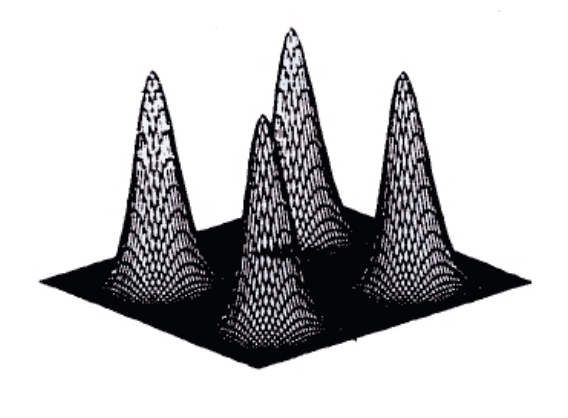
\includegraphics[width=8cm, keepaspectratio]{capitoli/immagini/imgs/puzzante.png}
    \caption{Nell'immagine possiamo osservare l'andamento pulsante della funzione campionante.}
\end{figure}

\section{Quantizzazione}
Per ottenere una completa discretizzazione di un'immagine è necessario
discretizzare, oltre al dominio, anche l'insieme immagine (insieme dei valori).
\begin{definition}
    Si definisce \textbf{quantizzazione} il procedimento di discretizzazione dei
    valori della funzione che rappresenta un'immagine, cioè il passaggio da
    valori continui a valori discreti.
\end{definition}
Per le immagini a toni di grigio si parla di \textbf{grey level quantization},
mentre per le immagini a colori si parla di \textbf{color depth}, in riferimento
al numero di bit utilizzati per ciascun canale di colore (8, 16, 24, 32 bit).
\begin{itemize}
    \item \textbf{Esempio 1:} Le immagini che siamo abituati a vedere tutti i giorni sui nostri cellulari
          sono immagini a colori a 8bit.
    \item \textbf{Esempio 2:} Nelle immagini mediche, di solito in formato
          \textbf{DICOM}, le immagini vengono rappresentate a 16bit ma gli
          ultimi 4 bit dell'immagine sono riservati ad informazioni personali
          che servono ad identificare il paziente che ha sostenuto l'esame.
\end{itemize}
\section{Immagine Digitale}
Tramite il campionamento e la quantizzazione è possibile definire un'immagine
digitale come segue:
\begin{definition}
    Una immagine digitale è una rappresentazione di matrici di elementi
    immagine, detti anche pixel (pixel = picture elements). Dove

    \begin{itemize}
        \item Il \textbf{pixel} costituisce la componente elementare della matrice,
              dove gli indici di riga e colonna indicano i valori delle due
              variabili spaziali, cioè la posizione di un punto nell'immagine.
        \item Ogni elemento della matrice contiene i valori che rappresentano
              l'intensità dei corrispondenti punti nell'immagine, anche detta
              \textbf{luminanza}.
    \end{itemize}
\end{definition}

\section{Campionamento per Immagini}
L'Immagine campionata è rappresentata tramite la seguente formula:

$$
    f_c(x,y) = f(x,y)s_c(x,y)=f(x,y)\sum_{j=-\infty}^{+\infty}
    \sum_{k=-\infty}^{+\infty} \delta (x-j \Delta x, y-k \Delta y)
$$

dove $s_c(x,y)$ è \textbf{la funzione campionante} e $\delta$ rappresenta
funzione \textbf{delta di Dirac} \TODO[]{Definire funzione di Dirac}.\\

Si può provare che c'è una relazione tra $\hat{f}_c$ e $\hat{f}$. Per questo è
importante assumere che lo spettro del segnale $f$ sia \textbf{a banda
    limitata}, cioè:

$$
    \hat{f}(\omega_x, \omega_y)=0 \text{ per } |\omega_x| > \bar{\omega}_x \text{ e } |\omega_y| > \bar{\omega}_y
$$
dove $\bar{\omega}_x$ e $\bar{\omega}_y$ definiscono la banda rettangolare dell'immagine.\\

Così lo spettro dell'immagine campionata consiste nello spettro dell'immagine
continua infinitamente ripetuta nel piano delle frequenze, in una griglia di
risoluzione ($\frac{2\pi}{\Delta x}, \frac{2 \pi}{\Delta y}$), dove:

$$
    (\frac{2\pi}{\Delta x}, \frac{2 \pi}{\Delta y}) = (w_{xc}, w_{yc})
$$

sono le \textbf{frequenze Sampling}.\\

Per ricostruire esattamente un segnale
campionato, la frequenza del campionamento non deve essere inferiore ad una
\textbf{frequenza minima (ovvero frequenza sampling)}, che corrisponde ad un
valore massimo per ciascuno degli intervalli $\Delta x$ , $\Delta y$.\\

Tale
valore minimo deve essere almeno pari al doppio della banda massima di $f$ ,
cioè:

\begin{equation}\label{eq:launo}
    \omega_{xc} \geq 2 \bar{\omega}_x \text{ e } \omega_{yc} \geq 2 \bar{\omega}_y
\end{equation}

o equivalentemente:

$$
    \frac{1}{\Delta x} \ge 2 \bar{\omega_x} \ \text{ e } \frac{1}{\Delta y} \ge 2 \bar{\omega_y}
$$
%% questa era LA UNO
Se nella (\ref{eq:launo}) vale l'uguaglianza, allora si dice che l'immagine è
\textbf{campionata alla sua frequenza di Nyquist.}\\

Se $\Delta x$ e $\Delta y$ sono più piccoli del richiesto criterio di
Nyquist, l'immagine risulta sovracampionata \textbf{(oversampling)}. Nel caso
contrario, l'immagine non può essere ricostruita esattamente: si parla di
sottocampionamento \textbf{(undersampling)} e si presenta un fenomeno di
distorsione detto \textbf{aliasing.}

\paragraph{Note:}
\begin{itemize}
    \item il valore minimo è un valore puramente teorico. Nella pratica, non
          potendo in generale determinare con precisione la banda massima del
          segnale, si utilizzano frequenze di campionamento più alte. Spesso
          si campiona con una frequenza pari a 4 volte quella misurata.
\end{itemize}

\begin{theorem}[Teorema del Campionamento per Immagini]
    Sia $f(x,y)$ un' immagine
    \begin{itemize}
        \item a banda limitata e ad energia finita, soddisfa quindi
              $$
                  \hat{f}(\omega_x,\omega_y) = 0 \text{ per } | \omega_x | >
                  \bar{\omega}_x \text{ e } | \omega_y | > \bar{\omega}_y;
              $$
        \item con $f$ uniformemente campionata in una
              griglia rettangolare con intervalli spaziali $\Delta x$, $\Delta y$,
        \item che abbia l'ordine di campionamento più grande dell'ordine di
              Nyquist, cioè
              $$
                  \omega_{xc} \geq 2 \bar{\omega}_x, \ \omega_{yc} \geq 2 \bar{\omega}_y
              $$
    \end{itemize}

    allora
    la $f$ può essere ricostruita dai suoi valori campione $f(j \Delta x, k
        \Delta y)$. Inoltre, l'immagine ricostruita è data dalla seguente formula di
    interpolazione:
\end{theorem}

$$
    f(x,y) = \sum_{j=-\infty}^{+\infty} \sum_{k=-\infty}^{+\infty} f(j \Delta
    x, k \Delta y) (\frac{\sin(xw_{xc}-j)\pi}{(xw_{xc}-j)\pi})
    (\frac{\sin(yw_{yc}-k)\pi}{(yw_{yc}-k)\pi})
$$

\section{L'aliasing}

Per ricostruire esattamente una immagine, è necessario limitare in banda
l'immagine che deve essere campionata, campionando all'ordine di campionamento
di Nyquist o più grande e interpolando appropriatamente i valori immagine.
\\\\Se c'è sovrapposizione di spettri, risultante dal sottocampionamento, vuol
dire che componenti spettrali spurie sono state introdotte nel processo di
ricostruzione. L'effetto che si ottiene è chiamato aliasing.

\begin{figure}[H]
    \centering
    \begin{tikzpicture}[x=0.75pt,y=0.75pt,yscale=-1,xscale=1]
        %uncomment if require: \path (0,300); %set diagram left start at 0, and has height of 300

        %Shape: Axis 2D [id:dp6614397845308091] 
        \draw  (204,230.75) -- (542.5,230.75)(306,82) -- (306,250.25) (535.5,225.75) -- (542.5,230.75) -- (535.5,235.75) (301,89) -- (306,82) -- (311,89)  ;
        %Straight Lines [id:da059819649685002974] 
        \draw    (424.6,225.95) -- (424.6,236.45) ;
        %Curve Lines [id:da1873728797992431] 
        \draw    (269.8,230.2) .. controls (290.2,149.8) and (320.6,150.6) .. (339.4,231) ;
        %Curve Lines [id:da5724817335486379] 
        \draw    (329.4,229.8) .. controls (349.8,149.4) and (380.2,150.2) .. (399,230.6) ;
        %Curve Lines [id:da36708092911214907] 
        \draw    (388.2,230.6) .. controls (408.6,150.2) and (439,151) .. (457.8,231.4) ;
        %Curve Lines [id:da8399376612652416] 
        \draw    (211,229.8) .. controls (231.4,149.4) and (261.8,150.2) .. (280.6,230.6) ;
        %Straight Lines [id:da03322400871511211] 
        \draw  [dash pattern={on 0.84pt off 2.51pt}]  (365,170.2) -- (364.8,230.35) ;
        %Straight Lines [id:da4711905178599287] 
        \draw  [dash pattern={on 0.84pt off 2.51pt}]  (424.6,171) -- (424.4,231.15) ;
        %Straight Lines [id:da6104769152801106] 
        \draw  [dash pattern={on 0.84pt off 2.51pt}]  (246.2,170.6) -- (246,230.75) ;
        %Straight Lines [id:da17157099933830633] 
        \draw    (364.8,225.15) -- (364.8,235.65) ;
        %Straight Lines [id:da303351675318031] 
        \draw    (246.2,224.75) -- (246.2,235.25) ;
        %Shape: Free Drawing [id:dp8099197566718934] 
        \draw  [color={rgb, 255:red, 255; green, 0; blue, 0 }  ,draw opacity=1 ][line width=0.75] [line join = round][line cap = round] (275.67,216.17) .. controls (275.67,216.17) and (275.67,216.17) .. (275.67,216.17) ;
        %Shape: Free Drawing [id:dp2110659887332691] 
        \draw  [color={rgb, 255:red, 255; green, 0; blue, 0 }  ,draw opacity=1 ][line width=0.75] [line join = round][line cap = round] (275,218.17) .. controls (275,218.28) and (275,218.39) .. (275,218.5) ;
        %Shape: Free Drawing [id:dp06278082285778552] 
        \draw  [color={rgb, 255:red, 255; green, 0; blue, 0 }  ,draw opacity=1 ][line width=0.75] [line join = round][line cap = round] (275.33,218.83) .. controls (275.44,218.94) and (275.56,219.06) .. (275.67,219.17) ;
        %Shape: Free Drawing [id:dp19051968150897824] 
        \draw  [color={rgb, 255:red, 255; green, 0; blue, 0 }  ,draw opacity=1 ][line width=0.75] [line join = round][line cap = round] (275.33,219.17) .. controls (275.56,219.83) and (275.78,220.5) .. (276,221.17) ;
        %Shape: Free Drawing [id:dp6214978798746364] 
        \draw  [color={rgb, 255:red, 255; green, 0; blue, 0 }  ,draw opacity=1 ][line width=0.75] [line join = round][line cap = round] (275.67,219.83) .. controls (276.11,220.39) and (276.56,220.94) .. (277,221.5) ;
        %Shape: Free Drawing [id:dp9117399273678792] 
        \draw  [color={rgb, 255:red, 255; green, 0; blue, 0 }  ,draw opacity=1 ][line width=0.75] [line join = round][line cap = round] (277.33,221.5) .. controls (278.33,222.17) and (278.86,223.4) .. (279.33,224.5) ;
        %Shape: Free Drawing [id:dp9439140035486251] 
        \draw  [color={rgb, 255:red, 255; green, 0; blue, 0 }  ,draw opacity=1 ][line width=0.75] [line join = round][line cap = round] (277.33,223.17) .. controls (277.22,223.17) and (277.11,223.17) .. (277,223.17) ;
        %Shape: Free Drawing [id:dp30388898253809615] 
        \draw  [color={rgb, 255:red, 255; green, 0; blue, 0 }  ,draw opacity=1 ][line width=0.75] [line join = round][line cap = round] (275,221.83) .. controls (274.89,222.72) and (274.78,223.61) .. (274.67,224.5) ;
        %Shape: Free Drawing [id:dp1381324474200707] 
        \draw  [color={rgb, 255:red, 255; green, 0; blue, 0 }  ,draw opacity=1 ][line width=0.75] [line join = round][line cap = round] (275.67,223.17) .. controls (276.22,223.72) and (276.78,224.28) .. (277.33,224.83) ;
        %Shape: Free Drawing [id:dp8005021491573696] 
        \draw  [color={rgb, 255:red, 255; green, 0; blue, 0 }  ,draw opacity=1 ][line width=0.75] [line join = round][line cap = round] (277.67,225.5) .. controls (277.67,226.61) and (277.67,227.72) .. (277.67,228.83) ;
        %Shape: Free Drawing [id:dp2674763078018507] 
        \draw  [color={rgb, 255:red, 255; green, 0; blue, 0 }  ,draw opacity=1 ][line width=0.75] [line join = round][line cap = round] (276.67,228.17) .. controls (276.33,227.83) and (276,227.5) .. (275.67,227.17) ;
        %Shape: Free Drawing [id:dp7006529540548063] 
        \draw  [color={rgb, 255:red, 255; green, 0; blue, 0 }  ,draw opacity=1 ][line width=0.75] [line join = round][line cap = round] (274.33,226.17) .. controls (274.33,225.94) and (274.33,225.72) .. (274.33,225.5) ;
        %Shape: Free Drawing [id:dp12114685025543515] 
        \draw  [color={rgb, 255:red, 255; green, 0; blue, 0 }  ,draw opacity=1 ][line width=0.75] [line join = round][line cap = round] (274.33,222.83) .. controls (274.33,222.94) and (274.33,223.06) .. (274.33,223.17) ;
        %Shape: Free Drawing [id:dp11181613935726564] 
        \draw  [color={rgb, 255:red, 255; green, 0; blue, 0 }  ,draw opacity=1 ][line width=0.75] [line join = round][line cap = round] (272.33,227.5) .. controls (272.44,227.61) and (272.56,227.72) .. (272.67,227.83) ;
        %Shape: Free Drawing [id:dp21874941104891454] 
        \draw  [color={rgb, 255:red, 255; green, 0; blue, 0 }  ,draw opacity=1 ][line width=0.75] [line join = round][line cap = round] (276.33,226.5) .. controls (276.33,226.5) and (276.33,226.5) .. (276.33,226.5) ;
        %Shape: Free Drawing [id:dp1551213334904571] 
        \draw  [color={rgb, 255:red, 255; green, 0; blue, 0 }  ,draw opacity=1 ][line width=0.75] [line join = round][line cap = round] (336,225.5) .. controls (336,225.5) and (336,225.5) .. (336,225.5) ;
        %Shape: Free Drawing [id:dp5552556558692121] 
        \draw  [color={rgb, 255:red, 255; green, 0; blue, 0 }  ,draw opacity=1 ][line width=0.75] [line join = round][line cap = round] (335.67,223.83) .. controls (335.44,223.61) and (335.22,223.39) .. (335,223.17) ;
        %Shape: Free Drawing [id:dp2680712522684394] 
        \draw  [color={rgb, 255:red, 255; green, 0; blue, 0 }  ,draw opacity=1 ][line width=0.75] [line join = round][line cap = round] (335,222.5) .. controls (334.78,222.06) and (334.56,221.61) .. (334.33,221.17) ;
        %Shape: Free Drawing [id:dp7973466921888765] 
        \draw  [color={rgb, 255:red, 255; green, 0; blue, 0 }  ,draw opacity=1 ][line width=0.75] [line join = round][line cap = round] (334,223.17) .. controls (333.67,223.72) and (333.33,224.28) .. (333,224.83) ;
        %Shape: Free Drawing [id:dp4217427243501193] 
        \draw  [color={rgb, 255:red, 255; green, 0; blue, 0 }  ,draw opacity=1 ][line width=0.75] [line join = round][line cap = round] (331.67,227.83) .. controls (331.67,227.83) and (331.67,227.83) .. (331.67,227.83) ;
        %Shape: Free Drawing [id:dp7263061231203432] 
        \draw  [color={rgb, 255:red, 255; green, 0; blue, 0 }  ,draw opacity=1 ][line width=0.75] [line join = round][line cap = round] (334,227.83) .. controls (334,227.83) and (334,227.83) .. (334,227.83) ;
        %Shape: Free Drawing [id:dp5942130285250151] 
        \draw  [color={rgb, 255:red, 255; green, 0; blue, 0 }  ,draw opacity=1 ][line width=0.75] [line join = round][line cap = round] (334.33,227.83) .. controls (334.33,227.83) and (334.33,227.83) .. (334.33,227.83) ;
        %Shape: Free Drawing [id:dp15743052029399962] 
        \draw  [color={rgb, 255:red, 255; green, 0; blue, 0 }  ,draw opacity=1 ][line width=0.75] [line join = round][line cap = round] (335.33,227.83) .. controls (335.78,228.06) and (336.22,228.28) .. (336.67,228.5) ;
        %Shape: Free Drawing [id:dp22495918083215116] 
        \draw  [color={rgb, 255:red, 255; green, 0; blue, 0 }  ,draw opacity=1 ][line width=0.75] [line join = round][line cap = round] (334.67,226.5) .. controls (334.67,226.5) and (334.67,226.5) .. (334.67,226.5) ;
        %Shape: Free Drawing [id:dp2784909236606581] 
        \draw  [color={rgb, 255:red, 255; green, 0; blue, 0 }  ,draw opacity=1 ][line width=0.75] [line join = round][line cap = round] (336.33,220.83) .. controls (336.33,220.94) and (336.33,221.06) .. (336.33,221.17) ;
        %Shape: Free Drawing [id:dp8706240640891032] 
        \draw  [color={rgb, 255:red, 255; green, 0; blue, 0 }  ,draw opacity=1 ][line width=0.75] [line join = round][line cap = round] (335.33,220.5) .. controls (335.22,220.5) and (335.11,220.5) .. (335,220.5) ;
        %Shape: Free Drawing [id:dp9329750308424989] 
        \draw  [color={rgb, 255:red, 255; green, 0; blue, 0 }  ,draw opacity=1 ][line width=0.75] [line join = round][line cap = round] (392.67,227.83) .. controls (393,228.06) and (393.33,228.28) .. (393.67,228.5) ;
        %Shape: Free Drawing [id:dp3882317480429962] 
        \draw  [color={rgb, 255:red, 255; green, 0; blue, 0 }  ,draw opacity=1 ][line width=0.75] [line join = round][line cap = round] (395,228.17) .. controls (395.63,228.8) and (395.3,228.46) .. (394.67,227.83) ;
        %Shape: Free Drawing [id:dp4131517984324593] 
        \draw  [color={rgb, 255:red, 255; green, 0; blue, 0 }  ,draw opacity=1 ][line width=0.75] [line join = round][line cap = round] (394.33,224.5) .. controls (395,224.83) and (395.67,225.17) .. (396.33,225.5) ;
        %Shape: Free Drawing [id:dp37363169850637656] 
        \draw  [color={rgb, 255:red, 255; green, 0; blue, 0 }  ,draw opacity=1 ][line width=0.75] [line join = round][line cap = round] (394,227.83) .. controls (393.78,227.5) and (393.56,227.17) .. (393.33,226.83) ;
        %Shape: Free Drawing [id:dp11367818680791109] 
        \draw  [color={rgb, 255:red, 255; green, 0; blue, 0 }  ,draw opacity=1 ][line width=0.75] [line join = round][line cap = round] (393,219.83) .. controls (392.89,219.5) and (392.78,219.17) .. (392.67,218.83) ;
        %Shape: Free Drawing [id:dp0009232964570280444] 
        \draw  [color={rgb, 255:red, 255; green, 0; blue, 0 }  ,draw opacity=1 ][line width=0.75] [line join = round][line cap = round] (394.33,220.5) .. controls (394.67,221.17) and (395,221.83) .. (395.33,222.5) ;
        %Shape: Free Drawing [id:dp980765288470274] 
        \draw  [color={rgb, 255:red, 255; green, 0; blue, 0 }  ,draw opacity=1 ][line width=0.75] [line join = round][line cap = round] (392.33,219.83) .. controls (392.33,221.28) and (392.33,222.72) .. (392.33,224.17) ;
        %Shape: Free Drawing [id:dp18690833347628333] 
        \draw  [color={rgb, 255:red, 255; green, 0; blue, 0 }  ,draw opacity=1 ][line width=0.75] [line join = round][line cap = round] (394,224.17) .. controls (394.11,224.17) and (394.22,224.17) .. (394.33,224.17) ;
        %Shape: Free Drawing [id:dp5757936876425502] 
        \draw  [color={rgb, 255:red, 255; green, 0; blue, 0 }  ,draw opacity=1 ][line width=0.75] [line join = round][line cap = round] (392.67,225.17) .. controls (392.67,225.17) and (392.67,225.17) .. (392.67,225.17) ;
        %Shape: Free Drawing [id:dp3612108432226979] 
        \draw  [color={rgb, 255:red, 255; green, 0; blue, 0 }  ,draw opacity=1 ][line width=0.75] [line join = round][line cap = round] (392.67,226.5) .. controls (392.89,226.61) and (393.11,226.72) .. (393.33,226.83) ;
        %Shape: Free Drawing [id:dp7648800367951516] 
        \draw  [color={rgb, 255:red, 255; green, 0; blue, 0 }  ,draw opacity=1 ][line width=0.75] [line join = round][line cap = round] (394.67,218.83) .. controls (394.67,218.83) and (394.67,218.83) .. (394.67,218.83) ;
        %Shape: Free Drawing [id:dp1400767539639749] 
        \draw  [color={rgb, 255:red, 255; green, 0; blue, 0 }  ,draw opacity=1 ][line width=0.75] [line join = round][line cap = round] (397.67,226.17) .. controls (397.67,226.5) and (397.67,226.83) .. (397.67,227.17) ;
        %Straight Lines [id:da9749345597918087] 
        \draw [color={rgb, 255:red, 0; green, 0; blue, 0 }  ,draw opacity=1 ]   (394.33,138.5) -- (394.33,197.83) ;
        \draw [shift={(394.33,199.83)}, rotate = 270] [color={rgb, 255:red, 0; green, 0; blue, 0 }  ,draw opacity=1 ][line width=0.75]    (10.93,-3.29) .. controls (6.95,-1.4) and (3.31,-0.3) .. (0,0) .. controls (3.31,0.3) and (6.95,1.4) .. (10.93,3.29)   ;
        %Straight Lines [id:da9406931472834237] 
        \draw    (394.33,138.5) -- (450.67,138.83) ;
        %Straight Lines [id:da7746905723182127] 
        \draw  [dash pattern={on 0.84pt off 2.51pt}]  (339.07,151) -- (339.4,231) ;
        %Straight Lines [id:da7675893385629211] 
        \draw    (305.67,150.17) -- (337.07,150.95) ;
        \draw [shift={(339.07,151)}, rotate = 181.43] [color={rgb, 255:red, 0; green, 0; blue, 0 }  ][line width=0.75]    (10.93,-3.29) .. controls (6.95,-1.4) and (3.31,-0.3) .. (0,0) .. controls (3.31,0.3) and (6.95,1.4) .. (10.93,3.29)   ;

        % Text Node
        \draw (308.8,231.8) node [anchor=north west][inner sep=0.75pt]   [align=left] {0};
        % Text Node
        \draw (356,239.4) node [anchor=north west][inner sep=0.75pt]    {$f_{S}$};
        % Text Node
        \draw (411.2,240.6) node [anchor=north west][inner sep=0.75pt]    {$2f_{S}$};
        % Text Node
        \draw (230.4,240.2) node [anchor=north west][inner sep=0.75pt]    {$-f_{S}$};
        % Text Node
        \draw (398.67,119.67) node [anchor=north west][inner sep=0.75pt]   [align=left] {Aliasing};
        % Text Node
        \draw (309.67,128.73) node [anchor=north west][inner sep=0.75pt]    {$f_{m}$};
    \end{tikzpicture}
    \caption{Visualizzazione della sovrapposizione degli spettri che genera aliasing}
\end{figure}

Quindi l'aliasing è la presenza di componenti spettrali (frequenze) indesiderate
nella ricostruzione dell'immagine, componenti che non erano presenti quando
l'immagine originale era stata campionata.

\begin{figure}[H]
    \centering
    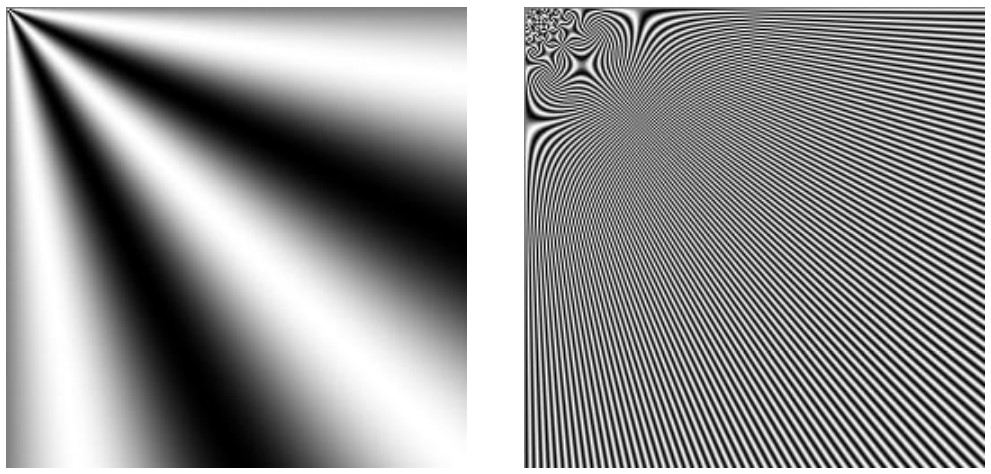
\includegraphics[width=10cm, keepaspectratio]{capitoli/immagini/imgs/aliasing_componenti_spettrali.jpg}
    \caption{Esempio di frequenze indesiderate prodotte dall'aliasing.}
\end{figure}

L'aliasing deriva dal sottocampionamento e causa perdita di risoluzione
dell'immagine campionata (effetto scacchiera).

\begin{figure}[H]
    \centering
    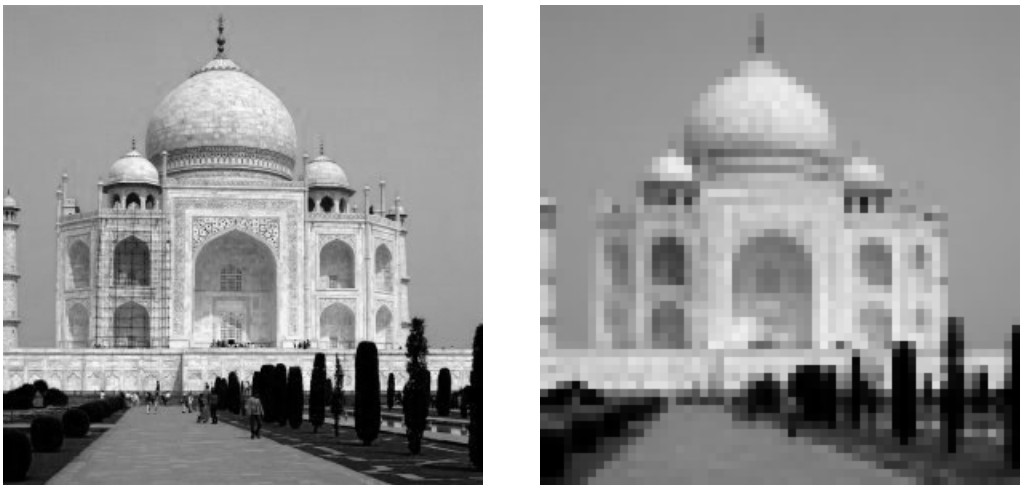
\includegraphics[width=10cm, keepaspectratio]{capitoli/immagini/imgs/aliasing_tajmahal.jpg}
    \caption{Esempio di effetto a scacchiera generato dall'aliasing}.
\end{figure}

\begin{itemize}
    \item Per prevenire aliasing di queste componenti, è possibile filtrarle via
          (eliminarle) prima di campionare il segnale. Eliminare certe frequenze
          e lasciare passare le basse frequenze, è una operazione nota come
          \textbf{filtraggio passa-basso}.
    \item Ogni attenuazione relativa a questo processo di filtraggio rappresenta
          una perdita di risoluzione dell'immagine campionata.
    \item Come risultato, mentre da un lato c'è una perdita della risoluzione
          dell'immagine campionata, dall'altro c'è una attenuazione
          dell'aliasing error.
    \item \textbf{Effetto Moirè:} ovvero la distorsione visiva che si manifesta
          quando due griglie si sovrappongono
          \begin{figure}[H]
              \centering
              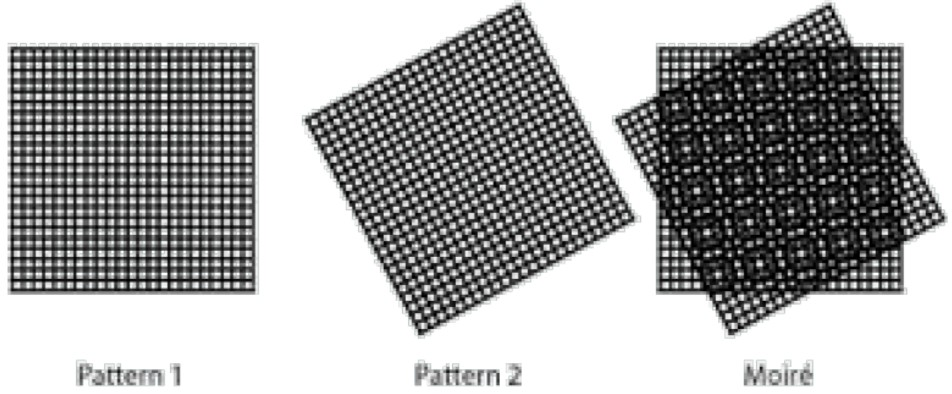
\includegraphics[width=8cm, keepaspectratio]{capitoli/immagini/imgs/effetto_moire.jpg}
          \end{figure}
\end{itemize}

\section{La risoluzione}
Il campionamento e la quantizzazione determinano la \textbf{risoluzione}
dell'immagine. \\

La \textbf{risoluzione} di un segnale è un indice del grado
di qualità dell'immagine: misura il grado di oggetti distinguibili
nell'immagine. Esistono differenti definizione di risoluzione:

\begin{definition}
    La \textbf{Risoluzione Spaziale} indica la densità dei campioni, ovvero è data dal numero di campioni
    per unità di area.
\end{definition}

Spesso è espressa come numero di pixel
nell'unità di lunghezza e viene misurata in pixel per pollice (ppi).
\\Un'immagine ad alta risoluzione contiene più pixel di una delle
stesse dimensioni con una risoluzione inferiore, quindi è in grado di
riprodurre un maggior numero di dettagli. Un'elevata risoluzione
comporta tuttavia un aumento considerevole delle dimensioni (quantità
di dati) dell'immagine.

\paragraph{Esempio:}

Un'immagine di $1cm \times 1cm$ con una risoluzione di 72 ppi
contiene 5184 pixel ($72 \times 72$). La stessa immagine di $1 cm \times
    1 cm$ a 300 ppi conterrebbe 90.000 pixel.

\begin{definition}
    La \textbf{Risoluzione spettrale} indica la banda passante del sensore.

\end{definition}


\begin{definition}
    \textbf{Risoluzione radiometrica} indica il numero di livelli di quantizzazione.

\end{definition}


\begin{definition}
    \textbf{Risoluzione temporale} indica la frequenza di acquisizione dei frames di un'immagine in
    movimento.
\end{definition}

\section{Alterazioni della risoluzione}

Alterando i vari tipi di risoluzione, l'immagine presenterà di volta in volta un
diverso tipo di distorsione.

\begin{trivlist}
    \item \textbf{Risoluzione spaziale:} diminuendo la risoluzione spaziale
    (nell'esempio di un quarto) si ottiene il tipico effetto ”quadrettato”,
    detto anche a scacchiera, dovuto all'aliasing.
    \begin{figure}[H]
        \centering
        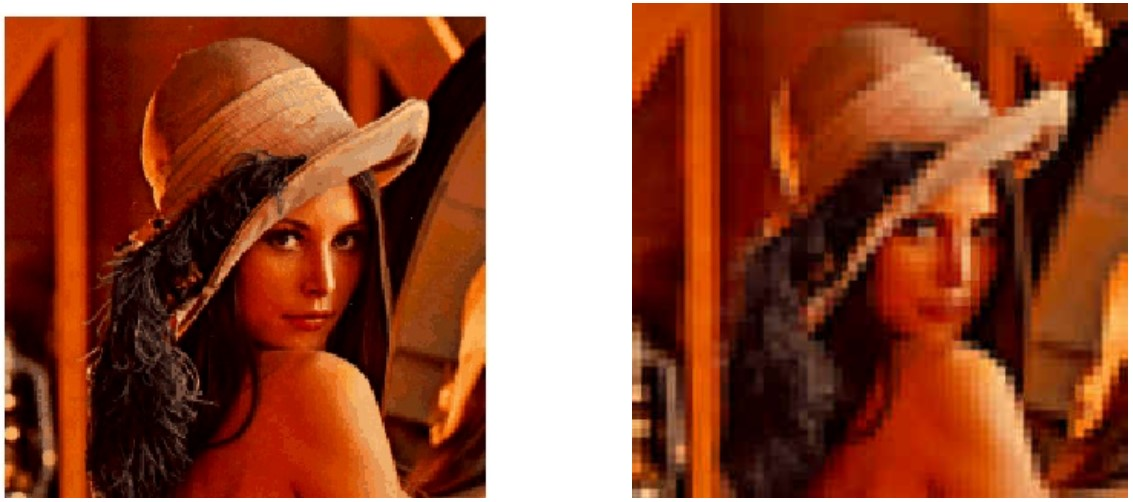
\includegraphics[width=10cm, keepaspectratio]{capitoli/immagini/imgs/esempio_risoluzione_spaziale.jpg}
    \end{figure}

    \item \textbf{Risoluzione spettrale:} Diminuendo la banda passante del
    sensore di acquisizione dell'immagine si ottiene un'immagine più ”sfocata”,
    in quanto i dettagli ad alta frequenza spaziale vanno persi.
    \begin{figure}[H]
        \centering
        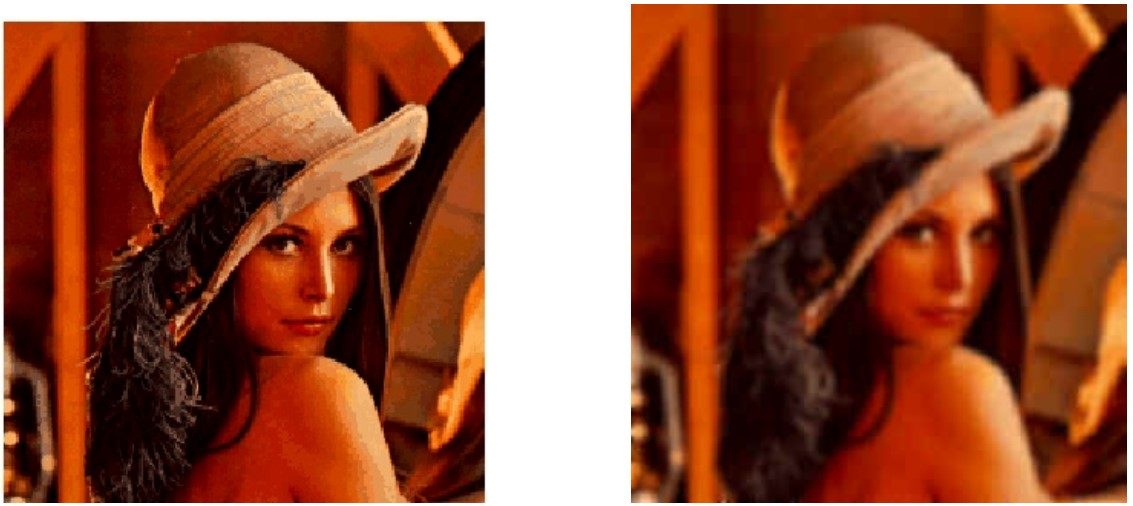
\includegraphics[width=10cm, keepaspectratio]{capitoli/immagini/imgs/esempio_risoluzione_spettrale.jpg}
    \end{figure}

    \item \textbf{Risoluzione radiometrica:} Diminuendo la profondità di colore,
    si distinguono in maniera più marcata i passaggi da un colore ad un altro;
    essi risultano pertanto sempre più accentuati e meno graduali, fino a
    produrre dei "falsi contorni" (variazioni di ombreggiatura).
    \begin{figure}[H]
        \centering
        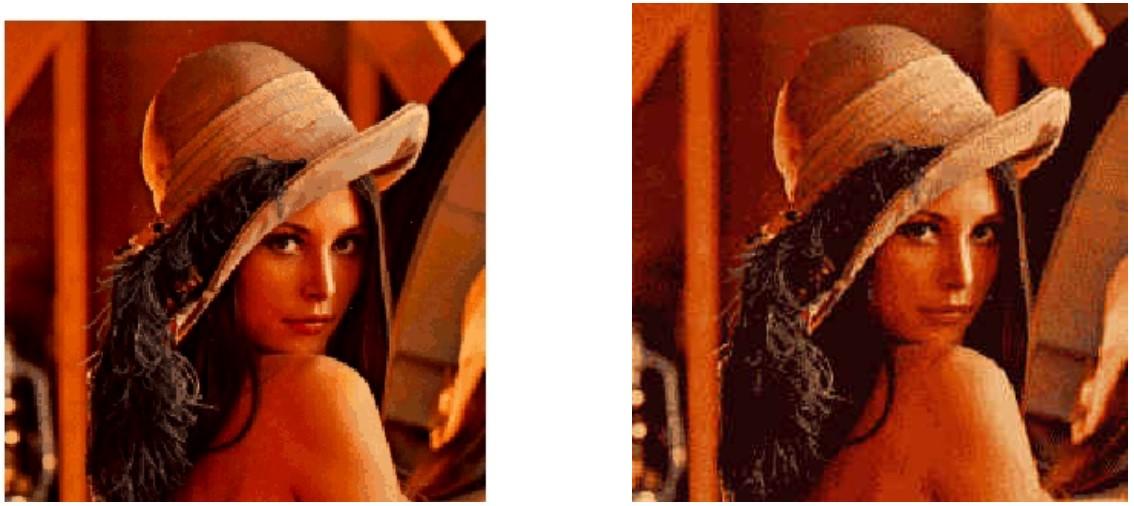
\includegraphics[width=10cm, keepaspectratio]{capitoli/immagini/imgs/esempio_risoluzione_radiometrica.jpg}
    \end{figure}
\end{trivlist}

\section{Immagini in bianco e nero e immagini a colori}

\subsection{Immagini in bianco e nero}

Un'\textbf{immagine in bianco e nero (b/w)} è caratterizzata da una
rappresentazione binaria, ovvero la funzione che la rappresenta in
ogni punto ($x$ , $y$) può assumere solo due valori: 0 e 1. In genere,
ad 1 si associa il bianco, mentre a 0 il nero.

\begin{figure}[H]
    \centering
    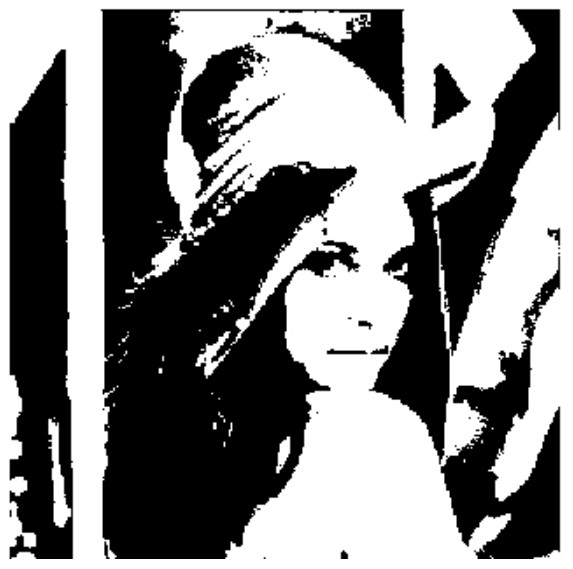
\includegraphics[width=4cm, keepaspectratio]{capitoli/immagini/imgs/immagine_binaria_bianco_nero.jpg}
    \caption{Esempio di un'immagine in bianco e nero (binaria).}
\end{figure}

\subsection{Immagini a toni di grigio}

Un'immagine a toni di grigio è rappresentata da una matrice le cui
entrate sono i valori che la funzione $f$ assume in ogni punto.

\begin{figure}[H]
    \centering
    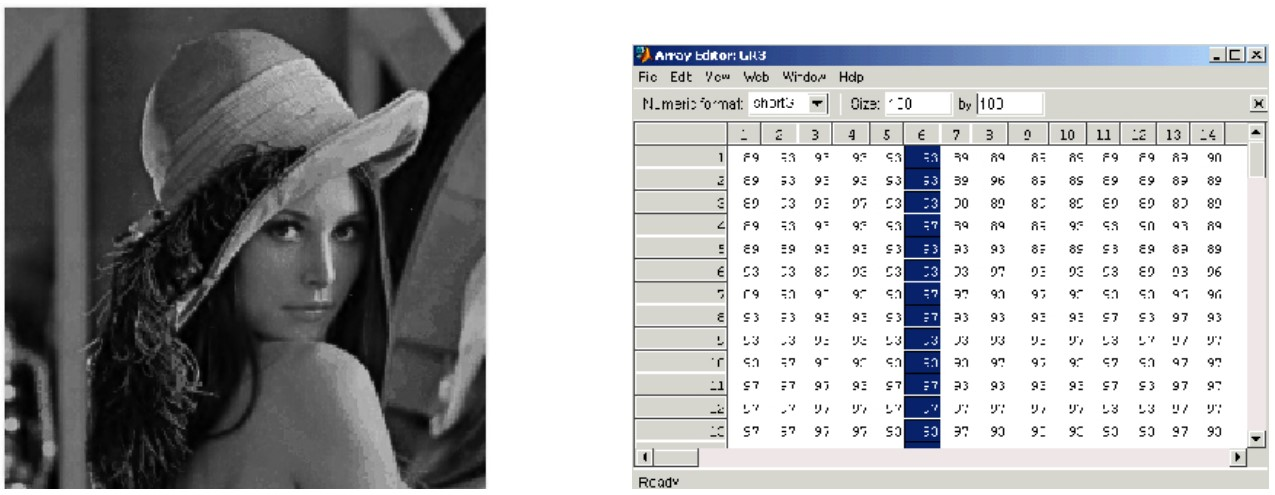
\includegraphics[width=12cm, keepaspectratio]{capitoli/immagini/imgs/rappresentazione_immagine_toni_grigio.jpg}
\end{figure}

In genere, si assume che i \textbf{livelli di grigio} siano discreti ed
equispaziati in un intervallo di valori normalmente \textbf{tra 0 e 255}:
esistono allora un massimo di 256 livelli di grigio.
\\
La funzione $f (x , y)$ può essere rappresentata come una superficie
nello spazio.

\begin{figure}[H]
    \centering
    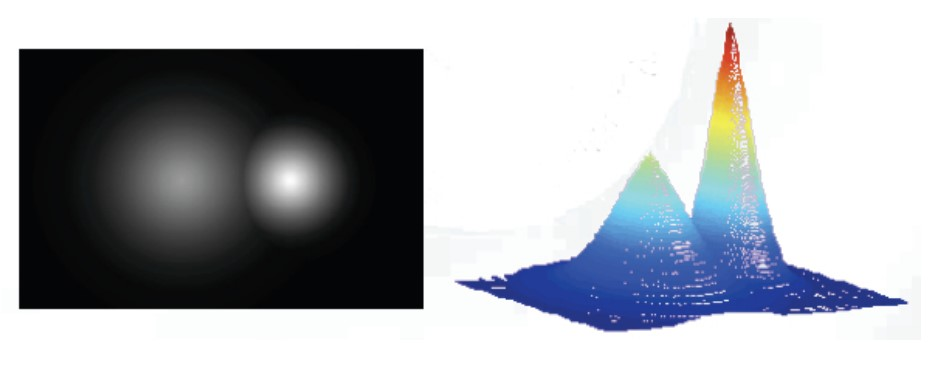
\includegraphics[width=10cm, keepaspectratio]{capitoli/immagini/imgs/funzione_toni_grigio.jpg}
\end{figure}

\subsection{Immagini a colori}

Per rappresentare un'\textbf{immagine a colori} è necessario ricorrere ad
una funzione vettoriale. Un colore infatti può essere sempre
decomposto come \textbf{somma dei tre colori fondamentali (rosso, verde,
    blu)}, ciascuno con un'opportuna intensità.
Un'immagine a colori, dunque, può essere rappresentata da una
funzione $f: \mathbb{R}^2 \rightarrow \mathbb{R}^3$ del tipo

$$
    f(x, y) = [R(x, y), G(x, y), B(x, y)]
$$

Questo tipo di rappresentazione viene detta \textbf{RGB (Red,Green,Blue)}.
\subsubsection{Lo spazio RGB}

Lo spazio RGB è uno spazio cartesiano, con tre assi ortogonali.
Il colore di ciascun pixel viene rappresentato da un vettore
$[R(x , y), G(x , y), B(x , y)]$ nello spazio RGB; ogni componente
indica la quantità di rosso, verde e blu, rispettivamente, necessari
ad ottenere quel colore.
In base alla rappresentazione RGB, un'immagine a colori viene
rappresentata da una terna di matrici, ognuna delle quali contiene i
valori relativi ad un canale di colore.\\
Ogni canale, preso a sè, non è altro che un'immagine a toni di
grigio.

\begin{figure}[H]
    \centering
    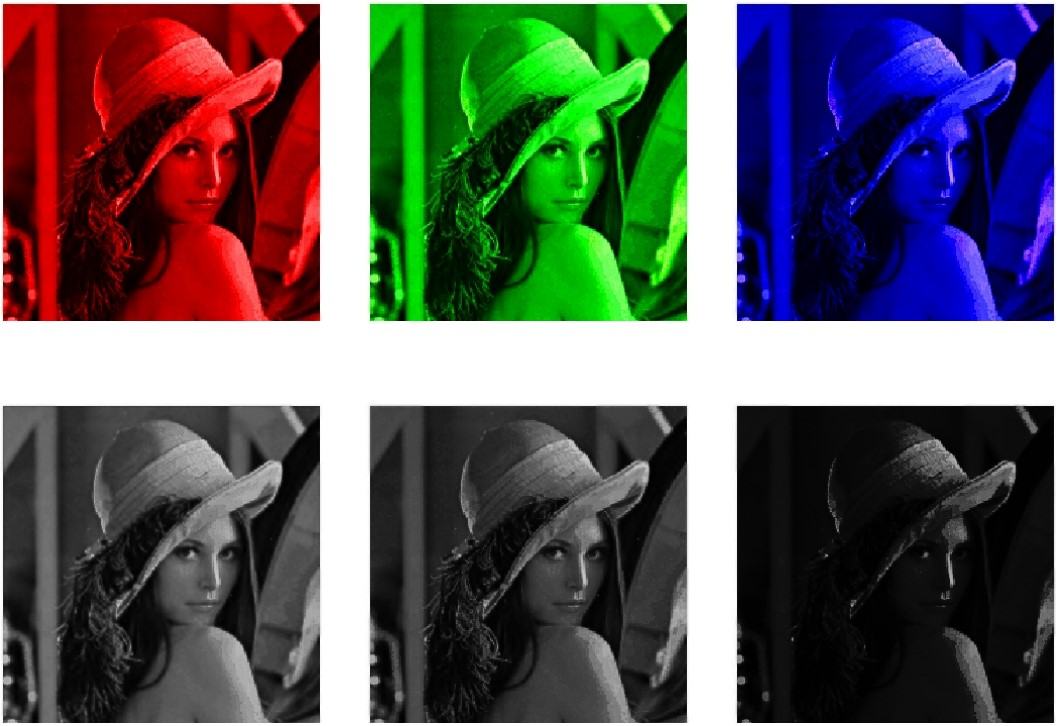
\includegraphics[width=12cm, keepaspectratio]{capitoli/immagini/imgs/canali_RGB_e_grigio.jpg}
\end{figure}

\subsubsection{Lo spazio HSV}

Oltre alla RGB esistono anche altri tipi di rappresentazioni (che
possono essere in genere derivate da essa).
Una di queste è la rappresentazione \textbf{HSV}. Lo spazio HSV ha un
sistema di coordinate cilindrico con due assi ortogonali ed un
angolo di rotazione intorno ad uno dei due assi.
L'altezza del cono rappresenta la \textbf{luminosità (Value)}, con valori da
0 (nero) a 1 (bianco). La \textbf{saturazione (Saturation)} indica l'intensità
e la purezza del colore, con valori da 0 (sull'asse del cono) a 1
(sulla superficie del cono). La terza coordinata rappresenta la
\textbf{tonalità di colore (Hue)} e viene misurata da un angolo intorno
all'asse verticale (rosso a 0 gradi, verde a 120 e blu a 240).

\begin{figure}[H]
    \centering
    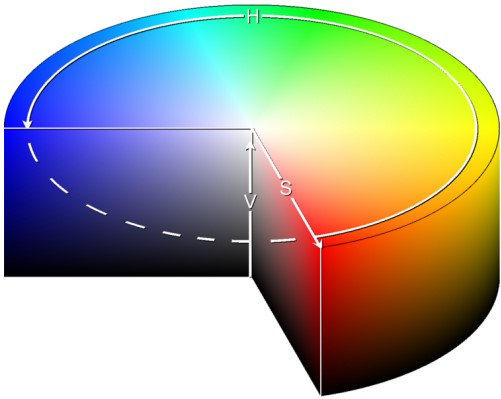
\includegraphics[width=5cm, keepaspectratio]{capitoli/immagini/imgs/cilindro_hsv.jpg}
\end{figure}


\section{Relazioni di base fra pixel}

\subsection{Intorni}

Un pixel $p$ di coordinate $(x,y)$ ha quattro \textbf{neighbors} (vicini) orizzontali e verticali:

\begin{center}
    $(x+1, y), (x-1, y), (x, y-1), (x, y+1)$
\end{center}

Questi punti formano il \textbf{4-intorno (4-neighboor)} di $(x,y)$ che indicheremo con $N_4(p)$
\\I quattro \textbf{neighbors (vicini) diagonali} di $p$ $(N_D(p))$ hanno invece coordinate

\begin{center}
    $(x+1, y+1), (x+1,y-1), (x-1, y+1), (x-1, y-1)$
\end{center}

I vicini diagonali, insieme a quelli orizzontali e verticali, formano l'\textbf{8-intorno (8-neighbor)} di $(x,y)$  che indicheremo con $N_8(p)$

\subsection{Connettività e adiacenza}

Due pixel sono connessi se sono vicini e presentano livelli di intensità con una certa relazione (ad esempio hanno lo stesso livello di grigio).
Fissato un insieme V di valori di intensità, due pixel $p$ e $q$ si dicono

\begin{itemize}
    \item \textbf{4-adiacenti} se i valori di entrambi appartengono a $V$ e $q \in N_4(p)$
    \item \textbf{8-adiacenti} se i valori di entrambi appartengono a $V$ e $q \in N_8(p)$
    \item \textbf{m-adiacenti} (adiacenza mista) se i valori di entrambi appartengono a $V$ e $q \in N_4(p)$ oppure $q \in N_D(p)$ e l'insieme $N_4(p) \cap N_4(q)$ non contiene pixel a valori in V.
\end{itemize}

\subsection{Cammini}

Un \textbf{cammino (path) digitale} dal pixel $p = (x,y)$ al pixel $q = (x',
    y')$ è una sequenza di pixel

\begin{center}
    $(x0, y0), (x1, y1), ... ,(x_n, y_n)$
\end{center}

dove $(x_0, y_0) = (x,y)$, $(x_n, y_n) = (x', y')$ e i pixel $(x_i, y_i)$,
$(x_{i+1}, y_{i+1})$ sono adiacenti per ogni $i=0, ... , n-1$, dove $n$ è la
\textbf{lunghezza del cammino}. $Se (x_0, y_0) = (x_n, y_n)$ si parla di
\textbf{cammino chiuso}. Si puo' definire in particolare un $4-$, $8-$, o
$m-$ cammino restringendo l'adiacenza alla corrispondente tipologia.

\subsection{Cammini e regioni}

Fissato un sottoinsieme $S$ di pixel di un'immagine digitale, due pixel p e q si
dicono \textbf{connessi} se esiste un cammino tra $p$ e $q$ che consiste di
pixel tutti contenuti in $S$. \\Se tutti i pixel di $S$ sono connessi, $S$ si
dice un insieme connesso: in tal caso diciamo che $S$ è una regione
dell'immagine. Il \textbf{bordo (boundary, border, contour)} di una regione $R$
è l'insieme dei pixel di $R$ che hanno uno o più vicini che non appartengono ad
R. Nel caso in cui $R$ sia l'intera immagine, il bordo si definisce come la
prima e l'ultima riga e la prima e l'ultima colonna. \\Se l'immagine contiene
$k$ regioni distinte $R_1,..., R_k$, nessuna delle quali tocca i bordi
dell'immagine, allora l'unione $R = \cup_{i=1}^n R_i$ si dice \textbf{primo
    piano (foreground)}, mentre il complementare $R^c$ viene detto
\textbf{sfondo(background)}.

\subsection{Distanza tra pixel}

Una distanza (o metrica) tra pixel è una funzione $D(p, q)$ tale che per ogni
$p, q, z$

\begin{itemize}
    \item $D(p, q) \ge 0$
    \item $D(p, q) = 0$ se e solo se $p = q$
    \item $D(p, q) = D(q, p)$
    \item $D(p, z) \le D(p, q) + D(q, z)$
\end{itemize}

\textbf{Esempi}

\begin{itemize}
    \item Distanza euclidea: $D_e(p, q) = \{(x_1 - x_2)^2 + (y_1 - y_2)^2\}^{\frac{1}{2}}$, se $p = (x_1, y_1), q=(x_2, y_2)$
    \item Distanza $D_4$, o city-block: $D_4(p, q) = |x_1 - x_2| + |y_1 - y_2|$.
    \item Distanza $D_8$, o a scacchiera: $D_s(p,q) = max\{|x_1 - x_2|, |y_1 - y_2|\}$
\end{itemize}

\chapter{Elaborazione con Filtri}

L'elaborazione delle immagini è una disciplina che prevede l'utilizzo
di algoritmi i quali operano sui pixel che compongono l'immagine
e, applicando trasformazioni numeriche, restituiscono un'immagine
modificata.\\
Le tecniche di elaborazione delle immagini hanno vari scopi, fra cui:

\begin{itemize}
    \item il miglioramento della qualità dell'immagine (\textbf{image enhancement})
    \item il ripristino della qualità dell'immagine (\textbf{image restoration})
    \item l'estrazione di informazioni sul contenuto dell'immagine (\textbf{image analysis})
\end{itemize}

\paragraph{Note:}

\begin{itemize}
    \item L'\textbf{image analysis} è una parte fondamentale della computer vision e
          precede l'\textbf{image recognition}.\\
          Essa può richiedere elaborazioni differenti a seconda del tipo di
          informazione che si vuole estrarre: tra queste, le elaborazioni nel
          dominio spaziale, nel dominio delle frequenze, con riduzione dei
          dati tra ingresso e uscita (compressione), etc.
\end{itemize}

\paragraph{Esempio:}

Un'elaborazione nel dominio spaziale, può essere
espressa come

$$
    g(x , y) = T(f (x , y))
$$

\begin{itemize}
    \item $f$ è l'immagine di ingresso
    \item $g$ è l'immagine di uscita
    \item $T$ è un operatore su f, definito in un intorno di $(x , y)$.
\end{itemize}

La natura dell'intorno definisce il tipo di elaborazione e si distingue,
in particolare, fra: \textbf{elaborazioni puntuali}, \textbf{locali} e \textbf{globali}.

\begin{definition}
    Le elaborazioni \textbf{puntuali} trasformano il valore di un pixel sulla
    base del valore del pixel stesso.
\end{definition}

\begin{definition}
    Le elaborazioni \textbf{locali} lavorano sulla base dei valori assunti dai pixel in
    un intorno di quello preso in esame.
\end{definition}

\begin{definition}
    Le elaborazioni \textbf{globali} trasformano il valore di un pixel sulla
    base dei valori assunti da tutti i pixel dell'immagine.
\end{definition}

\section{Elaborazioni Locali}

\subsection{Zoom}

Si crea una nuova griglia, ovvero delle nuove "locazioni" per i pixel,
sovrapponendola a quella originale; si assegnano poi i livelli di grigio a
queste nuove locazioni.

\begin{itemize}
    \item \textbf{Nearest Neighbor:} assegna ad ogni nuova locazione l'intensità
          del pixel più vicino dell'immagine originale

    \item \textbf{Interpolazione bilineare:} prevede l'utilizzo dei quattro
          pixel più vicini per stimare l'intensità da assegnare ad ogni nuova
          locazione

          \begin{figure}[H]
              \centering
              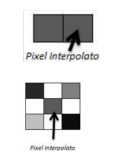
\includegraphics[width=3cm, keepaspectratio]{capitoli/immagini/imgs/esempio-interpolazione.png}
          \end{figure}

          $$
              f(x,y)=ax+by+cxy+d
          $$

          dove i coefficienti $a, b, c, d$ sono determinati dal seguente sistema
          lineare di 4 equazioni in 4 incognite:

          $$
              \left\{\begin{array}{l}
                  f\left(x_0, y_0\right)=a x_0+b y_0+c x_0 y_0+d \\
                  f\left(x_0, y_1\right)=a x_0+b y_1+c x_0 y_1+d \\
                  f\left(x_1, y_0\right)=a x_1+b y_0+c x_1 y_0+d \\
                  f\left(x_1, y_1\right)=a x_1+b y_1+c x_1 y_1+d
              \end{array}\right.
          $$

          \begin{figure}[H]
              \centering
              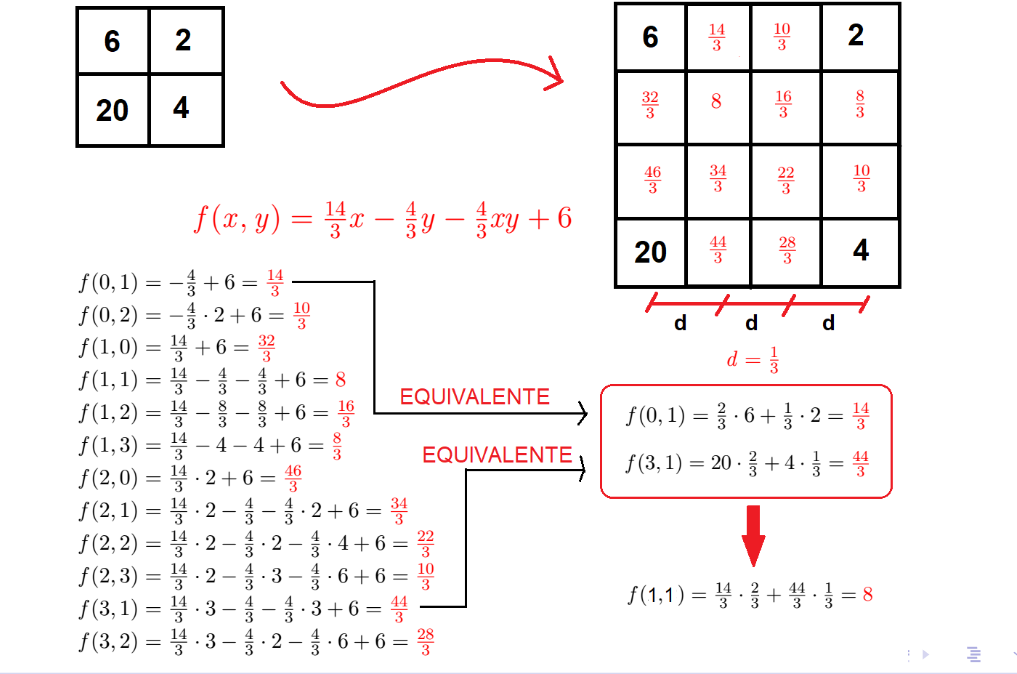
\includegraphics[width=10cm, keepaspectratio]{capitoli/immagini/imgs/calcolo_bilineare.png}
              \caption{Esempio di svolgimento di uno zoom con interpolazione bilineare.}
          \end{figure}

    \item \textbf{Interpolazione bicubica:} prevede l'utilizzo dei sedici pixel
          più vicini per stimare l'intensità da assegnare ad ogni nuova
          locazione.

          \begin{figure}[H]
              \centering
              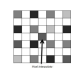
\includegraphics[width=3cm, keepaspectratio]{capitoli/immagini/imgs/interpolazione-bicubica.png}
          \end{figure}

\end{itemize}


\subsection{Shrink}

Lo stesso procedimento dello zoom, con una griglia immaginaria di dimensioni inferiori all'originale.
Per fattori interi si procede come nel caso dello zoom, ma per cancellazione di righe e colonne.

\begin{figure}[H]
    \centering
    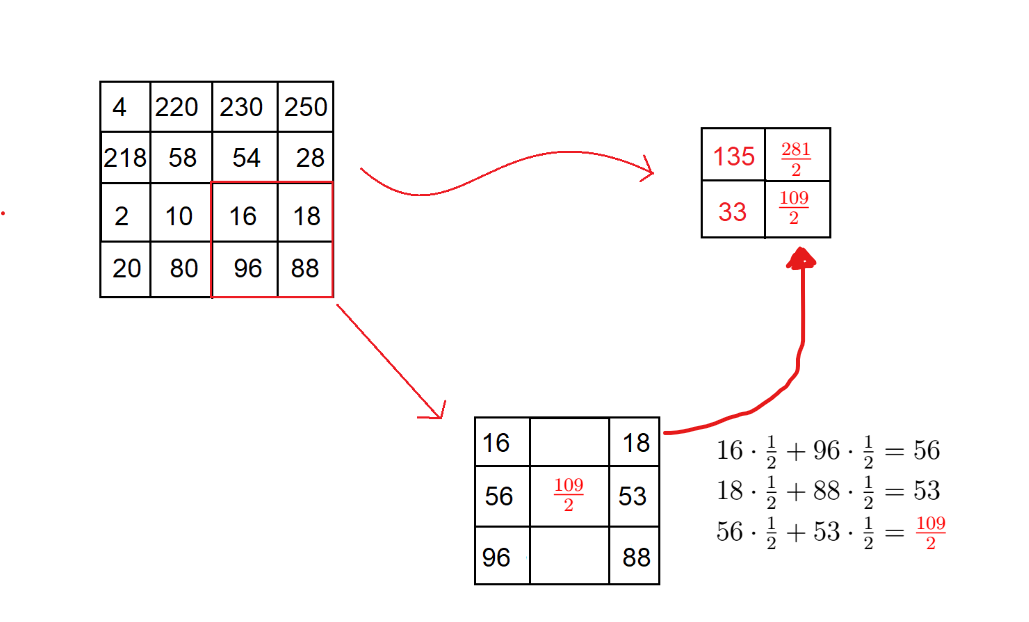
\includegraphics[width=10cm, keepaspectratio]{capitoli/immagini/imgs/calcolo_shrink.png}
    \caption{Esempio di svolgimento di uno shrink.}
\end{figure}

\section{Elaborazioni Puntuali}

\begin{definition}
    Un'elaborazione puntuale si dice \textbf{omogenea} se il risultato
    dipende solo dal valore (in scala di grigi) del pixel a cui è applicata.\\
    Se invece il risultato dipende anche dalla posizione del pixel,
    l'elaborazione puntuale è \textbf{non omogenea}.
\end{definition}

\paragraph{Note:}

\begin{itemize}
    \item Elaborazioni puntuali sono anche dette \textbf{manipolazioni della scala dei
              grigi}\\
          Un'elaborazione puntuale omogenea può essere rappresentata da
          una trasformazione

          $$
              s = T(r)
          $$

          dove:
          \begin{itemize}
              \item $r$ è il livello di grigio dell'immagine di ingresso
              \item $s$ è il livello di grigio dell'immagine in uscita
          \end{itemize}
    \item In base al tipo di funzione T si ottiene un tipo diverso di
          trasformazione: a \textbf{gradino (threshold)}, a \textbf{rampa},
          \textbf{lineare} a \textbf{tratti},...

          \begin{figure}[H]
              \centering
              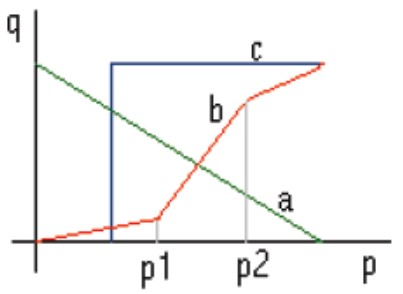
\includegraphics[width=5cm, keepaspectratio]{capitoli/immagini/imgs/elaborazioni_puntuali_immagine.jpg}
          \end{figure}

\end{itemize}

\subsection{Thresholding}

Consideriamo una funzione T a gradino, ottenendo così una
\textbf{elaborazione threshold (soglia)}.\\
Tale elaborazione fa sì che i valori dei pixel che non superano la
soglia fissata vengano portati a 0, mentre i valori dei pixel che
superano la soglia siano posti pari a 1.\\
Si produce così un'immagine \textbf{binaria}.

\begin{figure}[H]
    \centering
    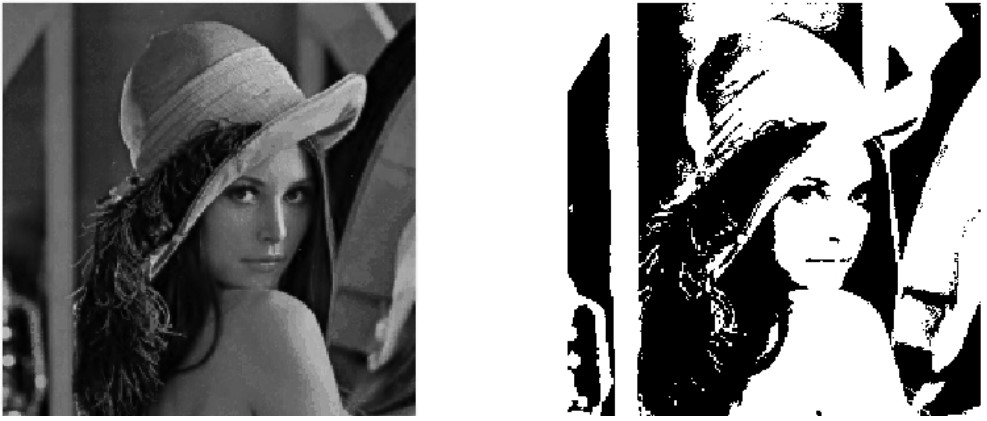
\includegraphics[width=10cm, keepaspectratio]{capitoli/immagini/imgs/foto_esempio_1.jpg}
\end{figure}

Questo è un tipico esempio di \textbf{binarizzazione}.
Si può ottenere una binarizzazione anche scegliendo una qualsiasi
altra \textbf{funzione di discriminazione}, invece di una soglia costante.

\subsection{Stiramento}

Consideriamo una $T$ del tipo:

\begin{figure}[H]
    \centering
    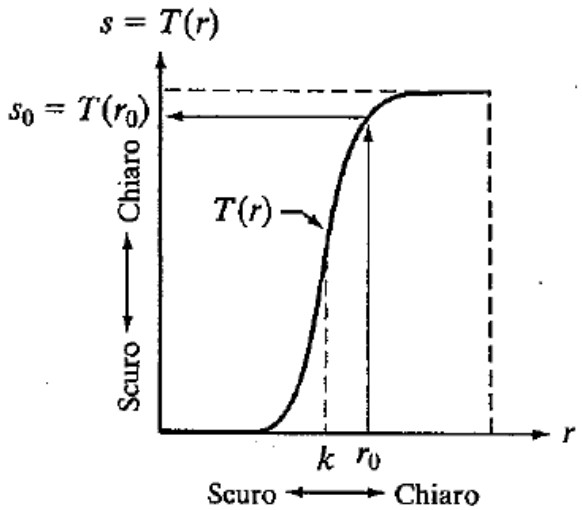
\includegraphics[width=6cm, keepaspectratio]{capitoli/immagini/imgs/trasformazione_esempio_2.jpg}
\end{figure}

Vengono scuriti i livelli di grigio al di sotto di $k$ e schiariti quelli al
di sopra di $k$. Si ottiene così uno \textbf{stiramento dell'immagine (image
    stretching)}. L'elaborazione threshold può essere riguardata come
caso limite di questo tipo di operazione.

\subsection{Negazione}

Consideriamo una $T$ del tipo:

$$
    T(r) = L - 1 - r
$$

se il range dinamico dell'immagine è $[0, L - 1]$
la scala di grigi viene invertita, ottenendo così una negazione.

\begin{figure}[H]
    \centering
    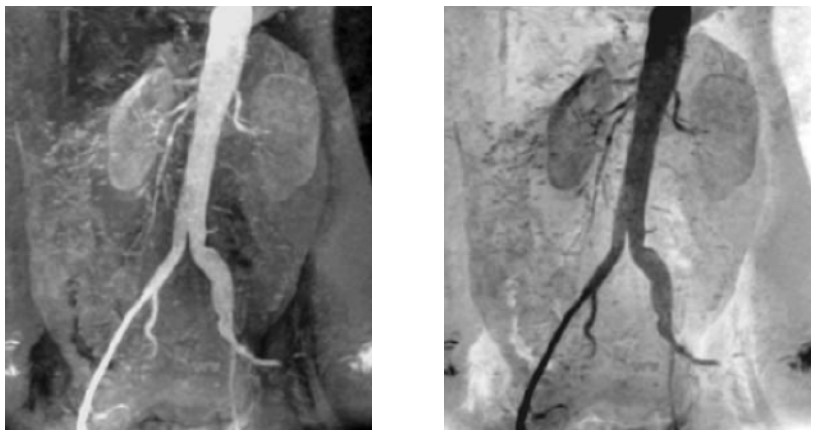
\includegraphics[width=8cm, keepaspectratio]{capitoli/immagini/imgs/angiografie_esempio_3.jpg}
\end{figure}

\subsection{Trasformazione Logaritmica}

Consideriamo una $T$ del tipo:

$$
    T(r) = c \log(1 + r), \ c \in  \mathbb{R}, r \geq 0
$$

che prende il nome di \textbf{trasformazione logaritmica}: associa ad una
stretta gamma di valori a bassa intensità dell'immagine originale
una più ampia gamma nell'immagine in output.\\
Per livelli ad alta intensità, invece, si verifica il contrario.\\
Un tipico caso in cui è utile applicare questa trasformazione è per
rappresentare la trasformata di Fourier, che spesso presenta una
gamma molto ampia di intensità, difficilmente riproducibile senza
perdere un significativo livello di dettaglio

\begin{figure}[H]
    \centering
    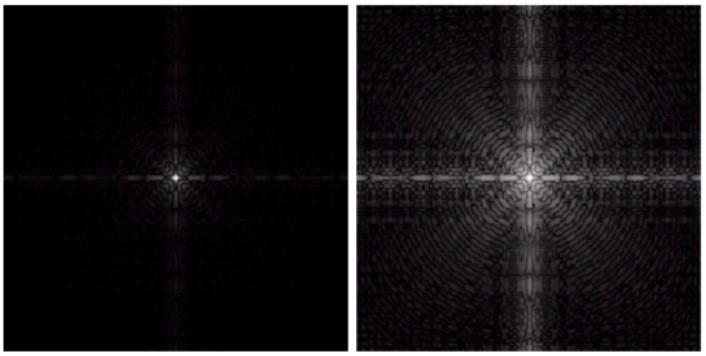
\includegraphics[width=10cm, keepaspectratio]{capitoli/immagini/imgs/trasformazione_logaritmica_esempio_4.jpg}
    \caption{Nella figura sinistra viene mostrato lo spettro di Fourier con valori in $[0, 1.5 \times 10^6]$. Mentre in quella di destra il risultato dell'applicazione della trasformazione logaritmica
        con $c = 1$ (valori in $[0, 6.2]$).
    }
\end{figure}

\subsection{Trasformazione di Potenza}

Consideriamo una $T$ del tipo:

$$
    T(r) = cr^\gamma, c, \gamma > 0,
$$

che prende il nome di \textbf{trasformazione di potenza (gamma)}
Se $\gamma < 1$ le curve potenza corrispondenti trasformano una stretta
gamma di valori scuri in una gamma più ampia di valori in output,
mentre se $\gamma > 1$, si verifica la trasformazione opposta.\\
La correzione tramite il fattore $\gamma$ è importante per la corretta
visualizzazione di immagini sullo schermo di un computer:
immagini non corrette nel modo giusto possono apparire sbiadite o,
al contrario, troppo scure.

\begin{figure}[H]
    \centering
    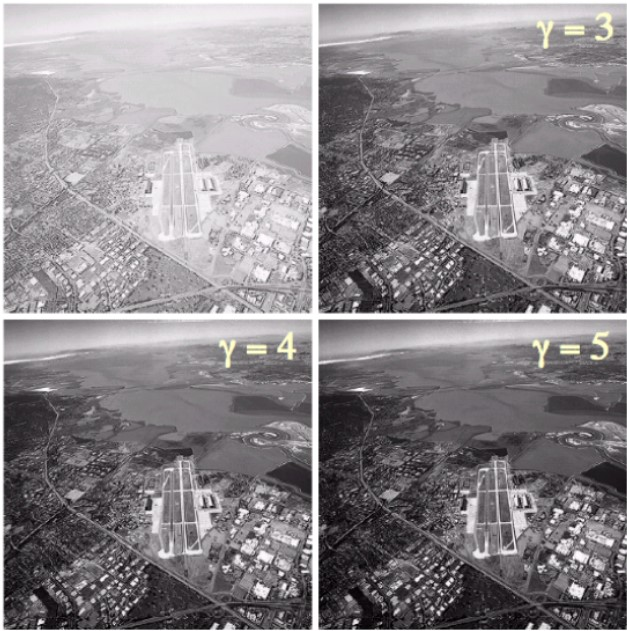
\includegraphics[width=6cm, keepaspectratio]{capitoli/immagini/imgs/foto_esempio_5.jpg}
\end{figure}

\subsection{Lineare a Tratti}

Considerando una $T$ \textbf{lineare a tratti} del tipo si ottiene uno
stretching del contrasto

\begin{figure}[H]
    \centering
    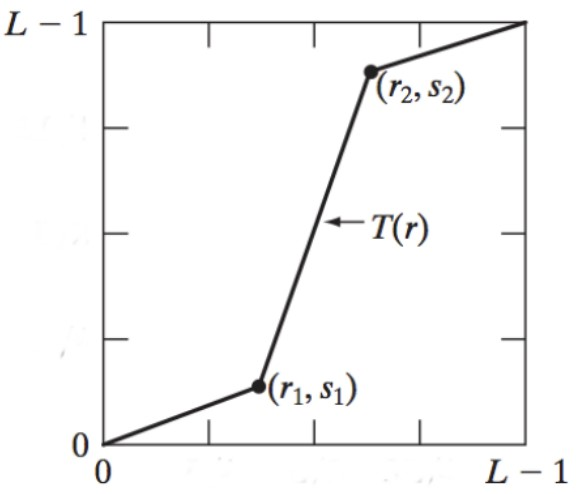
\includegraphics[width=5cm, keepaspectratio]{capitoli/immagini/imgs/lineare_a_tratti_esempio_6.jpg}
\end{figure}

In questo caso invece si ha uno stretching del contrasto differente perché si
sceglie come $(r_1, s_1) = (r_{min}, 0)$ e $(r_2, s_2) = (r_{max} , L - 1)$

\begin{figure}[H]
    \centering
    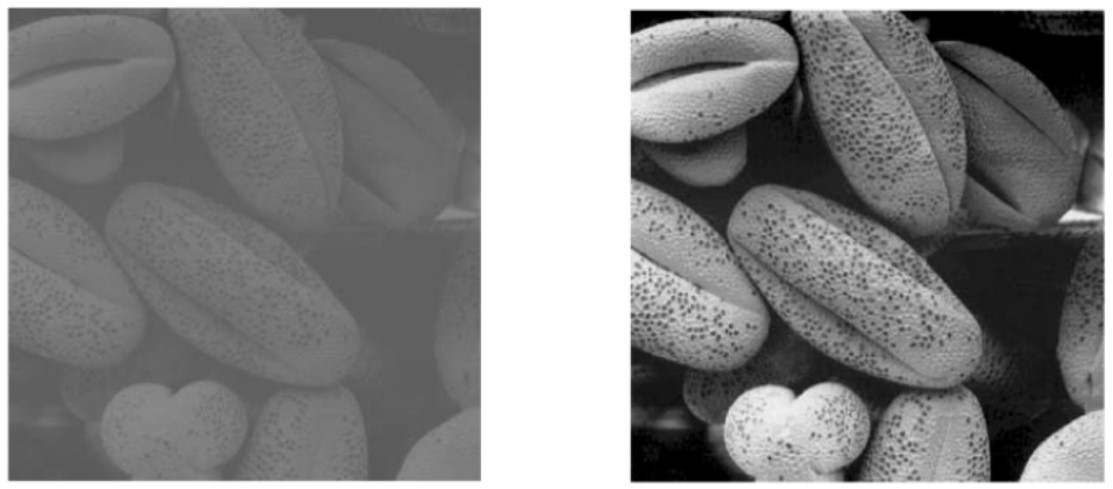
\includegraphics[width=10cm, keepaspectratio]{capitoli/immagini/imgs/globuli_rossi.jpg}
\end{figure}

\paragraph{Note:}
\begin{itemize}
    \item In questo caso $r_{min}$ e $r_{max}$ stanno ad indicare il più basso e alto valore
          nei livelli di grigio dell'immagine utilizzata.
\end{itemize}

\subsection{Altre Trasformazioni a Tratti}

\begin{figure}[H]
    \centering
    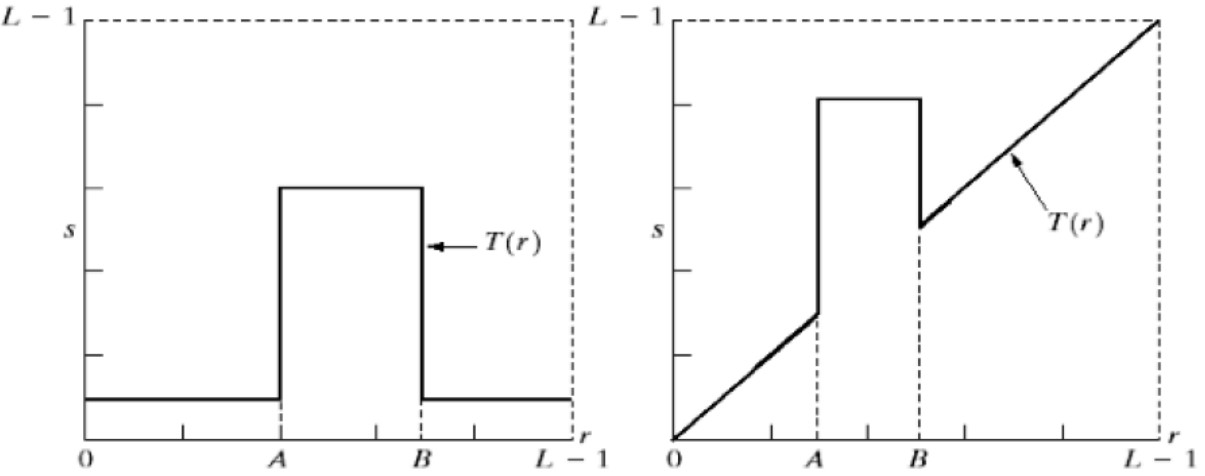
\includegraphics[width=\linewidth, keepaspectratio]{capitoli/immagini/imgs/trasformazioni_lineari_esempio_7.jpg}
\end{figure}

In questo caso prendiamo queste due diverse trasformazioni ed analizziamo il
loro effetto sull'immagine.

\begin{itemize}
    \item La prima crea una binarizzazione ma in questo caso utilizza due
          differenti gradazioni di grigio e sono precisamente bianco e nero.
    \item La seconda mette in \textbf{risalto} una porzione della scala di grigi
          alzandogli il livello e schiarendoli.
\end{itemize}

\begin{figure}[H]
    \centering
    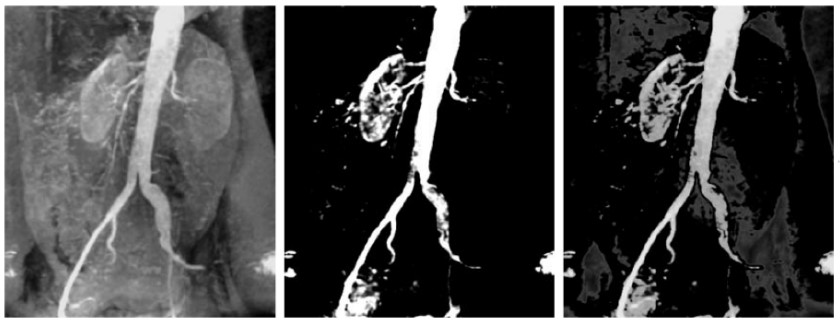
\includegraphics[width=\linewidth, keepaspectratio]{capitoli/immagini/imgs/angiografie_esempio_7.jpg}
\end{figure}

\begin{itemize}
    \item Nella prima immagine vediamo una normale Angiografia aortica.
    \item Nella seconda abbiamo il risultato della selezione di intensità del primo tipo (banda di
          interesse $[A, B]$ selezionata sulla parte alta della scala di grigi).
    \item Nella terza abbiamo il risultato della selezione di intensità del secondo tipo (banda
          $[A, B]$ sulle tonalità medio-grigie impostata sul nero, così da
          preservare le tonalità di grigio dei vasi e dei reni).
\end{itemize}

\subsection{Finestramento - Windowing}

\begin{definition}
    \textbf{Il windowing} consiste nel mostrare solo una parte del range dei valori di grigio dell'immagine.
\end{definition}

\begin{figure}[H]
    \centering
    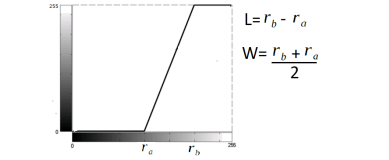
\includegraphics[width=\linewidth, keepaspectratio]{capitoli/immagini/imgs/win1.png}
\end{figure}

\textbf{Applicazione:} in molte immagini mediche il numero di valori della
scala dei grigi utili dal punto di vista diagnostico è sensibilmente
minore di tutti quelli disponibili. Usando sul monitor tutto il range
possibile si diminuisce il contrasto visibile nella zona di interesse.

\begin{figure}[H]
    \centering
    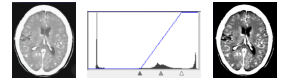
\includegraphics[width=\linewidth, keepaspectratio]{capitoli/immagini/imgs/windowing.png}
\end{figure}

\begin{itemize}
    \item Finestramento con $L = 169$ e $W = 97$
    \item Numero di grigio: $238$ (Immagine di sx) e $97$ (immagine di dx)
    \item Non viene aggiunta informazione, si aumenta solo il contrasto visibile
\end{itemize}

\section{Modelli delle Immagini}

In base al tipo di elaborazione che si vuole effettuare, può essere conveniente adottare diversi modelli per le immagini. Ad esempio:

\begin{itemize}
    \item \textbf{Modello Deterministico}
    \item \textbf{Modello Probabilistico}:
          \begin{itemize}
              \item sui \textbf{pixel} prevedendo che il loro valore sia
                    considerato una variabile aleatoria,
              \item sull'\textbf{immagine} riguardando cioè l'immagine stessa
                    come un processo stocastico

          \end{itemize}
\end{itemize}

\subsection{Il modello Probabilistico}

Nel modello probabilistico per i pixel, i valori assunti nei vari pixel ($N$ x
$M$) di un'immagine vengono considerati come valori assunti da una variabile
aleatoria in una successione di $N$ x $M$ esperimenti. Vado quini a modificare i
pixel in base ad un valore di probabilità. \\È dunque possibile analizzare ed
elaborare l'immagine utilizzando gli strumenti del calcolo delle probabilità e
del calcolo stocastico. Un esempio di questo processo è \textbf{l'analisi
    dell'istogramma}.

\subsubsection{L'istogramma dei toni di grigio}

\begin{definition}
    L'istogramma dei toni di grigio si ottiene contando, per ogni valore del
    codominio dell'immagine (spazio di tutti i valori che possono essere assunti
    dai pixel), il numero di volte che tale valore compare nell'immagine.
\end{definition}

Il grafico che si ricava è un istogramma, cioè un grafico a barre dove l'asse delle ascisse è suddiviso in tanti punti quanti sono i
possibili toni di grigio dell'immagine.\\

In termini probabilistici, l'istogramma rappresenta la distribuzione di probabilità della variabile
aleatoria $r$ ed indica il valore di grigio di un pixel, e quindi può essere visto come
la \textbf{carta d'identità di un'immagine}. Saper leggere l'istogramma ci
da un valore \textbf{qualitativo} dell'Immagine.

\begin{trivlist}
    \item \textbf{Esempio}: il codominio di un'immagine a 256 toni di grigio sarà formato da tutti i numeri interi da 0 a 255 $\rightarrow$ l'asse orizzontale sarà suddiviso in 256 parti.
\end{trivlist}

\begin{figure}[H]
    \centering
    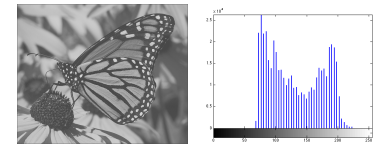
\includegraphics[width=\linewidth, keepaspectratio]{capitoli/immagini/imgs/esempio-istogramma.png}
\end{figure}

\begin{definition}
    In base alla definizione di distribuzione l'istogramma andrebbe normalizzato
    in modo da assumere valori tra 0 e 1. Se i toni di grigio sono $r_k$, $k =
        0, \ldots, 255$ allora l'altezza della barra in $r_k$ è pari alla frequenza
    relativa di $r_k$, ovvero:

    $$
        p(r_k) = \frac{n_k}{n}
    $$

    dove $n_k$ è il numero di pixel in cui viene assunto $r_k$, $n$ è il numero
    totale di pixel dell'immagine.
\end{definition}

L'istogramma quindi fornisce una raffigurazione sintetica del contenuto cromatico o di luminosità dell'immagine, dunque una descrizione
della qualità dell'immagine.

\begin{itemize}
    \item \textbf{Immagine troppo scura}
          la distribuzione è concentrata su toni bassi di grigio

          \begin{figure}[H]
              \centering
              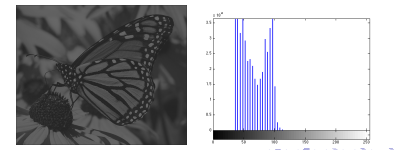
\includegraphics[width=\linewidth, keepaspectratio]{capitoli/immagini/imgs/isto-scuro.png}
          \end{figure}

    \item \textbf{Immagine troppo chiara}
          la distribuzione è concentrata su toni alti di grigio

          \begin{figure}[H]
              \centering
              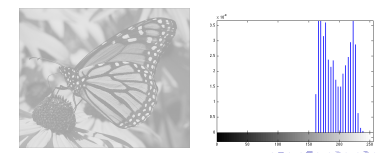
\includegraphics[width=\linewidth, keepaspectratio]{capitoli/immagini/imgs/isto-chiaro.png}
          \end{figure}

    \item \textbf{Immagine con alto contrasto}
          la distribuzione è concentrata su valori vicini a 0 e a 255. L'alto contrasto dell'immagine è quindi dovuto all'uniformità dell'istogramma.

          \begin{figure}[H]
              \centering
              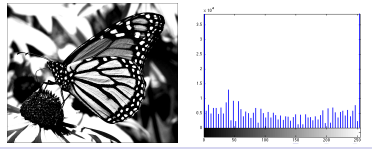
\includegraphics[width=\linewidth, keepaspectratio]{capitoli/immagini/imgs/alto-c.png}
          \end{figure}
\end{itemize}

\subsubsection{Interventi sull'istogramma}

Qualora le caratteristiche della distribuzione dei toni di grigio nell'immagine non siano ottimali, è consigliabile applicare
all'istogramma opportune trasformazioni, basate su sistemi stocastici.
\\Tra queste:

\paragraph{Equalizzazione dell'istogramma}

\begin{definition}
    Ha lo scopo di uniformare l'istogramma dell'immagine lungo tutto
    il suo dominio.
\end{definition}
Il risultato è un nuovo istogramma in cui il numero di pixel ad ogni
tono di grigio è il più possibile costante. \\\\
\textbf{Algoritmo:}

$$
    T(r_k) = (L-1)\sum_{j=0}^{k}p(r_j)=\frac{L-1}{n} \sum_{j=0}^{k}n_j = \frac{L-1}{MN}\sum_{j=0}^{k}n_j
$$

con $k=0,...,L-1$.
\\\\
\textbf{Il risultato} è l'aumento del contrasto.

\begin{figure}[H]
    \centering
    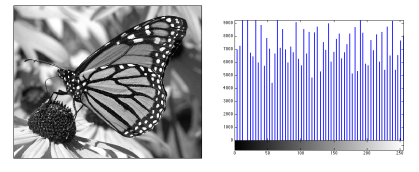
\includegraphics[width=\linewidth, keepaspectratio]{capitoli/immagini/imgs/eq-istogramma.png}
    \caption{L'immagine mostra il risultato dell'equalizzazione dell'istogramma.}
\end{figure}
\paragraph{Shift dell'istogramma}

\begin{definition}
    Lo Shift dell'istogramma consiste nel traslare i valori dell’istogramma.
\end{definition}
\textbf{Algoritmo:}

\begin{center}
    $T(r) = \alpha r$  $ \ \ \ \  0 < \alpha < 1$
    \\
    $T(r) = \alpha r + (L-1)(1-\alpha)$ $\ \ \ \ 0<\alpha<1$
\end{center}

Andrò quindi a shiftare verso sinistra o verso destra l'istogramma schiarendo o scurendo la mia immagine.
\\\\
Il \textbf{risultato} è un immagine più scura o schiarita.

\begin{figure}[H]
    \centering
    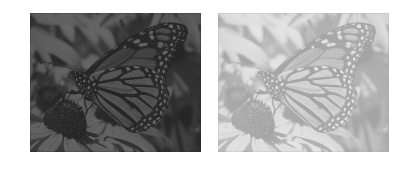
\includegraphics[width=\linewidth, keepaspectratio]{capitoli/immagini/imgs/shift-isto.png}
    \caption{L'immagine mostra il risultato dello Shift dell'isogramma.}
\end{figure}

\paragraph{Stretching dell'istogramma}

\begin{definition}
    Lo Stretching dell'istogramma consiste in uno $stiramento$ dell'istogramma, in modo da distanziarne i picchi.
\end{definition}

Si usa quando l'istogramma presenta dei picchi abbastanza ravvicinati, provocando un'immagine
piuttosto uniforme.
\\\\
\textbf{Algoritmo:}

$$
    T(r) =
    \begin{cases}
        0,                                         & 0 \le r \le r_{min}       \\
        (r - r_{min}) \frac{L-1}{r_{max}-r_{min}}, & r_{min} \le r \le r_{max} \\
        L-1,                                       & r_{max} \le r \le L-1
    \end{cases}
$$

dove $[r_{min}, r_{max} ]$ è il range osservato nell'immagine originale,
individuato dal minimo e dal massimo livello di grigio che presenta l'immagine.
\\Il risultato è \textbf{l'aumento di contrasto}

\begin{figure}[H]
    \centering
    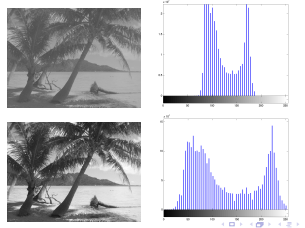
\includegraphics[width=\linewidth, keepaspectratio]{capitoli/immagini/imgs/stretch-isto.png}
\end{figure}

\section{Il Rumore}

\begin{definition}
    si intende l'insieme dei segnali indesiderati che si sovrappongono al segnale utile oggetto di studio (ad esempio un'immagine) causandone una degenerazione.
\end{definition}

Si possono avere diverse forme di degrado tra cui:
\begin{itemize}
    \item \textbf{Il rumore di quantizzazione}
    \item \textbf{Il rumore introdotto da condizioni esterne}
    \item \textbf{Il rumore introdotto dal sensore}
    \item \textbf{Il rumore introdotto dai dispositivi di
              amplificazione/condizionamento del segnale}
\end{itemize}

In base alle sue cause, il rumore si distingue tra:
\begin{itemize}
    \item \textbf{Rumore indipendente dal segnale} (additivo)
    \item \textbf{Rumore dipendente dal segnale} (la relazione tra il segnale
          corrotto e quello originale è non lineare)
\end{itemize}

\begin{trivlist}
    \item \textbf{Rumore indipendente dal segnale:} (caso più comune) la funzione
    che descrive il segnale corrotto è:

    $$
        f(x,y) = g(x,y)+v(x,y)
    $$
    dove $g(x,y)$ è il segnale e $v(x,y)$ è il rumore, che sarà di tipo
    \textbf{additivo}

    \item \textbf{Rumore dipendente dal segnale:} l'intensità del rumore dipende
    dal segnale. Supponendo anche che esso sia molto più grande del segnale, la
    funzione è

    $$
        f(x,y)=g(x,y)+v(x,y)g(x,y)=g(x,y)(1+v(x,y)) \approx g(x,y)v(x,y)
    $$

    dove $g(x,y)$ è il segnale e $v(x,y)$ è il rumore, che sarà di tipo
    \textbf{moltiplicativo}
\end{trivlist}

Essendo di natura intrinsecamente stocastica, il rumore viene in genere analizzato usando la teoria dei processi stocastici ed è
caratterizzato in base alla:

\begin{itemize}
    \item \textbf{Distribuzione:} descrive la probabilità che il rumore assuma
          certi valori di intensità
    \item \textbf{Distribuzione spettrale:} ha a che fare con l'energia ad esso
          associata, al variare della frequenza
\end{itemize}

\subsection{Il modello del rumore}

Per poter caratterizzare e studiare il rumore in un'immagine si fanno in genere delle ipotesi semplificative, in modo che il rumore abbia una qualche distribuzione di probabilità: si costruisce in
questo modo un modello del rumore.
\\Una modellizzazione tipica prevede che:

\begin{itemize}
    \item \textbf{lo spettro abbia distribuzione uniforme (rumore bianco)}
    \item \textbf{il rumore abbia distribuzione gaussiana, cioè}
          \begin{equation*}
              p(r)=\frac{1}{\sigma \sqrt{2 \pi}}e^{-\frac{(r-\mu)^2}{2\sigma^2}}
              \qquad
              \begin{gathered}
                  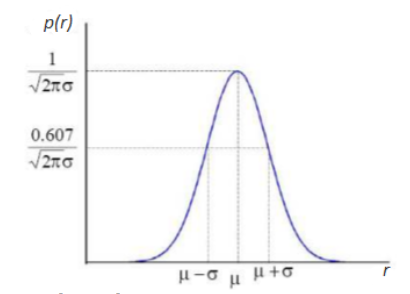
\includegraphics[width=6cm, keepaspectratio]{capitoli/immagini/imgs/campana.png}
              \end{gathered}
          \end{equation*}
          dove $\mu$ è il valor medio e $\sigma$ la deviazione standard.
\end{itemize}

\begin{figure}[H]
    \centering
    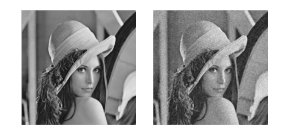
\includegraphics[width=8cm, keepaspectratio]{capitoli/immagini/imgs/esempio-rumore.png}
    \caption{Immagine originale e immagine corrotta da rumore gaussiano}
\end{figure}

\subsubsection{Il rumore Salt and Pepper}

Nel caso in cui il rumore abbia distribuzione spaziale di tipo impulsivo, si
parla di rumore salt and pepper (sale e pepe): agisce corrompendo in maniera
casuale i pixel dell'immagine, portandone il valore a $0$ (valore minimo)
oppure a $255$ (valore massimo).

\begin{equation*}
    p(r) = \begin{cases}
        p_a, & r = 0      \\
        p_b, & r = 255    \\
        0,   & altrimenti
    \end{cases}
    \qquad
    \begin{gathered}
        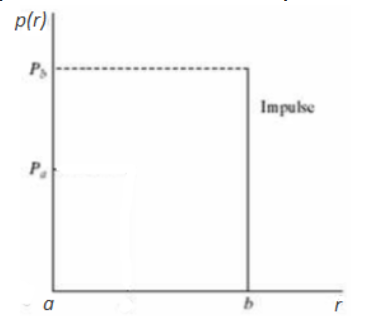
\includegraphics[width=6cm, keepaspectratio]{capitoli/immagini/imgs/salepepe.png}
    \end{gathered}
\end{equation*}

Ovviamente il rumore impulsivo, pur essendo additivo, \textbf{non è
    lineare.}

\begin{figure}[H]
    \centering
    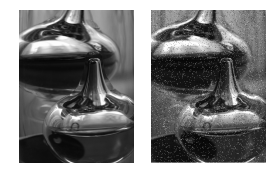
\includegraphics[width=10cm, keepaspectratio]{capitoli/immagini/imgs/esempio-salt-pepper.png}
    \caption{Immagine originale e immagine corrotta da rumore salt and pepper}
\end{figure}

\subsubsection{Rumore di Rayleigh}
Distribuzione del \textbf{rumore di Rayleigh}

\begin{equation*}
    p(r) = \begin{cases}
        \frac{2}{b}(r-a)e^{-{r-a}\frac{2}{b}}, & r \ge a \\
        0,                                     & r<a
    \end{cases}
    \qquad
    \begin{gathered}
        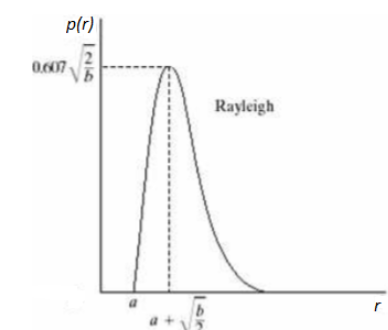
\includegraphics[width=6cm, keepaspectratio]{capitoli/immagini/imgs/raley.png}
    \end{gathered}
\end{equation*}

dove il valor medio e la deviazione standard sono dati da:

$$
    \mu = a + \sqrt{\pi b/4} \ \sigma = \sqrt{\frac{b(4-\pi)}{4}}
$$

Nel grafico lo scostamento dall'origine e la forma inclinata verso
destra rende questa densità utile per l'approssimazione di
istogrammi non simmetrici e può essere utilizzata per rappresentare
fenomeni di rumori tipici di alcuni sensori di range.

\begin{figure}[H]
    \centering
    
\includegraphics[width=8cm, keepaspectratio]{capitoli/immagini/imgs/rumore_raeli.png}
    \caption{Immagine originale e immagine corrotta da rumore Rayleigh}
\end{figure}

\subsubsection{Rumore Gamma}

Distribuzione del \textbf{rumore gamma}:

\begin{equation*}
    p(r) = \begin{cases}
        \frac{a^b r^{b-1}}{(b-1)!}e^-{ar}, & r \ge a \\
        0,                                 & r<a
    \end{cases}
    \qquad
    \begin{gathered}
        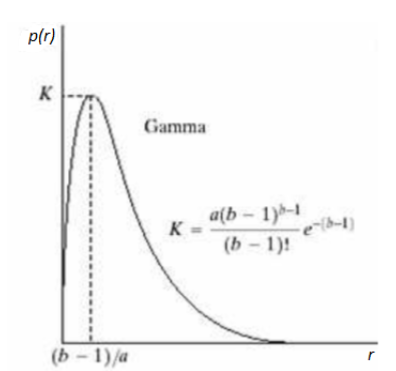
\includegraphics[width=6cm, keepaspectratio]{capitoli/immagini/imgs/gamma.png}
    \end{gathered}
\end{equation*}

dove $a > 0$, $b$ è un intero positivo e il valor medio e la deviazione standard sono dati da:

\begin{center}
    $\mu=\frac{b}{a}$ $\sigma=\frac{\sqrt{b}}{a}$
\end{center}

Questo rumore è presente nelle immagini laser.

\begin{figure}[H]
    \centering
    
\includegraphics[width=8cm, keepaspectratio]{capitoli/immagini/imgs/rumore_gamma.png}
    \caption{Immagine originale e immagine corrotta da rumore Gamma}
\end{figure}

\subsubsection{Rumore Esponenziale}

Distribuzione del \textbf{rumore Esponenziale}:

\begin{equation*}
    p(r) = \begin{cases}
        ae^{-ar}, & r \ge a \\
        0,        & r<0
    \end{cases}
    \qquad
    \begin{gathered}
        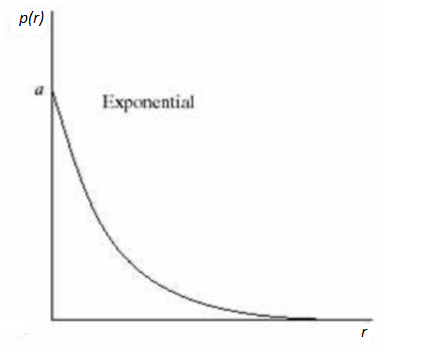
\includegraphics[width=6cm, keepaspectratio]{capitoli/immagini/imgs/esponenziale.png}
    \end{gathered}
\end{equation*}

dove $a > 0$, b e il valor medio e la deviazione standard sono dati da:

$$
    \mu = \frac{1}{a} \ \ \sigma = \frac{1}{a}
$$

Questo rumore è un caso particolare del rumore di Gamma con $b = 1$.


\begin{figure}[H]
    \centering
    
\includegraphics[width=8cm, keepaspectratio]{capitoli/immagini/imgs/esempio-esponenziale.png}
    \caption{Immagine originale e immagine corrotta da rumore Esponenziale}
\end{figure}

\subsection{Signal-Noise Ratio}

Per avere una valutazione numerica dell'entità del rumore associato ad una data immagine si può ricorrere al \textbf{rapporto segnale-rumore
    (Signal Noise Ratio - SNR)}, definito come:

\begin{center}
    $
        SNR = \frac{\sum_{(x,y)}^{}f^2(x,y)}{\sum_{(x,y)}^{}v^2(x,y)}
    $
\end{center}

dove $f(x, y)$ è l'intensità del pixel $(x, y)$ dell'immagine (già corrotta dal rumore), $v(x, y)$ è il rumore e le sommatorie sono al
variare di tutti i pixel $(x, y)$ dell'immagine.

\section{Filtri}

\begin{definition}
    Il rumore può essere corretto applicando opportune trasformazioni ai pixel dell'immagine, dette filtri.
\end{definition}
Per ogni tipo di rumore esiste un filtraggio differente, che risulterà il più
adatto ad attenuare o eliminare quel particolare rumore. In genere, la scelta
del filtro dipende dalla linearità o meno della relazione fra l'immagine
corrotta e quella originale. È possibile combinare più filtri, in modo da avere
effetti più complessi.

\subsection{Il filtraggio spaziale}

Un filtro spaziale è caratterizzato da:

\begin{itemize}
    \item Un intorno (\textbf{maschera}), in genere di dimensioni dispari;
    \item Un'operazione predefinita che viene applicata ai pixel nell'intorno
\end{itemize}
se l'operazione è lineare si parla di \textbf{filtro lineare}.
\\\\
L'intensità dell'immagine filtrata nel pixel (x,y) sarà:

\begin{center}
    $g(x,y) = \sum_{s=-a}^{a}\sum_{t=-b}^{b}w(s,t)f(x+s,y+t)$,
\end{center}

con $x=0,..,M-1$, $y=0,...,N-1$ (\textbf{correlazione di f e w}), dove i valori $w$ sono i \textbf{coefficienti della maschera}
avente dimensione $m$ x $n$, con $m = 2a+1$ e $n = 2b+1$
\\\\
Ad esempio, se la maschera ha dimensione 3 x 3, l'intensità dell'immagine filtrata nel pixel ($x,y$) sarà:
\begin{itemize}
    \item $g(x,y)=w(-1,-1)f(x-1,y-1)+w(-1,0)f(x-1,y)+...+w(0,0)f(x,y)+...+w(1,1)f(x+1,y+1)$
\end{itemize}

\subsection{Filtri lineari}

I filtri maggiormente utilizzati per la rimozione del rumore sono i cosiddetti
\textbf{filtri di smoothing}, i quali eliminano picchi e increspature
(passa-basso).

\subsubsection{Filtro medio}
Il filtro medio sostituisce il valore di ogni pixel prefissato con il
valor medio dei pixel in un suo intorno di dimensioni fissate.

\[
    \frac{1}{mn} \times
    \begin{bmatrix}
        1      & \ldots & 1      \\
        \vdots & \ddots & \vdots \\
        1      & \ldots & 1
    \end{bmatrix}
\]

Il \textbf{filtro medio} è molto utilizzato ad esempio per correggere il
\textbf{rumore gaussiano.}

\begin{figure}[H]
    \centering
    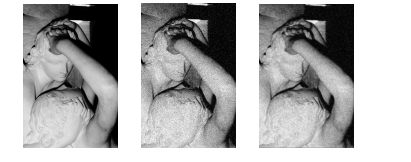
\includegraphics[width=\linewidth, keepaspectratio]{capitoli/immagini/imgs/filtro-medio-esempio2.png}
    \caption{Immagine originale, immagine corrotta da rumore gaussiano e immagine filtrata con filtro medio}
\end{figure}

\subsubsection{Filtro di media ponderata}
Il filtro media ponderata sostituisce il valore di ogni pixel prefissato con la media ponderata dei pixel in un suo
intorno di dimensioni fissate.

\begin{center}
    $g(x,y)=\frac{\sum_{s=-a}^{a}\sum_{t=-b}^{b}w(s,t)f(x+s,y+t)}{\sum_{s=-a}^{a}\sum_{t=-b}^{b}w(s,t)}$
\end{center}

\subsubsection{Filtro Gaussiano}
Il filtro gaussiano: sostituisce al valore di ogni pixel prefissato la
media pesata dei valori dei pixel in un suo intorno. I pesi sono distribuiti secondo una funzione gaussiana.

\[
    \frac{1}{16} \times
    \begin{bmatrix}
        1 & 2 & 1 \\
        2 & 4 & 2 \\
        1 & 2 & 1
    \end{bmatrix}
\]

\begin{figure}[H]
    \centering
    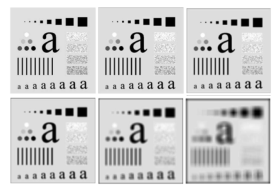
\includegraphics[width=10cm, keepaspectratio]{capitoli/immagini/imgs/filtri-l-esempio.png}
    \caption{Possiamo vedere l'applicazione della sfocatura con filtro medio
        tramite maschere di dimensioni 3, 5, 9, 15, 35 su un immagine di $500 \times 500$ pixel.}
\end{figure}

\subsection{Filtri non lineari}
I rumori non lineari (ad esempio quello impulsivo) non possono essere corretti con i filtri lineari.
Possono essere trattati invece efficacemente con \textbf{filtri non lineari}
\subsubsection{Filtro mediano}
Il filtro Mediano sostituisce al valore di ogni pixel prefissato la
mediana (valore centrale della lista ordinata) dei
valori dei pixel nell'intorno fissato.

Il filtro mediano risulta particolarmente adatto a correggere il rumore \textbf{salt and pepper}, a differenza del filtro medio che, come si
vede dall'esempio seguente, non risulta invece particolarmente efficace.

\begin{figure}[H]
    \centering
    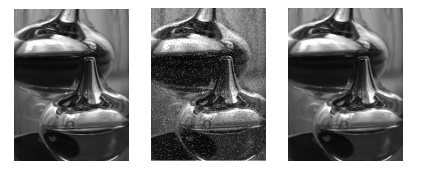
\includegraphics[keepaspectratio]{capitoli/immagini/imgs/esempio-filtro-mediano.png}
    \caption{Immagine originale, immagine corrotta da rumore \textbf{salt and pepper} e immagine filtrata con \textbf{filtro mediano}}
\end{figure}
\begin{figure}[H]
    \centering
    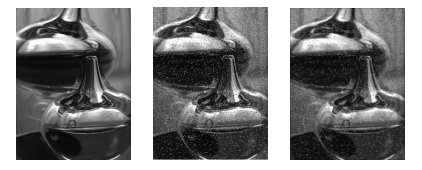
\includegraphics[keepaspectratio]{capitoli/immagini/imgs/esempio-filtro-medio.png}
    \caption{Immagine originale, immagine corrotta da rumore \textbf{salt and pepper} e immagine filtrata con \textbf{filtro medio}}
\end{figure}

\subsubsection{Filtro di massimo}

Sia $S_p$ una maschera di dimensioni $m $ x $n$, dove $p = (x,y)$ è il pixel centrale della maschera.
Il filtro di massimo sostituisce a p il massimo dei valori dei pixel in $S_p$, cioè

$$
    g_{max}(x,y)= \max_{(x,y) \in S_p} f(x,y)
$$

Questo filtro è utile per \textbf{diminuire il rumore di tipo "pepper"}.

\subsubsection{Filtro di minimo}

Il \textbf{filtro di minimo} sostituisce a $p$ il minimo dei valori dei pixel in $S_p$ cioè:

$$
    g_{min}(x,y) = \min_{(x,y) \in S_p} f(x,y)
$$

Questo filtro è utile \textbf{per diminuire il rumore di tipo "salt"}

\subsubsection{Filtro di Punto Medio}

Il filtro di punto medio sostituisce a $p$ il punto medio tra il massimo ed il minimo
dei valori dei pixel in $S_p$, cioè

$$
    g(x,y) = \frac{1}{2} \left[\max_{(x,y) \in S_p} f(x) + \min_{(x,y) \in S_p} f(x)\right]
$$

\subsubsection{Filtro medio alpha-trimmed}

Fissato un valore $0 \le d \le mn - 1$, supponiamo di cancellare in $S_p$ i $d/2$ valori più chiari e i $d/2$ valori più scuri; delle
restanti intensità ne calcoliamo la media aritmetica, cioè:

$$
    g(x,y) = \frac{1}{mn-d} \sum_{(x,y) \in \bar{S_p}} f(x,y)
$$

dove $\bar{S_p}$ è l'insieme dei pixel $S_p$ rimanenti.
Questo filtro risulta utile in situazioni in cui \textbf{si sovrappongono diversi tipi di rumore}, ad esempio nel caso di una combinazione tra
rumore salt an pepper e rumore gaussiano.

\section{Filtri di Sharpening}

L'obiettivo di questi filtri è quello di \textbf{marcare i bordi (edge
    detection)}, attribuendo meno importanza alle aree che hanno variazione lenta a
livello di intensità. Si basano sull'operatore di derivazione ed hanno l'effetto
di evidenziare soltanto i bordi dell'immagine. In forma discreta, se $f$
rappresenta l'intensità associata a ogni pixel $(x,y)$, le derivate possono
essere espresse come differenze finite:

\begin{center}
    $\frac{\partial{f}}{\partial{x}}(x,y) \sim f(x+1, y) - f(x, y)$, $\frac{\partial{f}}{\partial{y}}(x,y) \sim f(x,y+1) - f(x,y)$
    \\
    $\frac{\partial{f^2}}{\partial{x^2}}(x,y) \sim f(x+1,y) + f(x-1, y) - 2f(x,y)$
    \\
    $\frac{\partial{f^2}}{\partial{y^2}}(x,y) \sim f(x,y+1) + f(x, y-1) - 2f(x,y)$
\end{center}

Il filtro di sharpening ha l'effetto di evidenziare soltanto i bordi dell'immagine.
\begin{figure}[H]
    \centering
    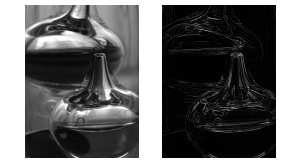
\includegraphics[width=8cm, keepaspectratio]{capitoli/immagini/imgs/sharpening.png}
    \caption{Applicazione di un filtro di sharpening}
\end{figure}

\TODO[inline]{Da ricontrollare e aggiungere spiegazioni}
\begin{figure}[H]
    \centering
    \includegraphics[width=11cm, keepaspectratio]{capitoli/immagini/imgs/sharpering2.png}
\end{figure}

\subsection{Filtro del Gradiente}

Operatore Gradiente:

\begin{center}
    $\nabla f=(\frac{\partial{f}}{\partial{x}}, \frac{\partial{f}}{\partial{y}})$,
\end{center}

Una comune implementazione della derivata prima nell'ambito dell'image processing è costituita dal modulo del gradiente

\begin{center}
    $| \nabla f(x,y) |$ $\sim$ $|\frac{\partial{f}}{\partial{x}}|$ $+$ $|\frac{\partial{f}}{\partial{y}}|$
\end{center}

Maschere:

\begin{center}
    \[
        \begin{bmatrix}
            0 & 0  & 0 \\
            0 & -1 & 0 \\
            0 & 1  & 0
        \end{bmatrix}
        \begin{bmatrix}
            0 & 0  & 0 \\
            0 & -1 & 1 \\
            0 & 0  & 0
        \end{bmatrix}
    \]
\end{center}

\begin{figure}[H]
    \centering
    \includegraphics[width=8cm, keepaspectratio]{capitoli/immagini/imgs/gradiente.png}
    \caption{Applicazione del Filtro del Gradiente}
\end{figure}

\subsection{Filtro di Sobel}
Un'altra approssimazione discreta del gradiente è data da:

\begin{align*}
    \nabla f(x,y) & \sim \frac{\partial{f}}{\partial{x}} + \frac{\partial{f}}{\partial{y}} \sim \\
                  & \sim  |[f(x+1,y-1) + 2f(x+1,y) + f(x+1 y+1)]  \ +                           \\
                  & - |[f(x-1, y-1)+2f(x-1,y) + f(x-1, y+1)]|     \ +                           \\
                  & + |[f(x-1, y+1) + 2f(x,y+1)+f(x+1,y+1)]       \ +                           \\
                  & - [f(x-1,y -1) + 2f(x,y-1) + f(x+1,y-1)]|
\end{align*}

Maschere:

\begin{center}
    \[
        \begin{bmatrix}
            -1 & -2 & -1 \\
            0  & 0  & 0  \\
            1  & 2  & 1
        \end{bmatrix}
        \begin{bmatrix}
            -1 & 0 & 1 \\
            -2 & 0 & 2 \\
            -1 & 0 & 1
        \end{bmatrix}
    \]
\end{center}

che sono detti \textbf{operatori di Sobel.}

\begin{figure}[H]
    \centering
    \includegraphics[width=8cm, keepaspectratio]{capitoli/immagini/imgs/sobel.png}
    \caption{Immagine originale e immagine filtrata tramite il gradiente di Sobel.}
\end{figure}

\subsection{Filtro di Prewitt}
Analogo a quello di Sobel eccetto per le maschere di convoluzione
che in questo caso sono:
\begin{center}
    \[
        \begin{bmatrix}
            -1 & 0 & 1 \\
            -1 & 0 & 1 \\
            -1 & 0 & 1
        \end{bmatrix}
        \begin{bmatrix}
            -1 & -1 & -1 \\
            0  & 0  & 0  \\
            1  & 1  & 1
        \end{bmatrix}
    \]
\end{center}


\begin{figure}[H]
    \centering
    \includegraphics[width=8cm, keepaspectratio]{capitoli/immagini/imgs/prewitt.png}
    \caption{Immagine originale e immagine filtrata tramite il gradiente
        di Prewitt.}
\end{figure}

\subsection{Filtro di Roberts}
Si ottiene mediante la seguente approssimazione del gradiente:

\begin{align*}
    |\nabla f(x,y)| & \sim |\frac{\partial{f}}{\partial{x}}| + |\frac{\partial{f}}{\partial{y}}| \sim \\
                    & \sim |f(x,y) - f(x+1, y+1)| + |f(x+1, y) - f(x,y+1)|
\end{align*}

Calcola il gradiente lungo le direzioni diagonali.
\\\\
Maschere:

\begin{center}
    \[
        \begin{bmatrix}
            0 & 0 & 0  \\
            0 & 1 & 0  \\
            0 & 0 & -1
        \end{bmatrix}
        \begin{bmatrix}
            0 & 0 & 0  \\
            0 & 0 & -1 \\
            0 & 1 & 0
        \end{bmatrix}
    \]
\end{center}

\begin{figure}[H]
    \centering
    \includegraphics[width=10cm, keepaspectratio]{capitoli/immagini/imgs/roberts.png}
    \caption{Nella figura possiamo osservare l'applicazione delle singole matrici $\nabla x$, $\nabla y$ e poi l'applicazione di tutte e due in contemporanea (filtro di Roberts).}
\end{figure}

\subsection{Filtro Laplaciano}

Operatore Laplaciano:

\begin{align*}
    \nabla^2 f & = \frac{\partial^2{f}}{\partial{x^2}} + \frac{\partial^2{f}}{\partial{y^2}} \sim \\
               & \sim f(x+1,y)+f(x-1,y)+f(x,y+1)+f(x,y-1)-4f(x,y)
\end{align*}

Maschera:

\begin{center}
    \[
        \begin{bmatrix}
            0 & 1  & 0 \\
            1 & -4 & 1 \\
            0 & 1  & 0
        \end{bmatrix}
    \]
\end{center}

oppure, tenendo conto delle direzioni diagonali:

\begin{center}
    \[
        \begin{bmatrix}
            1 & 1  & 1 \\
            1 & -8 & 1 \\
            1 & 1  & 1
        \end{bmatrix}
    \]
\end{center}

\begin{figure}[H]
    \centering
    \includegraphics[width=8cm, keepaspectratio]{capitoli/immagini/imgs/laplaciano.png}
    \caption{(a) Immagine originale, (b) con laplaciano, (c) con laplaciano con
        diagonali.}
\end{figure}

\subsection{Filtro Differenziale}

Sfrutta la proprietà di attraversamento dello zero della derivata seconda nelle varie direzioni, coordinate e diagonali, che ha come effetto quello di evidenziare direzionalmente i bordi di un'immagine lungo di esse.
\\Dalle approssimazioni:

\begin{align*}
    \frac{\partial^2{f}}{\partial{x}^2}(x,y) & \sim f(x+1,y)+f(x-1,y)-2f(x,y),                                \\
    \frac{\partial^2{f}}{\partial{y}^2}(x,y) & \sim f(x,y+1)+f(x,y-1)-2f(x,y),                                \\
    \frac{\partial^2{f}}{\partial{x,y}}(x,y) & \sim \frac{1}{4}[f(x-1,y-1)-f(x-1,y+1)-f(x+1,y-1)+f(x+1, y+1)]
\end{align*}

Si ottengono le maschere:
\begin{center}
    \[
        \begin{bmatrix}
            0 & 1  & 0 \\
            0 & -2 & 0 \\
            0 & 1  & 0
        \end{bmatrix}
        \begin{bmatrix}
            0 & 0  & 0 \\
            1 & -2 & 1 \\
            0 & 0  & 0
        \end{bmatrix}
        \begin{bmatrix}
            \frac{1}{4}  & 0 & -\frac{1}{4} \\
            0            & 0 & 0            \\
            -\frac{1}{4} & 0 & \frac{1}{4}
        \end{bmatrix}
    \]
\end{center}

\begin{figure}[H]
    \centering
    \includegraphics[width=8cm, keepaspectratio]{capitoli/immagini/imgs/digital-composing.png}
    \caption{Possiamo utilizzare il filtro differenziale per effettuare il Digital Compositing.}
\end{figure}

\section{Operazioni aritmetiche e Image Enhancement}

Date due immagini digitali $f(x,y)$ e $g(x,y)$ della stessa dimensione, si
possono definire le seguenti operazioni:

% \begin{align*}
%     s(x,y) = f(x,y) + g(x,y),
%     t(x,y) = f(x,y)-g(x,y),
%     p(x,y)=f(x,y) \cdot g(x,y),
%     d(x,y) = f(x,y)/g(x,y), (g(x,y) \neq 0, \forall(x,y)).
% \end{align*}

\begin{itemize}
    \item \textbf{Sommatoria di immagini:}
          date due immagini è possibile definire la loro somma come:

          $$
              s(x,y) = f(x,y) + g(x,y)
          $$

          Questa operazione è utile per effettuare l'enhancement con
          un'operazione di sommatoria.\\

          Siano $g_i(x,y)$ $K$ immagini corrotte da rumore additivo $\eta_i$ (eta),
          ovvero

          $$
              g_i(x,y) = f(x,y) + \eta_i(x,y), \ i=...K,
          $$

          dove $f(x,y)$ è l'immagine priva di rumore.\\
          Se $\bar{g}(x,y)$ è la loro media, ovvero

          $$
              \bar{g}(x,y)=\frac{1}{K} \sum_{i=1}^{K}g_i(x,y)
          $$

          allora sotto opportune ipotesi, risultata:

          $$
              E\left[\bar{g}(x,y)\right] = f(x,y) \ \text{ e } \ \sigma^2_{\bar{g}(x,y)}=\frac{1}{K}\sigma^2_{\eta(x,y)}
          $$

          \begin{figure}[H]
              \centering
              \includegraphics[width=10cm, keepaspectratio]{capitoli/immagini/imgs/sommatoria-immagini.png}
              \caption{a) Immagine originale affetta da rumore gaussiano
                  b)-f) Risultato della media di 5, 10, 20, 50 e 100 immagini
                  rumorose.}
          \end{figure}

    \item \textbf{Sottrazione di immagini}

          $$
              g(x,y) = f(x,y)-h(x,y)
          $$

          Si utilizza, ad esempio, quando si vogliono evidenziare le differenze
          fra due immagini, dove $h(x,y)$, detta maschera, è un'immagine della
          regione di interesse. Un esempio è la \textbf{Digital
              Subtraction Angiography (DSA)}.
          \begin{figure}[H]
              \centering
              \includegraphics[width=10cm, keepaspectratio]{capitoli/immagini/imgs/sottrazione.png}
          \end{figure}

    \item \textbf{Moltiplicazione e divisione di immagini}
          \TODO[inline]{Ricontrollare ed ampliare!}
          $$
              g(x,y) = f(x,y) \cdot h(x,y)
          $$
          \textbf{Esempi:}
          \begin{itemize}
              \item Correzzione dell'ombreggiatura(shading)
              \item Selezione di una ROI (Region of Interest)
          \end{itemize}

          \begin{figure}[H]
              \centering
              \includegraphics[width=10cm, keepaspectratio]{capitoli/immagini/imgs/moltiplicazione.png}
          \end{figure}
\end{itemize}


\chapter{Image Segmentation}

La segmentazione di un'immagine nell'elaborazione digitale è un processo di
partizione dell'immagine in regioni significative.

\begin{definition}
    E' il processo con il quale si classificano i pixel dell'immagine che hanno caratteristiche comuni: pertanto ciascun pixel in una regione
    è simile agli altri della stessa regione per una qualche proprietà o caratteristica (colore, intensità o texture).
\end{definition}

Matematicamente, il processo di segmentazione di un'immagine $f(x,y)$ in regioni
$R_1,...,R_n$ deve soddisfare le seguenti condizioni:

\begin{itemize}
    \item $\cup^n_{i=1}$ $R_i = f(x,y)$
    \item Ogni regione $R_i$ con $i=1,...,n$ è connessa;
    \item $R_i \cap R_j = \emptyset$ con $i \neq j$;
    \item Se $P(\cdot)$ è un predicato che indica la conformità di tutti i pixel
          di una regione $R_i$ ad un particolare modello della regione
          stessa, allora devono valere:
          \begin{itemize}
              \item $P(R_i) = vero$ $\forall i = 1...n$
              \item $P(R_i \cup R_j) = falso$ $\forall R_i, R_j$ regioni adiacenti
          \end{itemize}
\end{itemize}

La segmentazione dell'immagine ha molte applicazioni:

\TODO[inline]{Riorganizzare la visualizzazione delle immagini!}

\begin{figure}[H]
    \centering
    \includegraphics[width=9cm, keepaspectratio]{capitoli/immagini/imgs/biologia.png}
    \caption{Biologia}
\end{figure}

\begin{figure}[H]
    \centering
    \includegraphics[width=9cm, keepaspectratio]{capitoli/immagini/imgs/texture.png}
    \caption{Texture}
\end{figure}

\begin{figure}[H]
    \centering
    \includegraphics[width=6cm, keepaspectratio]{capitoli/immagini/imgs/medicina.png}
    \caption{Medicina}
\end{figure}


Le fondamentali metodologie di segmentazione sono:
\begin{itemize}
    \item \textbf{Thresholding Segmentation:} segmentazione mediante
          sogliatura;
    \item \textbf{Edge Segmentation:} edge based segmentation - localizzazione
          dei bordi;
    \item \textbf{Region Based Segmentation:} operatori morfologici;
    \item \textbf{Clustering Based Segmentation:} raggruppamento di oggetti
          sulla base della loro distanza reciproca;
    \item \textbf{Matching Techniques:} tecniche basate sulla conoscenza a
          priori.
\end{itemize}

\section{Thresholding Based Segmentation}

Singoli pixel dell'immagine sono catalogati come "pixel oggetto" se il loro
valore è maggiore di una certa soglia e come "pixel di sfondo" se il valore è
sotto la soglia. L'immagine binaria in uscita ha valore pari a 1 per ogni pixel
dell'oggetto e pari a 0 per lo sfondo.

\begin{trivlist}
    \item \textbf{Problema:} individuare il valore ottimo che minimizza l'errore dovuto all'oversegmentation (troppi oggetti) e
    all'undersegmentation (pochi oggetti).
    \item \textbf{Soluzione:} sogliatura locale $\rightarrow$ scelta di un valore di soglia diverso,
    adatto ad ogni regione esaminata.
\end{trivlist}

\subsection{Thresholding manuale}
\begin{itemize}
    \item Procedura supervisionata $\rightarrow$ dipendente dall'operatore
    \item Procedura NON automatica
\end{itemize}

\begin{figure}[H]
    \centering
    \includegraphics[width=9cm, keepaspectratio]{capitoli/immagini/imgs/trash-manuale.png}
\end{figure}

\subsection{Thresholding automatico basilare}

Separazione dei picchi negli istogrammi che rappresentano oggetti diversi nell'immagine.

\begin{figure}[H]
    \centering
    \includegraphics[width=8cm, keepaspectratio]{capitoli/immagini/imgs/trash-automatico-basilare.png}
\end{figure}

\textbf{Problema:} Cosa accade se le code si sovrappongono?

\begin{figure}[H]
    \centering
    \includegraphics[width=9cm, keepaspectratio]{capitoli/immagini/imgs/trash-automatico-basilare2.png}
\end{figure}

\subsection{Metodo di Otsu (1979)}

\textbf{Idea:} trovare la soglia ottimale massimizzando \textbf{la varianza
    interclasse} o, equivalentemente, minimizzando \textbf{la varianza intraclasse}.
\\\\\textbf{Vantaggi:}

\begin{itemize}
    \item procedura non parametrica;
    \item senza supervisione;
    \item automatica;
    \item facile da implementare e costo computazionale basso nel caso di
          immagine con istogramma bimodale.
\end{itemize}

\textbf{Limiti:}

\begin{itemize}
    \item è un metodo di sogliatura globale $\rightarrow$ non tiene conto delle
          piccole variazioni di livelli di grigio;
    \item si basa solamente sull'istogramma dell'immagine (e quindi sul livello
          di grigio dei pixel) e prevede che sia bimodale.
\end{itemize}

\subsubsection{Descrizione}

Si ipotizzi che un'immagine digitale di $M \times N$ pixel, abbia $L$ differenti
livelli di grigio e si indichi con $\eta_i$ il numero di pixel di intensità i.
L'istogramma normalizzato ha componenti $p_i = \eta_i/(M$ x $N)$ da cui si ha:

$$
    \sum_{i=0}^{L-1}p_i = 1, \ p_i \ge 0
$$

Ora si ipotizzi di selezionare una soglia $T(k) = k$, $0 < k < L - 1$ e di
utilizzarla come soglia sull'immagine di input ottenendo due classi $C_0$ e
$C_1$ La probabilità $\omega_0(k)$ che un pixel venga assegnato alla classe
$C_0$ è data dalla probabilità cumulativa

$$
    \omega_0(k) = \sum_{i=0}^{k}p_i,
$$

Analogamente per la classe $C_1$ si ha:

$$
    \omega_1(k) = \sum_{i=k+1}^{L-1}p_i=1-\omega_0(k)
$$

Il valore medio (valore atteso) di intensità dei pixel appartenenti a
$C_0$ è

$$
    \mu_0(k)=\frac{1}{\omega_0(k)} \sum_{i=0}^{k}ip_i
$$

Analogamente, il valore medio di intensità della seconda classe è

$$
    \mu_1(k)=\frac{1}{\omega_1(k)}\sum_{i=k+1}^{L-1}ip_i
$$

La media e la probabilità cumulativa fino al livello $k$ sono date da:

$$
    \mu(k)=\sum_{i=0}^{k}ip_i, \ \ \omega(k)=\sum_{i=0}^{k}p_i
$$

mentre la media globale, cioè l'intensità media dell'intera immagine, è

$$
    \mu_T=\mu(L)=\sum_{i=0}^{L-1}ip_i
$$

devono valere le seguenti relazioni:

\begin{itemize}
    \item $\omega_0 \mu_0 + \omega_1 \mu_1 = \mu_T$,
    \item $\omega_0 + \omega_1 = 1$
\end{itemize}

La varianza delle due classi è data da:

$$
    \sigma^2_0 = \frac{1}{\omega_0}\sum_{i=0}^{k}(i-\mu_0)^2p_i, \ \ \sigma^2_1 = \frac{1}{\omega_1}\sum_{i=0}^{k}(i-\mu_1)^2p_i
$$

La \textbf{la varianza interclasse} è definita come:

$$\sigma^2_W = \omega_0 \sigma^2_0 + \omega_1 \sigma^2_1
$$

ovvero la somma pesata delle varianze delle due classi.
\\\\Mentre la \textbf{varianza interclasse} è data da

$$
    \sigma^2_B = \omega_0(\mu_0 - \mu_T)^2 + \omega_1(\mu_1 - \mu_T)^2 = \omega_0\omega_1(\mu_1-\mu_0)^2 = \frac{\left[\mu_T \omega_k - \mu(k)\right]^2}{\omega(k)(1-\omega(k))}
$$

Da notare che $\sigma^2_B$  cresce all'aumentare della distanza tra i due valori medi $\mu_0$ e $\mu_1$, mettendo in evidenza che la varianza interclasse è la misura della separabilità tra le classi.
\\\\
La soglia ottimale è data dal valore $k^*$ che massimizza $\sigma^2_B(k)$, ovvero

$$
    \sigma^2_B(k) = \max_{0\le k \le L-1} \sigma^2_B(k)
$$

Una volta che è stato trovato $k^*$ l'immagine viene segmentata nel modo seguente:

$$
    g(x,y) = \begin{cases}
        1 & \ \text{ se } f(x,y) > k^*   \\
        0 & \ \text{ se } f(x,y) \le k^*
    \end{cases}
$$

L'algoritmo può essere riassunto come segue:

\begin{enumerate}
    \item calcolare l'istogramma normalizzato dell'immagine denotando le componenti $p_i$, $i=0,1,2,...,L-1$;
    \item calcolare la probabilità cumulativa $\omega(k)$;
    \item calcolare la media cumulativa $\mu(k)$;
    \item calcolare l'intensità media globale $\mu_T$;
    \item calcolare la varianza interclasse $\sigma^2_B$;
    \item  calcolare la soglia di Otsu $k^*$, cioè il valore di $k$ che rende massima la varianza interclasse;
\end{enumerate}

Esiste un'estensione del metodo di Otsu che prende il nome di metodo di \textbf{Phansalkar}


\begin{figure}[H]
    \centering
    \includegraphics[width=\linewidth, keepaspectratio]{capitoli/immagini/imgs/otsu.png}
    \caption{Immagine originale e immagine sogliata con l'algoritmo Otsu}
\end{figure}

\subsection{Edge-Gray Levels Histogram method (1977)}
\TODO[inline]{Da integrare!}
Testato per la prima volta su immagini
termografiche (FLIR Forward-Looking Infra Red). Sfrutta un vettore
multidimensionale di criteri piuttosto che un solo parametro
caratterizzante come il livello di grigio.

\begin{figure}[H]
    \centering
    \includegraphics[width=8cm, keepaspectratio]{capitoli/immagini/imgs/rosenfeld.png}
\end{figure}

È un metodo di segmentazione delle immagini in uno spazio bidimensionale di parametri, in cui i criteri considerati per ciascun
pixel sono da una parte il livello di grigio (grey level), dall'altra il valore ai bordi (edge value), rappresentativo nel mondo digitale del
modulo approssimato del valore puntuale del gradiente.

\begin{figure}[H]
    \centering
    \includegraphics[width=8cm, keepaspectratio]{capitoli/immagini/imgs/edgepanda.png}
\end{figure}

\section{Clustering Based Segmentation}
\subsection{Fuzzy Selection}

La Fuzzy selection seleziona tutti i pixel di un oggetto fra loro adiacenti e che abbiano un valore compreso in un certo intervallo di livelli di grigio.
Si tratta, anche in questo caso, di una selezione multiparametrica. L'algoritmo che la implementa dovrà attraversare l'immagine etichettando i vertici in base alla connettività ed ai valori relativi dei vicini.
Al termine della scansione tutti i polimini, fra loro disgiunti, saranno etichettati con label differenti.

\begin{figure}[H]
    \centering
    \includegraphics[width=6cm, keepaspectratio]{capitoli/immagini/imgs/fuzzy-selection.png}
\end{figure}

\paragraph{Note:}
\begin{itemize}
    \item \textbf{Polimini:} è definito come \textit{un insieme di quadrati che abbiano a due a due un lato in comune}. Volgarmente solo le forme del tetris.
\end{itemize}

\section{Region Based Segmentation}
\subsection{Operatori morfologici}

La parola morfologia denota comunemente lo studio della forma.
Gli operatori morfologici matematici effettuano elaborazioni dipendentemente dalla forma di un oggetto, estraendo
dall'immagine componenti utili alla rappresentazione e descrizione della forma di una regione (contorni, scheletro, ecc...).
La struttura dell'immagine viene "sondata" con un insieme di forma definibile dall'utente (elemento strutturante).
Ora analizzeremo i principali operatori morfologici.

\subsubsection{Erosione}

Sia $I$ l'immagine da analizzare ed $SE$ un elemento strutturante.
\\\\
L'erosione tra $I$ e $SE$ è definita come:

\begin{equation}\label{eq:erosione}
    I \ominus SE = \{z \ | \ (SE)_z \subset I\}
\end{equation}

dove $(SE)_z$ indica l'elemento strutturante centrato nel punto $z$.
Quando vado a fare l'erosione quindi vado ad \textbf{eliminare z}.
\\\\
Equivalentemente si usa

$$
    I \ominus SE = \{z \ | \ (SE)_z \cap I^c = \emptyset\}
$$

Quinti l'erosione fa si che il pixel, in cui $SE$ è centrato, diventi 0 se nell'intorno di quel pixel c'è almeno uno zero;

\begin{figure}[H]
    \centering
    \includegraphics[width=10cm, keepaspectratio]{capitoli/immagini/imgs/erosione-esempio.png}
\end{figure}

Nel caso in cui stiamo lavorando con un'immagine a scala di grigi l'erosione prende il minimo valore nell'elemento strutturante:

$$
    I \ominus SE = \min\{I(z) \ | \ z \in SE\}
$$


\paragraph{Note:}
\begin{itemize}
    \item Nella (\ref{eq:erosione}) si intende che l'intero kernel deve appartenere all'immagine, quindi se ho un kernel di tutti 1 e lo centro in un punto con vicinato di tutti 0, questo non appartiene all'immagine $I$.
\end{itemize}

\subsubsection{Dilatazione}

La dilatazione, detta anche addizione di Minkowsky, tra $I$ ed $SE$ è
definita come:

$$
    I \oplus SE = \{z \ | \ (SE)_z \cap I \neq \emptyset\}
$$

La formulazione appena riportata è equivalente a:

$$
    I \oplus SE = \{(z \ | \ (SE)_z \cup I) \subset I\}
$$

Quindi la dilatazione fa sì
che il pixel, in cui $SE$ è centrato, diventi 1 se nell'intorno di quel pixel
c'è almeno un 1.

\begin{figure}[H]
    \centering
    \includegraphics[width=10cm, keepaspectratio]{capitoli/immagini/imgs/dilatazione-esempio.png}
\end{figure}

Nel caso in cui stiamo lavorando con un'immagine a scala di grigi
la dilatazione prende il massimo valore nell'elemento strutturante:

$$
    I \oplus SE = \max\{I(z) \ | \ z \in SE\}
$$

%% TODO: sembra essere inutile, ricontrollare !
% \textbf{Dilatazione - Applicazione: riempimento}

% \begin{figure}[H]
%     \centering
%     \includegraphics[width=\linewidth, keepaspectratio]{capitoli/immagini/imgs/dilatazione-applicazione.png}
% \end{figure}


\subsubsection{Apertura}
L'apertura è una erosione seguita da una dilatazione, dove si considera sempre lo stesso elemento strutturante e non è commutativa.
È definita come:

$$
    I \circ SE = (I \ominus SE) \oplus SE
$$

L'effetto dell'apertura è di preservare il più possibile regioni di forma simile all'elemento strutturante, e di eliminare quelle
differenti.

\begin{figure}[H]
    \centering
    \includegraphics[width=10cm, keepaspectratio]{capitoli/immagini/imgs/apertura.png}
\end{figure}

\begin{figure}[H]
    \centering
    \includegraphics[width=10cm, keepaspectratio]{capitoli/immagini/imgs/apertura_bella.png}
\end{figure}

\subsubsection{Chiusura}

La chiusura è una dilatazione seguita da una erosione, dove si considera sempre lo stesso elemento strutturante e non è
commutativa. È definita come:

$$
    I \bullet SE = (I \oplus SE) \ominus SE
$$

L'effetto della chiusura è di chiudere gli eventuali buchi interni tenendo conto della forma dell'elemento strutturante.

\begin{figure}[H]
    \centering
    \includegraphics[width=10cm, keepaspectratio]{capitoli/immagini/imgs/chiusura.png}
\end{figure}

\begin{figure}[H]
    \centering
    \includegraphics[width=10cm, keepaspectratio]{capitoli/immagini/imgs/chiusura_bella.png}
\end{figure}

\subsubsection{Applicazioni}

E' importante osservare come la convoluzione dell'elemento strutturante modifichi l'immagine di partenza solo alla fine
dell'analisi di tutti i punti del dominio. Un esempio di applicazione degli operatori morfologici è il problema posto da Sternberg nel 1985, al fine di controllare, a
partire da una foto binaria, l'integrità dei denti degli ingranaggi prodotti in un'azienda di orologi.

\begin{figure}[H]
    \centering
    \includegraphics[width=10cm, keepaspectratio]{capitoli/immagini/imgs/orologi-esempio.png}
\end{figure}

Come primo passo è necessario riempire i “buchi” degli ingranaggi nell'immagine originale.
Si nega l'immagine di partenza $B$ ottenendo $B^c$ e si effettua un'erosione
con un $SE$ grande come i buchi centrali degli ingranaggi, ottenendo
l'immagine (b).

\begin{figure}[H]
    \centering
    \includegraphics[width=\linewidth, keepaspectratio]{capitoli/immagini/imgs/orologi2.png}
    \caption{L'immagine a sinistra (a) è l'immagine originale $B$. Quella a destra (b) è ottenuta come $B1=B^c \ominus$ hole\_ring}
\end{figure}

Si prende un $SE$ di dimensioni maggiori rispetto ai buchi degli ingranaggi di partenza e si opera una dilatazione: il risultato è
mostrato in (c). Quindi si opera un'operazione logica di OR fra B e B2 al fine di ottenere B3, figura (d)

\begin{figure}[H]
    \centering
    \includegraphics[width=\linewidth, keepaspectratio]{capitoli/immagini/imgs/orologi3.png}
    \caption*{L'immagine a sinistra (c) è ottenuta con $B2 = B1 \oplus$ hole\_mask. L'immagine a destra (d) è ottenuta con $B3 = B \text{ OR } B2$}
\end{figure}

A questo punto si può considerare un $SE$ che abbia una dimensione tale da includere soltanto i denti degli ingranaggi al suo interno,
B7 di figura (e). Tramite un'operazione di AND è facile ottenere un'immagine
binaria contenente solo i denti degli ingranaggi da analizzare (f).

\begin{figure}[H]
    \centering
    \includegraphics[width=\linewidth, keepaspectratio]{capitoli/immagini/imgs/orologi4.png}
    \caption{A sinistra l'immagine (e) $B7$ ottenuta dall'applicazione di un kernel che evidenzia solo i denti degli ingranaggi. A destra (f) l'immagine ottenuta con $Bs = B \text{ AND } B7$}
\end{figure}

Se si sceglie un SE circolare con diametro pari alla metà della distanza fra due denti successivi e se si applica una dilatazione, si
otterranno “buchi” in corrispondenza delle strutture dentate uscenti come in figura (g). Infine, un altro elemento strutturante di diametro superiore a
quello della distanza interdentale viene utilizzato per evidenziare i denti mancanti (h).

\TODO[inline]{Riscrivere caption!}
\begin{figure}[H]
    \centering
    \includegraphics[width=\linewidth, keepaspectratio]{capitoli/immagini/imgs/orologi5.png}
    \caption*{g) $B9=B8 \oplus$ Up\_spacing}
    \caption*{h) RESULT = $((B8 * B9) \oplus$ defect\_cue)$OR B9$ }
\end{figure}

\chapter{Indici di Similarità}

\section{Mean Square Error (MSE)}

Al fine di valutare matematicamente la differenza in termini di intensità fra due immagini A e B, viene introdotto il concetto di
\textbf{Errore Quadratico Medio (MSE)}.

$$
    MSE_{AB} = \sum_{i=1}^{N}\sum_{j=1}^{M}\frac{|I_A(i,j)-I_B(i,j)|^2}{NM}
$$

dove $I_A$ e $I_B$ sono le intensità dei livelli di grigio delle due immagini di dimensioni $M$ x $N$ di cui si calcola la differenza. Più il valore di questo indice è basso, minore sarà la differenza tra
le immagini sia numericamente in termini di bit, sia in termini di qualità visiva.

\section{Peak Signal to Noise Ratio (PSNR)}

Per quantificare l'entità del suddetto errore secondo un termine di paragone, viene introdotto un ulteriore indice di qualità delle
immagini. Si definisce come \textbf{Peak Signal to Noise Ratio (PSNR)}, il rapporto
tra la massima potenza ammisibile di un segnale e l'MSE.

$$
    PSNR_{AB} = 10 \log(\frac{255^2}{MSE_{AB}})
$$

Può anche essere espresso come:

\TODO[inline]{Ricontrollare se la formula seguente è vera !}
$$
    PSNR_{AB} = 20 \log(\frac{255}{\sqrt{MSE}})
$$

\chapter{Image Registration}

\begin{definition}
    La registratura d'immagini (image registration) è quel processo che permette la trasformazione di differenti insiemi di dati, presenti in diversi insiemi di coordinate, in un sistema dove ogni coordinata
    spaziale corrisponde.
\end{definition}

La registratura è necessaria per poter confrontare o integrare i dati ottenuti da diverse misure. Si prende una delle immagini come sorgente (source) e ci si
riferisce alla seconda immagine come bersaglio (target).

\begin{figure}[H]
    \centering
    \includegraphics[width=\linewidth, keepaspectratio]{capitoli/immagini/imgs/image-registration.png}
\end{figure}

Alcune possibili applicazioni di questa tecnica sono:

\begin{itemize}
    \item Rilevamento del movimento con telecamera non stazionaria

          \begin{figure}[H]
              \centering
              \includegraphics[width=10cm, keepaspectratio]{capitoli/immagini/imgs/image-registration-applicazioni.png}
          \end{figure}

    \item Ricostruzione 3D

          \begin{figure}[H]
              \centering
              \includegraphics[width=10cm, keepaspectratio]{capitoli/immagini/imgs/ricostruzione-3-d.png}
          \end{figure}
    \item Medical imaging
          \begin{figure}[H]
              \centering
              \includegraphics[width=10cm, keepaspectratio]{capitoli/immagini/imgs/medical-imaging.png}
          \end{figure}
\end{itemize}


Una classificazione dei metodi di registratura si basa su nove criteri:

\begin{enumerate}
    \item \textit{Dimensione del dominio dell'immagine:}
          si possono considerare:
          \begin{enumerate}
              \item solamente le dimensioni spaziali:
                    \begin{itemize}
                        \item 2D/2D
                        \item 2D/3D
                        \item 3D/3D
                    \end{itemize}
              \item immagini acquisite in tempi differenti, con dimensioni spaziali:
                    \begin{itemize}
                        \item 2D/2D
                        \item 2D/3D
                        \item 3D/3D
                    \end{itemize}
          \end{enumerate}
    \item \textit{Natura della registrazione:}
          \begin{itemize}
              \item \textbf{Estrinseca:}
                    I metodi estrinseci si fondano su oggetti artificiali che vengono attaccati sul paziente. Si dividono in:
                    \begin{itemize}
                        \item Invasivi
                              \begin{itemize}
                                  \item telaio stereotassico (stereotassic frame)
                                  \item marcatori a vite (screw mounted markers)
                              \end{itemize}
                        \item Non Invasivi
                              \begin{itemize}
                                  \item stampi, adattatori dentali
                                  \item marcatori su pelle
                              \end{itemize}
                    \end{itemize}
              \item \textbf{Intrinseca}
                    I metodi intrinseci si basano sul solo contenuto dell'immagine del paziente. Si dividono in:

                    \begin{itemize}
                        \item \textbf{Landmark based:} basata sui punti fiduciali: i punti di possono essere anatomici, cioè punti precisi e
                              localizzabili della morfologia dell'anatomia visibile, solitamente identificati in modo interattivo dall'utente.
                        \item \textbf{Segmentation based:} può essere \textbf{rigid model based}, dove si
                              individuano le stesse strutture anatomiche (principalmente superfici) estratte da entrambe le immagini da registrare e
                              utilizzate come unico input per la procedura di allineamento; oppure deformable model based, dove una struttura estratta
                              (principalmente superfici e curve) da un'immagine è deformata elasticamente per adattarsi alla seconda immagine
                        \item  \textbf{Voxel property based:} si basano solamente sui livelli di grigio
                              dell'immagine (metodo globale).
                    \end{itemize}
              \item \textbf{Non basata su immagini}
          \end{itemize}
    \item \textit{Tipo di Trasformazione:}
          \begin{itemize}
              \item \textbf{Rigida:} comprende solo traslazioni e rotazioni
              \item \textbf{Affine:} mappa linee parallele in linee parallele
              \item \textbf{Proiettiva:} mappa linee in linee
              \item \textbf{Elastica:} mappa linee in curve
          \end{itemize}
    \item \textit{Dominio della Trasformazione:}
          Una trasformazione è chiamata globale se è applicata all'intera immagine, locale se è applicata ad un sottoinsieme del'immagine.
    \item \textit{Interazione:}
          Fra gli algoritmi di registratura, si possono individuare tre livelli di interazione:

          \begin{itemize}
              \item \textbf{Automatica:} l'utente fornisce all'algoritmo solo i dati
                    dell'immagine ed eventualmente informazioni sull'acquisizione
                    dell'immagine.
              \item \textbf{Interattiva:} l'utente effettua personalmente la registrazione,
                    assistito da software.
              \item \textbf{Semi-autimatica:} l'utente deve inizializzare l'algoritmo, ad esempio, segmentando i dati o guidando l'algoritmo a rifiutare
                    o accettare le ipotesi di registrazione suggerite.
          \end{itemize}

    \item \textit{Procedura di ottimizzazione:}
          \begin{itemize}
              \item \textbf{Parameters computed:} i parametri che compongono la trasformazione della registrazione vengono calcolati direttamente, cioè determinato in maniera esplicita dai dati
                    disponibili
              \item \textbf{Parameters searched for:} i parametri che compongono la trasformazione della registrazione vengono ricercati, cioè
                    determinati trovando un massimo di qualche funzione definita nello spazio dei parametri.
          \end{itemize}
    \item \textit{Modalità:}
          \begin{itemize}
              \item \textbf{Monomodale:} le immagini da registrare appartengono alla
                    stessa modalità (radiografia, CT, MR, PET, SPECT, US,
                    raggi X o DSA, ecc..)
              \item \textbf{Multimodale:} le immagini da registrare derivano da due
                    diverse modalità (TC-MR, TC-PET, TC-SPECT, DSA-MR,
                    PET-MR, US-TC, raggi X-MR, ecc..).
          \end{itemize}
    \item \textit{Soggetto:}
          \begin{itemize}
              \item \textbf{Intrasubject:} tutte le immagini coinvolte nella registrazione
                    sono acquisite da un singolo paziente;
              \item \textbf{Intersubject:} la registrazione viene effettuata utilizzando due
                    immagini di diversi pazienti (o un paziente e un modello);
              \item \textbf{Atlas:} un'immagine viene acquisita da un singolo paziente e
                    l'altra immagine è in qualche modo costruita da un database
                    di informazioni su un'immagine ottenuta utilizzando l'imaging
                    di molti soggetti.
          \end{itemize}
    \item \textit{Oggetto:}
          \begin{itemize}
              \item \textbf{Testa:} cervello, occhio, denti.
              \item \textbf{Torace:} intero, cardiaco, seno.
              \item \textbf{Addome:} generale, rene, fegato.
              \item \textbf{Bacino e perineo}
              \item \textbf{Arti} generale, femorale, omero, mano
              \item \textbf{Colonna vertebrale e vertebre}
          \end{itemize}
\end{enumerate}

\TODO[inline]{Allineare e sistemare le immagini !}
\begin{figure}[H]
    \centering
    \includegraphics[width=6cm, keepaspectratio]{capitoli/immagini/imgs/dominio.png}
    \includegraphics[width=6cm, keepaspectratio]{capitoli/immagini/imgs/tipi-trasformazione.png}
\end{figure}

\chapter{Tomografia Computerizzata}

La \textbf{Tomografia Computerizzata (TC)} è una tecnica radiologica, non
invasiva, che fornisce una serie di immagini in sezione del corpo
consentendo di distinguere i vari organi e tessuti in base alla loro
densita. Effettua una misurazione dell'attenuazione di un fascio di raggi X
fatto ruotare in diverse traiettorie attraverso lo strato corporeo in studio.

\begin{figure}[H]
    \centering
    \includegraphics[width=6cm, keepaspectratio]{capitoli/immagini/imgs/tc1.png}
\end{figure}

I raggi X vengono generati dal \textbf{Tubo Radiogeno}, un tubo di vetro al
cui interno c'è il vuoto. È
formato da \textit{catodo} che emette elettroni
per effetto termoionico, e \textit{anodo}, un disco di
tungsteno ruotante. Gli elettroni vengono accelerati e, impattando
contro il disco di tungsteno, subiscono una brusca decelerazione: in
questo passaggio si producono fotoni ad elevata frequenza (\textbf{raggi
    X}), la cui energia dipenda dalla differenza di potenziale fra anodo e
catodo.

\begin{figure}[H]
    \centering
    \includegraphics[width=8cm, keepaspectratio]{capitoli/immagini/imgs/tubo.png}
\end{figure}

\section{Processo di formazione dell'immagine}

L'immagine del corpo del paziente viene creata misurando
l'attenuazione $\mu$ di un fascio di raggi X che lo attraversa. Questa
varia in modo proporzionale alla densità elettronica dei tessuti.

\begin{figure}[H]
    \centering
    \includegraphics[width=10cm, keepaspectratio]{capitoli/immagini/imgs/ossascala.png}
    \caption{Esempio di diverse densità elettroniche degli organi.}
\end{figure}

La scala di questi valori è detta \textit{Scala di Hounsfield}.
Questa scala comprende più di mille valori e quindi va normalizzata per
essere rappresentata in un'immagine a scala di grigi (valori da 0 a 255).
L'unità di Hounsfiled per il singolo tessuto è calcolata come segue:

$$
    HU(\mu) = 1000 \times \frac{\mu - \mu_{acqua}}{\mu_{acqua} - \mu_{aria}}
$$

dove $\mu$ è il coefficiente di attenuazione del tessuto di cui si vuole calcolare il valore,
$\mu_{acqua}$ è il coefficiente di attenuazione dell'acqua (0) e $\mu_{aria}$ è
quello dell'aria (-1000).\\

Per convenzione i valori che può assumere variano da $-1000$ fino a $3071$. Vengono
visualizzati con appositi formati a 12 bit. Per essere visualizzabili in formato
immagine standard, è necessario effettuare un'operazione di \textbf{Windowing} prendendo in
considerazione solo una parte della scala di Hounsfield.

\begin{figure}[H]
    \centering
    \includegraphics[width=10cm, keepaspectratio]{capitoli/immagini/imgs/hunsfield.png}
\end{figure}

\subsection{Assorbimento e Scattering}

Durante l'attraversamento dei tessuti, i raggi X, subiscono questi due fenomeni:

\begin{itemize}
    \item \textit{Assorbimento:} il fotone del raggio X incide con gli elettroni
          all'interno dei tessuti e viene parzialmente assorbito (attenuato).
          Questo fenomeno dipende dalla densità elettronica del tessuto.
    \item  \textit{Scattering:} il fotone del raggio X incidente trasferisce parte della
          sua energia all'elettrone e di conseguenza la sua traiettoria viene deviata.
\end{itemize}

Il primo fenomeno ci permette di andare a costruire le immagini tomografiche,
mentre il secondo è un fenomeno indesiderato che va eliminato, e per farlo si
usano dei collimatori centrati sul punto focale dei raggi X.

\subsection{Trasformata di Radon}

Per ricostruire l'immagine tomografica completa si può sfruttare la teoria
sviluppata da Radon, la quale afferma che:

\begin{definition}
    Un oggetto a due o tre dimensioni, può essere ricostruito mediante la serie
    di tutte le sue proiezioni (nel nostro caso 4).
\end{definition}

Essendo che il gantry \TODO[]{descrivere cos'è il gantry!} gira vogliamo convertire le coordinate del sistema
di riferimento del gantry a quelle di un immagine, quindi definiamo la seguente
trasformazione:

$$
    \begin{cases}
        x = r \cos \theta - s \sin \theta \\
        y = r \sin \theta + s \cos \theta
    \end{cases}
$$

dove:
\begin{itemize}
    \item $\theta$ è l'angolo che il fascio forma con l'asse delle $y$,
    \item $s$ e $r$ sono le coordinate del sistema di riferimento del gantry.
\end{itemize}

\begin{figure}[H]
    \centering
    \includegraphics[width=8cm, keepaspectratio]{capitoli/immagini/imgs/gantryref.png}
    \caption{Dall'immagine si vede chiaramente come le coordinate s-r grazie a $\theta$ vengono convertite in x-y.}
\end{figure}

Per calcolarci il coefficiente di attenuazione, partimo dalla misura dell'intensità
che è definita come:

$$
    I_\theta(r) = I_0 e^{-\int_{L_{r,\theta}} \mu(x,y) ds}
$$

dove $I_0$ è l'intensità all'ingresso del corpo e $\mu$ è il coefficiente di assorbimento lineare.\\

Dopo aver sostituito con le opportune trasformazioni definite sopra $x$ e $y$ ed aver
trascurato l'energia $E$ (si presuppone che il fascio sia monocromatico), possiamo
ottenerci il profilo di attenuazione che è definito come segue:

$$
    p_\theta(r) = -\ln \frac{I_\theta(r)}{I_0} = \int_{L_{r, \theta}} \mu(r \cos \theta - s \sin \theta, r \sin \theta + s \cos \theta) ds
$$

Quindi, $p_\theta(r)$ rappresenta la proeizione di $\mu(x,y)$ nella direzione
dell'angolo $\theta$. Per esprimere questa proiezione in funzione della variazione
dell'angolo, andremo a definire il suo \textbf{sinogramma} che matematicamente si
ottiene utilizzando la trasformata di Radon:

$$
    p(r, \theta) = \Re \{ f(x,y) \} = \int_{- \infty}^{+ \infty} f(r \cos \theta - s \sin \theta, r \sin \theta + s \cos \theta) ds
$$

Dato che noi partiamo dal sinogramma vogliamo essere in grado di ricostruirci la
funzione $f(x,y)$ dunque definiamo la procedura di \textbf{Retroproiezione}:

$$
    b(x,y) = \mathfrak{B} \{p(r, \theta)\} = \int_{0}^{\pi} p(x \cos \theta + y \sin \theta, \theta) d\theta
$$

Questo valore risulta essere continuo e quindi andrà discretizzato. Dunque è necessaria
un'interpolazione. Si usano due trasformate di Fourier, una unidimensionale e una bidimensionale espresse in
coordinate polari.

\section{Mezzo di contrasto}

A volte abbiamo la necessità di dover osservare alcuni organi o tessuti che non
risultano essere visibili tramite i raggi X. Possiamo risolvere questo problema iniettando
nel paziente un \textbf{Mezzo di Contrasto}. Questo, generalmente iodio o bario,
serve proprio per rendere radiopachi i vasi sanguigni e altri tessuti che altrimenti
risulterebbero essere invisibili alla Tomografica Computerizzata.

\begin{figure}[H]
    \centering
    \includegraphics[width=10cm, keepaspectratio]{capitoli/immagini/imgs/angiografia.png}
\end{figure}

\chapter{Termocamera}

La Termografia è una tecnica di analisi non invasiva che si basa
sull'acquisizione di immagini nell'infrarosso (IR). La termocamera IR è un
dispositivo che rileva l'energia termica emessa da un qualsiasi corpo.
Il suo funzionamento si basa sull'idea che tutti i corpi (solidi, liquidi, gas)
con una temperatura superiore a $-273,15$ C°, emettono energia termica sotto
forma di radiazione elettromagnetica (radiazione termica).

\section{Radiazione Incidente}

Quando l'energia termica, chiamata “incidente” ($W_{inc}$) colpisce la
superficie del soggetto posso verificarsi 3 situazioni:

\begin{itemize}
    \item Una parte $W_\alpha$ viene \textit{assorbita} trasmettendo energia all'oggetto,
    \item Una parte $W_\tau$ viene \textit{trasmessa} attraversando l'oggetto,
    \item Una parte $W_\rho$ viene \textit{riflessa}.
\end{itemize}

Vale quindi la seguente:

$$
    W_\alpha + W_\tau + W_\rho = W_{inc}
$$

\begin{figure}[H]
    \centering
    \includegraphics[width=8cm, keepaspectratio]{capitoli/immagini/imgs/termocamera.png}
\end{figure}

Ad ognuna di queste componenti è associato un parametro che corrisponde al
rapporto tra l'energia termica del parametro in questione fratto quella incidente.
Dunque abbaimo:

\begin{itemize}
    \item \textbf{L'assorbività:} $\alpha = \frac{W_\alpha}{W_{inc}}$ e indica la
          capacità del corpo di assorbire calore,
    \item \textbf{La riflessività:} $\rho = \frac{W_\rho}{W_{inc}}$ e indica la capacità
          del corpo di riflettere calore,
    \item \textbf{La trasmittività:} $\tau = \frac{W_\tau}{W_{inc}}$ e indica
          la capacità del corpo di trasmettere calore.
\end{itemize}

Quindi vale la seguente relazione:

$$
    \alpha + \rho + \tau = 1
$$

\section{Tipi di Copri}

In fisica esistono vari tipi di corpi ideali:

\begin{itemize}
    \item \textbf{Corpi neri:} sono materiali per cui $\alpha = 1$ e quindi assorbono
          tutta l'energia incidente.
    \item \textbf{Corpi trasparenti:} sono quelli per cui $\tau = 1$ e quindi non sono
          rilevabili dalla termocamera.
    \item \textbf{Copri completamente riflettenti:} sono quelli per cui $\rho = 1$.
    \item \textbf{Corpi opachi:} sono quelli per cui $\tau = 0$.
    \item \textbf{Corpi grigi:} sono quelli che emettono per ogni lunghezza
          d'onda, ad una temperatura uguale a quella del corpo nero,
          una frazione costante dell'energia emessa dal corpo nero.
\end{itemize}

Ovviamente, tutti questi corpi nel mondo reale non esistono ma avremmo altri copri
che presentano caratteristiche intermedie.

\section{Emissività}

L'energia emessa dai corpi reali può essere valutata introducendo
una proprietà nota come emissività $\epsilon$, definita come rapporto fra
l'energia emessa da una superficie e quella che, a parità di
condizioni, viene emessa da un corpo nero.

\begin{figure}[H]
    \centering
    \includegraphics[width=10cm, keepaspectratio]{capitoli/immagini/imgs/corpogrigio.png}
\end{figure}

L'emissività è compresa tra 0 e 1 ed è determinata principalmente dal materiale
e dalla struttura superficiale.
Dato che, quando si vanno a fare rilevazioni con la termocamera, la radiazione
che fuoriesce da un corpo non è composta solo dall'emissività ma anche dalla radiazione
riflessa, è importante inserire come parametro (specifico per ogni materiale) il corretto valore di emissività
affinchè il ruore della radiazione ambientale e di quella riflessa venga ridotto il
più possibile.\\

I fattori che influiscono maggiormente sull'emissività di un corpo sono:

\begin{itemize}
    \item \textbf{Geometria dell'oggetto:} gli oggetti concavi e le pareti forate hanno
          emissività maggiore.
    \item \textbf{Angolo di vista:} più la termocamera è perpendicolare all'oggetto, più
          alta sarà l'emissività
    \item \textbf{Rugosità superficiale:} la texture superficiale dell'oggetto. Può rendere più
          uniforme la radiazione dell'oggetto.
    \item \textbf{Temperatura:} a parità di temperatura o a temperature molto vicine,
          l'emissività e l'assorbività sono equivalenti.
    \item \textbf{Lunghezza d'onda}
\end{itemize}

\begin{figure}[H]
    \centering
    \includegraphics[width=10cm, keepaspectratio]{capitoli/immagini/imgs/temptemp.png}
\end{figure}

\section{Utilizzo della Termocamera}

Per effettuare delle misurazioni con la termocamera è importante impstare o la
temperatura dell'oggetto corretta o la giusta emissività. Per ricavarsi questi
parametri si possono usare le seguenti tecniche:

\begin{enumerate}
    \item \textit{Misurazione della radiazione riflessa (temperatura):} si prende
          un foglio di alluminio spiegazzato e nuovamente lisciato (ha un alto fattore di riflessione e
          grazie all'accartocciamento la radiazione diffusa è quasi perfetta), si pone
          sopra l'oggetto da misurare e si misura la temperatura impostando $\epsilon = 1$.
          La termocamera calcolerà la temperatura della radiazione incidente che sarà
          utilizzata come temperatura riflessa.
    \item \textit{Misurazione dell'emissività:} si incolla un pezzo di nastro
          isolante sull'oggetto da misurare, si aspetta che i due raggiungano l'equilbrio
          termico, si misura poi la temperatura del nastro con valore di emissività
          pari a $0,95$ (valore di emissività del nastro). Si punta poi la termocamera
          sull'oggetto regolando l'emissività fino a quando non raggiunge la temperatura
          di riferimento.
\end{enumerate}

\begin{figure}[H]
    \centering
    \includegraphics[width=10cm, keepaspectratio]{capitoli/immagini/imgs/termoesempio1.png}
\end{figure}

\begin{figure}[H]
    \centering
    \includegraphics[width=10cm, keepaspectratio]{capitoli/immagini/imgs/termoesempio2.png}
\end{figure}

\chapter{Approfondimenti}
In questo capitolo sono contenuti alcuni approfondimenti che possono essere ignorati in quando non necessari per sostenere l'esame.\\

Il successivo contenuto non è stato riletto e controllato !!

\section{Compressione di immagini}

La creazione di un'immagine digitale comporta la generazione di
una enorme quantità di dati, tanto più per immagini ad alta risoluzione e con molte sfumature di colore
\\Questo può essere un inconveniente per varie operazioni quali:

\begin{itemize}
    \item archiviazione dell'immagine
    \item processamento e trasferimento dell'immagine
    \item trasmissione in rete
\end{itemize}

\subsubsection*{Esempio}
Per acquisire tramite uno scanner a 300 dots per inch (dpi) una pagina quantizzata con 2 livelli di grigio vengono generati più di
8.000.000 di bits (1.000.000 di bytes, ovvero 1 MB). Per rappresentare in formato digitale l'Enciclopedia Britannica sono necessari dunque oltre 25 GB.
\textbf{NB:} le dimensioni di un Hard Disk si aggirano in media intorno agli
80 GB. Un'immagine di 512x480 pixel in \textbf{scala di grigi} occupa 512x480x1
bytes, ovvero 240 Kb, in quanto ogni pixel equivale ad un byte.

\begin{figure}[H]
    \centering
    \includegraphics[width=\linewidth, keepaspectratio]{capitoli/immagini/imgs/esempio-compressione-immagini.png}
\end{figure}

La stessa immagine, in \textbf{RGB}, occuperebbe 512x480x3 bytes, cioè 720 Kb (ogni pixel equivale a 3 bytes, uno per ogni canale).

\subsubsection*{Esempio - filmato}
Passando ai filmati video, la situazione diventa ancora più complessa: un filmato a 25fps (frame per secondo) occupa 99Kb x 25, ovvero 2.4 Mb al secondo.
\\Un filmato in RGB addirittura 7.2 Mb al secondo.

\subsection{Compressione}
In quest'ottica diventa fondamentale ridurre la quantità di dati, mantenendo però le informazioni essenziali. La tecnica è quella di
eliminare le eventuali ridondanze, lasciando soltanto le informazioni principali e necessarie.
Le tecniche che hanno lo scopo di ridurre la quantità di dati necessari a rappresentare l'immagine, vanno sotto il nome di compressione. La compressione può essere vista come una trasformazione matematica, applicata all'immagine di partenza,
che restituisce un'immagine priva di dati ridondanti. La compressione delle immagini ha importanti applicazioni, fra cui videoconferenze, trasmissione di immagini satellitari, trasmissioni FAX, controllo remoto di veicoli militari, etc.

\subsubsection{informazioni e dati}
I termini \textbf{dato} e informazione non indicano la stessa cosa.
\begin{trivlist}
    \item \textbf{Informazione:} è una parte di conoscenza.
    Acquisendo un'informazione si accresce la conoscenza e si riduce
    il livello di incertezza.
    \item \textbf{Dato: }attraverso il dato viene trasmessa l'informazione,
    presupponendone un'interpretazione.
\end{trivlist}
Un dato, in sè e per sè, non comporta interpretazione e pertanto
non apporta alcuna conoscenza.
\textbf{Un dato corredato di un opportuno significato costituisce un'informazione}

\section{Ridondanza}
La \textbf{ridondanza dei dati} è un punto centrale nella compressione di un'immagine digitale. Non si tratta di un concetto astratto, bensì di una vera e propria entità matematica quantificabile.
Più precisamente, la stessa informazione può essere rappresentata da diverse quantità di dati, ad esempio pari a $n_1$ e $n_2$: allora la
ridondanza relativa dei dati è definita come:

\begin{center}
    $R_D = 1 - \frac{1}{C_r}$
\end{center}

\textbf{Esempio}
Un rapporto di compressione $C_R = \frac{n_1}{n_2} = 10$ indica che a 10 dati (ad esempio bits) del primo insieme corrisponde 1 dato dell'insieme compresso.
La ridondanza relativa è allora $R_D = 1 - \frac{1}{C_R} = 0.9$ il che indica che il \textbf{90\%  dei dati presenti nel primo insieme sono ridondanti.}
\\Nel campo della compressione di immagini si possono individuare
tre tipi di ridondanza:
\begin{itemize}
    \item la ridondanza nella codifica
    \item la ridondanza interpixel
    \item la ridondanza psicovisuale
\end{itemize}

\subsubsection{Ridondanza nella codifica}
La \textbf{ridondanza nella codifica} deriva dalla scelta del codice (binario) adottato per rappresentare il colore oppure il livello di grigio
assunto da un pixel. Può essere causata da un numero eccessivo di bits per pixel, oppure dall'ipotesi, spesso non vera, che tutti i valori che un pixel può assumere sono equiprobabili.
\textbf{Esempio ridondanza nella codifica}
immagine costituita da punti casuali

\begin{figure}[H]
    \centering
    \includegraphics[width=\linewidth, keepaspectratio]{capitoli/immagini/imgs/ridondanza-codifica.png}
\end{figure}

e una figura naturale

\begin{figure}[H]
    \centering
    \includegraphics[width=\linewidth, keepaspectratio]{capitoli/immagini/imgs/ridondanza-codifica2.png}
\end{figure}

\subsubsection{Ridondanza interpixel}
La ridondanza interpixel (detta anche talvolta ridondanza spaziale, o geometrica, o interframe) si deve al fatto che in genere c'è una correlazione fra i valori assunti da pixel vicini:
è molto probabile che pixel vicini assumano valori di intensità o di colori piuttosto simili.

\subsubsection{Ridondanza psicovisuale}
La \textbf{ridondanza psicovisuale} nasce dal fatto che l'occhio umano non percepisce con la stessa sensibilità tutte le informazioni visive: alcune informazioni hanno minore importanza di altre.
Ad esempio, nel riconoscimento di un oggetto risultano più importanti i contorni che non il corpo dell'oggetto.

\textbf{Esempio}
La prima immagine presenta 256 livelli di grigio, mentre la seconda soltanto 64.
L'occhio umano non è in grado di percepire una differenza marcata, ma la seconda immagine utilizza
192 colori in meno rispetto alla prima.

\begin{figure}[H]
    \centering
    \includegraphics[width=\linewidth, keepaspectratio]{capitoli/immagini/imgs/ridondanza-psicovisuale.png}
    \caption{Immagine a profondità 8 (256 livelli di grigio) e immagine a
        profondità 6 (64 livelli)}
\end{figure}

\subsubsection{Ridondanza}
\begin{itemize}
    \item La ridondanza è molto utile nel processo di compressione in
          quanto consente di eliminare una certa quantità di dati.
    \item E' bene però tenere presente che, nell'eliminare ridondanza
          interpixel o psicovisuale, è possibile avere anche una perdita di
          qualità.
    \item Per questo motivo è utile avere dei criteri con cui valutare la
          natura e l'entità delle perdite durante la compressione (criteri
          oggettivi, che hanno una formulazione matematica, e criteri soggettivi, quali ad esempio i sondaggi).
\end{itemize}

\section{Il processo di compressione}
Nel processo di compressione, l'immagine originale viene compressa
attraverso un \textbf{coder}, il quale elimina in genere la ridondanza spaziale.
I dati ottenuti vengono trasmessi poi ad un \textbf{decoder} che
ricostruisce l'immagine di partenza, riaggiungendo alcuni dati ridondanti che risultano significativi.



\tableofcontents

\chapter{Le immagini digitali}

\section{Definizione di immagine}

\begin{definition}
    Un'immagine è una rappresentazione grafica di valori numerici.
\end{definition}

In dettaglio un'immagine è una funzione bi-dimensionale $f(x,y)$, dove le
variabili (spaziali) $x$ e $y$ sono valori reali che definiscono la posizione
dei punti nell'immagine e $f(x,y)$ è in genere un valore reale che definisce
l'intensità dell'immagine nel punto $(x,y)$.\\
Ad ogni punto che andiamo a definire con le coordinare $(x,y)$ viene associata,
a seconda del tipo dell'immagine, una tonalità di grigio o i livelli di intensità
dei tre colori principali: Rosso, Verde e Blu.

Tutti i colori rappresentati dal calcolatore possono essere scomposti
in combinazioni di 3 colori principali: \textbf{Rosso}, \textbf{Verde} e
\textbf{Blu} (\textbf{RGB}). Dove:

$$
    R = f_1, \ G = f_2, \ B = f_3
$$

\paragraph{Note:}
\begin{itemize}
    \item In natura i tutti i colori si ottengono a partire da \textbf{Rosso},
          \textbf{Giallo} e \textbf{Blu} (\textbf{RYB}), ma al computer possiamo ottenere
          un \textit{"giallo sintetico"} partendo dal Verde.
\end{itemize}

\section{Rappresentazione di un'immagine}
La funzione $f$ che rappresenta l'immagine può essere a valori in $\mathbb{R}$,
in $\mathbb{R}^2$ o in $\mathbb{R}^3$, a seconda del tipo di immagine.

\begin{itemize}
    \item \textbf{Immagine in scala di grigi:} $f:\mathbb{R}^2 \rightarrow \mathbb{R}$ (funzione
          scalare)
    \item \textbf{Immagine a colori:} $f:\mathbb{R}^2 \rightarrow \mathbb{R}^3$ (funzione
          vettoriale)
\end{itemize}

Ovvero:
\begin{center}
    $f(x,y) = [f_1(x,y), f_2(x,y), f_3(x,y)]$
\end{center}
dove le componenti $f_i$, con $i = 1,2,3$ si dicono canali. \\\\Se vogliamo
rappresentare una scena in movimento, ottenendo cioè un' \textbf{immagine
    dinamica}, è necessario introdurre una terza variabile, quella
\textbf{temporale} ($t$), per cui si lavora con una funzione $f: \mathbb{R}^3 \rightarrow
    \mathbb{R}^3$.

$$
    f(x,y,t) = [f_1(x,y,t), f_2(x ,y,t), f_3(x,y,t)].
$$

Nelle immagini \textbf{Analogiche} conosco l'intensità di ogni livello di grigio
in ogni punto. Le immagini mostrate al calcolatore invece vanno
\textbf{DISCRETIZZATE!}!


\section{Discretizzazione}
Se si vuole utilizzare un calcolatore elettronico per lo studio di un segnale, è
necessario \textbf{discretizzare} la funzione $s(t)$ che rappresenta il segnale.
Infatti un calcolatore elettronico è in grado di trattare solo segnali discreti,
cioè successioni di campioni i cui valori sono rappresentati con precisione
finita. \\Se si lavora con un segnale continuo $s(t)$, per implementarne lo
studio al calcolatore è necessario passare ad un opportuno segnale discreto.\\
Ciò avviene utilizzando il procedimento di \textbf{campionamento}, che consiste
nel discretizzare la variabile temporale $t$. Inoltre, è anche necessario
discretizzare i valori che la funzione $s(t)$ assume
(\textbf{quantizzazione}).\\

Nel caso delle immagini applicare i processi di \textbf{campionamento} e
\textbf{quantizzazione} significa passare da un'immagine \textbf{analogica} ad
un'immagine \textbf{digitale}.

\section{Campionamento di un segnale}
Il campionamento di un segnale può essere fatto in 2 diversi modi:
\begin{enumerate}
    \item \textbf{Nel tempo:} Il campionamento di un segnale si ottiene
          prelevando i valori che il segnale assume soltanto in istanti
          temporali fissati, in genere individuati tramite una funzione
          periodica \textbf{(funzione campionante)}. La successione dei valori
          campionati di $s$ fornisce una rappresentazione \textbf{discreta} (nel
          tempo) di $s(t)$.
    \item \textbf{Nello spazio:} Un'immagine può essere vista come una funzione
          $f(x,y,t)$ dello spazio e del tempo e dunque è necessario
          discretizzare anche le variabili spaziali. Si ottiene in questo modo
          una matrice a tre dimensioni, delle quali due sono spaziali ed una è
          temporale.
\end{enumerate}
\section{Funzione Campionante}
In genere, si assume che il campionamento sia \textbf{uniforme}, sia dal punto
di vista spaziale che temporale, ovvero che la funzione campionante sia
periodica di periodo costante. \\\\Fissiamo gli intervalli di campionamento
$\Delta x$ , $\Delta y$, $\Delta t$ appropriati (dal Teorema Sampling e dalla
teoria di Nyquist), ovvero la distanza tra due campioni successivi lungo le
coordinate $x$, $y$ e $t$.\\Indichiamo con $N$, $M$, $T$ le dimensioni della
matrice dei valori campionati dell'immagine. Infine possiamo dare le seguenti

\begin{definition}
    La \textbf{funzione campionante} è
    $$
        s_c(x,y,t) = \sum_{j=1}^{M} \sum_{k=1}^{N}\sum_{h=1}^{T} \delta (x-j\Delta x, y - k
        \Delta y, t - h  \Delta t )
    $$
\end{definition}

\begin{definition}
    L'\textbf{immagine campionata} è
    \begin{equation}
        \begin{aligned}
            s_c(x,y,t) & = f(x,y,t)s_c(x,y,t) =                                                                                         \\
                       & = f(x,y,t) \sum_{j=1}^{M} \sum_{k=1}^{N}\sum_{h=1}^{T} \delta (x-j \Delta x, y - k \Delta y, t - h  \Delta t )
        \end{aligned}
    \end{equation}
\end{definition}

Lo scopo della funzione campionante $s_c(x , y, t)$ è di prelevare i valori
campionati dal segnale continuo di partenza e pertanto ha un caratteristico
andamento \textbf{pulsante}.

\TODO[inline]{Ricontrollare le seguenti rihe!}
\begin{itemize}
    \item Il segnale \textbf{non va mai letto}
          quando $x$ cade nel nodo della funzione in quanto non si sarebbe in
          grado di leggerlo.
    \item Il segnale \textbf{va letto}
          soltanto in $\frac{j}{w}$ ovvero la funzione campionante parallela ai
          campioni.
          \TODO[]{Ricontrollare questi 2 punti.}
\end{itemize}

\begin{figure}[H]
    \centering
    \includegraphics[width=8cm, keepaspectratio]{capitoli/immagini/imgs/puzzante.png}
    \caption{Nell'immagine possiamo osservare l'andamento pulsante della funzione campionante.}
\end{figure}

\section{Quantizzazione}
Per ottenere una completa discretizzazione di un'immagine è necessario
discretizzare, oltre al dominio, anche l'insieme immagine (insieme dei valori).
\begin{definition}
    Si definisce \textbf{quantizzazione} il procedimento di discretizzazione dei
    valori della funzione che rappresenta un'immagine, cioè il passaggio da
    valori continui a valori discreti.
\end{definition}
Per le immagini a toni di grigio si parla di \textbf{grey level quantization},
mentre per le immagini a colori si parla di \textbf{color depth}, in riferimento
al numero di bit utilizzati per ciascun canale di colore (8, 16, 24, 32 bit).
\begin{itemize}
    \item \textbf{Esempio 1:} Le immagini che siamo abituati a vedere tutti i giorni sui nostri cellulari
          sono immagini a colori a 8bit.
    \item \textbf{Esempio 2:} Nelle immagini mediche, di solito in formato
          \textbf{DICOM}, le immagini vengono rappresentate a 16bit ma gli
          ultimi 4 bit dell'immagine sono riservati ad informazioni personali
          che servono ad identificare il paziente che ha sostenuto l'esame.
\end{itemize}
\section{Immagine Digitale}
Tramite il campionamento e la quantizzazione è possibile definire un'immagine
digitale come segue:
\begin{definition}
    Una immagine digitale è una rappresentazione di matrici di elementi
    immagine, detti anche pixel (pixel = picture elements). Dove

    \begin{itemize}
        \item Il \textbf{pixel} costituisce la componente elementare della matrice,
              dove gli indici di riga e colonna indicano i valori delle due
              variabili spaziali, cioè la posizione di un punto nell'immagine.
        \item Ogni elemento della matrice contiene i valori che rappresentano
              l'intensità dei corrispondenti punti nell'immagine, anche detta
              \textbf{luminanza}.
    \end{itemize}
\end{definition}

\section{Campionamento per Immagini}
L'Immagine campionata è rappresentata tramite la seguente formula:

$$
    f_c(x,y) = f(x,y)s_c(x,y)=f(x,y)\sum_{j=-\infty}^{+\infty}
    \sum_{k=-\infty}^{+\infty} \delta (x-j \Delta x, y-k \Delta y)
$$

dove $s_c(x,y)$ è \textbf{la funzione campionante} e $\delta$ rappresenta
funzione \textbf{delta di Dirac} \TODO[]{Definire funzione di Dirac}.\\

Si può provare che c'è una relazione tra $\hat{f}_c$ e $\hat{f}$. Per questo è
importante assumere che lo spettro del segnale $f$ sia \textbf{a banda
    limitata}, cioè:

$$
    \hat{f}(\omega_x, \omega_y)=0 \text{ per } |\omega_x| > \bar{\omega}_x \text{ e } |\omega_y| > \bar{\omega}_y
$$
dove $\bar{\omega}_x$ e $\bar{\omega}_y$ definiscono la banda rettangolare dell'immagine.\\

Così lo spettro dell'immagine campionata consiste nello spettro dell'immagine
continua infinitamente ripetuta nel piano delle frequenze, in una griglia di
risoluzione ($\frac{2\pi}{\Delta x}, \frac{2 \pi}{\Delta y}$), dove:

$$
    (\frac{2\pi}{\Delta x}, \frac{2 \pi}{\Delta y}) = (w_{xc}, w_{yc})
$$

sono le \textbf{frequenze Sampling}.\\

Per ricostruire esattamente un segnale
campionato, la frequenza del campionamento non deve essere inferiore ad una
\textbf{frequenza minima (ovvero frequenza sampling)}, che corrisponde ad un
valore massimo per ciascuno degli intervalli $\Delta x$ , $\Delta y$.\\

Tale
valore minimo deve essere almeno pari al doppio della banda massima di $f$ ,
cioè:

\begin{equation}\label{eq:launo}
    \omega_{xc} \geq 2 \bar{\omega}_x \text{ e } \omega_{yc} \geq 2 \bar{\omega}_y
\end{equation}

o equivalentemente:

$$
    \frac{1}{\Delta x} \ge 2 \bar{\omega_x} \ \text{ e } \frac{1}{\Delta y} \ge 2 \bar{\omega_y}
$$
%% questa era LA UNO
Se nella (\ref{eq:launo}) vale l'uguaglianza, allora si dice che l'immagine è
\textbf{campionata alla sua frequenza di Nyquist.}\\

Se $\Delta x$ e $\Delta y$ sono più piccoli del richiesto criterio di
Nyquist, l'immagine risulta sovracampionata \textbf{(oversampling)}. Nel caso
contrario, l'immagine non può essere ricostruita esattamente: si parla di
sottocampionamento \textbf{(undersampling)} e si presenta un fenomeno di
distorsione detto \textbf{aliasing.}

\paragraph{Note:}
\begin{itemize}
    \item il valore minimo è un valore puramente teorico. Nella pratica, non
          potendo in generale determinare con precisione la banda massima del
          segnale, si utilizzano frequenze di campionamento più alte. Spesso
          si campiona con una frequenza pari a 4 volte quella misurata.
\end{itemize}

\begin{theorem}[Teorema del Campionamento per Immagini]
    Sia $f(x,y)$ un' immagine
    \begin{itemize}
        \item a banda limitata e ad energia finita, soddisfa quindi
              $$
                  \hat{f}(\omega_x,\omega_y) = 0 \text{ per } | \omega_x | >
                  \bar{\omega}_x \text{ e } | \omega_y | > \bar{\omega}_y;
              $$
        \item con $f$ uniformemente campionata in una
              griglia rettangolare con intervalli spaziali $\Delta x$, $\Delta y$,
        \item che abbia l'ordine di campionamento più grande dell'ordine di
              Nyquist, cioè
              $$
                  \omega_{xc} \geq 2 \bar{\omega}_x, \ \omega_{yc} \geq 2 \bar{\omega}_y
              $$
    \end{itemize}

    allora
    la $f$ può essere ricostruita dai suoi valori campione $f(j \Delta x, k
        \Delta y)$. Inoltre, l'immagine ricostruita è data dalla seguente formula di
    interpolazione:
\end{theorem}

$$
    f(x,y) = \sum_{j=-\infty}^{+\infty} \sum_{k=-\infty}^{+\infty} f(j \Delta
    x, k \Delta y) (\frac{\sin(xw_{xc}-j)\pi}{(xw_{xc}-j)\pi})
    (\frac{\sin(yw_{yc}-k)\pi}{(yw_{yc}-k)\pi})
$$

\section{L'aliasing}

Per ricostruire esattamente una immagine, è necessario limitare in banda
l'immagine che deve essere campionata, campionando all'ordine di campionamento
di Nyquist o più grande e interpolando appropriatamente i valori immagine.
\\\\Se c'è sovrapposizione di spettri, risultante dal sottocampionamento, vuol
dire che componenti spettrali spurie sono state introdotte nel processo di
ricostruzione. L'effetto che si ottiene è chiamato aliasing.

\begin{figure}[H]
    \centering
    \begin{tikzpicture}[x=0.75pt,y=0.75pt,yscale=-1,xscale=1]
        %uncomment if require: \path (0,300); %set diagram left start at 0, and has height of 300

        %Shape: Axis 2D [id:dp6614397845308091] 
        \draw  (204,230.75) -- (542.5,230.75)(306,82) -- (306,250.25) (535.5,225.75) -- (542.5,230.75) -- (535.5,235.75) (301,89) -- (306,82) -- (311,89)  ;
        %Straight Lines [id:da059819649685002974] 
        \draw    (424.6,225.95) -- (424.6,236.45) ;
        %Curve Lines [id:da1873728797992431] 
        \draw    (269.8,230.2) .. controls (290.2,149.8) and (320.6,150.6) .. (339.4,231) ;
        %Curve Lines [id:da5724817335486379] 
        \draw    (329.4,229.8) .. controls (349.8,149.4) and (380.2,150.2) .. (399,230.6) ;
        %Curve Lines [id:da36708092911214907] 
        \draw    (388.2,230.6) .. controls (408.6,150.2) and (439,151) .. (457.8,231.4) ;
        %Curve Lines [id:da8399376612652416] 
        \draw    (211,229.8) .. controls (231.4,149.4) and (261.8,150.2) .. (280.6,230.6) ;
        %Straight Lines [id:da03322400871511211] 
        \draw  [dash pattern={on 0.84pt off 2.51pt}]  (365,170.2) -- (364.8,230.35) ;
        %Straight Lines [id:da4711905178599287] 
        \draw  [dash pattern={on 0.84pt off 2.51pt}]  (424.6,171) -- (424.4,231.15) ;
        %Straight Lines [id:da6104769152801106] 
        \draw  [dash pattern={on 0.84pt off 2.51pt}]  (246.2,170.6) -- (246,230.75) ;
        %Straight Lines [id:da17157099933830633] 
        \draw    (364.8,225.15) -- (364.8,235.65) ;
        %Straight Lines [id:da303351675318031] 
        \draw    (246.2,224.75) -- (246.2,235.25) ;
        %Shape: Free Drawing [id:dp8099197566718934] 
        \draw  [color={rgb, 255:red, 255; green, 0; blue, 0 }  ,draw opacity=1 ][line width=0.75] [line join = round][line cap = round] (275.67,216.17) .. controls (275.67,216.17) and (275.67,216.17) .. (275.67,216.17) ;
        %Shape: Free Drawing [id:dp2110659887332691] 
        \draw  [color={rgb, 255:red, 255; green, 0; blue, 0 }  ,draw opacity=1 ][line width=0.75] [line join = round][line cap = round] (275,218.17) .. controls (275,218.28) and (275,218.39) .. (275,218.5) ;
        %Shape: Free Drawing [id:dp06278082285778552] 
        \draw  [color={rgb, 255:red, 255; green, 0; blue, 0 }  ,draw opacity=1 ][line width=0.75] [line join = round][line cap = round] (275.33,218.83) .. controls (275.44,218.94) and (275.56,219.06) .. (275.67,219.17) ;
        %Shape: Free Drawing [id:dp19051968150897824] 
        \draw  [color={rgb, 255:red, 255; green, 0; blue, 0 }  ,draw opacity=1 ][line width=0.75] [line join = round][line cap = round] (275.33,219.17) .. controls (275.56,219.83) and (275.78,220.5) .. (276,221.17) ;
        %Shape: Free Drawing [id:dp6214978798746364] 
        \draw  [color={rgb, 255:red, 255; green, 0; blue, 0 }  ,draw opacity=1 ][line width=0.75] [line join = round][line cap = round] (275.67,219.83) .. controls (276.11,220.39) and (276.56,220.94) .. (277,221.5) ;
        %Shape: Free Drawing [id:dp9117399273678792] 
        \draw  [color={rgb, 255:red, 255; green, 0; blue, 0 }  ,draw opacity=1 ][line width=0.75] [line join = round][line cap = round] (277.33,221.5) .. controls (278.33,222.17) and (278.86,223.4) .. (279.33,224.5) ;
        %Shape: Free Drawing [id:dp9439140035486251] 
        \draw  [color={rgb, 255:red, 255; green, 0; blue, 0 }  ,draw opacity=1 ][line width=0.75] [line join = round][line cap = round] (277.33,223.17) .. controls (277.22,223.17) and (277.11,223.17) .. (277,223.17) ;
        %Shape: Free Drawing [id:dp30388898253809615] 
        \draw  [color={rgb, 255:red, 255; green, 0; blue, 0 }  ,draw opacity=1 ][line width=0.75] [line join = round][line cap = round] (275,221.83) .. controls (274.89,222.72) and (274.78,223.61) .. (274.67,224.5) ;
        %Shape: Free Drawing [id:dp1381324474200707] 
        \draw  [color={rgb, 255:red, 255; green, 0; blue, 0 }  ,draw opacity=1 ][line width=0.75] [line join = round][line cap = round] (275.67,223.17) .. controls (276.22,223.72) and (276.78,224.28) .. (277.33,224.83) ;
        %Shape: Free Drawing [id:dp8005021491573696] 
        \draw  [color={rgb, 255:red, 255; green, 0; blue, 0 }  ,draw opacity=1 ][line width=0.75] [line join = round][line cap = round] (277.67,225.5) .. controls (277.67,226.61) and (277.67,227.72) .. (277.67,228.83) ;
        %Shape: Free Drawing [id:dp2674763078018507] 
        \draw  [color={rgb, 255:red, 255; green, 0; blue, 0 }  ,draw opacity=1 ][line width=0.75] [line join = round][line cap = round] (276.67,228.17) .. controls (276.33,227.83) and (276,227.5) .. (275.67,227.17) ;
        %Shape: Free Drawing [id:dp7006529540548063] 
        \draw  [color={rgb, 255:red, 255; green, 0; blue, 0 }  ,draw opacity=1 ][line width=0.75] [line join = round][line cap = round] (274.33,226.17) .. controls (274.33,225.94) and (274.33,225.72) .. (274.33,225.5) ;
        %Shape: Free Drawing [id:dp12114685025543515] 
        \draw  [color={rgb, 255:red, 255; green, 0; blue, 0 }  ,draw opacity=1 ][line width=0.75] [line join = round][line cap = round] (274.33,222.83) .. controls (274.33,222.94) and (274.33,223.06) .. (274.33,223.17) ;
        %Shape: Free Drawing [id:dp11181613935726564] 
        \draw  [color={rgb, 255:red, 255; green, 0; blue, 0 }  ,draw opacity=1 ][line width=0.75] [line join = round][line cap = round] (272.33,227.5) .. controls (272.44,227.61) and (272.56,227.72) .. (272.67,227.83) ;
        %Shape: Free Drawing [id:dp21874941104891454] 
        \draw  [color={rgb, 255:red, 255; green, 0; blue, 0 }  ,draw opacity=1 ][line width=0.75] [line join = round][line cap = round] (276.33,226.5) .. controls (276.33,226.5) and (276.33,226.5) .. (276.33,226.5) ;
        %Shape: Free Drawing [id:dp1551213334904571] 
        \draw  [color={rgb, 255:red, 255; green, 0; blue, 0 }  ,draw opacity=1 ][line width=0.75] [line join = round][line cap = round] (336,225.5) .. controls (336,225.5) and (336,225.5) .. (336,225.5) ;
        %Shape: Free Drawing [id:dp5552556558692121] 
        \draw  [color={rgb, 255:red, 255; green, 0; blue, 0 }  ,draw opacity=1 ][line width=0.75] [line join = round][line cap = round] (335.67,223.83) .. controls (335.44,223.61) and (335.22,223.39) .. (335,223.17) ;
        %Shape: Free Drawing [id:dp2680712522684394] 
        \draw  [color={rgb, 255:red, 255; green, 0; blue, 0 }  ,draw opacity=1 ][line width=0.75] [line join = round][line cap = round] (335,222.5) .. controls (334.78,222.06) and (334.56,221.61) .. (334.33,221.17) ;
        %Shape: Free Drawing [id:dp7973466921888765] 
        \draw  [color={rgb, 255:red, 255; green, 0; blue, 0 }  ,draw opacity=1 ][line width=0.75] [line join = round][line cap = round] (334,223.17) .. controls (333.67,223.72) and (333.33,224.28) .. (333,224.83) ;
        %Shape: Free Drawing [id:dp4217427243501193] 
        \draw  [color={rgb, 255:red, 255; green, 0; blue, 0 }  ,draw opacity=1 ][line width=0.75] [line join = round][line cap = round] (331.67,227.83) .. controls (331.67,227.83) and (331.67,227.83) .. (331.67,227.83) ;
        %Shape: Free Drawing [id:dp7263061231203432] 
        \draw  [color={rgb, 255:red, 255; green, 0; blue, 0 }  ,draw opacity=1 ][line width=0.75] [line join = round][line cap = round] (334,227.83) .. controls (334,227.83) and (334,227.83) .. (334,227.83) ;
        %Shape: Free Drawing [id:dp5942130285250151] 
        \draw  [color={rgb, 255:red, 255; green, 0; blue, 0 }  ,draw opacity=1 ][line width=0.75] [line join = round][line cap = round] (334.33,227.83) .. controls (334.33,227.83) and (334.33,227.83) .. (334.33,227.83) ;
        %Shape: Free Drawing [id:dp15743052029399962] 
        \draw  [color={rgb, 255:red, 255; green, 0; blue, 0 }  ,draw opacity=1 ][line width=0.75] [line join = round][line cap = round] (335.33,227.83) .. controls (335.78,228.06) and (336.22,228.28) .. (336.67,228.5) ;
        %Shape: Free Drawing [id:dp22495918083215116] 
        \draw  [color={rgb, 255:red, 255; green, 0; blue, 0 }  ,draw opacity=1 ][line width=0.75] [line join = round][line cap = round] (334.67,226.5) .. controls (334.67,226.5) and (334.67,226.5) .. (334.67,226.5) ;
        %Shape: Free Drawing [id:dp2784909236606581] 
        \draw  [color={rgb, 255:red, 255; green, 0; blue, 0 }  ,draw opacity=1 ][line width=0.75] [line join = round][line cap = round] (336.33,220.83) .. controls (336.33,220.94) and (336.33,221.06) .. (336.33,221.17) ;
        %Shape: Free Drawing [id:dp8706240640891032] 
        \draw  [color={rgb, 255:red, 255; green, 0; blue, 0 }  ,draw opacity=1 ][line width=0.75] [line join = round][line cap = round] (335.33,220.5) .. controls (335.22,220.5) and (335.11,220.5) .. (335,220.5) ;
        %Shape: Free Drawing [id:dp9329750308424989] 
        \draw  [color={rgb, 255:red, 255; green, 0; blue, 0 }  ,draw opacity=1 ][line width=0.75] [line join = round][line cap = round] (392.67,227.83) .. controls (393,228.06) and (393.33,228.28) .. (393.67,228.5) ;
        %Shape: Free Drawing [id:dp3882317480429962] 
        \draw  [color={rgb, 255:red, 255; green, 0; blue, 0 }  ,draw opacity=1 ][line width=0.75] [line join = round][line cap = round] (395,228.17) .. controls (395.63,228.8) and (395.3,228.46) .. (394.67,227.83) ;
        %Shape: Free Drawing [id:dp4131517984324593] 
        \draw  [color={rgb, 255:red, 255; green, 0; blue, 0 }  ,draw opacity=1 ][line width=0.75] [line join = round][line cap = round] (394.33,224.5) .. controls (395,224.83) and (395.67,225.17) .. (396.33,225.5) ;
        %Shape: Free Drawing [id:dp37363169850637656] 
        \draw  [color={rgb, 255:red, 255; green, 0; blue, 0 }  ,draw opacity=1 ][line width=0.75] [line join = round][line cap = round] (394,227.83) .. controls (393.78,227.5) and (393.56,227.17) .. (393.33,226.83) ;
        %Shape: Free Drawing [id:dp11367818680791109] 
        \draw  [color={rgb, 255:red, 255; green, 0; blue, 0 }  ,draw opacity=1 ][line width=0.75] [line join = round][line cap = round] (393,219.83) .. controls (392.89,219.5) and (392.78,219.17) .. (392.67,218.83) ;
        %Shape: Free Drawing [id:dp0009232964570280444] 
        \draw  [color={rgb, 255:red, 255; green, 0; blue, 0 }  ,draw opacity=1 ][line width=0.75] [line join = round][line cap = round] (394.33,220.5) .. controls (394.67,221.17) and (395,221.83) .. (395.33,222.5) ;
        %Shape: Free Drawing [id:dp980765288470274] 
        \draw  [color={rgb, 255:red, 255; green, 0; blue, 0 }  ,draw opacity=1 ][line width=0.75] [line join = round][line cap = round] (392.33,219.83) .. controls (392.33,221.28) and (392.33,222.72) .. (392.33,224.17) ;
        %Shape: Free Drawing [id:dp18690833347628333] 
        \draw  [color={rgb, 255:red, 255; green, 0; blue, 0 }  ,draw opacity=1 ][line width=0.75] [line join = round][line cap = round] (394,224.17) .. controls (394.11,224.17) and (394.22,224.17) .. (394.33,224.17) ;
        %Shape: Free Drawing [id:dp5757936876425502] 
        \draw  [color={rgb, 255:red, 255; green, 0; blue, 0 }  ,draw opacity=1 ][line width=0.75] [line join = round][line cap = round] (392.67,225.17) .. controls (392.67,225.17) and (392.67,225.17) .. (392.67,225.17) ;
        %Shape: Free Drawing [id:dp3612108432226979] 
        \draw  [color={rgb, 255:red, 255; green, 0; blue, 0 }  ,draw opacity=1 ][line width=0.75] [line join = round][line cap = round] (392.67,226.5) .. controls (392.89,226.61) and (393.11,226.72) .. (393.33,226.83) ;
        %Shape: Free Drawing [id:dp7648800367951516] 
        \draw  [color={rgb, 255:red, 255; green, 0; blue, 0 }  ,draw opacity=1 ][line width=0.75] [line join = round][line cap = round] (394.67,218.83) .. controls (394.67,218.83) and (394.67,218.83) .. (394.67,218.83) ;
        %Shape: Free Drawing [id:dp1400767539639749] 
        \draw  [color={rgb, 255:red, 255; green, 0; blue, 0 }  ,draw opacity=1 ][line width=0.75] [line join = round][line cap = round] (397.67,226.17) .. controls (397.67,226.5) and (397.67,226.83) .. (397.67,227.17) ;
        %Straight Lines [id:da9749345597918087] 
        \draw [color={rgb, 255:red, 0; green, 0; blue, 0 }  ,draw opacity=1 ]   (394.33,138.5) -- (394.33,197.83) ;
        \draw [shift={(394.33,199.83)}, rotate = 270] [color={rgb, 255:red, 0; green, 0; blue, 0 }  ,draw opacity=1 ][line width=0.75]    (10.93,-3.29) .. controls (6.95,-1.4) and (3.31,-0.3) .. (0,0) .. controls (3.31,0.3) and (6.95,1.4) .. (10.93,3.29)   ;
        %Straight Lines [id:da9406931472834237] 
        \draw    (394.33,138.5) -- (450.67,138.83) ;
        %Straight Lines [id:da7746905723182127] 
        \draw  [dash pattern={on 0.84pt off 2.51pt}]  (339.07,151) -- (339.4,231) ;
        %Straight Lines [id:da7675893385629211] 
        \draw    (305.67,150.17) -- (337.07,150.95) ;
        \draw [shift={(339.07,151)}, rotate = 181.43] [color={rgb, 255:red, 0; green, 0; blue, 0 }  ][line width=0.75]    (10.93,-3.29) .. controls (6.95,-1.4) and (3.31,-0.3) .. (0,0) .. controls (3.31,0.3) and (6.95,1.4) .. (10.93,3.29)   ;

        % Text Node
        \draw (308.8,231.8) node [anchor=north west][inner sep=0.75pt]   [align=left] {0};
        % Text Node
        \draw (356,239.4) node [anchor=north west][inner sep=0.75pt]    {$f_{S}$};
        % Text Node
        \draw (411.2,240.6) node [anchor=north west][inner sep=0.75pt]    {$2f_{S}$};
        % Text Node
        \draw (230.4,240.2) node [anchor=north west][inner sep=0.75pt]    {$-f_{S}$};
        % Text Node
        \draw (398.67,119.67) node [anchor=north west][inner sep=0.75pt]   [align=left] {Aliasing};
        % Text Node
        \draw (309.67,128.73) node [anchor=north west][inner sep=0.75pt]    {$f_{m}$};
    \end{tikzpicture}
    \caption{Visualizzazione della sovrapposizione degli spettri che genera aliasing}
\end{figure}

Quindi l'aliasing è la presenza di componenti spettrali (frequenze) indesiderate
nella ricostruzione dell'immagine, componenti che non erano presenti quando
l'immagine originale era stata campionata.

\begin{figure}[H]
    \centering
    \includegraphics[width=10cm, keepaspectratio]{capitoli/immagini/imgs/aliasing_componenti_spettrali.jpg}
    \caption{Esempio di frequenze indesiderate prodotte dall'aliasing.}
\end{figure}

L'aliasing deriva dal sottocampionamento e causa perdita di risoluzione
dell'immagine campionata (effetto scacchiera).

\begin{figure}[H]
    \centering
    \includegraphics[width=10cm, keepaspectratio]{capitoli/immagini/imgs/aliasing_tajmahal.jpg}
    \caption{Esempio di effetto a scacchiera generato dall'aliasing}.
\end{figure}

\begin{itemize}
    \item Per prevenire aliasing di queste componenti, è possibile filtrarle via
          (eliminarle) prima di campionare il segnale. Eliminare certe frequenze
          e lasciare passare le basse frequenze, è una operazione nota come
          \textbf{filtraggio passa-basso}.
    \item Ogni attenuazione relativa a questo processo di filtraggio rappresenta
          una perdita di risoluzione dell'immagine campionata.
    \item Come risultato, mentre da un lato c'è una perdita della risoluzione
          dell'immagine campionata, dall'altro c'è una attenuazione
          dell'aliasing error.
    \item \textbf{Effetto Moirè:} ovvero la distorsione visiva che si manifesta
          quando due griglie si sovrappongono
          \begin{figure}[H]
              \centering
              \includegraphics[width=8cm, keepaspectratio]{capitoli/immagini/imgs/effetto_moire.jpg}
          \end{figure}
\end{itemize}

\section{La risoluzione}
Il campionamento e la quantizzazione determinano la \textbf{risoluzione}
dell'immagine. \\

La \textbf{risoluzione} di un segnale è un indice del grado
di qualità dell'immagine: misura il grado di oggetti distinguibili
nell'immagine. Esistono differenti definizione di risoluzione:

\begin{definition}
    La \textbf{Risoluzione Spaziale} indica la densità dei campioni, ovvero è data dal numero di campioni
    per unità di area.
\end{definition}

Spesso è espressa come numero di pixel
nell'unità di lunghezza e viene misurata in pixel per pollice (ppi).
\\Un'immagine ad alta risoluzione contiene più pixel di una delle
stesse dimensioni con una risoluzione inferiore, quindi è in grado di
riprodurre un maggior numero di dettagli. Un'elevata risoluzione
comporta tuttavia un aumento considerevole delle dimensioni (quantità
di dati) dell'immagine.

\paragraph{Esempio:}

Un'immagine di $1cm \times 1cm$ con una risoluzione di 72 ppi
contiene 5184 pixel ($72 \times 72$). La stessa immagine di $1 cm \times
    1 cm$ a 300 ppi conterrebbe 90.000 pixel.

\begin{definition}
    La \textbf{Risoluzione spettrale} indica la banda passante del sensore.

\end{definition}


\begin{definition}
    \textbf{Risoluzione radiometrica} indica il numero di livelli di quantizzazione.

\end{definition}


\begin{definition}
    \textbf{Risoluzione temporale} indica la frequenza di acquisizione dei frames di un'immagine in
    movimento.
\end{definition}

\section{Alterazioni della risoluzione}

Alterando i vari tipi di risoluzione, l'immagine presenterà di volta in volta un
diverso tipo di distorsione.

\begin{trivlist}
    \item \textbf{Risoluzione spaziale:} diminuendo la risoluzione spaziale
    (nell'esempio di un quarto) si ottiene il tipico effetto ”quadrettato”,
    detto anche a scacchiera, dovuto all'aliasing.
    \begin{figure}[H]
        \centering
        \includegraphics[width=10cm, keepaspectratio]{capitoli/immagini/imgs/esempio_risoluzione_spaziale.jpg}
    \end{figure}

    \item \textbf{Risoluzione spettrale:} Diminuendo la banda passante del
    sensore di acquisizione dell'immagine si ottiene un'immagine più ”sfocata”,
    in quanto i dettagli ad alta frequenza spaziale vanno persi.
    \begin{figure}[H]
        \centering
        \includegraphics[width=10cm, keepaspectratio]{capitoli/immagini/imgs/esempio_risoluzione_spettrale.jpg}
    \end{figure}

    \item \textbf{Risoluzione radiometrica:} Diminuendo la profondità di colore,
    si distinguono in maniera più marcata i passaggi da un colore ad un altro;
    essi risultano pertanto sempre più accentuati e meno graduali, fino a
    produrre dei "falsi contorni" (variazioni di ombreggiatura).
    \begin{figure}[H]
        \centering
        \includegraphics[width=10cm, keepaspectratio]{capitoli/immagini/imgs/esempio_risoluzione_radiometrica.jpg}
    \end{figure}
\end{trivlist}

\section{Immagini in bianco e nero e immagini a colori}

\subsection{Immagini in bianco e nero}

Un'\textbf{immagine in bianco e nero (b/w)} è caratterizzata da una
rappresentazione binaria, ovvero la funzione che la rappresenta in
ogni punto ($x$ , $y$) può assumere solo due valori: 0 e 1. In genere,
ad 1 si associa il bianco, mentre a 0 il nero.

\begin{figure}[H]
    \centering
    \includegraphics[width=4cm, keepaspectratio]{capitoli/immagini/imgs/immagine_binaria_bianco_nero.jpg}
    \caption{Esempio di un'immagine in bianco e nero (binaria).}
\end{figure}

\subsection{Immagini a toni di grigio}

Un'immagine a toni di grigio è rappresentata da una matrice le cui
entrate sono i valori che la funzione $f$ assume in ogni punto.

\begin{figure}[H]
    \centering
    \includegraphics[width=12cm, keepaspectratio]{capitoli/immagini/imgs/rappresentazione_immagine_toni_grigio.jpg}
\end{figure}

In genere, si assume che i \textbf{livelli di grigio} siano discreti ed
equispaziati in un intervallo di valori normalmente \textbf{tra 0 e 255}:
esistono allora un massimo di 256 livelli di grigio.
\\
La funzione $f (x , y)$ può essere rappresentata come una superficie
nello spazio.

\begin{figure}[H]
    \centering
    \includegraphics[width=10cm, keepaspectratio]{capitoli/immagini/imgs/funzione_toni_grigio.jpg}
\end{figure}

\subsection{Immagini a colori}

Per rappresentare un'\textbf{immagine a colori} è necessario ricorrere ad
una funzione vettoriale. Un colore infatti può essere sempre
decomposto come \textbf{somma dei tre colori fondamentali (rosso, verde,
    blu)}, ciascuno con un'opportuna intensità.
Un'immagine a colori, dunque, può essere rappresentata da una
funzione $f: \mathbb{R}^2 \rightarrow \mathbb{R}^3$ del tipo

$$
    f(x, y) = [R(x, y), G(x, y), B(x, y)]
$$

Questo tipo di rappresentazione viene detta \textbf{RGB (Red,Green,Blue)}.
\subsubsection{Lo spazio RGB}

Lo spazio RGB è uno spazio cartesiano, con tre assi ortogonali.
Il colore di ciascun pixel viene rappresentato da un vettore
$[R(x , y), G(x , y), B(x , y)]$ nello spazio RGB; ogni componente
indica la quantità di rosso, verde e blu, rispettivamente, necessari
ad ottenere quel colore.
In base alla rappresentazione RGB, un'immagine a colori viene
rappresentata da una terna di matrici, ognuna delle quali contiene i
valori relativi ad un canale di colore.\\
Ogni canale, preso a sè, non è altro che un'immagine a toni di
grigio.

\begin{figure}[H]
    \centering
    \includegraphics[width=12cm, keepaspectratio]{capitoli/immagini/imgs/canali_RGB_e_grigio.jpg}
\end{figure}

\subsubsection{Lo spazio HSV}

Oltre alla RGB esistono anche altri tipi di rappresentazioni (che
possono essere in genere derivate da essa).
Una di queste è la rappresentazione \textbf{HSV}. Lo spazio HSV ha un
sistema di coordinate cilindrico con due assi ortogonali ed un
angolo di rotazione intorno ad uno dei due assi.
L'altezza del cono rappresenta la \textbf{luminosità (Value)}, con valori da
0 (nero) a 1 (bianco). La \textbf{saturazione (Saturation)} indica l'intensità
e la purezza del colore, con valori da 0 (sull'asse del cono) a 1
(sulla superficie del cono). La terza coordinata rappresenta la
\textbf{tonalità di colore (Hue)} e viene misurata da un angolo intorno
all'asse verticale (rosso a 0 gradi, verde a 120 e blu a 240).

\begin{figure}[H]
    \centering
    \includegraphics[width=5cm, keepaspectratio]{capitoli/immagini/imgs/cilindro_hsv.jpg}
\end{figure}


\section{Relazioni di base fra pixel}

\subsection{Intorni}

Un pixel $p$ di coordinate $(x,y)$ ha quattro \textbf{neighbors} (vicini) orizzontali e verticali:

\begin{center}
    $(x+1, y), (x-1, y), (x, y-1), (x, y+1)$
\end{center}

Questi punti formano il \textbf{4-intorno (4-neighboor)} di $(x,y)$ che indicheremo con $N_4(p)$
\\I quattro \textbf{neighbors (vicini) diagonali} di $p$ $(N_D(p))$ hanno invece coordinate

\begin{center}
    $(x+1, y+1), (x+1,y-1), (x-1, y+1), (x-1, y-1)$
\end{center}

I vicini diagonali, insieme a quelli orizzontali e verticali, formano l'\textbf{8-intorno (8-neighbor)} di $(x,y)$  che indicheremo con $N_8(p)$

\subsection{Connettività e adiacenza}

Due pixel sono connessi se sono vicini e presentano livelli di intensità con una certa relazione (ad esempio hanno lo stesso livello di grigio).
Fissato un insieme V di valori di intensità, due pixel $p$ e $q$ si dicono

\begin{itemize}
    \item \textbf{4-adiacenti} se i valori di entrambi appartengono a $V$ e $q \in N_4(p)$
    \item \textbf{8-adiacenti} se i valori di entrambi appartengono a $V$ e $q \in N_8(p)$
    \item \textbf{m-adiacenti} (adiacenza mista) se i valori di entrambi appartengono a $V$ e $q \in N_4(p)$ oppure $q \in N_D(p)$ e l'insieme $N_4(p) \cap N_4(q)$ non contiene pixel a valori in V.
\end{itemize}

\subsection{Cammini}

Un \textbf{cammino (path) digitale} dal pixel $p = (x,y)$ al pixel $q = (x',
    y')$ è una sequenza di pixel

\begin{center}
    $(x0, y0), (x1, y1), ... ,(x_n, y_n)$
\end{center}

dove $(x_0, y_0) = (x,y)$, $(x_n, y_n) = (x', y')$ e i pixel $(x_i, y_i)$,
$(x_{i+1}, y_{i+1})$ sono adiacenti per ogni $i=0, ... , n-1$, dove $n$ è la
\textbf{lunghezza del cammino}. $Se (x_0, y_0) = (x_n, y_n)$ si parla di
\textbf{cammino chiuso}. Si puo' definire in particolare un $4-$, $8-$, o
$m-$ cammino restringendo l'adiacenza alla corrispondente tipologia.

\subsection{Cammini e regioni}

Fissato un sottoinsieme $S$ di pixel di un'immagine digitale, due pixel p e q si
dicono \textbf{connessi} se esiste un cammino tra $p$ e $q$ che consiste di
pixel tutti contenuti in $S$. \\Se tutti i pixel di $S$ sono connessi, $S$ si
dice un insieme connesso: in tal caso diciamo che $S$ è una regione
dell'immagine. Il \textbf{bordo (boundary, border, contour)} di una regione $R$
è l'insieme dei pixel di $R$ che hanno uno o più vicini che non appartengono ad
R. Nel caso in cui $R$ sia l'intera immagine, il bordo si definisce come la
prima e l'ultima riga e la prima e l'ultima colonna. \\Se l'immagine contiene
$k$ regioni distinte $R_1,..., R_k$, nessuna delle quali tocca i bordi
dell'immagine, allora l'unione $R = \cup_{i=1}^n R_i$ si dice \textbf{primo
    piano (foreground)}, mentre il complementare $R^c$ viene detto
\textbf{sfondo(background)}.

\subsection{Distanza tra pixel}

Una distanza (o metrica) tra pixel è una funzione $D(p, q)$ tale che per ogni
$p, q, z$

\begin{itemize}
    \item $D(p, q) \ge 0$
    \item $D(p, q) = 0$ se e solo se $p = q$
    \item $D(p, q) = D(q, p)$
    \item $D(p, z) \le D(p, q) + D(q, z)$
\end{itemize}

\textbf{Esempi}

\begin{itemize}
    \item Distanza euclidea: $D_e(p, q) = \{(x_1 - x_2)^2 + (y_1 - y_2)^2\}^{\frac{1}{2}}$, se $p = (x_1, y_1), q=(x_2, y_2)$
    \item Distanza $D_4$, o city-block: $D_4(p, q) = |x_1 - x_2| + |y_1 - y_2|$.
    \item Distanza $D_8$, o a scacchiera: $D_s(p,q) = max\{|x_1 - x_2|, |y_1 - y_2|\}$
\end{itemize}

\chapter{Elaborazione con Filtri}

L'elaborazione delle immagini è una disciplina che prevede l'utilizzo
di algoritmi i quali operano sui pixel che compongono l'immagine
e, applicando trasformazioni numeriche, restituiscono un'immagine
modificata.\\
Le tecniche di elaborazione delle immagini hanno vari scopi, fra cui:

\begin{itemize}
    \item il miglioramento della qualità dell'immagine (\textbf{image enhancement})
    \item il ripristino della qualità dell'immagine (\textbf{image restoration})
    \item l'estrazione di informazioni sul contenuto dell'immagine (\textbf{image analysis})
\end{itemize}

\paragraph{Note:}

\begin{itemize}
    \item L'\textbf{image analysis} è una parte fondamentale della computer vision e
          precede l'\textbf{image recognition}.\\
          Essa può richiedere elaborazioni differenti a seconda del tipo di
          informazione che si vuole estrarre: tra queste, le elaborazioni nel
          dominio spaziale, nel dominio delle frequenze, con riduzione dei
          dati tra ingresso e uscita (compressione), etc.
\end{itemize}

\paragraph{Esempio:}

Un'elaborazione nel dominio spaziale, può essere
espressa come

$$
    g(x , y) = T(f (x , y))
$$

\begin{itemize}
    \item $f$ è l'immagine di ingresso
    \item $g$ è l'immagine di uscita
    \item $T$ è un operatore su f, definito in un intorno di $(x , y)$.
\end{itemize}

La natura dell'intorno definisce il tipo di elaborazione e si distingue,
in particolare, fra: \textbf{elaborazioni puntuali}, \textbf{locali} e \textbf{globali}.

\begin{definition}
    Le elaborazioni \textbf{puntuali} trasformano il valore di un pixel sulla
    base del valore del pixel stesso.
\end{definition}

\begin{definition}
    Le elaborazioni \textbf{locali} lavorano sulla base dei valori assunti dai pixel in
    un intorno di quello preso in esame.
\end{definition}

\begin{definition}
    Le elaborazioni \textbf{globali} trasformano il valore di un pixel sulla
    base dei valori assunti da tutti i pixel dell'immagine.
\end{definition}

\section{Elaborazioni Locali}

\subsection{Zoom}

Si crea una nuova griglia, ovvero delle nuove "locazioni" per i pixel,
sovrapponendola a quella originale; si assegnano poi i livelli di grigio a
queste nuove locazioni.

\begin{itemize}
    \item \textbf{Nearest Neighbor:} assegna ad ogni nuova locazione l'intensità
          del pixel più vicino dell'immagine originale

    \item \textbf{Interpolazione bilineare:} prevede l'utilizzo dei quattro
          pixel più vicini per stimare l'intensità da assegnare ad ogni nuova
          locazione

          \begin{figure}[H]
              \centering
              \includegraphics[width=3cm, keepaspectratio]{capitoli/immagini/imgs/esempio-interpolazione.png}
          \end{figure}

          $$
              f(x,y)=ax+by+cxy+d
          $$

          dove i coefficienti $a, b, c, d$ sono determinati dal seguente sistema
          lineare di 4 equazioni in 4 incognite:

          $$
              \left\{\begin{array}{l}
                  f\left(x_0, y_0\right)=a x_0+b y_0+c x_0 y_0+d \\
                  f\left(x_0, y_1\right)=a x_0+b y_1+c x_0 y_1+d \\
                  f\left(x_1, y_0\right)=a x_1+b y_0+c x_1 y_0+d \\
                  f\left(x_1, y_1\right)=a x_1+b y_1+c x_1 y_1+d
              \end{array}\right.
          $$

          \begin{figure}[H]
              \centering
              \includegraphics[width=10cm, keepaspectratio]{capitoli/immagini/imgs/calcolo_bilineare.png}
              \caption{Esempio di svolgimento di uno zoom con interpolazione bilineare.}
          \end{figure}

    \item \textbf{Interpolazione bicubica:} prevede l'utilizzo dei sedici pixel
          più vicini per stimare l'intensità da assegnare ad ogni nuova
          locazione.

          \begin{figure}[H]
              \centering
              \includegraphics[width=3cm, keepaspectratio]{capitoli/immagini/imgs/interpolazione-bicubica.png}
          \end{figure}

\end{itemize}


\subsection{Shrink}

Lo stesso procedimento dello zoom, con una griglia immaginaria di dimensioni inferiori all'originale.
Per fattori interi si procede come nel caso dello zoom, ma per cancellazione di righe e colonne.

\begin{figure}[H]
    \centering
    \includegraphics[width=10cm, keepaspectratio]{capitoli/immagini/imgs/calcolo_shrink.png}
    \caption{Esempio di svolgimento di uno shrink.}
\end{figure}

\section{Elaborazioni Puntuali}

\begin{definition}
    Un'elaborazione puntuale si dice \textbf{omogenea} se il risultato
    dipende solo dal valore (in scala di grigi) del pixel a cui è applicata.\\
    Se invece il risultato dipende anche dalla posizione del pixel,
    l'elaborazione puntuale è \textbf{non omogenea}.
\end{definition}

\paragraph{Note:}

\begin{itemize}
    \item Elaborazioni puntuali sono anche dette \textbf{manipolazioni della scala dei
              grigi}\\
          Un'elaborazione puntuale omogenea può essere rappresentata da
          una trasformazione

          $$
              s = T(r)
          $$

          dove:
          \begin{itemize}
              \item $r$ è il livello di grigio dell'immagine di ingresso
              \item $s$ è il livello di grigio dell'immagine in uscita
          \end{itemize}
    \item In base al tipo di funzione T si ottiene un tipo diverso di
          trasformazione: a \textbf{gradino (threshold)}, a \textbf{rampa},
          \textbf{lineare} a \textbf{tratti},...

          \begin{figure}[H]
              \centering
              \includegraphics[width=5cm, keepaspectratio]{capitoli/immagini/imgs/elaborazioni_puntuali_immagine.jpg}
          \end{figure}

\end{itemize}

\subsection{Thresholding}

Consideriamo una funzione T a gradino, ottenendo così una
\textbf{elaborazione threshold (soglia)}.\\
Tale elaborazione fa sì che i valori dei pixel che non superano la
soglia fissata vengano portati a 0, mentre i valori dei pixel che
superano la soglia siano posti pari a 1.\\
Si produce così un'immagine \textbf{binaria}.

\begin{figure}[H]
    \centering
    \includegraphics[width=10cm, keepaspectratio]{capitoli/immagini/imgs/foto_esempio_1.jpg}
\end{figure}

Questo è un tipico esempio di \textbf{binarizzazione}.
Si può ottenere una binarizzazione anche scegliendo una qualsiasi
altra \textbf{funzione di discriminazione}, invece di una soglia costante.

\subsection{Stiramento}

Consideriamo una $T$ del tipo:

\begin{figure}[H]
    \centering
    \includegraphics[width=6cm, keepaspectratio]{capitoli/immagini/imgs/trasformazione_esempio_2.jpg}
\end{figure}

Vengono scuriti i livelli di grigio al di sotto di $k$ e schiariti quelli al
di sopra di $k$. Si ottiene così uno \textbf{stiramento dell'immagine (image
    stretching)}. L'elaborazione threshold può essere riguardata come
caso limite di questo tipo di operazione.

\subsection{Negazione}

Consideriamo una $T$ del tipo:

$$
    T(r) = L - 1 - r
$$

se il range dinamico dell'immagine è $[0, L - 1]$
la scala di grigi viene invertita, ottenendo così una negazione.

\begin{figure}[H]
    \centering
    \includegraphics[width=8cm, keepaspectratio]{capitoli/immagini/imgs/angiografie_esempio_3.jpg}
\end{figure}

\subsection{Trasformazione Logaritmica}

Consideriamo una $T$ del tipo:

$$
    T(r) = c \log(1 + r), \ c \in  \mathbb{R}, r \geq 0
$$

che prende il nome di \textbf{trasformazione logaritmica}: associa ad una
stretta gamma di valori a bassa intensità dell'immagine originale
una più ampia gamma nell'immagine in output.\\
Per livelli ad alta intensità, invece, si verifica il contrario.\\
Un tipico caso in cui è utile applicare questa trasformazione è per
rappresentare la trasformata di Fourier, che spesso presenta una
gamma molto ampia di intensità, difficilmente riproducibile senza
perdere un significativo livello di dettaglio

\begin{figure}[H]
    \centering
    \includegraphics[width=10cm, keepaspectratio]{capitoli/immagini/imgs/trasformazione_logaritmica_esempio_4.jpg}
    \caption{Nella figura sinistra viene mostrato lo spettro di Fourier con valori in $[0, 1.5 \times 10^6]$. Mentre in quella di destra il risultato dell'applicazione della trasformazione logaritmica
        con $c = 1$ (valori in $[0, 6.2]$).
    }
\end{figure}

\subsection{Trasformazione di Potenza}

Consideriamo una $T$ del tipo:

$$
    T(r) = cr^\gamma, c, \gamma > 0,
$$

che prende il nome di \textbf{trasformazione di potenza (gamma)}
Se $\gamma < 1$ le curve potenza corrispondenti trasformano una stretta
gamma di valori scuri in una gamma più ampia di valori in output,
mentre se $\gamma > 1$, si verifica la trasformazione opposta.\\
La correzione tramite il fattore $\gamma$ è importante per la corretta
visualizzazione di immagini sullo schermo di un computer:
immagini non corrette nel modo giusto possono apparire sbiadite o,
al contrario, troppo scure.

\begin{figure}[H]
    \centering
    \includegraphics[width=6cm, keepaspectratio]{capitoli/immagini/imgs/foto_esempio_5.jpg}
\end{figure}

\subsection{Lineare a Tratti}

Considerando una $T$ \textbf{lineare a tratti} del tipo si ottiene uno
stretching del contrasto

\begin{figure}[H]
    \centering
    \includegraphics[width=5cm, keepaspectratio]{capitoli/immagini/imgs/lineare_a_tratti_esempio_6.jpg}
\end{figure}

In questo caso invece si ha uno stretching del contrasto differente perché si
sceglie come $(r_1, s_1) = (r_{min}, 0)$ e $(r_2, s_2) = (r_{max} , L - 1)$

\begin{figure}[H]
    \centering
    \includegraphics[width=10cm, keepaspectratio]{capitoli/immagini/imgs/globuli_rossi.jpg}
\end{figure}

\paragraph{Note:}
\begin{itemize}
    \item In questo caso $r_{min}$ e $r_{max}$ stanno ad indicare il più basso e alto valore
          nei livelli di grigio dell'immagine utilizzata.
\end{itemize}

\subsection{Altre Trasformazioni a Tratti}

\begin{figure}[H]
    \centering
    \includegraphics[width=\linewidth, keepaspectratio]{capitoli/immagini/imgs/trasformazioni_lineari_esempio_7.jpg}
\end{figure}

In questo caso prendiamo queste due diverse trasformazioni ed analizziamo il
loro effetto sull'immagine.

\begin{itemize}
    \item La prima crea una binarizzazione ma in questo caso utilizza due
          differenti gradazioni di grigio e sono precisamente bianco e nero.
    \item La seconda mette in \textbf{risalto} una porzione della scala di grigi
          alzandogli il livello e schiarendoli.
\end{itemize}

\begin{figure}[H]
    \centering
    \includegraphics[width=\linewidth, keepaspectratio]{capitoli/immagini/imgs/angiografie_esempio_7.jpg}
\end{figure}

\begin{itemize}
    \item Nella prima immagine vediamo una normale Angiografia aortica.
    \item Nella seconda abbiamo il risultato della selezione di intensità del primo tipo (banda di
          interesse $[A, B]$ selezionata sulla parte alta della scala di grigi).
    \item Nella terza abbiamo il risultato della selezione di intensità del secondo tipo (banda
          $[A, B]$ sulle tonalità medio-grigie impostata sul nero, così da
          preservare le tonalità di grigio dei vasi e dei reni).
\end{itemize}

\subsection{Finestramento - Windowing}

\begin{definition}
    \textbf{Il windowing} consiste nel mostrare solo una parte del range dei valori di grigio dell'immagine.
\end{definition}

\begin{figure}[H]
    \centering
    \includegraphics[width=\linewidth, keepaspectratio]{capitoli/immagini/imgs/win1.png}
\end{figure}

\textbf{Applicazione:} in molte immagini mediche il numero di valori della
scala dei grigi utili dal punto di vista diagnostico è sensibilmente
minore di tutti quelli disponibili. Usando sul monitor tutto il range
possibile si diminuisce il contrasto visibile nella zona di interesse.

\begin{figure}[H]
    \centering
    \includegraphics[width=\linewidth, keepaspectratio]{capitoli/immagini/imgs/windowing.png}
\end{figure}

\begin{itemize}
    \item Finestramento con $L = 169$ e $W = 97$
    \item Numero di grigio: $238$ (Immagine di sx) e $97$ (immagine di dx)
    \item Non viene aggiunta informazione, si aumenta solo il contrasto visibile
\end{itemize}

\section{Modelli delle Immagini}

In base al tipo di elaborazione che si vuole effettuare, può essere conveniente adottare diversi modelli per le immagini. Ad esempio:

\begin{itemize}
    \item \textbf{Modello Deterministico}
    \item \textbf{Modello Probabilistico}:
          \begin{itemize}
              \item sui \textbf{pixel} prevedendo che il loro valore sia
                    considerato una variabile aleatoria,
              \item sull'\textbf{immagine} riguardando cioè l'immagine stessa
                    come un processo stocastico

          \end{itemize}
\end{itemize}

\subsection{Il modello Probabilistico}

Nel modello probabilistico per i pixel, i valori assunti nei vari pixel ($N$ x
$M$) di un'immagine vengono considerati come valori assunti da una variabile
aleatoria in una successione di $N$ x $M$ esperimenti. Vado quini a modificare i
pixel in base ad un valore di probabilità. \\È dunque possibile analizzare ed
elaborare l'immagine utilizzando gli strumenti del calcolo delle probabilità e
del calcolo stocastico. Un esempio di questo processo è \textbf{l'analisi
    dell'istogramma}.

\subsubsection{L'istogramma dei toni di grigio}

\begin{definition}
    L'istogramma dei toni di grigio si ottiene contando, per ogni valore del
    codominio dell'immagine (spazio di tutti i valori che possono essere assunti
    dai pixel), il numero di volte che tale valore compare nell'immagine.
\end{definition}

Il grafico che si ricava è un istogramma, cioè un grafico a barre dove l'asse delle ascisse è suddiviso in tanti punti quanti sono i
possibili toni di grigio dell'immagine.\\

In termini probabilistici, l'istogramma rappresenta la distribuzione di probabilità della variabile
aleatoria $r$ ed indica il valore di grigio di un pixel, e quindi può essere visto come
la \textbf{carta d'identità di un'immagine}. Saper leggere l'istogramma ci
da un valore \textbf{qualitativo} dell'Immagine.

\begin{trivlist}
    \item \textbf{Esempio}: il codominio di un'immagine a 256 toni di grigio sarà formato da tutti i numeri interi da 0 a 255 $\rightarrow$ l'asse orizzontale sarà suddiviso in 256 parti.
\end{trivlist}

\begin{figure}[H]
    \centering
    \includegraphics[width=\linewidth, keepaspectratio]{capitoli/immagini/imgs/esempio-istogramma.png}
\end{figure}

\begin{definition}
    In base alla definizione di distribuzione l'istogramma andrebbe normalizzato
    in modo da assumere valori tra 0 e 1. Se i toni di grigio sono $r_k$, $k =
        0, \ldots, 255$ allora l'altezza della barra in $r_k$ è pari alla frequenza
    relativa di $r_k$, ovvero:

    $$
        p(r_k) = \frac{n_k}{n}
    $$

    dove $n_k$ è il numero di pixel in cui viene assunto $r_k$, $n$ è il numero
    totale di pixel dell'immagine.
\end{definition}

L'istogramma quindi fornisce una raffigurazione sintetica del contenuto cromatico o di luminosità dell'immagine, dunque una descrizione
della qualità dell'immagine.

\begin{itemize}
    \item \textbf{Immagine troppo scura}
          la distribuzione è concentrata su toni bassi di grigio

          \begin{figure}[H]
              \centering
              \includegraphics[width=\linewidth, keepaspectratio]{capitoli/immagini/imgs/isto-scuro.png}
          \end{figure}

    \item \textbf{Immagine troppo chiara}
          la distribuzione è concentrata su toni alti di grigio

          \begin{figure}[H]
              \centering
              \includegraphics[width=\linewidth, keepaspectratio]{capitoli/immagini/imgs/isto-chiaro.png}
          \end{figure}

    \item \textbf{Immagine con alto contrasto}
          la distribuzione è concentrata su valori vicini a 0 e a 255. L'alto contrasto dell'immagine è quindi dovuto all'uniformità dell'istogramma.

          \begin{figure}[H]
              \centering
              \includegraphics[width=\linewidth, keepaspectratio]{capitoli/immagini/imgs/alto-c.png}
          \end{figure}
\end{itemize}

\subsubsection{Interventi sull'istogramma}

Qualora le caratteristiche della distribuzione dei toni di grigio nell'immagine non siano ottimali, è consigliabile applicare
all'istogramma opportune trasformazioni, basate su sistemi stocastici.
\\Tra queste:

\paragraph{Equalizzazione dell'istogramma}

\begin{definition}
    Ha lo scopo di uniformare l'istogramma dell'immagine lungo tutto
    il suo dominio.
\end{definition}
Il risultato è un nuovo istogramma in cui il numero di pixel ad ogni
tono di grigio è il più possibile costante. \\\\
\textbf{Algoritmo:}

$$
    T(r_k) = (L-1)\sum_{j=0}^{k}p(r_j)=\frac{L-1}{n} \sum_{j=0}^{k}n_j = \frac{L-1}{MN}\sum_{j=0}^{k}n_j
$$

con $k=0,...,L-1$.
\\\\
\textbf{Il risultato} è l'aumento del contrasto.

\begin{figure}[H]
    \centering
    \includegraphics[width=\linewidth, keepaspectratio]{capitoli/immagini/imgs/eq-istogramma.png}
    \caption{L'immagine mostra il risultato dell'equalizzazione dell'istogramma.}
\end{figure}
\paragraph{Shift dell'istogramma}

\begin{definition}
    Lo Shift dell'istogramma consiste nel traslare i valori dell’istogramma.
\end{definition}
\textbf{Algoritmo:}

\begin{center}
    $T(r) = \alpha r$  $ \ \ \ \  0 < \alpha < 1$
    \\
    $T(r) = \alpha r + (L-1)(1-\alpha)$ $\ \ \ \ 0<\alpha<1$
\end{center}

Andrò quindi a shiftare verso sinistra o verso destra l'istogramma schiarendo o scurendo la mia immagine.
\\\\
Il \textbf{risultato} è un immagine più scura o schiarita.

\begin{figure}[H]
    \centering
    \includegraphics[width=\linewidth, keepaspectratio]{capitoli/immagini/imgs/shift-isto.png}
    \caption{L'immagine mostra il risultato dello Shift dell'isogramma.}
\end{figure}

\paragraph{Stretching dell'istogramma}

\begin{definition}
    Lo Stretching dell'istogramma consiste in uno $stiramento$ dell'istogramma, in modo da distanziarne i picchi.
\end{definition}

Si usa quando l'istogramma presenta dei picchi abbastanza ravvicinati, provocando un'immagine
piuttosto uniforme.
\\\\
\textbf{Algoritmo:}

$$
    T(r) =
    \begin{cases}
        0,                                         & 0 \le r \le r_{min}       \\
        (r - r_{min}) \frac{L-1}{r_{max}-r_{min}}, & r_{min} \le r \le r_{max} \\
        L-1,                                       & r_{max} \le r \le L-1
    \end{cases}
$$

dove $[r_{min}, r_{max} ]$ è il range osservato nell'immagine originale,
individuato dal minimo e dal massimo livello di grigio che presenta l'immagine.
\\Il risultato è \textbf{l'aumento di contrasto}

\begin{figure}[H]
    \centering
    \includegraphics[width=\linewidth, keepaspectratio]{capitoli/immagini/imgs/stretch-isto.png}
\end{figure}

\section{Il Rumore}

\begin{definition}
    si intende l'insieme dei segnali indesiderati che si sovrappongono al segnale utile oggetto di studio (ad esempio un'immagine) causandone una degenerazione.
\end{definition}

Si possono avere diverse forme di degrado tra cui:
\begin{itemize}
    \item \textbf{Il rumore di quantizzazione}
    \item \textbf{Il rumore introdotto da condizioni esterne}
    \item \textbf{Il rumore introdotto dal sensore}
    \item \textbf{Il rumore introdotto dai dispositivi di
              amplificazione/condizionamento del segnale}
\end{itemize}

In base alle sue cause, il rumore si distingue tra:
\begin{itemize}
    \item \textbf{Rumore indipendente dal segnale} (additivo)
    \item \textbf{Rumore dipendente dal segnale} (la relazione tra il segnale
          corrotto e quello originale è non lineare)
\end{itemize}

\begin{trivlist}
    \item \textbf{Rumore indipendente dal segnale:} (caso più comune) la funzione
    che descrive il segnale corrotto è:

    $$
        f(x,y) = g(x,y)+v(x,y)
    $$
    dove $g(x,y)$ è il segnale e $v(x,y)$ è il rumore, che sarà di tipo
    \textbf{additivo}

    \item \textbf{Rumore dipendente dal segnale:} l'intensità del rumore dipende
    dal segnale. Supponendo anche che esso sia molto più grande del segnale, la
    funzione è

    $$
        f(x,y)=g(x,y)+v(x,y)g(x,y)=g(x,y)(1+v(x,y)) \approx g(x,y)v(x,y)
    $$

    dove $g(x,y)$ è il segnale e $v(x,y)$ è il rumore, che sarà di tipo
    \textbf{moltiplicativo}
\end{trivlist}

Essendo di natura intrinsecamente stocastica, il rumore viene in genere analizzato usando la teoria dei processi stocastici ed è
caratterizzato in base alla:

\begin{itemize}
    \item \textbf{Distribuzione:} descrive la probabilità che il rumore assuma
          certi valori di intensità
    \item \textbf{Distribuzione spettrale:} ha a che fare con l'energia ad esso
          associata, al variare della frequenza
\end{itemize}

\subsection{Il modello del rumore}

Per poter caratterizzare e studiare il rumore in un'immagine si fanno in genere delle ipotesi semplificative, in modo che il rumore abbia una qualche distribuzione di probabilità: si costruisce in
questo modo un modello del rumore.
\\Una modellizzazione tipica prevede che:

\begin{itemize}
    \item \textbf{lo spettro abbia distribuzione uniforme (rumore bianco)}
    \item \textbf{il rumore abbia distribuzione gaussiana, cioè}
          \begin{equation*}
              p(r)=\frac{1}{\sigma \sqrt{2 \pi}}e^{-\frac{(r-\mu)^2}{2\sigma^2}}
              \qquad
              \begin{gathered}
                  \includegraphics[width=6cm, keepaspectratio]{capitoli/immagini/imgs/campana.png}
              \end{gathered}
          \end{equation*}
          dove $\mu$ è il valor medio e $\sigma$ la deviazione standard.
\end{itemize}

\begin{figure}[H]
    \centering
    \includegraphics[width=8cm, keepaspectratio]{capitoli/immagini/imgs/esempio-rumore.png}
    \caption{Immagine originale e immagine corrotta da rumore gaussiano}
\end{figure}

\subsubsection{Il rumore Salt and Pepper}

Nel caso in cui il rumore abbia distribuzione spaziale di tipo impulsivo, si
parla di rumore salt and pepper (sale e pepe): agisce corrompendo in maniera
casuale i pixel dell'immagine, portandone il valore a $0$ (valore minimo)
oppure a $255$ (valore massimo).

\begin{equation*}
    p(r) = \begin{cases}
        p_a, & r = 0      \\
        p_b, & r = 255    \\
        0,   & altrimenti
    \end{cases}
    \qquad
    \begin{gathered}
        \includegraphics[width=6cm, keepaspectratio]{capitoli/immagini/imgs/salepepe.png}
    \end{gathered}
\end{equation*}

Ovviamente il rumore impulsivo, pur essendo additivo, \textbf{non è
    lineare.}

\begin{figure}[H]
    \centering
    \includegraphics[width=10cm, keepaspectratio]{capitoli/immagini/imgs/esempio-salt-pepper.png}
    \caption{Immagine originale e immagine corrotta da rumore salt and pepper}
\end{figure}

\subsubsection{Rumore di Rayleigh}
Distribuzione del \textbf{rumore di Rayleigh}

\begin{equation*}
    p(r) = \begin{cases}
        \frac{2}{b}(r-a)e^{-{r-a}\frac{2}{b}}, & r \ge a \\
        0,                                     & r<a
    \end{cases}
    \qquad
    \begin{gathered}
        \includegraphics[width=6cm, keepaspectratio]{capitoli/immagini/imgs/raley.png}
    \end{gathered}
\end{equation*}

dove il valor medio e la deviazione standard sono dati da:

$$
    \mu = a + \sqrt{\pi b/4} \ \sigma = \sqrt{\frac{b(4-\pi)}{4}}
$$

Nel grafico lo scostamento dall'origine e la forma inclinata verso
destra rende questa densità utile per l'approssimazione di
istogrammi non simmetrici e può essere utilizzata per rappresentare
fenomeni di rumori tipici di alcuni sensori di range.

\begin{figure}[H]
    \centering
    \includegraphics[width=8cm, keepaspectratio]{capitoli/immagini/imgs/rumore_raeli.png}
    \caption{Immagine originale e immagine corrotta da rumore Rayleigh}
\end{figure}

\subsubsection{Rumore Gamma}

Distribuzione del \textbf{rumore gamma}:

\begin{equation*}
    p(r) = \begin{cases}
        \frac{a^b r^{b-1}}{(b-1)!}e^-{ar}, & r \ge a \\
        0,                                 & r<a
    \end{cases}
    \qquad
    \begin{gathered}
        \includegraphics[width=6cm, keepaspectratio]{capitoli/immagini/imgs/gamma.png}
    \end{gathered}
\end{equation*}

dove $a > 0$, $b$ è un intero positivo e il valor medio e la deviazione standard sono dati da:

\begin{center}
    $\mu=\frac{b}{a}$ $\sigma=\frac{\sqrt{b}}{a}$
\end{center}

Questo rumore è presente nelle immagini laser.

\begin{figure}[H]
    \centering
    \includegraphics[width=8cm, keepaspectratio]{capitoli/immagini/imgs/rumore_gamma.png}
    \caption{Immagine originale e immagine corrotta da rumore Gamma}
\end{figure}

\subsubsection{Rumore Esponenziale}

Distribuzione del \textbf{rumore Esponenziale}:

\begin{equation*}
    p(r) = \begin{cases}
        ae^{-ar}, & r \ge a \\
        0,        & r<0
    \end{cases}
    \qquad
    \begin{gathered}
        \includegraphics[width=6cm, keepaspectratio]{capitoli/immagini/imgs/esponenziale.png}
    \end{gathered}
\end{equation*}

dove $a > 0$, b e il valor medio e la deviazione standard sono dati da:

$$
    \mu = \frac{1}{a} \ \ \sigma = \frac{1}{a}
$$

Questo rumore è un caso particolare del rumore di Gamma con $b = 1$.


\begin{figure}[H]
    \centering
    \includegraphics[width=8cm, keepaspectratio]{capitoli/immagini/imgs/esempio-esponenziale.png}
    \caption{Immagine originale e immagine corrotta da rumore Esponenziale}
\end{figure}

\subsection{Signal-Noise Ratio}

Per avere una valutazione numerica dell'entità del rumore associato ad una data immagine si può ricorrere al \textbf{rapporto segnale-rumore
    (Signal Noise Ratio - SNR)}, definito come:

\begin{center}
    $
        SNR = \frac{\sum_{(x,y)}^{}f^2(x,y)}{\sum_{(x,y)}^{}v^2(x,y)}
    $
\end{center}

dove $f(x, y)$ è l'intensità del pixel $(x, y)$ dell'immagine (già corrotta dal rumore), $v(x, y)$ è il rumore e le sommatorie sono al
variare di tutti i pixel $(x, y)$ dell'immagine.

\section{Filtri}

\begin{definition}
    Il rumore può essere corretto applicando opportune trasformazioni ai pixel dell'immagine, dette filtri.
\end{definition}
Per ogni tipo di rumore esiste un filtraggio differente, che risulterà il più
adatto ad attenuare o eliminare quel particolare rumore. In genere, la scelta
del filtro dipende dalla linearità o meno della relazione fra l'immagine
corrotta e quella originale. È possibile combinare più filtri, in modo da avere
effetti più complessi.

\subsection{Il filtraggio spaziale}

Un filtro spaziale è caratterizzato da:

\begin{itemize}
    \item Un intorno (\textbf{maschera}), in genere di dimensioni dispari;
    \item Un'operazione predefinita che viene applicata ai pixel nell'intorno
\end{itemize}
se l'operazione è lineare si parla di \textbf{filtro lineare}.
\\\\
L'intensità dell'immagine filtrata nel pixel (x,y) sarà:

\begin{center}
    $g(x,y) = \sum_{s=-a}^{a}\sum_{t=-b}^{b}w(s,t)f(x+s,y+t)$,
\end{center}

con $x=0,..,M-1$, $y=0,...,N-1$ (\textbf{correlazione di f e w}), dove i valori $w$ sono i \textbf{coefficienti della maschera}
avente dimensione $m$ x $n$, con $m = 2a+1$ e $n = 2b+1$
\\\\
Ad esempio, se la maschera ha dimensione 3 x 3, l'intensità dell'immagine filtrata nel pixel ($x,y$) sarà:
\begin{itemize}
    \item $g(x,y)=w(-1,-1)f(x-1,y-1)+w(-1,0)f(x-1,y)+...+w(0,0)f(x,y)+...+w(1,1)f(x+1,y+1)$
\end{itemize}

\subsection{Filtri lineari}

I filtri maggiormente utilizzati per la rimozione del rumore sono i cosiddetti
\textbf{filtri di smoothing}, i quali eliminano picchi e increspature
(passa-basso).

\subsubsection{Filtro medio}
Il filtro medio sostituisce il valore di ogni pixel prefissato con il
valor medio dei pixel in un suo intorno di dimensioni fissate.

\[
    \frac{1}{mn} \times
    \begin{bmatrix}
        1      & \ldots & 1      \\
        \vdots & \ddots & \vdots \\
        1      & \ldots & 1
    \end{bmatrix}
\]

Il \textbf{filtro medio} è molto utilizzato ad esempio per correggere il
\textbf{rumore gaussiano.}

\begin{figure}[H]
    \centering
    \includegraphics[width=\linewidth, keepaspectratio]{capitoli/immagini/imgs/filtro-medio-esempio2.png}
    \caption{Immagine originale, immagine corrotta da rumore gaussiano e immagine filtrata con filtro medio}
\end{figure}

\subsubsection{Filtro di media ponderata}
Il filtro media ponderata sostituisce il valore di ogni pixel prefissato con la media ponderata dei pixel in un suo
intorno di dimensioni fissate.

\begin{center}
    $g(x,y)=\frac{\sum_{s=-a}^{a}\sum_{t=-b}^{b}w(s,t)f(x+s,y+t)}{\sum_{s=-a}^{a}\sum_{t=-b}^{b}w(s,t)}$
\end{center}

\subsubsection{Filtro Gaussiano}
Il filtro gaussiano: sostituisce al valore di ogni pixel prefissato la
media pesata dei valori dei pixel in un suo intorno. I pesi sono distribuiti secondo una funzione gaussiana.

\[
    \frac{1}{16} \times
    \begin{bmatrix}
        1 & 2 & 1 \\
        2 & 4 & 2 \\
        1 & 2 & 1
    \end{bmatrix}
\]

\begin{figure}[H]
    \centering
    \includegraphics[width=10cm, keepaspectratio]{capitoli/immagini/imgs/filtri-l-esempio.png}
    \caption{Possiamo vedere l'applicazione della sfocatura con filtro medio
        tramite maschere di dimensioni 3, 5, 9, 15, 35 su un immagine di $500 \times 500$ pixel.}
\end{figure}

\subsection{Filtri non lineari}
I rumori non lineari (ad esempio quello impulsivo) non possono essere corretti con i filtri lineari.
Possono essere trattati invece efficacemente con \textbf{filtri non lineari}
\subsubsection{Filtro mediano}
Il filtro Mediano sostituisce al valore di ogni pixel prefissato la
mediana (valore centrale della lista ordinata) dei
valori dei pixel nell'intorno fissato.

Il filtro mediano risulta particolarmente adatto a correggere il rumore \textbf{salt and pepper}, a differenza del filtro medio che, come si
vede dall'esempio seguente, non risulta invece particolarmente efficace.

\begin{figure}[H]
    \centering
    \includegraphics[keepaspectratio]{capitoli/immagini/imgs/esempio-filtro-mediano.png}
    \caption{Immagine originale, immagine corrotta da rumore \textbf{salt and pepper} e immagine filtrata con \textbf{filtro mediano}}
\end{figure}
\begin{figure}[H]
    \centering
    \includegraphics[keepaspectratio]{capitoli/immagini/imgs/esempio-filtro-medio.png}
    \caption{Immagine originale, immagine corrotta da rumore \textbf{salt and pepper} e immagine filtrata con \textbf{filtro medio}}
\end{figure}

\subsubsection{Filtro di massimo}

Sia $S_p$ una maschera di dimensioni $m $ x $n$, dove $p = (x,y)$ è il pixel centrale della maschera.
Il filtro di massimo sostituisce a p il massimo dei valori dei pixel in $S_p$, cioè

$$
    g_{max}(x,y)= \max_{(x,y) \in S_p} f(x,y)
$$

Questo filtro è utile per \textbf{diminuire il rumore di tipo "pepper"}.

\subsubsection{Filtro di minimo}

Il \textbf{filtro di minimo} sostituisce a $p$ il minimo dei valori dei pixel in $S_p$ cioè:

$$
    g_{min}(x,y) = \min_{(x,y) \in S_p} f(x,y)
$$

Questo filtro è utile \textbf{per diminuire il rumore di tipo "salt"}

\subsubsection{Filtro di Punto Medio}

Il filtro di punto medio sostituisce a $p$ il punto medio tra il massimo ed il minimo
dei valori dei pixel in $S_p$, cioè

$$
    g(x,y) = \frac{1}{2} \left[\max_{(x,y) \in S_p} f(x) + \min_{(x,y) \in S_p} f(x)\right]
$$

\subsubsection{Filtro medio alpha-trimmed}

Fissato un valore $0 \le d \le mn - 1$, supponiamo di cancellare in $S_p$ i $d/2$ valori più chiari e i $d/2$ valori più scuri; delle
restanti intensità ne calcoliamo la media aritmetica, cioè:

$$
    g(x,y) = \frac{1}{mn-d} \sum_{(x,y) \in \bar{S_p}} f(x,y)
$$

dove $\bar{S_p}$ è l'insieme dei pixel $S_p$ rimanenti.
Questo filtro risulta utile in situazioni in cui \textbf{si sovrappongono diversi tipi di rumore}, ad esempio nel caso di una combinazione tra
rumore salt an pepper e rumore gaussiano.

\section{Filtri di Sharpening}

L'obiettivo di questi filtri è quello di \textbf{marcare i bordi (edge
    detection)}, attribuendo meno importanza alle aree che hanno variazione lenta a
livello di intensità. Si basano sull'operatore di derivazione ed hanno l'effetto
di evidenziare soltanto i bordi dell'immagine. In forma discreta, se $f$
rappresenta l'intensità associata a ogni pixel $(x,y)$, le derivate possono
essere espresse come differenze finite:

\begin{center}
    $\frac{\partial{f}}{\partial{x}}(x,y) \sim f(x+1, y) - f(x, y)$, $\frac{\partial{f}}{\partial{y}}(x,y) \sim f(x,y+1) - f(x,y)$
    \\
    $\frac{\partial{f^2}}{\partial{x^2}}(x,y) \sim f(x+1,y) + f(x-1, y) - 2f(x,y)$
    \\
    $\frac{\partial{f^2}}{\partial{y^2}}(x,y) \sim f(x,y+1) + f(x, y-1) - 2f(x,y)$
\end{center}

Il filtro di sharpening ha l'effetto di evidenziare soltanto i bordi dell'immagine.
\begin{figure}[H]
    \centering
    \includegraphics[width=8cm, keepaspectratio]{capitoli/immagini/imgs/sharpening.png}
    \caption{Applicazione di un filtro di sharpening}
\end{figure}

\TODO[inline]{Da ricontrollare e aggiungere spiegazioni}
\begin{figure}[H]
    \centering
    \includegraphics[width=11cm, keepaspectratio]{capitoli/immagini/imgs/sharpering2.png}
\end{figure}

\subsection{Filtro del Gradiente}

Operatore Gradiente:

\begin{center}
    $\nabla f=(\frac{\partial{f}}{\partial{x}}, \frac{\partial{f}}{\partial{y}})$,
\end{center}

Una comune implementazione della derivata prima nell'ambito dell'image processing è costituita dal modulo del gradiente

\begin{center}
    $| \nabla f(x,y) |$ $\sim$ $|\frac{\partial{f}}{\partial{x}}|$ $+$ $|\frac{\partial{f}}{\partial{y}}|$
\end{center}

Maschere:

\begin{center}
    \[
        \begin{bmatrix}
            0 & 0  & 0 \\
            0 & -1 & 0 \\
            0 & 1  & 0
        \end{bmatrix}
        \begin{bmatrix}
            0 & 0  & 0 \\
            0 & -1 & 1 \\
            0 & 0  & 0
        \end{bmatrix}
    \]
\end{center}

\begin{figure}[H]
    \centering
    \includegraphics[width=8cm, keepaspectratio]{capitoli/immagini/imgs/gradiente.png}
    \caption{Applicazione del Filtro del Gradiente}
\end{figure}

\subsection{Filtro di Sobel}
Un'altra approssimazione discreta del gradiente è data da:

\begin{align*}
    \nabla f(x,y) & \sim \frac{\partial{f}}{\partial{x}} + \frac{\partial{f}}{\partial{y}} \sim \\
                  & \sim  |[f(x+1,y-1) + 2f(x+1,y) + f(x+1 y+1)]  \ +                           \\
                  & - |[f(x-1, y-1)+2f(x-1,y) + f(x-1, y+1)]|     \ +                           \\
                  & + |[f(x-1, y+1) + 2f(x,y+1)+f(x+1,y+1)]       \ +                           \\
                  & - [f(x-1,y -1) + 2f(x,y-1) + f(x+1,y-1)]|
\end{align*}

Maschere:

\begin{center}
    \[
        \begin{bmatrix}
            -1 & -2 & -1 \\
            0  & 0  & 0  \\
            1  & 2  & 1
        \end{bmatrix}
        \begin{bmatrix}
            -1 & 0 & 1 \\
            -2 & 0 & 2 \\
            -1 & 0 & 1
        \end{bmatrix}
    \]
\end{center}

che sono detti \textbf{operatori di Sobel.}

\begin{figure}[H]
    \centering
    \includegraphics[width=8cm, keepaspectratio]{capitoli/immagini/imgs/sobel.png}
    \caption{Immagine originale e immagine filtrata tramite il gradiente di Sobel.}
\end{figure}

\subsection{Filtro di Prewitt}
Analogo a quello di Sobel eccetto per le maschere di convoluzione
che in questo caso sono:
\begin{center}
    \[
        \begin{bmatrix}
            -1 & 0 & 1 \\
            -1 & 0 & 1 \\
            -1 & 0 & 1
        \end{bmatrix}
        \begin{bmatrix}
            -1 & -1 & -1 \\
            0  & 0  & 0  \\
            1  & 1  & 1
        \end{bmatrix}
    \]
\end{center}


\begin{figure}[H]
    \centering
    \includegraphics[width=8cm, keepaspectratio]{capitoli/immagini/imgs/prewitt.png}
    \caption{Immagine originale e immagine filtrata tramite il gradiente
        di Prewitt.}
\end{figure}

\subsection{Filtro di Roberts}
Si ottiene mediante la seguente approssimazione del gradiente:

\begin{align*}
    |\nabla f(x,y)| & \sim |\frac{\partial{f}}{\partial{x}}| + |\frac{\partial{f}}{\partial{y}}| \sim \\
                    & \sim |f(x,y) - f(x+1, y+1)| + |f(x+1, y) - f(x,y+1)|
\end{align*}

Calcola il gradiente lungo le direzioni diagonali.
\\\\
Maschere:

\begin{center}
    \[
        \begin{bmatrix}
            0 & 0 & 0  \\
            0 & 1 & 0  \\
            0 & 0 & -1
        \end{bmatrix}
        \begin{bmatrix}
            0 & 0 & 0  \\
            0 & 0 & -1 \\
            0 & 1 & 0
        \end{bmatrix}
    \]
\end{center}

\begin{figure}[H]
    \centering
    \includegraphics[width=10cm, keepaspectratio]{capitoli/immagini/imgs/roberts.png}
    \caption{Nella figura possiamo osservare l'applicazione delle singole matrici $\nabla x$, $\nabla y$ e poi l'applicazione di tutte e due in contemporanea (filtro di Roberts).}
\end{figure}

\subsection{Filtro Laplaciano}

Operatore Laplaciano:

\begin{align*}
    \nabla^2 f & = \frac{\partial^2{f}}{\partial{x^2}} + \frac{\partial^2{f}}{\partial{y^2}} \sim \\
               & \sim f(x+1,y)+f(x-1,y)+f(x,y+1)+f(x,y-1)-4f(x,y)
\end{align*}

Maschera:

\begin{center}
    \[
        \begin{bmatrix}
            0 & 1  & 0 \\
            1 & -4 & 1 \\
            0 & 1  & 0
        \end{bmatrix}
    \]
\end{center}

oppure, tenendo conto delle direzioni diagonali:

\begin{center}
    \[
        \begin{bmatrix}
            1 & 1  & 1 \\
            1 & -8 & 1 \\
            1 & 1  & 1
        \end{bmatrix}
    \]
\end{center}

\begin{figure}[H]
    \centering
    \includegraphics[width=8cm, keepaspectratio]{capitoli/immagini/imgs/laplaciano.png}
    \caption{(a) Immagine originale, (b) con laplaciano, (c) con laplaciano con
        diagonali.}
\end{figure}

\subsection{Filtro Differenziale}

Sfrutta la proprietà di attraversamento dello zero della derivata seconda nelle varie direzioni, coordinate e diagonali, che ha come effetto quello di evidenziare direzionalmente i bordi di un'immagine lungo di esse.
\\Dalle approssimazioni:

\begin{align*}
    \frac{\partial^2{f}}{\partial{x}^2}(x,y) & \sim f(x+1,y)+f(x-1,y)-2f(x,y),                                \\
    \frac{\partial^2{f}}{\partial{y}^2}(x,y) & \sim f(x,y+1)+f(x,y-1)-2f(x,y),                                \\
    \frac{\partial^2{f}}{\partial{x,y}}(x,y) & \sim \frac{1}{4}[f(x-1,y-1)-f(x-1,y+1)-f(x+1,y-1)+f(x+1, y+1)]
\end{align*}

Si ottengono le maschere:
\begin{center}
    \[
        \begin{bmatrix}
            0 & 1  & 0 \\
            0 & -2 & 0 \\
            0 & 1  & 0
        \end{bmatrix}
        \begin{bmatrix}
            0 & 0  & 0 \\
            1 & -2 & 1 \\
            0 & 0  & 0
        \end{bmatrix}
        \begin{bmatrix}
            \frac{1}{4}  & 0 & -\frac{1}{4} \\
            0            & 0 & 0            \\
            -\frac{1}{4} & 0 & \frac{1}{4}
        \end{bmatrix}
    \]
\end{center}

\begin{figure}[H]
    \centering
    \includegraphics[width=8cm, keepaspectratio]{capitoli/immagini/imgs/digital-composing.png}
    \caption{Possiamo utilizzare il filtro differenziale per effettuare il Digital Compositing.}
\end{figure}

\section{Operazioni aritmetiche e Image Enhancement}

Date due immagini digitali $f(x,y)$ e $g(x,y)$ della stessa dimensione, si
possono definire le seguenti operazioni:

% \begin{align*}
%     s(x,y) = f(x,y) + g(x,y),
%     t(x,y) = f(x,y)-g(x,y),
%     p(x,y)=f(x,y) \cdot g(x,y),
%     d(x,y) = f(x,y)/g(x,y), (g(x,y) \neq 0, \forall(x,y)).
% \end{align*}

\begin{itemize}
    \item \textbf{Sommatoria di immagini:}
          date due immagini è possibile definire la loro somma come:

          $$
              s(x,y) = f(x,y) + g(x,y)
          $$

          Questa operazione è utile per effettuare l'enhancement con
          un'operazione di sommatoria.\\

          Siano $g_i(x,y)$ $K$ immagini corrotte da rumore additivo $\eta_i$ (eta),
          ovvero

          $$
              g_i(x,y) = f(x,y) + \eta_i(x,y), \ i=...K,
          $$

          dove $f(x,y)$ è l'immagine priva di rumore.\\
          Se $\bar{g}(x,y)$ è la loro media, ovvero

          $$
              \bar{g}(x,y)=\frac{1}{K} \sum_{i=1}^{K}g_i(x,y)
          $$

          allora sotto opportune ipotesi, risultata:

          $$
              E\left[\bar{g}(x,y)\right] = f(x,y) \ \text{ e } \ \sigma^2_{\bar{g}(x,y)}=\frac{1}{K}\sigma^2_{\eta(x,y)}
          $$

          \begin{figure}[H]
              \centering
              \includegraphics[width=10cm, keepaspectratio]{capitoli/immagini/imgs/sommatoria-immagini.png}
              \caption{a) Immagine originale affetta da rumore gaussiano
                  b)-f) Risultato della media di 5, 10, 20, 50 e 100 immagini
                  rumorose.}
          \end{figure}

    \item \textbf{Sottrazione di immagini}

          $$
              g(x,y) = f(x,y)-h(x,y)
          $$

          Si utilizza, ad esempio, quando si vogliono evidenziare le differenze
          fra due immagini, dove $h(x,y)$, detta maschera, è un'immagine della
          regione di interesse. Un esempio è la \textbf{Digital
              Subtraction Angiography (DSA)}.
          \begin{figure}[H]
              \centering
              \includegraphics[width=10cm, keepaspectratio]{capitoli/immagini/imgs/sottrazione.png}
          \end{figure}

    \item \textbf{Moltiplicazione e divisione di immagini}
          \TODO[inline]{Ricontrollare ed ampliare!}
          $$
              g(x,y) = f(x,y) \cdot h(x,y)
          $$
          \textbf{Esempi:}
          \begin{itemize}
              \item Correzzione dell'ombreggiatura(shading)
              \item Selezione di una ROI (Region of Interest)
          \end{itemize}

          \begin{figure}[H]
              \centering
              \includegraphics[width=10cm, keepaspectratio]{capitoli/immagini/imgs/moltiplicazione.png}
          \end{figure}
\end{itemize}


\chapter{Image Segmentation}

La segmentazione di un'immagine nell'elaborazione digitale è un processo di
partizione dell'immagine in regioni significative.

\begin{definition}
    E' il processo con il quale si classificano i pixel dell'immagine che hanno caratteristiche comuni: pertanto ciascun pixel in una regione
    è simile agli altri della stessa regione per una qualche proprietà o caratteristica (colore, intensità o texture).
\end{definition}

Matematicamente, il processo di segmentazione di un'immagine $f(x,y)$ in regioni
$R_1,...,R_n$ deve soddisfare le seguenti condizioni:

\begin{itemize}
    \item $\cup^n_{i=1}$ $R_i = f(x,y)$
    \item Ogni regione $R_i$ con $i=1,...,n$ è connessa;
    \item $R_i \cap R_j = \emptyset$ con $i \neq j$;
    \item Se $P(\cdot)$ è un predicato che indica la conformità di tutti i pixel
          di una regione $R_i$ ad un particolare modello della regione
          stessa, allora devono valere:
          \begin{itemize}
              \item $P(R_i) = vero$ $\forall i = 1...n$
              \item $P(R_i \cup R_j) = falso$ $\forall R_i, R_j$ regioni adiacenti
          \end{itemize}
\end{itemize}

La segmentazione dell'immagine ha molte applicazioni:

\TODO[inline]{Riorganizzare la visualizzazione delle immagini!}

\begin{figure}[H]
    \centering
    \includegraphics[width=9cm, keepaspectratio]{capitoli/immagini/imgs/biologia.png}
    \caption{Biologia}
\end{figure}

\begin{figure}[H]
    \centering
    \includegraphics[width=9cm, keepaspectratio]{capitoli/immagini/imgs/texture.png}
    \caption{Texture}
\end{figure}

\begin{figure}[H]
    \centering
    \includegraphics[width=6cm, keepaspectratio]{capitoli/immagini/imgs/medicina.png}
    \caption{Medicina}
\end{figure}


Le fondamentali metodologie di segmentazione sono:
\begin{itemize}
    \item \textbf{Thresholding Segmentation:} segmentazione mediante
          sogliatura;
    \item \textbf{Edge Segmentation:} edge based segmentation - localizzazione
          dei bordi;
    \item \textbf{Region Based Segmentation:} operatori morfologici;
    \item \textbf{Clustering Based Segmentation:} raggruppamento di oggetti
          sulla base della loro distanza reciproca;
    \item \textbf{Matching Techniques:} tecniche basate sulla conoscenza a
          priori.
\end{itemize}

\section{Thresholding Based Segmentation}

Singoli pixel dell'immagine sono catalogati come "pixel oggetto" se il loro
valore è maggiore di una certa soglia e come "pixel di sfondo" se il valore è
sotto la soglia. L'immagine binaria in uscita ha valore pari a 1 per ogni pixel
dell'oggetto e pari a 0 per lo sfondo.

\begin{trivlist}
    \item \textbf{Problema:} individuare il valore ottimo che minimizza l'errore dovuto all'oversegmentation (troppi oggetti) e
    all'undersegmentation (pochi oggetti).
    \item \textbf{Soluzione:} sogliatura locale $\rightarrow$ scelta di un valore di soglia diverso,
    adatto ad ogni regione esaminata.
\end{trivlist}

\subsection{Thresholding manuale}
\begin{itemize}
    \item Procedura supervisionata $\rightarrow$ dipendente dall'operatore
    \item Procedura NON automatica
\end{itemize}

\begin{figure}[H]
    \centering
    \includegraphics[width=9cm, keepaspectratio]{capitoli/immagini/imgs/trash-manuale.png}
\end{figure}

\subsection{Thresholding automatico basilare}

Separazione dei picchi negli istogrammi che rappresentano oggetti diversi nell'immagine.

\begin{figure}[H]
    \centering
    \includegraphics[width=8cm, keepaspectratio]{capitoli/immagini/imgs/trash-automatico-basilare.png}
\end{figure}

\textbf{Problema:} Cosa accade se le code si sovrappongono?

\begin{figure}[H]
    \centering
    \includegraphics[width=9cm, keepaspectratio]{capitoli/immagini/imgs/trash-automatico-basilare2.png}
\end{figure}

\subsection{Metodo di Otsu (1979)}

\textbf{Idea:} trovare la soglia ottimale massimizzando \textbf{la varianza
    interclasse} o, equivalentemente, minimizzando \textbf{la varianza intraclasse}.
\\\\\textbf{Vantaggi:}

\begin{itemize}
    \item procedura non parametrica;
    \item senza supervisione;
    \item automatica;
    \item facile da implementare e costo computazionale basso nel caso di
          immagine con istogramma bimodale.
\end{itemize}

\textbf{Limiti:}

\begin{itemize}
    \item è un metodo di sogliatura globale $\rightarrow$ non tiene conto delle
          piccole variazioni di livelli di grigio;
    \item si basa solamente sull'istogramma dell'immagine (e quindi sul livello
          di grigio dei pixel) e prevede che sia bimodale.
\end{itemize}

\subsubsection{Descrizione}

Si ipotizzi che un'immagine digitale di $M \times N$ pixel, abbia $L$ differenti
livelli di grigio e si indichi con $\eta_i$ il numero di pixel di intensità i.
L'istogramma normalizzato ha componenti $p_i = \eta_i/(M$ x $N)$ da cui si ha:

$$
    \sum_{i=0}^{L-1}p_i = 1, \ p_i \ge 0
$$

Ora si ipotizzi di selezionare una soglia $T(k) = k$, $0 < k < L - 1$ e di
utilizzarla come soglia sull'immagine di input ottenendo due classi $C_0$ e
$C_1$ La probabilità $\omega_0(k)$ che un pixel venga assegnato alla classe
$C_0$ è data dalla probabilità cumulativa

$$
    \omega_0(k) = \sum_{i=0}^{k}p_i,
$$

Analogamente per la classe $C_1$ si ha:

$$
    \omega_1(k) = \sum_{i=k+1}^{L-1}p_i=1-\omega_0(k)
$$

Il valore medio (valore atteso) di intensità dei pixel appartenenti a
$C_0$ è

$$
    \mu_0(k)=\frac{1}{\omega_0(k)} \sum_{i=0}^{k}ip_i
$$

Analogamente, il valore medio di intensità della seconda classe è

$$
    \mu_1(k)=\frac{1}{\omega_1(k)}\sum_{i=k+1}^{L-1}ip_i
$$

La media e la probabilità cumulativa fino al livello $k$ sono date da:

$$
    \mu(k)=\sum_{i=0}^{k}ip_i, \ \ \omega(k)=\sum_{i=0}^{k}p_i
$$

mentre la media globale, cioè l'intensità media dell'intera immagine, è

$$
    \mu_T=\mu(L)=\sum_{i=0}^{L-1}ip_i
$$

devono valere le seguenti relazioni:

\begin{itemize}
    \item $\omega_0 \mu_0 + \omega_1 \mu_1 = \mu_T$,
    \item $\omega_0 + \omega_1 = 1$
\end{itemize}

La varianza delle due classi è data da:

$$
    \sigma^2_0 = \frac{1}{\omega_0}\sum_{i=0}^{k}(i-\mu_0)^2p_i, \ \ \sigma^2_1 = \frac{1}{\omega_1}\sum_{i=0}^{k}(i-\mu_1)^2p_i
$$

La \textbf{la varianza interclasse} è definita come:

$$\sigma^2_W = \omega_0 \sigma^2_0 + \omega_1 \sigma^2_1
$$

ovvero la somma pesata delle varianze delle due classi.
\\\\Mentre la \textbf{varianza interclasse} è data da

$$
    \sigma^2_B = \omega_0(\mu_0 - \mu_T)^2 + \omega_1(\mu_1 - \mu_T)^2 = \omega_0\omega_1(\mu_1-\mu_0)^2 = \frac{\left[\mu_T \omega_k - \mu(k)\right]^2}{\omega(k)(1-\omega(k))}
$$

Da notare che $\sigma^2_B$  cresce all'aumentare della distanza tra i due valori medi $\mu_0$ e $\mu_1$, mettendo in evidenza che la varianza interclasse è la misura della separabilità tra le classi.
\\\\
La soglia ottimale è data dal valore $k^*$ che massimizza $\sigma^2_B(k)$, ovvero

$$
    \sigma^2_B(k) = \max_{0\le k \le L-1} \sigma^2_B(k)
$$

Una volta che è stato trovato $k^*$ l'immagine viene segmentata nel modo seguente:

$$
    g(x,y) = \begin{cases}
        1 & \ \text{ se } f(x,y) > k^*   \\
        0 & \ \text{ se } f(x,y) \le k^*
    \end{cases}
$$

L'algoritmo può essere riassunto come segue:

\begin{enumerate}
    \item calcolare l'istogramma normalizzato dell'immagine denotando le componenti $p_i$, $i=0,1,2,...,L-1$;
    \item calcolare la probabilità cumulativa $\omega(k)$;
    \item calcolare la media cumulativa $\mu(k)$;
    \item calcolare l'intensità media globale $\mu_T$;
    \item calcolare la varianza interclasse $\sigma^2_B$;
    \item  calcolare la soglia di Otsu $k^*$, cioè il valore di $k$ che rende massima la varianza interclasse;
\end{enumerate}

Esiste un'estensione del metodo di Otsu che prende il nome di metodo di \textbf{Phansalkar}


\begin{figure}[H]
    \centering
    \includegraphics[width=\linewidth, keepaspectratio]{capitoli/immagini/imgs/otsu.png}
    \caption{Immagine originale e immagine sogliata con l'algoritmo Otsu}
\end{figure}

\subsection{Edge-Gray Levels Histogram method (1977)}
\TODO[inline]{Da integrare!}
Testato per la prima volta su immagini
termografiche (FLIR Forward-Looking Infra Red). Sfrutta un vettore
multidimensionale di criteri piuttosto che un solo parametro
caratterizzante come il livello di grigio.

\begin{figure}[H]
    \centering
    \includegraphics[width=8cm, keepaspectratio]{capitoli/immagini/imgs/rosenfeld.png}
\end{figure}

È un metodo di segmentazione delle immagini in uno spazio bidimensionale di parametri, in cui i criteri considerati per ciascun
pixel sono da una parte il livello di grigio (grey level), dall'altra il valore ai bordi (edge value), rappresentativo nel mondo digitale del
modulo approssimato del valore puntuale del gradiente.

\begin{figure}[H]
    \centering
    \includegraphics[width=8cm, keepaspectratio]{capitoli/immagini/imgs/edgepanda.png}
\end{figure}

\section{Clustering Based Segmentation}
\subsection{Fuzzy Selection}

La Fuzzy selection seleziona tutti i pixel di un oggetto fra loro adiacenti e che abbiano un valore compreso in un certo intervallo di livelli di grigio.
Si tratta, anche in questo caso, di una selezione multiparametrica. L'algoritmo che la implementa dovrà attraversare l'immagine etichettando i vertici in base alla connettività ed ai valori relativi dei vicini.
Al termine della scansione tutti i polimini, fra loro disgiunti, saranno etichettati con label differenti.

\begin{figure}[H]
    \centering
    \includegraphics[width=6cm, keepaspectratio]{capitoli/immagini/imgs/fuzzy-selection.png}
\end{figure}

\paragraph{Note:}
\begin{itemize}
    \item \textbf{Polimini:} è definito come \textit{un insieme di quadrati che abbiano a due a due un lato in comune}. Volgarmente solo le forme del tetris.
\end{itemize}

\section{Region Based Segmentation}
\subsection{Operatori morfologici}

La parola morfologia denota comunemente lo studio della forma.
Gli operatori morfologici matematici effettuano elaborazioni dipendentemente dalla forma di un oggetto, estraendo
dall'immagine componenti utili alla rappresentazione e descrizione della forma di una regione (contorni, scheletro, ecc...).
La struttura dell'immagine viene "sondata" con un insieme di forma definibile dall'utente (elemento strutturante).
Ora analizzeremo i principali operatori morfologici.

\subsubsection{Erosione}

Sia $I$ l'immagine da analizzare ed $SE$ un elemento strutturante.
\\\\
L'erosione tra $I$ e $SE$ è definita come:

\begin{equation}\label{eq:erosione}
    I \ominus SE = \{z \ | \ (SE)_z \subset I\}
\end{equation}

dove $(SE)_z$ indica l'elemento strutturante centrato nel punto $z$.
Quando vado a fare l'erosione quindi vado ad \textbf{eliminare z}.
\\\\
Equivalentemente si usa

$$
    I \ominus SE = \{z \ | \ (SE)_z \cap I^c = \emptyset\}
$$

Quinti l'erosione fa si che il pixel, in cui $SE$ è centrato, diventi 0 se nell'intorno di quel pixel c'è almeno uno zero;

\begin{figure}[H]
    \centering
    \includegraphics[width=10cm, keepaspectratio]{capitoli/immagini/imgs/erosione-esempio.png}
\end{figure}

Nel caso in cui stiamo lavorando con un'immagine a scala di grigi l'erosione prende il minimo valore nell'elemento strutturante:

$$
    I \ominus SE = \min\{I(z) \ | \ z \in SE\}
$$


\paragraph{Note:}
\begin{itemize}
    \item Nella (\ref{eq:erosione}) si intende che l'intero kernel deve appartenere all'immagine, quindi se ho un kernel di tutti 1 e lo centro in un punto con vicinato di tutti 0, questo non appartiene all'immagine $I$.
\end{itemize}

\subsubsection{Dilatazione}

La dilatazione, detta anche addizione di Minkowsky, tra $I$ ed $SE$ è
definita come:

$$
    I \oplus SE = \{z \ | \ (SE)_z \cap I \neq \emptyset\}
$$

La formulazione appena riportata è equivalente a:

$$
    I \oplus SE = \{(z \ | \ (SE)_z \cup I) \subset I\}
$$

Quindi la dilatazione fa sì
che il pixel, in cui $SE$ è centrato, diventi 1 se nell'intorno di quel pixel
c'è almeno un 1.

\begin{figure}[H]
    \centering
    \includegraphics[width=10cm, keepaspectratio]{capitoli/immagini/imgs/dilatazione-esempio.png}
\end{figure}

Nel caso in cui stiamo lavorando con un'immagine a scala di grigi
la dilatazione prende il massimo valore nell'elemento strutturante:

$$
    I \oplus SE = \max\{I(z) \ | \ z \in SE\}
$$

%% TODO: sembra essere inutile, ricontrollare !
% \textbf{Dilatazione - Applicazione: riempimento}

% \begin{figure}[H]
%     \centering
%     \includegraphics[width=\linewidth, keepaspectratio]{capitoli/immagini/imgs/dilatazione-applicazione.png}
% \end{figure}


\subsubsection{Apertura}
L'apertura è una erosione seguita da una dilatazione, dove si considera sempre lo stesso elemento strutturante e non è commutativa.
È definita come:

$$
    I \circ SE = (I \ominus SE) \oplus SE
$$

L'effetto dell'apertura è di preservare il più possibile regioni di forma simile all'elemento strutturante, e di eliminare quelle
differenti.

\begin{figure}[H]
    \centering
    \includegraphics[width=10cm, keepaspectratio]{capitoli/immagini/imgs/apertura.png}
\end{figure}

\begin{figure}[H]
    \centering
    \includegraphics[width=10cm, keepaspectratio]{capitoli/immagini/imgs/apertura_bella.png}
\end{figure}

\subsubsection{Chiusura}

La chiusura è una dilatazione seguita da una erosione, dove si considera sempre lo stesso elemento strutturante e non è
commutativa. È definita come:

$$
    I \bullet SE = (I \oplus SE) \ominus SE
$$

L'effetto della chiusura è di chiudere gli eventuali buchi interni tenendo conto della forma dell'elemento strutturante.

\begin{figure}[H]
    \centering
    \includegraphics[width=10cm, keepaspectratio]{capitoli/immagini/imgs/chiusura.png}
\end{figure}

\begin{figure}[H]
    \centering
    \includegraphics[width=10cm, keepaspectratio]{capitoli/immagini/imgs/chiusura_bella.png}
\end{figure}

\subsubsection{Applicazioni}

E' importante osservare come la convoluzione dell'elemento strutturante modifichi l'immagine di partenza solo alla fine
dell'analisi di tutti i punti del dominio. Un esempio di applicazione degli operatori morfologici è il problema posto da Sternberg nel 1985, al fine di controllare, a
partire da una foto binaria, l'integrità dei denti degli ingranaggi prodotti in un'azienda di orologi.

\begin{figure}[H]
    \centering
    \includegraphics[width=10cm, keepaspectratio]{capitoli/immagini/imgs/orologi-esempio.png}
\end{figure}

Come primo passo è necessario riempire i “buchi” degli ingranaggi nell'immagine originale.
Si nega l'immagine di partenza $B$ ottenendo $B^c$ e si effettua un'erosione
con un $SE$ grande come i buchi centrali degli ingranaggi, ottenendo
l'immagine (b).

\begin{figure}[H]
    \centering
    \includegraphics[width=\linewidth, keepaspectratio]{capitoli/immagini/imgs/orologi2.png}
    \caption{L'immagine a sinistra (a) è l'immagine originale $B$. Quella a destra (b) è ottenuta come $B1=B^c \ominus$ hole\_ring}
\end{figure}

Si prende un $SE$ di dimensioni maggiori rispetto ai buchi degli ingranaggi di partenza e si opera una dilatazione: il risultato è
mostrato in (c). Quindi si opera un'operazione logica di OR fra B e B2 al fine di ottenere B3, figura (d)

\begin{figure}[H]
    \centering
    \includegraphics[width=\linewidth, keepaspectratio]{capitoli/immagini/imgs/orologi3.png}
    \caption*{L'immagine a sinistra (c) è ottenuta con $B2 = B1 \oplus$ hole\_mask. L'immagine a destra (d) è ottenuta con $B3 = B \text{ OR } B2$}
\end{figure}

A questo punto si può considerare un $SE$ che abbia una dimensione tale da includere soltanto i denti degli ingranaggi al suo interno,
B7 di figura (e). Tramite un'operazione di AND è facile ottenere un'immagine
binaria contenente solo i denti degli ingranaggi da analizzare (f).

\begin{figure}[H]
    \centering
    \includegraphics[width=\linewidth, keepaspectratio]{capitoli/immagini/imgs/orologi4.png}
    \caption{A sinistra l'immagine (e) $B7$ ottenuta dall'applicazione di un kernel che evidenzia solo i denti degli ingranaggi. A destra (f) l'immagine ottenuta con $Bs = B \text{ AND } B7$}
\end{figure}

Se si sceglie un SE circolare con diametro pari alla metà della distanza fra due denti successivi e se si applica una dilatazione, si
otterranno “buchi” in corrispondenza delle strutture dentate uscenti come in figura (g). Infine, un altro elemento strutturante di diametro superiore a
quello della distanza interdentale viene utilizzato per evidenziare i denti mancanti (h).

\TODO[inline]{Riscrivere caption!}
\begin{figure}[H]
    \centering
    \includegraphics[width=\linewidth, keepaspectratio]{capitoli/immagini/imgs/orologi5.png}
    \caption*{g) $B9=B8 \oplus$ Up\_spacing}
    \caption*{h) RESULT = $((B8 * B9) \oplus$ defect\_cue)$OR B9$ }
\end{figure}

\chapter{Indici di Similarità}

\section{Mean Square Error (MSE)}

Al fine di valutare matematicamente la differenza in termini di intensità fra due immagini A e B, viene introdotto il concetto di
\textbf{Errore Quadratico Medio (MSE)}.

$$
    MSE_{AB} = \sum_{i=1}^{N}\sum_{j=1}^{M}\frac{|I_A(i,j)-I_B(i,j)|^2}{NM}
$$

dove $I_A$ e $I_B$ sono le intensità dei livelli di grigio delle due immagini di dimensioni $M$ x $N$ di cui si calcola la differenza. Più il valore di questo indice è basso, minore sarà la differenza tra
le immagini sia numericamente in termini di bit, sia in termini di qualità visiva.

\section{Peak Signal to Noise Ratio (PSNR)}

Per quantificare l'entità del suddetto errore secondo un termine di paragone, viene introdotto un ulteriore indice di qualità delle
immagini. Si definisce come \textbf{Peak Signal to Noise Ratio (PSNR)}, il rapporto
tra la massima potenza ammisibile di un segnale e l'MSE.

$$
    PSNR_{AB} = 10 \log(\frac{255^2}{MSE_{AB}})
$$

Può anche essere espresso come:

\TODO[inline]{Ricontrollare se la formula seguente è vera !}
$$
    PSNR_{AB} = 20 \log(\frac{255}{\sqrt{MSE}})
$$

\chapter{Image Registration}

\begin{definition}
    La registratura d'immagini (image registration) è quel processo che permette la trasformazione di differenti insiemi di dati, presenti in diversi insiemi di coordinate, in un sistema dove ogni coordinata
    spaziale corrisponde.
\end{definition}

La registratura è necessaria per poter confrontare o integrare i dati ottenuti da diverse misure. Si prende una delle immagini come sorgente (source) e ci si
riferisce alla seconda immagine come bersaglio (target).

\begin{figure}[H]
    \centering
    \includegraphics[width=\linewidth, keepaspectratio]{capitoli/immagini/imgs/image-registration.png}
\end{figure}

Alcune possibili applicazioni di questa tecnica sono:

\begin{itemize}
    \item Rilevamento del movimento con telecamera non stazionaria

          \begin{figure}[H]
              \centering
              \includegraphics[width=10cm, keepaspectratio]{capitoli/immagini/imgs/image-registration-applicazioni.png}
          \end{figure}

    \item Ricostruzione 3D

          \begin{figure}[H]
              \centering
              \includegraphics[width=10cm, keepaspectratio]{capitoli/immagini/imgs/ricostruzione-3-d.png}
          \end{figure}
    \item Medical imaging
          \begin{figure}[H]
              \centering
              \includegraphics[width=10cm, keepaspectratio]{capitoli/immagini/imgs/medical-imaging.png}
          \end{figure}
\end{itemize}


Una classificazione dei metodi di registratura si basa su nove criteri:

\begin{enumerate}
    \item \textit{Dimensione del dominio dell'immagine:}
          si possono considerare:
          \begin{enumerate}
              \item solamente le dimensioni spaziali:
                    \begin{itemize}
                        \item 2D/2D
                        \item 2D/3D
                        \item 3D/3D
                    \end{itemize}
              \item immagini acquisite in tempi differenti, con dimensioni spaziali:
                    \begin{itemize}
                        \item 2D/2D
                        \item 2D/3D
                        \item 3D/3D
                    \end{itemize}
          \end{enumerate}
    \item \textit{Natura della registrazione:}
          \begin{itemize}
              \item \textbf{Estrinseca:}
                    I metodi estrinseci si fondano su oggetti artificiali che vengono attaccati sul paziente. Si dividono in:
                    \begin{itemize}
                        \item Invasivi
                              \begin{itemize}
                                  \item telaio stereotassico (stereotassic frame)
                                  \item marcatori a vite (screw mounted markers)
                              \end{itemize}
                        \item Non Invasivi
                              \begin{itemize}
                                  \item stampi, adattatori dentali
                                  \item marcatori su pelle
                              \end{itemize}
                    \end{itemize}
              \item \textbf{Intrinseca}
                    I metodi intrinseci si basano sul solo contenuto dell'immagine del paziente. Si dividono in:

                    \begin{itemize}
                        \item \textbf{Landmark based:} basata sui punti fiduciali: i punti di possono essere anatomici, cioè punti precisi e
                              localizzabili della morfologia dell'anatomia visibile, solitamente identificati in modo interattivo dall'utente.
                        \item \textbf{Segmentation based:} può essere \textbf{rigid model based}, dove si
                              individuano le stesse strutture anatomiche (principalmente superfici) estratte da entrambe le immagini da registrare e
                              utilizzate come unico input per la procedura di allineamento; oppure deformable model based, dove una struttura estratta
                              (principalmente superfici e curve) da un'immagine è deformata elasticamente per adattarsi alla seconda immagine
                        \item  \textbf{Voxel property based:} si basano solamente sui livelli di grigio
                              dell'immagine (metodo globale).
                    \end{itemize}
              \item \textbf{Non basata su immagini}
          \end{itemize}
    \item \textit{Tipo di Trasformazione:}
          \begin{itemize}
              \item \textbf{Rigida:} comprende solo traslazioni e rotazioni
              \item \textbf{Affine:} mappa linee parallele in linee parallele
              \item \textbf{Proiettiva:} mappa linee in linee
              \item \textbf{Elastica:} mappa linee in curve
          \end{itemize}
    \item \textit{Dominio della Trasformazione:}
          Una trasformazione è chiamata globale se è applicata all'intera immagine, locale se è applicata ad un sottoinsieme del'immagine.
    \item \textit{Interazione:}
          Fra gli algoritmi di registratura, si possono individuare tre livelli di interazione:

          \begin{itemize}
              \item \textbf{Automatica:} l'utente fornisce all'algoritmo solo i dati
                    dell'immagine ed eventualmente informazioni sull'acquisizione
                    dell'immagine.
              \item \textbf{Interattiva:} l'utente effettua personalmente la registrazione,
                    assistito da software.
              \item \textbf{Semi-autimatica:} l'utente deve inizializzare l'algoritmo, ad esempio, segmentando i dati o guidando l'algoritmo a rifiutare
                    o accettare le ipotesi di registrazione suggerite.
          \end{itemize}

    \item \textit{Procedura di ottimizzazione:}
          \begin{itemize}
              \item \textbf{Parameters computed:} i parametri che compongono la trasformazione della registrazione vengono calcolati direttamente, cioè determinato in maniera esplicita dai dati
                    disponibili
              \item \textbf{Parameters searched for:} i parametri che compongono la trasformazione della registrazione vengono ricercati, cioè
                    determinati trovando un massimo di qualche funzione definita nello spazio dei parametri.
          \end{itemize}
    \item \textit{Modalità:}
          \begin{itemize}
              \item \textbf{Monomodale:} le immagini da registrare appartengono alla
                    stessa modalità (radiografia, CT, MR, PET, SPECT, US,
                    raggi X o DSA, ecc..)
              \item \textbf{Multimodale:} le immagini da registrare derivano da due
                    diverse modalità (TC-MR, TC-PET, TC-SPECT, DSA-MR,
                    PET-MR, US-TC, raggi X-MR, ecc..).
          \end{itemize}
    \item \textit{Soggetto:}
          \begin{itemize}
              \item \textbf{Intrasubject:} tutte le immagini coinvolte nella registrazione
                    sono acquisite da un singolo paziente;
              \item \textbf{Intersubject:} la registrazione viene effettuata utilizzando due
                    immagini di diversi pazienti (o un paziente e un modello);
              \item \textbf{Atlas:} un'immagine viene acquisita da un singolo paziente e
                    l'altra immagine è in qualche modo costruita da un database
                    di informazioni su un'immagine ottenuta utilizzando l'imaging
                    di molti soggetti.
          \end{itemize}
    \item \textit{Oggetto:}
          \begin{itemize}
              \item \textbf{Testa:} cervello, occhio, denti.
              \item \textbf{Torace:} intero, cardiaco, seno.
              \item \textbf{Addome:} generale, rene, fegato.
              \item \textbf{Bacino e perineo}
              \item \textbf{Arti} generale, femorale, omero, mano
              \item \textbf{Colonna vertebrale e vertebre}
          \end{itemize}
\end{enumerate}

\TODO[inline]{Allineare e sistemare le immagini !}
\begin{figure}[H]
    \centering
    \includegraphics[width=6cm, keepaspectratio]{capitoli/immagini/imgs/dominio.png}
    \includegraphics[width=6cm, keepaspectratio]{capitoli/immagini/imgs/tipi-trasformazione.png}
\end{figure}

\chapter{Tomografia Computerizzata}

La \textbf{Tomografia Computerizzata (TC)} è una tecnica radiologica, non
invasiva, che fornisce una serie di immagini in sezione del corpo
consentendo di distinguere i vari organi e tessuti in base alla loro
densita. Effettua una misurazione dell'attenuazione di un fascio di raggi X
fatto ruotare in diverse traiettorie attraverso lo strato corporeo in studio.

\begin{figure}[H]
    \centering
    \includegraphics[width=6cm, keepaspectratio]{capitoli/immagini/imgs/tc1.png}
\end{figure}

I raggi X vengono generati dal \textbf{Tubo Radiogeno}, un tubo di vetro al
cui interno c'è il vuoto. È
formato da \textit{catodo} che emette elettroni
per effetto termoionico, e \textit{anodo}, un disco di
tungsteno ruotante. Gli elettroni vengono accelerati e, impattando
contro il disco di tungsteno, subiscono una brusca decelerazione: in
questo passaggio si producono fotoni ad elevata frequenza (\textbf{raggi
    X}), la cui energia dipenda dalla differenza di potenziale fra anodo e
catodo.

\begin{figure}[H]
    \centering
    \includegraphics[width=8cm, keepaspectratio]{capitoli/immagini/imgs/tubo.png}
\end{figure}

\section{Processo di formazione dell'immagine}

L'immagine del corpo del paziente viene creata misurando
l'attenuazione $\mu$ di un fascio di raggi X che lo attraversa. Questa
varia in modo proporzionale alla densità elettronica dei tessuti.

\begin{figure}[H]
    \centering
    \includegraphics[width=10cm, keepaspectratio]{capitoli/immagini/imgs/ossascala.png}
    \caption{Esempio di diverse densità elettroniche degli organi.}
\end{figure}

La scala di questi valori è detta \textit{Scala di Hounsfield}.
Questa scala comprende più di mille valori e quindi va normalizzata per
essere rappresentata in un'immagine a scala di grigi (valori da 0 a 255).
L'unità di Hounsfiled per il singolo tessuto è calcolata come segue:

$$
    HU(\mu) = 1000 \times \frac{\mu - \mu_{acqua}}{\mu_{acqua} - \mu_{aria}}
$$

dove $\mu$ è il coefficiente di attenuazione del tessuto di cui si vuole calcolare il valore,
$\mu_{acqua}$ è il coefficiente di attenuazione dell'acqua (0) e $\mu_{aria}$ è
quello dell'aria (-1000).\\

Per convenzione i valori che può assumere variano da $-1000$ fino a $3071$. Vengono
visualizzati con appositi formati a 12 bit. Per essere visualizzabili in formato
immagine standard, è necessario effettuare un'operazione di \textbf{Windowing} prendendo in
considerazione solo una parte della scala di Hounsfield.

\begin{figure}[H]
    \centering
    \includegraphics[width=10cm, keepaspectratio]{capitoli/immagini/imgs/hunsfield.png}
\end{figure}

\subsection{Assorbimento e Scattering}

Durante l'attraversamento dei tessuti, i raggi X, subiscono questi due fenomeni:

\begin{itemize}
    \item \textit{Assorbimento:} il fotone del raggio X incide con gli elettroni
          all'interno dei tessuti e viene parzialmente assorbito (attenuato).
          Questo fenomeno dipende dalla densità elettronica del tessuto.
    \item  \textit{Scattering:} il fotone del raggio X incidente trasferisce parte della
          sua energia all'elettrone e di conseguenza la sua traiettoria viene deviata.
\end{itemize}

Il primo fenomeno ci permette di andare a costruire le immagini tomografiche,
mentre il secondo è un fenomeno indesiderato che va eliminato, e per farlo si
usano dei collimatori centrati sul punto focale dei raggi X.

\subsection{Trasformata di Radon}

Per ricostruire l'immagine tomografica completa si può sfruttare la teoria
sviluppata da Radon, la quale afferma che:

\begin{definition}
    Un oggetto a due o tre dimensioni, può essere ricostruito mediante la serie
    di tutte le sue proiezioni (nel nostro caso 4).
\end{definition}

Essendo che il gantry \TODO[]{descrivere cos'è il gantry!} gira vogliamo convertire le coordinate del sistema
di riferimento del gantry a quelle di un immagine, quindi definiamo la seguente
trasformazione:

$$
    \begin{cases}
        x = r \cos \theta - s \sin \theta \\
        y = r \sin \theta + s \cos \theta
    \end{cases}
$$

dove:
\begin{itemize}
    \item $\theta$ è l'angolo che il fascio forma con l'asse delle $y$,
    \item $s$ e $r$ sono le coordinate del sistema di riferimento del gantry.
\end{itemize}

\begin{figure}[H]
    \centering
    \includegraphics[width=8cm, keepaspectratio]{capitoli/immagini/imgs/gantryref.png}
    \caption{Dall'immagine si vede chiaramente come le coordinate s-r grazie a $\theta$ vengono convertite in x-y.}
\end{figure}

Per calcolarci il coefficiente di attenuazione, partimo dalla misura dell'intensità
che è definita come:

$$
    I_\theta(r) = I_0 e^{-\int_{L_{r,\theta}} \mu(x,y) ds}
$$

dove $I_0$ è l'intensità all'ingresso del corpo e $\mu$ è il coefficiente di assorbimento lineare.\\

Dopo aver sostituito con le opportune trasformazioni definite sopra $x$ e $y$ ed aver
trascurato l'energia $E$ (si presuppone che il fascio sia monocromatico), possiamo
ottenerci il profilo di attenuazione che è definito come segue:

$$
    p_\theta(r) = -\ln \frac{I_\theta(r)}{I_0} = \int_{L_{r, \theta}} \mu(r \cos \theta - s \sin \theta, r \sin \theta + s \cos \theta) ds
$$

Quindi, $p_\theta(r)$ rappresenta la proeizione di $\mu(x,y)$ nella direzione
dell'angolo $\theta$. Per esprimere questa proiezione in funzione della variazione
dell'angolo, andremo a definire il suo \textbf{sinogramma} che matematicamente si
ottiene utilizzando la trasformata di Radon:

$$
    p(r, \theta) = \Re \{ f(x,y) \} = \int_{- \infty}^{+ \infty} f(r \cos \theta - s \sin \theta, r \sin \theta + s \cos \theta) ds
$$

Dato che noi partiamo dal sinogramma vogliamo essere in grado di ricostruirci la
funzione $f(x,y)$ dunque definiamo la procedura di \textbf{Retroproiezione}:

$$
    b(x,y) = \mathfrak{B} \{p(r, \theta)\} = \int_{0}^{\pi} p(x \cos \theta + y \sin \theta, \theta) d\theta
$$

Questo valore risulta essere continuo e quindi andrà discretizzato. Dunque è necessaria
un'interpolazione. Si usano due trasformate di Fourier, una unidimensionale e una bidimensionale espresse in
coordinate polari.

\section{Mezzo di contrasto}

A volte abbiamo la necessità di dover osservare alcuni organi o tessuti che non
risultano essere visibili tramite i raggi X. Possiamo risolvere questo problema iniettando
nel paziente un \textbf{Mezzo di Contrasto}. Questo, generalmente iodio o bario,
serve proprio per rendere radiopachi i vasi sanguigni e altri tessuti che altrimenti
risulterebbero essere invisibili alla Tomografica Computerizzata.

\begin{figure}[H]
    \centering
    \includegraphics[width=10cm, keepaspectratio]{capitoli/immagini/imgs/angiografia.png}
\end{figure}

\chapter{Termocamera}

La Termografia è una tecnica di analisi non invasiva che si basa
sull'acquisizione di immagini nell'infrarosso (IR). La termocamera IR è un
dispositivo che rileva l'energia termica emessa da un qualsiasi corpo.
Il suo funzionamento si basa sull'idea che tutti i corpi (solidi, liquidi, gas)
con una temperatura superiore a $-273,15$ C°, emettono energia termica sotto
forma di radiazione elettromagnetica (radiazione termica).

\section{Radiazione Incidente}

Quando l'energia termica, chiamata “incidente” ($W_{inc}$) colpisce la
superficie del soggetto posso verificarsi 3 situazioni:

\begin{itemize}
    \item Una parte $W_\alpha$ viene \textit{assorbita} trasmettendo energia all'oggetto,
    \item Una parte $W_\tau$ viene \textit{trasmessa} attraversando l'oggetto,
    \item Una parte $W_\rho$ viene \textit{riflessa}.
\end{itemize}

Vale quindi la seguente:

$$
    W_\alpha + W_\tau + W_\rho = W_{inc}
$$

\begin{figure}[H]
    \centering
    \includegraphics[width=8cm, keepaspectratio]{capitoli/immagini/imgs/termocamera.png}
\end{figure}

Ad ognuna di queste componenti è associato un parametro che corrisponde al
rapporto tra l'energia termica del parametro in questione fratto quella incidente.
Dunque abbaimo:

\begin{itemize}
    \item \textbf{L'assorbività:} $\alpha = \frac{W_\alpha}{W_{inc}}$ e indica la
          capacità del corpo di assorbire calore,
    \item \textbf{La riflessività:} $\rho = \frac{W_\rho}{W_{inc}}$ e indica la capacità
          del corpo di riflettere calore,
    \item \textbf{La trasmittività:} $\tau = \frac{W_\tau}{W_{inc}}$ e indica
          la capacità del corpo di trasmettere calore.
\end{itemize}

Quindi vale la seguente relazione:

$$
    \alpha + \rho + \tau = 1
$$

\section{Tipi di Copri}

In fisica esistono vari tipi di corpi ideali:

\begin{itemize}
    \item \textbf{Corpi neri:} sono materiali per cui $\alpha = 1$ e quindi assorbono
          tutta l'energia incidente.
    \item \textbf{Corpi trasparenti:} sono quelli per cui $\tau = 1$ e quindi non sono
          rilevabili dalla termocamera.
    \item \textbf{Copri completamente riflettenti:} sono quelli per cui $\rho = 1$.
    \item \textbf{Corpi opachi:} sono quelli per cui $\tau = 0$.
    \item \textbf{Corpi grigi:} sono quelli che emettono per ogni lunghezza
          d'onda, ad una temperatura uguale a quella del corpo nero,
          una frazione costante dell'energia emessa dal corpo nero.
\end{itemize}

Ovviamente, tutti questi corpi nel mondo reale non esistono ma avremmo altri copri
che presentano caratteristiche intermedie.

\section{Emissività}

L'energia emessa dai corpi reali può essere valutata introducendo
una proprietà nota come emissività $\epsilon$, definita come rapporto fra
l'energia emessa da una superficie e quella che, a parità di
condizioni, viene emessa da un corpo nero.

\begin{figure}[H]
    \centering
    \includegraphics[width=10cm, keepaspectratio]{capitoli/immagini/imgs/corpogrigio.png}
\end{figure}

L'emissività è compresa tra 0 e 1 ed è determinata principalmente dal materiale
e dalla struttura superficiale.
Dato che, quando si vanno a fare rilevazioni con la termocamera, la radiazione
che fuoriesce da un corpo non è composta solo dall'emissività ma anche dalla radiazione
riflessa, è importante inserire come parametro (specifico per ogni materiale) il corretto valore di emissività
affinchè il ruore della radiazione ambientale e di quella riflessa venga ridotto il
più possibile.\\

I fattori che influiscono maggiormente sull'emissività di un corpo sono:

\begin{itemize}
    \item \textbf{Geometria dell'oggetto:} gli oggetti concavi e le pareti forate hanno
          emissività maggiore.
    \item \textbf{Angolo di vista:} più la termocamera è perpendicolare all'oggetto, più
          alta sarà l'emissività
    \item \textbf{Rugosità superficiale:} la texture superficiale dell'oggetto. Può rendere più
          uniforme la radiazione dell'oggetto.
    \item \textbf{Temperatura:} a parità di temperatura o a temperature molto vicine,
          l'emissività e l'assorbività sono equivalenti.
    \item \textbf{Lunghezza d'onda}
\end{itemize}

\begin{figure}[H]
    \centering
    \includegraphics[width=10cm, keepaspectratio]{capitoli/immagini/imgs/temptemp.png}
\end{figure}

\section{Utilizzo della Termocamera}

Per effettuare delle misurazioni con la termocamera è importante impstare o la
temperatura dell'oggetto corretta o la giusta emissività. Per ricavarsi questi
parametri si possono usare le seguenti tecniche:

\begin{enumerate}
    \item \textit{Misurazione della radiazione riflessa (temperatura):} si prende
          un foglio di alluminio spiegazzato e nuovamente lisciato (ha un alto fattore di riflessione e
          grazie all'accartocciamento la radiazione diffusa è quasi perfetta), si pone
          sopra l'oggetto da misurare e si misura la temperatura impostando $\epsilon = 1$.
          La termocamera calcolerà la temperatura della radiazione incidente che sarà
          utilizzata come temperatura riflessa.
    \item \textit{Misurazione dell'emissività:} si incolla un pezzo di nastro
          isolante sull'oggetto da misurare, si aspetta che i due raggiungano l'equilbrio
          termico, si misura poi la temperatura del nastro con valore di emissività
          pari a $0,95$ (valore di emissività del nastro). Si punta poi la termocamera
          sull'oggetto regolando l'emissività fino a quando non raggiunge la temperatura
          di riferimento.
\end{enumerate}

\begin{figure}[H]
    \centering
    \includegraphics[width=10cm, keepaspectratio]{capitoli/immagini/imgs/termoesempio1.png}
\end{figure}

\begin{figure}[H]
    \centering
    \includegraphics[width=10cm, keepaspectratio]{capitoli/immagini/imgs/termoesempio2.png}
\end{figure}

\chapter{Approfondimenti}
In questo capitolo sono contenuti alcuni approfondimenti che possono essere ignorati in quando non necessari per sostenere l'esame.\\

Il successivo contenuto non è stato riletto e controllato !!

\section{Compressione di immagini}

La creazione di un'immagine digitale comporta la generazione di
una enorme quantità di dati, tanto più per immagini ad alta risoluzione e con molte sfumature di colore
\\Questo può essere un inconveniente per varie operazioni quali:

\begin{itemize}
    \item archiviazione dell'immagine
    \item processamento e trasferimento dell'immagine
    \item trasmissione in rete
\end{itemize}

\subsubsection*{Esempio}
Per acquisire tramite uno scanner a 300 dots per inch (dpi) una pagina quantizzata con 2 livelli di grigio vengono generati più di
8.000.000 di bits (1.000.000 di bytes, ovvero 1 MB). Per rappresentare in formato digitale l'Enciclopedia Britannica sono necessari dunque oltre 25 GB.
\textbf{NB:} le dimensioni di un Hard Disk si aggirano in media intorno agli
80 GB. Un'immagine di 512x480 pixel in \textbf{scala di grigi} occupa 512x480x1
bytes, ovvero 240 Kb, in quanto ogni pixel equivale ad un byte.

\begin{figure}[H]
    \centering
    \includegraphics[width=\linewidth, keepaspectratio]{capitoli/immagini/imgs/esempio-compressione-immagini.png}
\end{figure}

La stessa immagine, in \textbf{RGB}, occuperebbe 512x480x3 bytes, cioè 720 Kb (ogni pixel equivale a 3 bytes, uno per ogni canale).

\subsubsection*{Esempio - filmato}
Passando ai filmati video, la situazione diventa ancora più complessa: un filmato a 25fps (frame per secondo) occupa 99Kb x 25, ovvero 2.4 Mb al secondo.
\\Un filmato in RGB addirittura 7.2 Mb al secondo.

\subsection{Compressione}
In quest'ottica diventa fondamentale ridurre la quantità di dati, mantenendo però le informazioni essenziali. La tecnica è quella di
eliminare le eventuali ridondanze, lasciando soltanto le informazioni principali e necessarie.
Le tecniche che hanno lo scopo di ridurre la quantità di dati necessari a rappresentare l'immagine, vanno sotto il nome di compressione. La compressione può essere vista come una trasformazione matematica, applicata all'immagine di partenza,
che restituisce un'immagine priva di dati ridondanti. La compressione delle immagini ha importanti applicazioni, fra cui videoconferenze, trasmissione di immagini satellitari, trasmissioni FAX, controllo remoto di veicoli militari, etc.

\subsubsection{informazioni e dati}
I termini \textbf{dato} e informazione non indicano la stessa cosa.
\begin{trivlist}
    \item \textbf{Informazione:} è una parte di conoscenza.
    Acquisendo un'informazione si accresce la conoscenza e si riduce
    il livello di incertezza.
    \item \textbf{Dato: }attraverso il dato viene trasmessa l'informazione,
    presupponendone un'interpretazione.
\end{trivlist}
Un dato, in sè e per sè, non comporta interpretazione e pertanto
non apporta alcuna conoscenza.
\textbf{Un dato corredato di un opportuno significato costituisce un'informazione}

\section{Ridondanza}
La \textbf{ridondanza dei dati} è un punto centrale nella compressione di un'immagine digitale. Non si tratta di un concetto astratto, bensì di una vera e propria entità matematica quantificabile.
Più precisamente, la stessa informazione può essere rappresentata da diverse quantità di dati, ad esempio pari a $n_1$ e $n_2$: allora la
ridondanza relativa dei dati è definita come:

\begin{center}
    $R_D = 1 - \frac{1}{C_r}$
\end{center}

\textbf{Esempio}
Un rapporto di compressione $C_R = \frac{n_1}{n_2} = 10$ indica che a 10 dati (ad esempio bits) del primo insieme corrisponde 1 dato dell'insieme compresso.
La ridondanza relativa è allora $R_D = 1 - \frac{1}{C_R} = 0.9$ il che indica che il \textbf{90\%  dei dati presenti nel primo insieme sono ridondanti.}
\\Nel campo della compressione di immagini si possono individuare
tre tipi di ridondanza:
\begin{itemize}
    \item la ridondanza nella codifica
    \item la ridondanza interpixel
    \item la ridondanza psicovisuale
\end{itemize}

\subsubsection{Ridondanza nella codifica}
La \textbf{ridondanza nella codifica} deriva dalla scelta del codice (binario) adottato per rappresentare il colore oppure il livello di grigio
assunto da un pixel. Può essere causata da un numero eccessivo di bits per pixel, oppure dall'ipotesi, spesso non vera, che tutti i valori che un pixel può assumere sono equiprobabili.
\textbf{Esempio ridondanza nella codifica}
immagine costituita da punti casuali

\begin{figure}[H]
    \centering
    \includegraphics[width=\linewidth, keepaspectratio]{capitoli/immagini/imgs/ridondanza-codifica.png}
\end{figure}

e una figura naturale

\begin{figure}[H]
    \centering
    \includegraphics[width=\linewidth, keepaspectratio]{capitoli/immagini/imgs/ridondanza-codifica2.png}
\end{figure}

\subsubsection{Ridondanza interpixel}
La ridondanza interpixel (detta anche talvolta ridondanza spaziale, o geometrica, o interframe) si deve al fatto che in genere c'è una correlazione fra i valori assunti da pixel vicini:
è molto probabile che pixel vicini assumano valori di intensità o di colori piuttosto simili.

\subsubsection{Ridondanza psicovisuale}
La \textbf{ridondanza psicovisuale} nasce dal fatto che l'occhio umano non percepisce con la stessa sensibilità tutte le informazioni visive: alcune informazioni hanno minore importanza di altre.
Ad esempio, nel riconoscimento di un oggetto risultano più importanti i contorni che non il corpo dell'oggetto.

\textbf{Esempio}
La prima immagine presenta 256 livelli di grigio, mentre la seconda soltanto 64.
L'occhio umano non è in grado di percepire una differenza marcata, ma la seconda immagine utilizza
192 colori in meno rispetto alla prima.

\begin{figure}[H]
    \centering
    \includegraphics[width=\linewidth, keepaspectratio]{capitoli/immagini/imgs/ridondanza-psicovisuale.png}
    \caption{Immagine a profondità 8 (256 livelli di grigio) e immagine a
        profondità 6 (64 livelli)}
\end{figure}

\subsubsection{Ridondanza}
\begin{itemize}
    \item La ridondanza è molto utile nel processo di compressione in
          quanto consente di eliminare una certa quantità di dati.
    \item E' bene però tenere presente che, nell'eliminare ridondanza
          interpixel o psicovisuale, è possibile avere anche una perdita di
          qualità.
    \item Per questo motivo è utile avere dei criteri con cui valutare la
          natura e l'entità delle perdite durante la compressione (criteri
          oggettivi, che hanno una formulazione matematica, e criteri soggettivi, quali ad esempio i sondaggi).
\end{itemize}

\section{Il processo di compressione}
Nel processo di compressione, l'immagine originale viene compressa
attraverso un \textbf{coder}, il quale elimina in genere la ridondanza spaziale.
I dati ottenuti vengono trasmessi poi ad un \textbf{decoder} che
ricostruisce l'immagine di partenza, riaggiungendo alcuni dati ridondanti che risultano significativi.



\chapter{Weighted Interval Scheduling
  Problem}

Abbiamo visto che un algoritmo \textbf{greedy} produce una soluzione
ottimale per l'Interval Scheduling Problem, in cui l'obiettivo è
accettare un insieme di intervalli non sovrapposti il più ampio
possibile. \textbf{Il Weighted Interval Scheduling Problem} è una
versione più \textbf{generale}, in cui ogni intervallo ha un certo
valore (o peso), e vogliamo accettare un insieme di valore massimo.
\\
\\
Questo problema ha l'obiettivo di ottenere un insieme (il più grande
possibile) di intervalli non sovrapposti (overlapping). Per la versione
non pesata (Interval Scheduling Problem in cui weight=1) esiste uno
specifico algoritmo \textbf{Greedy} che è in grado di trovare la
soluzione ottima, tuttavia nella versione più generale, ovvero la
versione pesata (\textbf{il Weighted Interval Scheduling Problem},
weight $\neq$ 1), è necessario utilizzare la programmazione dinamica.
\\
\\


\begin{figure}[H]
  \includegraphics[width=\textwidth]{Programmazione_dinamica/imgs/weigted_interval_scheduling.png}
  \centering
  \caption{Un esempio di weighted interval scheduling}
  \label{fig:wis}
\end{figure}


\section{Descrizione del problema}

\begin{itemize}
  \item
        $n$: un intero che rappresenta l'indice dell'intervallo (job)
  \item
        $s_i$: tempo di inizio dell'intervallo $i$
  \item
        $f_i$: tempo di fine dell'intervallo $i$
  \item
        $v_i$: peso dell'intervallo $i$
  \item
        Due job sono \textbf{compatibili} se non si sovrappongono.
  \item
        $p(j)$: ritorna l'indice più grande $i$, con $i < j$, del primo
        intervallo compatibile con l'intervallo $j$, considerando il fatto
        che gli intervalli sono ordinati in ordine non decrescente in base a
        $f_i$
  \item
        $\mathcal{O}_j$: rappresenta la soluzione ottima al problema
        calcolato sull'insieme $\{1, \ldots, j\}$
  \item
        $OPT(j)$: rappresenta il valore della soluzione ottima
        $\mathcal{O}_j$
\end{itemize}

\begin{figure}[H]
    \centering
    \includegraphics[width=15cm, keepaspectratio]{Programmazione_dinamica/imgs/wis_instance.png}
    \caption{Si può vedere come funziona effettivamente la funzione $p(i)$}
\end{figure}

\subsection{Goal:}

\begin{itemize}
    \item L'obiettivo del problema attuale è quello di trovare un sottoinsieme
            $S \subseteq \{1, \ldots, n\}$ di intervalli mutualmente compatibili
            che vanno a massimizzare la somma dei pesi degli intervalli
            selezionati $\sum_{i \in S} v_i$.
\end{itemize}


\section{Greedy Version; Earliest Finish Time First}

Considero i job in ordine non decrescente di $f_j$, aggiungo un job
alla soluzione se è compatibile con il precedente.\\
È corretto se i pesi sono tutti 1, ma \textbf{fallisce} clamorosamente
nella versione pesata.

\section{Dynamic Version}

Come prima cosa definiamo il metodo per calcolare $OPT(j)$. Il
problema è una \textbf{\emph{scelta binaria}} che va a decidere se il
job di indice $j$ verrà \textbf{incluso} nella soluzione
\textbf{oppure no}, basandosi sul valore ritornato dalla seguente
formula (si considerano sempre i job in ordine non decrescente rispetto
a $f_i$):

$$
  OPT(j) = max(v_j + OPT(p(j)), \ \ OPT(j-1))
$$

Questo può essere anche visto come una \textbf{disequazione}:

$$
  v_j + OPT(p(j)) \geq OPT(j-1)
$$

che \textbf{se vera}, includerà $j$ nella soluzione ottimale.


\section{Brute Force}

Scrivendo tutto sotto forma di algoritmo ricorsivo avremmo che:

\begin{lstlisting}[language=Python, mathescape=true]
  Input: n, s[1..n], f[1..n], v[1..n]
  Sort jobs by finish time so that f[1] $\le$ f[2] $\le$ ... $\le$ f[n]. 
  Compute p[1], p[2], ..., p[n].
  
  function Compute-Opt(j){
      if (j == 0)
          return 0
      else
          return max(vj+Compute-Opt(p(j)), Compute-Opt(j - 1))
  }
\end{lstlisting}

Costruendo l'albero della ricorsione dell'algoritmo si nota che la
complessità temporale è \textbf{esponenziale}. Questo perchè seguendo
questo approccio, venogno calcolati più volte gli stessi sottoproblemi,
i quali si espandono come un albero binario. Il numero di chiamate
ricorsive cresce come la \textbf{sequenza di fibonacci}.

\begin{figure}[H]
\centering
  \includegraphics[width=10cm]{Programmazione_dinamica/imgs/wis_subproblem_tree.png}
  \caption{L'albero dei sottoproblemi chiamati da \texttt{Compute-Opt}}
\end{figure}

Una soluzione è quella di utilizzare la tecnica della
\textbf{Memoization} che evita di ricalcolare $OPT$ per gli indici già
calcolati precedentemente, rendendo così il costo temporale uguale ad
$O(n)$.


\section{Memoization}

\begin{lstlisting}[language=Python, mathescape=true]
  Input: n, s[1..n], f[1..n], v[1..n]
  Sort jobs by finish time so that f[1] $\le$ f[2] $\le$ ... $\le$ f[n]. 
  Compute p[1], p[2], ..., p[n].

  for j = 1 to n 
	  M[j] $\leftarrow$ empty.
  M[0] $\leftarrow$ 0.

  M-Compute-Opt(j)
    if M[j] is empty
  	  M[j] $\leftarrow$ max(v[j] + M-Compute-Opt(p[j]), M-Compute-Opt(j - 1)) 
    return M[j]

\end{lstlisting}

Costruisco una array dove salvo i risultati dei sottoproblemi. Quando
devo accedere ad un sottoproblema, prima di ricalcolarlo, controllo se è
presente nel suddetto array.\\

\textbf{Costo computazionale} = $O(n\log{n})$:

\begin{itemize}
  \item
        Sort: $O(n\log{n})$
  \item
        Computazione di $p[i]$: $O(n\log{n})$
  \item
        \texttt{M-Compute-Opt(i)}: $O(1)$ ogni iterazione, al massimo $2n$
        ricorsioni = $O(n)$
\end{itemize}

Se i job sono già \textbf{ordinati} = $O(n)$


\subsection{Finding a solution}

Oltre al valore della soluzione ottimale probabilmente vorremmo sapere
anche quali sono gli intervalli che la compongono, e intuitivamente
verrebbe da creare un array aggiuntivo in cui verranno aggiunti gli
indici degli intervalli ottenuti con \texttt{M-Compute-Opt}. Tuttavia
questo aggiungerebbe una complessità temporale di $O(n)$ peggiorando
notevolmente le prestazioni. Un'alternativa è quella di recuperare le
soluzioni dai valori salvati nell'array \texttt{M} dopo che la soluzione
ottimale è stata calcolata. Per farlo possiamo sfruttare la formula
vista in precedenza $v_j + OPT(p(j)) \geq OPT(j-1)$, che ci permette
di rintracciare gli intervalli della soluzione ottima.

\begin{lstlisting}[language=Python, mathescape=true]
  Find-Solution(j)
  if j = 0
  	return $\emptyset$
  else if (v[j] + M[p[j]] > M[j-1])
  	return { j } $\cup$ Find-Solution(p[j]) 
  else
  	return Find-Solution(j-1)
\end{lstlisting}

Numero di chiamate ricorsive $\leq n = O(n)$

\subsection{Bottom-Up (iterative way)}

Usiamo ora l'algoritmo per il Weighted Interval Scheduling Problem
sviluppato nella sezione precedente per riassumere i principi di base
della programmazione dinamica, e anche per offrire una prospettiva
diversa che sarà fondamentale per il resto delle spiegazioni:
\textbf{\emph{iterare su sottoproblemi, piuttosto che calcolare
    soluzioni in modo ricorsivo}}.

\begin{figure}[H]
  \includegraphics[width = \textwidth]{Programmazione_dinamica/imgs/iter_comp_opt.png}
  \caption{Figura che mostra le iterazioni per recuperare i valori di OPT}
\end{figure}


Nella sezione precedente, abbiamo sviluppato una soluzione in tempo
polinomiale al problema, progettando: prima un \textbf{algoritmo
  ricorsivo in tempo esponenziale} e poi \textbf{convertendolo (tramite
  memoization) in un algoritmo ricorsivo efficiente} che consultava un
array globale M di soluzioni ottimali per sottoproblemi. Per capire
davvero i concetti della programmazione dinamica, è utile formulare una
versione essenzialmente equivalente dell'algoritmo. \textbf{È questa
  nuova formulazione che cattura in modo più esplicito l'essenza della
  tecnica di programmazione dinamica e servirà come modello generale per
  gli algoritmi che svilupperemo nelle sezioni successive}.

\begin{lstlisting}[language=Python, mathescape=true]
Sort jobs by finish time so that f1 $\le$ f2 $\le$ ... $\le$ fn. 
  Compute p(1), p(2), ..., p(n).
  
  M[0] $\leftarrow$ 0
  for j = 1 TO n
    M[j] $\leftarrow$ max { vj + M[p(j)], M[j - 1] }
\end{lstlisting}

Questo approccio fornisce un secondo algoritmo efficiente per risolvere
il problema dell'Weighted Interval Scheduling. I due approcci
(\textbf{ricorsivo con memoization e iterativo}) hanno chiaramente una
grande quantità di sovrapposizioni concettuali, poiché entrambi crescono
dall'intuizione contenuta nella ricorrenza per \texttt{OPT}. Per il
resto del capitolo, svilupperemo algoritmi di programmazione dinamica
usando il secondo tipo di approccio (costruzione iterativa di
sottoproblemi) perché gli algoritmi sono spesso più semplici da
esprimere in questo modo.

\section{Riepilogo}

\begin{itemize}
  \item
        $OPT[j] = \max_{v_j}+OPT[p_j],OPT[j-1]$
  \item
        Per ogni $j$ scelgo se prenderlo o meno
  \item
        Alcuni sottoproblemi vengono scartati (quelli che si sovrappongono al
        $j$ scelto)
  \item
        Per ogni scelta ho due possibilità: \textbf{TEMPO =} $O(n \log n)$
  \item
        Lo spazio è un vettore di $OPT[j]$: \textbf{SPAZIO =} $O(n)$
  \item
        Per ricostruire la soluzione uso un vettore dove per ogni $j$ ho un
        valore booleano che indica se il job fa parte della soluzione:
        \textbf{SPAZIO\_S =} $O(n)$
\end{itemize}

\chapter{Linear Least Square}

Nel capitolo precedente la risoluzione al problema Weighted Interval
Scheduling richiedeva una ricorsione basata su scelte
\textbf{\emph{binarie}}, in questo capitolo invece introdurremo un
algoritmo che richiede ad \textbf{\emph{ogni step un numero di scelte
    polinomiali}} (\emph{multi-way choice}). Vedremo come la programmazione
dinamica si presta molto bene a risolvere anche questo tipo di problemi.

\section{Descrizione del Problema}

\begin{myblockquote}
  Dato un insieme $P$ composto di $n$ punti sul piano denotati con \linebreak
  $(x_1, y_1), (x_2, y_2), \ldots, (x_n, y_n)$ e supponiamo che
  $x_1 < x_2 < \ldots < x_n$ (sono strettamente crescenti). Data una
  linea $L$ definita dall'equazione $y = ax + b$, definiamo
  l'\emph{errore} di $L$ in funzione di $P$ come la somma delle
  distanze al quadrato della linea rispetto ai punti in $P$.\\

  Formalmente:
  \begin{equation*}
    Error(L, P) = \sum_{i=1}^{n} (y_i - ax_i - b)^2
  \end{equation*}
\end{myblockquote}

\begin{figure}[H]
  \centering
  \includegraphics[width = 10cm, keepaspectratio]{capitoli/programmazione_dinamica/imgs/best_fit.png}
  \caption{Esempio di linea con errore minimo}
\end{figure}

\subsection{Goal}

Il goal dell'algoritmo è quello di \textbf{\emph{cercare la linea con
    errore minimo}}, che può essere facilmente trovata utilizzando
l'analisi matematica.\\

La linea di errore minimo è $y = ax + b$ dove:

$$
  a = \frac{n \sum_{i} x_i y_i - (\sum_{i} x_i) (\sum_{i} y_i)}{n \sum_{i} x_i^2 - (\sum_{i} x_i)^2} \ \ \  \ \ b = \frac{\sum_{i} y_i - a \sum_{i} x_i}{n}
$$

\section{Segmented Least Squares}

Le formule appena citate sono utilizzabili solo se i punti di $P$
hanno un andamento che è abbastanza lineare ma falliscono in altre
circostanze.

\begin{figure}[H]
  \centering
  \includegraphics[width = 10cm, keepaspectratio]{capitoli/programmazione_dinamica/imgs/seg_llsqr.png}
  \caption{Esempio di insieme di punti non approssimabile con una sola retta}
\end{figure}

Come è evidente dalla figura non è possibile trovare una linea che
approssimi in maniera soddisfacente i punti, dunque per risolvere il
problema possiamo pensare di rilassare la condizione che sia solo una la
linea. Questo però implica dover riformulare il goal che altrimenti
risulterebbe banale (si fanno $n$ linee che passano per ogni punto).

\subsection{Goal}
Formalmente, il problema è espresso come segue:
\begin{myblockquote}
  Come prima abbiamo un set di punti
  $P = \{(x_1, y_1), (x_2, y_2), \ldots, (x_n, y_n)\}$ strettamente
  crescenti. Denoteremo l'insieme dei punti
  $(x_i, y_i)$ con $p_i$.\\
  Vogliamo partizionare $P$ in un qualche numero di segmenti, ogni numero di segmenti è un
  sottoinsieme di $P$ che rappresenta un \emph{set} contiguo delle
  coordinate $x$ con la forma
  $\{p_i, p_{i+1}, \ldots, p_{j-1}, p_j\}$ per degli indici
  $i \leq j$.\\
  Dopodiché, per ogni segmento $S$ calcoliamo la linea che minimizza l'errore rispetto ai punti in $S$
  secondo quanto espresso dalle formule enunciate prima.
\end{myblockquote}

Definiamo infine una \textbf{penalità} per una data partizione come la
somma dei seguenti termini:
\begin{itemize}
  \item Numero di segmenti in cui viene
        partizionato $P$ moltiplicato per un valore $C > 0$ (più è grande e
        più penalizza tante partizioni).
  \item Per ogni segmento l'errore della linea
        ottima attraverso quel segmento.
\end{itemize}

$$
  f(x) = E + C L
$$

Il goal del Segmented Least Square Problem è quindi quello di
\textbf{trovare la partizione di penalità minima}.

\section{Funzionamento}

Seguendo la logica alla base della programmazione dinamica, ci poniamo
l'obiettivo di suddividere il problema in sotto-problemi e, per farlo,
partiamo dall'osservazione che l'ultimo punto appartiene ad una
partizione ottima che parte da un valore $p_i$ fino a $p_n$ e che
possiamo togliere questi punti dal totale per ottenete un sotto-problema
più piccolo.
\begin{figure}[H]
  \centering
  \includegraphics[width = 10cm, keepaspectratio]{capitoli/programmazione_dinamica/imgs/llsqr_funzionamento.png}
  \centering
  \caption{Una soluzione possibile per il fit digli ultimi punti da $p_i$ a $p_n$,
    e poi la soluzione $OPT(i-1)$ trovata nei punti rimanenti $p_1, \ldotp, p_{i-1}$}
\end{figure}
Supponiamo che la soluzione ottima sia denotata da
\texttt{OPT(j)}, per i punti che vanno da $p_1$ a $p_j$, allora
avremo che la soluzione ottima al problema dato l'ultimo segmento che va
da $p_i$ a $p_n$, sarà dalla seguente formula:

$$
  OPT(n) = e(i,n) + C + OPT(i - 1)
$$

Questa formula è data dalla soluzione ottima dell'ultima partizione ($e(i,n) +
  C$) a cui viene aggiunta la soluzione ottima di tutte le partizioni precedenti
($OPT(i -1)$).\\

Per i sotto-problemi possiamo scrivere la soluzione al problema in forma
ricorsiva utilizzando la formula appena espressa che prenderà la forma:

$$
  OPT(j) = \min_{1 \leq i \leq j}(e(i,j) + C + OPT(i - 1))
$$

con $e(i,j)$ che rappresenta la somma degli errori quadrati per i punti $p_i,
  p_{i+1},..., p_j$.

\paragraph*{Nota:} $OPT(j) = 0$ se $j=0$\\

\begin{lstlisting}[language=Python, mathescape=true]
function Segmented-Least-Squares(n) {
    M[0 $\ldots$ n]
    M[0] = 0
    
    // compute the errors
    for (j in 1 $\ldots$ n) {
        for (i in 1 $\ldots$ j) {
            compute $e$(i,j) for the segment $p_i, \ldots, p_j$
        }
    }

    // find optimal value
    for (j in 1 $\ldots$ n) {
        M[j] = $\min_{i}$($e$(i,j) + C + M[i-1]) // OPT(J)
    }

    return M[n]
}
\end{lstlisting}

Dopo aver trovato la soluzione ottima, possiamo sfruttare la
\textbf{memoization} per ricavarci i segmenti in tempi brevi.

\begin{lstlisting}[language=Python, mathescape=true]
function Find-Segments(j) {
    if (j == 0) 
        print('')
    else {
        Find an i that minimizes $e$(i,j) + C + M[i - 1]

        Output the segment {$p_i,\ldots, p_j$} and the result of
        Find-Segments(i-1)
    }
}
\end{lstlisting}

\subsection{Costo}

La parte che computa gli errori ha costo in tempo $O(n^3)$. La parte
che trova il valore ottimo ha costo in tempo $O(n^2)$.\\

In spazio l'algoritmo ha costo $O(n^2)$ ma può essere ridotto a
$O(n)$.\\

Quindi:
\begin{itemize}
  \item L'algoritmo ha costo $O(n^3)$ in tempo e $O(n^2)$ in
        spazio. Il collo di bottiglia è la computazione di $e(i, j)$.
        $O(n^2)$ per punto per $O(n)$ punti.
  \item Questo tempo può essere
        ridotto applicando la \texttt{memoization} alle formule per il calcolo
        dell'errore viste in precedenza portandolo a $O(n^2)$ per il tempo e
        $O(n)$ per lo spazio.
\end{itemize}

\section{Riepilogo}

\begin{itemize}
  \item Trovare il numero di segmenti su un piano cartesiano per minimizzare i
        quadrati degli errori
  \item $OPT[j] = \min_{1 \le i \le j} \{ OPT[i-1] + e(i,j) + C \}$

        \begin{itemize}
          \item $C$: il costo da pagare per ogni segmento
          \item $e$: il costo degli errori
        \end{itemize}
  \item Risolvo $n$ problemi: \textbf{SPAZIO =} $O(n)$
  \item Per ogni problema ho $n$ scelte ($O(n^2)$) ma per computare
        $e(i,j)$: \textbf{TEMPO =} $O(n^3)$
  \item Per ricostruire la soluzione salvo un vettore dove $S[j] = \min_i$:
        \textbf{SPAZIO} = $O(n)$
\end{itemize}


\chapter{Knapsack Problem}

\section{Descrizione del problema}

Il \textbf{Problema dello Zaino} (o \emph{Subset Sum}) è formalmente
definito come segue:

\begin{myblockquote}
  Ci sono $n$ oggetti $\{1, \ldots, n\}$, a ognuno viene assegnato un
  peso non negativo $w_i$ (per $i = 1, \ldots, n$ ) e viene dato anche
  un limite $W$ (capienza dello zaino).\\ L'obbiettivo è quello di
  selezionare un sottoinsieme $S$ degli oggetti tale che
  $\sum_{i \in S}w_i \leq W$ e che questa sommatoria abbia valore più
  grande possibile.
\end{myblockquote}

Questo problema è un caso specifico di un problema più generale
conosciuto come il Knapsack Problem, in cui l'unica differenza sta nel
valore da massimizzare, che per il Knapsack è un valore $v_i$ e non
più il peso.\\

Si potrebbe pensare di risolvere questi problemi con un algoritmo greedy
ma purtroppo non ne esiste uno in grado di trovare efficientemente la
soluzione ottima.\\

Un altro possibile approccio potrebbe essere quello di
ordinare gli oggetti in base al peso in ordine crescente o decrescente e
prenderli, tuttavia questo approccio fallisce per determinati casi (come
per l'insieme $\{W/2+1, W/2, W/2\}$ ordinato in senso decrescente) e
l'unica opzione sarà quella di provare con la programmazione dinamica.


\subsection{Goal}

Possiamo riassumere il goal di questa tipologia di problemi come segue:
\begin{myblockquote}
  Ci sono $n$ oggetti $\{1, \ldots, n\}$, a ognuno
  viene assegnato un peso non negativo $w_i$ (per $i = 1, \ldots, n$ )
  e ci viene dato anche un limite $W$.\\  L'obbiettivo è
  quello di selezionare un sottoinsieme $S$ degli oggetti tale che
  $\sum_{i \in S}w_i \leq W$ e che questa sommatoria abbia valore più
  grande possibile.
\end{myblockquote}


\section{Dynamic Version}

Come per tutti gli algoritmi dinamici dobbiamo cercare dei
\textbf{sotto-problemi} e possiamo utilizzare la stessa intuizione avuta
per il problema dello scheduling (scelta binaria in cui un oggetto viene
incluso nell'insieme o meno). Facendo tutti i calcoli di dovere,
otteniamo la seguente ricorsione:
\begin{myblockquote}
  \begin{itemize}
    \item se $W < w_i$ allora:
          $OPT(i, W) = OPT(i-1,W)$
    \item altrimenti:
          $OPT(i, W) = \max(OPT(i-1, W), w_i + OPT(i-1, W-w_i))$
  \end{itemize}
\end{myblockquote}

Nella prima parte analizziamo il caso in cui l'elemento che vogliamo
aggiungere va a superare il peso massimo residuo $W$, dunque viene
\textbf{scartato}.

Nella seconda parte andiamo ad analizzare se l'aggiunta o meno del
nuovo oggetto va a migliorare la soluzione (viene quindi
\textbf{selezionato}) di $OPT$ che è definita come:
$$
  OPT(i, w) = \max_{S} \sum_{j \in S} w_j
$$

Possiamo formalizzare il tutto con il seguente pseudo-codice:

\begin{lstlisting}[language=Python, mathescape=true]
for w = 0 to W 
	M[0, w] $\leftarrow$ 0
	
for j = 1 to n
	for w = 1 to W
		if(wj>W) 
			M[j,W] $\leftarrow$ M[j$-$1,W]
		
    else 
			M[j, W] $\leftarrow$ max { M [j $-$ 1, W], vj + M [j $-$ 1, W $-$ wj] }

return M[n,W]
\end{lstlisting}

\begin{figure}[H]
  \centering
  \includegraphics[width=\textwidth, keepaspectratio]{capitoli/programmazione_dinamica/imgs/knapsack_opt.png}
  \caption{La tabella bidimensionale dei valori di $OPT$.
    La colonna più a sinistra e l'ultima riga sono sempre 0. L'entry
    per $OPT(i, w)$ si calcola come indicato dalle frecce.}
\end{figure}


\subsection{Find Solution}

Dopo aver computato il valore ottimo, per trovare la soluzione completa
prendo come soluzione l'oggetto di indice $i$ in $OPT(i, w)$ se e solo se
$M[i, w] > M[i-1, w]$,
poi se ho incluso $i$ nella soluzione mi sposto sotto di 1 ($j-1$) e a
sinistra di tante celle quanto è il peso dell'oggetto inserito, sennò non
mi muovo a sinistra e continuo solo scendendo di 1. Continuo questa
procedura fin quando non arrivo alla riga di indice 0. Tutto questo è
riassunto nel seguente pseudocodice.
\newpage
\begin{lstlisting}[language=Python, mathescape=true]
  // come invochi la funzione per far partire la ricorsione
  // Find-Solution(n, W)
  function Find-Solution(j, w) {
    if (j == 0) {
      ritorna la soluzione
    }
  
    if (M[j, w] > M[j$-$1, w]) {
      includi j nella soluzione 
      Find-Solution(j$-$1, w$-$wj)
    }
  
    Find-Solution(j$-$1, w)
  }
\end{lstlisting}

\subsection{Costi}

\begin{center}
  \begin{tabular}{ |c|c|c| }
    \hline
    \textbf{Funzione} & \textbf{Costo in tempo} & \textbf{Costo in spazio} \\
    \hline
    Subset-Sum        & $\Theta(nW)$            & $\Theta(nW)$             \\
    \hline
    Find-Solution     & $O(n)$                  &                          \\
    \hline
  \end{tabular}
\end{center}

\begin{itemize}

  \item
        $O(1)$ per ogni elemento inserito nella tabella
  \item
        $\Theta(nW)$ elementi della tabella
\end{itemize}


\subsection{Osservazioni}

\begin{itemize}
  \item La particolarità di questo algoritmo è che avremmo 2 insiemi di sotto
        problemi diversi che devono essere risolti per ottenere la soluzione
        ottima. Questo fatto si riflette in come viene popolato l'array di
        memoization dei valori di $OPT$ che verranno salvati in un array
        bidimensionale (dimensione dell'input non polinomiale,
        pseudopolinomiale, perché dipende da due variabili).

        \begin{figure}[H]
          \includegraphics[width=13cm, keepaspectratio]{capitoli/programmazione_dinamica/imgs/zaino1.png}
          \centering
          \caption{In questa immagine si può vedere come è possibile ricostruire la soluzione
            salvata nell'array bidimensionale di memoization}
        \end{figure}

  \item A causa del costo computazionale $O(nW)$, questo algoritmo fa parte
        della famiglia degli algoritmi \emph{pseudo polinomiali}, ovvero
        algoritmi il cui costi dipende da una variabile di input che se
        piccola, lo mantiene basso e se grande lo fa esplodere. Ovvero, la
        versione del problema con decisione è \textbf{NP-Completo}.
  \item Per recuperare gli oggetti dall'array di Memoization la complessità in
        tempo è di $O(n)$.
  \item Questa implementazione funziona anche per il problema più generale del
        Knapsack, ci basterà solo cambiare la parte di ricorsione scrivendola
        come segue:\\
        \begin{myblockquote}
          \begin{itemize}
            \item se $W < w_i$ allora: $OPT(i, W) = OPT(i-1,W)$
            \item altrimenti: \linebreak $OPT(i, W) = \max(OPT(i-1, W), v_i + OPT(i-1, W-w_i))$
          \end{itemize}
        \end{myblockquote}

  \item Esiste un algoritmo che trova una soluzione in tempo polinomiale entro
        l'1\% di quella ottima.
\end{itemize}

\section{Riepilogo}

\begin{itemize}
  \item Scegliere gli oggetti da mettere nello zaino per massimizzare il
        valore, non superando il peso massimo.
  \item $OPT[i,w] = \max(v_i + OPT[i-1, w-w_i], OPT[i-1,w])$
  \item \textbf{Scelgo se prendere o meno l'oggetto} $i$
  \item Ho bisogno di una matrice $n \times W$ ($W$ è la capacità dello
        zaino). problema pseudopolinomiale perché varia in base a $W$
        $\rightarrow$ \textbf{SPAZIO =} $O(nW)$
  \item Per riempire una cella devo solo controllare due valori
        $\rightarrow$ \textbf{TEMPO =} $O(nW)$
  \item In questo problema la matrice può essere costruita per righe o per
        colonne
  \item Per trovare $(i,w)$ leggo solo da una riga, per costruire la riga
        $i$ ho solo bisogno della riga $i-1$, la soluzione è in
        $S[n,W]$. Posso quindi trovare una soluzione utilizzando una matrice
        con sole due righe \textbf{SPAZIO =} $O(W)$ ma così non posso
        ricostruire la soluzione.
\end{itemize}

\chapter{RNA Secondary Stucture Problem}

La ricerca della struttura secondaria dell'RNA è un problema a 2
variabili risolvibile tramite il paradigma della programmazione
dinamica. Come sappiamo il DNA è composto da due filamenti, mentre l'RNA
è composto da un filamento singolo. Questo comporta che spesso le basi
di un singolo filamento di RNA si accoppino tra di loro.\\

L'insieme della basi può essere visto come l'alfabeto $\{A, C, U, G\}$
e l'RNA è una sequenza di simboli presi da questo alfabeto.\\

Il processo di accoppiamento delle basi è dettato dalla regola di
\emph{Watson-Crick} e segue il seguente schema:

\[
  A - U \ \ \ \text{ e } \ \ \ C - G \ \ \ \text{ (l'ordine non conta)}
\]


\begin{figure}[H]
  \centering
  \includegraphics[width=10cm, keepaspectratio]{Programmazione_dinamica/imgs/rna1.png}
  \caption{Un possibile ripiegamento dell' \textbf{RNA}}
\end{figure}


\textbf{RNA:} stringa $b_0,b_1, \ldots, b_n$ su alfabeto $\{A, C, G, U\}$

\section{Descrizione del Problema}

In questo problema si vuole trovare la struttura secondaria dell'RNA che
abbia \textbf{maggiore energia libera (ovvero il maggior numero di
  coppie di basi possibili)}. Per farlo dobbiamo tenere in considerazione
alcune condizioni che devono essere soddisfatte per permettere di
approssimare al meglio il modello biologico dell'RNA.\\

Formalmente la struttura secondaria di $B$ è un insieme di coppie
$S = \{(i,j)\}$ dove $i,j \in \{1,2,\ldots,n\}$, che soddisfa le
seguenti condizioni:

\begin{enumerate}
  \def\labelenumi{\arabic{enumi}.}
  \item
        \textbf{No sharp turns}: la fine di ogni coppia è separata da almeno 4
        basi, quindi se $(i,j) \in S$ allora $i < j - 4$
  \item
        Gli elementi di una qualsiasi coppia $S$ consistono di $\{A, U\}$
        o $\{C, G\}$ (in qualsiasi ordine).
  \item
        $S$ è un \textbf{matching}: nessuna base compare in più di una
        coppia.
  \item
        \textbf{Non crossing condition}: se $(i, j)$ e $(k,l)$ sono due
        coppie in $S$ allora \textbf{non può avvenire che}
        $i < k < j < l$.
\end{enumerate}

\begin{figure}[H]
  \includegraphics[width=15cm, keepaspectratio]{Programmazione_dinamica/imgs/rna2.png}
  \centering
  \caption{La figura $(a)$ rappresenta un esempio di Sharp Turn, mentre la
    figura $(b)$ mostra una Crossing Condition dove il filo blu non dovrebbe
    esistere.}
\end{figure}

\subsection{Goal}

Data una molecola di RNA trovare una struttura secondaria che massimizza
il numero di coppie.

\section{Funzionamento}

Per mappare il problema sul paradigma della programmazione dinamica,
come prima idea, potremmo basarci sul seguente sotto-problema:
\begin{myblockquote}
    \begin{itemize}
      \item Affermiamo che $OPT(j)$ è il massimo numero di coppie
            di basi sulla struttura secondaria $b_1 b_2 \ldots b_j$
      \item per la Non Sharp Turn Condition sappiamo che
            $OPT(j) = 0$ per $j \leq 5$
      \item e sappiamo anche che
            $OPT(n)$ è la soluzione che vogliamo trovare.
    \end{itemize}
\end{myblockquote}


Il problema sta nell'esprimere $OPT(j)$ ricorsivamente. Possiamo
parzialmente farlo sfruttando le seguenti scelte:
\begin{enumerate}
    \item $j$ non appartiene ad una coppia
    \item $j$ si accoppia con $t$ per qualche $t \leq j - 4$
\end{enumerate}
\begin{itemize}
  \item
        Per il primo caso basta cercare la soluzione per $OPT(j - 1)$
  \item
        Nel secondo caso, se teniamo conto della \textbf{Non Crossing
          Condition}, possiamo isolare due nuovi sotto-problemi: uno sulle basi
        $b_1 b_2 \ldots b_{t-1}$ e l'altro sulle basi
        $b_{t+1} \ldots b_{j-1}$.

        \begin{itemize}
          \item
                Il primo si risolve con $OPT(t-1)$
          \item
                Il secondo, dato che non inizia con indice $1$, non è nella lista
                dei nostri sotto-problemi. A causa di ciò risulta necessario
                aggiungere una variabile.
        \end{itemize}
\end{itemize}


\begin{figure}[H]
\centering
  \includegraphics[width=15cm, keepaspectratio]{Programmazione_dinamica/imgs/rna3.png}
  \centering
\end{figure}


Basandoci sui ragionamenti precedenti, possiamo scrivere
una ricorsione di successo, ovvero:\\

sia $OPT(i,j)$ = massimo numero di coppie nella
struttura secondaria $b_i b_{i+1} \ldots b_j$, grazie alla \textbf{non
  Sharp turn Condition} possiamo inizializzare gli elementi con
$i \geq j -4$ a $0$. Ora avremmo sempre le stesse condizioni
elencate sopra:
\begin{itemize}
  \item $j$ non appartiene ad una coppia
  \item $j$ si accoppia
        con $t$ per qualche $t \leq j - 4$
\end{itemize}

Nel primo caso avremmo che $OPT(i,j) = OPT(i, j-1)$, nel secondo caso
possiamo ricorrere su due sotto-problemi $OPT(i, t-1)$ e
$OPT(t+1, j-1)$ affinché venga rispettata la \textbf{non crossing
  condition}.\\

Riassumendo, distinguiamo 3 diversi casi:
\begin{enumerate}
  \item if $i \ge j -4$:\\
        $OPT(i,j) = 0$ dalla \textbf{no-Sharp Turns condition}
  \item $b_j$ non viene accoppiata:\\ $OPT(i,j) = OPT(i,j-1)$
  \item $b_j$ si accoppia con $b_t$ per una qualche $i \le t < j -4$:\\
        $OPT(i,j) = 1 + max_t{OPT(i, t-1) + OPT(t+1, j-1)}$
\end{enumerate}


Possiamo esprimere formalmente la ricorsione come segue:
\\
\begin{myblockquote}
    $OPT(i, j) = \max(OPT(i, j-1), \max_t(1+OPT(i, t-1)+OPT(t+1, j-1)))$,\\
dove il massimo è calcolato su $t$ tale che $b_t$ e
  $b_j$ siano una coppia di basi consentita (sotto le condizioni (1) e
  (2) dalla definizione di struttura secondaria).
\end{myblockquote}



\begin{figure}[H]
  \includegraphics[width=12cm, keepaspectratio]{Programmazione_dinamica/imgs/rna4.png}
  \centering
  \caption{Iterazioni dell'algoritmo su un campione del problema in
    questione $(ACCGGUAGU)$}
\end{figure}


Possiamo infine formalizzare il tutto con il seguente pseudo-codice:

\begin{lstlisting}[language=Python, mathescape=true]
  Initialize-OPT(i, j) = 0 whenever i $\le$ j - 4

  for k = 5 to n - 1 
	  for i = 1 to n - k
		  j $\leftarrow$ i + k
		  Compute M[i, j] using the previous recurrence formula
  return M[1,n]
\end{lstlisting}

\subsection{Costo}

Ci sono $O(n^2)$ sotto-problemi da risolvere e ognuno richiede tempo
$O(n)$, quindi il running time complessivo è di $O(n^3)$.
\\
\\
Costo computazionale: $O(n^3)$ time e $O(n^2)$ space

\section{Riepilogo}

\begin{itemize}
  \item
        Trovare il modo di accoppiare le basi di RNA con delle regole
  \item
        $OPT[i,j] = max\{ max_{i \le t \le j-5} \{ 1 + OPT[i, t-1] + OPT[t+1, j-1] \}, OPT[i, j-1] \}$
  \item
        Spazio = matrice riempita per diagonali $\rightarrow$ \textbf{SPAZIO
          =} $O(n^2)$
  \item
        Per calcolare ogni $OPT$ pago $n$ $\rightarrow$ \textbf{TEMPO =}
        $O(n^3)$
  \item
        Per costruire una soluzione mi serve una matrice dove
        $S[i,j] = \max_t$ $\rightarrow$ \textbf{SPAZIO =} $O(n^2)$
\end{itemize}

\chapter{Pole Cutting Problem}

\section{Descrizione del problema}

Il \textbf{Problema del Taglio delle Aste (Pole Cutting)} può essere
definito nel modo seguente:

\begin{myblockquote}
  Data un'asta di lunghezza $n$ pollici e una tabella di prezzi $p_i$
  per $i = 1, \ldots, n$, \textbf{determinare il ricavo massimo $r_n$ che
    si può ottenere tagliando l'asta e vendendone i pezzi}. Si noti che, se
  il prezzo $p_n$ di un'asta di lunghezza $n$ è sufficientemente
  grande, la soluzione ottima potrebbe essere quella di non effettuare
  alcun taglio.
\end{myblockquote}

\begin{figure}[H]
  \centering
  \includegraphics[width=10cm, keepaspectratio]{capitoli/programmazione_dinamica/imgs/pole1.png}
  \caption{La figura mostra un esempio di problema Pole Cutting.}

\end{figure}

\begin{figure}[H]
  \centering
  \includegraphics[width=10cm, keepaspectratio]{capitoli/programmazione_dinamica/imgs/pole2.png}
  \caption{La figura sopra invece, mostra tutti i modi in cui può essere
    tagliata un'asta lunga 4 pollici.}
\end{figure}


È importante notare che un'asta di lunghezza $n$ può essre tagliata in
$2^{n-1}$ modi differenti, in quanto \textbf{si ha un'opzione
  indipendente di tagliare o non tagliare}, alla distanza di $i$ pollici
dall'estremità sinistra, per $i = 1, 2, \ldots, n-1$.\\

Se una \textbf{soluzione ottima} prevede il taglio dell'asta in $k$
pezzi, per $1 \le k \le n$, allora una \textbf{decomposizione ottima}
$n = i_1 + i_2, \ldots + i_k$ dell'asta in pezzi di lunghezze
$i_1, i_2, \ldots, i_k$ fornisce il ricavo massimo corrispondente
$r_m = p_{i_1} + p_{i_2} + \ldots + p_{i_k}$

\begin{figure}[H]
  \centering
  \includegraphics[width=10cm, keepaspectratio]{capitoli/programmazione_dinamica/imgs/pole3.png}
  \caption{Esempio di valori possibili ottenuti tagliando l'asta in vari pezzi}

\end{figure}

\subsection{Goal}

Data un'asta di lunghezza $n$ pollici e una tabella di prezzi $p_i$
per $i = 1, \ldots, n$, \textbf{determinare il ricavo massimo $r_n$ che
  si può ottenere tagliando l'asta e vendendone i pezzi}.

\subsection{Funzionamento}

Più in generale, possiamo esprimere i valori $r_n$ per $n \ge 1$ in
funzione dei ricavi ottimi delle aste più corte:
$$
  r_n = max(p_n, r_1 + r_{n-1}, r_2 + r_{n-2}, \ldots, r_{n-1} + r_1)
$$

\begin{itemize}
  \item
        Il primo argomento, $p_n$, corrisponde alla vendita dell'asta di
        lunghezza $n$ senza tagli.
  \item
        Gli altri $n-1$ argomenti corrispondono al ricavo massimo ottenuto
        facendo un taglio iniziale dell'asta in due pezzi di dimensione $i$
        e $n-1$, per $i = 1, 2, \ldots, n-1$, e poi tagliando in modo
        ottimale gli ulteriori pezzi, ottenendo i ricavi $r_i$ e $r_{n-1}$
        da questi due pezzi.
\end{itemize}

\textbf{N.B.} Per risolvere il problema originale di dimensione $n$,
risolviamo problemi più piccoli dello stesso tipo, ma di dimensioni
inferiori. Una volta effettuato il primo taglio, possiamo considerare i
due pezzi come istanze indipendenti del problema del taglio delle aste.
Possiamo quindi dire che il problema del taglio delle aste presenta una
\textbf{sottostruttura ottima}, ovvero \textbf{le soluzioni ottime di un
  problema incorporano le soluzioni ottime dei sottoproblemi correlati}.\\

Tuttavia, c'è un modo più semplice di definire una struttura ricorsiva
per il problema del taglio delle aste:
\begin{myblockquote}
  Consideriamo la
  decomposizione formata da un primo pezzo di lunghezza $i$ tagliato
  dall'estremità sinistra e dal pezzo restante di destra di lunghezza
  $n-i$. \textbf{Soltanto il pezzo restante di destra (non il primo
    pezzo) potrà essere ulteriormente tagliato}. Possiamo vedere ciascuna
  decomposizione di un'asta di lunghezza $n$ in questo modo:
  \begin{itemize}
    \item \textbf{un primo pezzo seguito da un'eventuale
            decomposizione del pezzo restante}.  Così facendo,
          possiamo esprimere la soluzione senza alcun taglio dicendo che il primo
          pezzo ha dimensione $i = n$ e ricavo $p_n$ e che il pezzo restante
          ha dimensione 0 con ricavo $r_0 = 0$.
  \end{itemize}
\end{myblockquote}

Otteniamo così la seguente \textbf{versione semplificata
  dell'equazione:}
$$
  r_n = max_{1 \le i \le n}(p_i + r_{n-i})
$$

Secondo questa formulazione, \textbf{una soluzione ottima incorpora la
  soluzione di un solo sottoproblema} (il pezzo restante) anzichè due.

\section{Algorimto ricorsivo TOP-down}

\texttt{Algorithm\ Cut-Pole(p,\ n)}

\begin{lstlisting}[language=Python, mathescape=true]
Require: Integer n, Array p of length n with prices
if n == 0 then
  return 0

$q \leftarrow -\infty$

for i = 1 $\ldots$ n do
  q $\leftarrow$ max{q, p[i] + Cut-Pole(p, n - i)}

return q
\end{lstlisting}

\subsection{Costo}

Perchè questo algoritmo è così \textbf{inefficiente}? Il problema è che
la procedura \texttt{CUT-Pole} chiama più e più volte sè stessa in modo
ricorsivo con gli stessi valori dei parametri, ovverro \textbf{risolve
  ripetutamente gli stessi sottoproblemi}.
\begin{figure}[H]
  \centering
  \includegraphics[width=10cm, keepaspectratio]{capitoli/programmazione_dinamica/imgs/pole4.png}
  \caption{Albero delle soluzioni ottenuto da una solizione trovata con 5 tagli}

\end{figure}

$$
  T(n) = 1 + \sum^{n-1}_{j=0}T(j)
$$

$$
  T(n) = 2^n
$$

\textbf{N.B.} \texttt{CUT-Pole} è esponenziale in $n$.\\

La procedura cut-pole considera esplicitamente tutti i $2^{n-1}$ modi
possibili di tagliare un'asta di lunghezza $n$. L'albero delle
chiamate ricorsive ha $2^{n-1}$ foglie, una per ogni modo possibile di
tagliare l'asta.

\section{Applicare la Programmazione Dinamica al taglio delle aste}

\subsection{Top-down Approach}

\texttt{Algorithm Memoized-Cut-Pole(p, n)}\\

\begin{lstlisting}[language=Python, mathescape=true]
  Require: Integer n, Array p of length n with prices

  Let r [0 $\ldots$ n] be a new array
  
  for i = 0 $\ldots$ n do
    r[i] $leftarrow$ -\infty
  
  return Memoized-Cut-Pole-Aux(p, n, r )
  \end{lstlisting}

\texttt{Algorithm Memoized-Cut-Pole-Aux(p, n, r)}\\

\begin{lstlisting}[language=Python, mathescape=true]
    Require: Integer n, array p of length n with prices, array r of revenues

    if r [n] $\geq$ 0 then
      return r[n]
    
    if n = 0 then
      q $\leftarrow$ 0
    else
      q $\leftarrow$ -$\infty$
      for i = 1 $\ldots$ n do
        q $\leftarrow$ max{q, p[i] + Memoized-Cut-Pole-Aux(p, n $-$ i, r )}
      r [n] $\leftarrow$ q
    
    return q
    \end{lstlisting}

\begin{itemize}
  \item
        Preparare una tabella \texttt{r} di dimensione $n$
  \item
        Inizializza tutti gli elementi di \texttt{r} con $-\infty$
  \item
        Il lavoro effettivo viene svolto in \texttt{Memoized-Cut-Pole-Aux}, la
        tabella \texttt{r} viene passata a \texttt{Memoized-Cut-Pole-Aux}
\end{itemize}

\textbf{N.B.}: Se \texttt{r{[}n{]}\ $\geq$\ 0} allora \texttt{r{[}n{]}}
\textbf{è stato calcolato in precedenza}

\subsection{Bottom-up Approach}

\texttt{Algorithm Bottom-Up-Cut-Pole(p, n)}
\begin{lstlisting}[language=Python, mathescape=true]
Require: Integer n, array p of length n with prices
Let r[0 $\ldots$ n] be a new array
r[0] $\leftarrow$ 0

for j = 1 $\ldots$ n do
  q $\leftarrow$ -$\infty$
  for i = 1 $\ldots$ j do
    q $\leftarrow$ max{q, p[i] + r[j - i]}
  r[j] $\leftarrow$ q

return r[n]
\end{lstlisting}

\subsubsection{Costi}

Il tempo di esecuzione della procedura bottom up è $O(n^2)$, a causa
della doppia struttura annidata del suo ciclo.
$$
  \sum^n_{j=1} \sum^j_{i=1} O(1) = O(1) \sum^n_{j=1} \sum^j_{i=1} 1 = O(1) \sum^n_{j=1} j = O(1) \frac{n(n+1)}{2} = O(n^2)
$$

Anche il tempo di esecuzione della sua \textbf{controparte Top-Down} è
$O(n^2)$, sebbene questo tempo di esecuzione sia un pò più difficile
da spiegare. Poichè \textbf{una chiamata ricorsiva per risolvere un
  sottoproblema precedentemente risolto termina immediatamente}.

\section{Riepilogo}

\begin{itemize}
  \item
        Massimizzare il reward in base ai tagli
  \item
        Tempo di esecuzione dell'approccio Top-Down $O(n^2)$

        \begin{itemize}
          \item
                devo calcolare OPT per ogni n, per ognuno pago n \textbf{TEMPO =}
                $O(n^2)$
        \end{itemize}
  \item
        $OPT[j] = max_{i \le l \le j} \{ OPT[j-l] + p_l \}$
  \item
        salvo i dati in un vettore che contiene OPT dei vari segmenti
        \textbf{SPAZIO =} $O(n)$
  \item
        per ricostruire la soluzione uso un vettore dove $S[j] = max_l$
        \textbf{SPAZIO\_S =} $O(n)$
\end{itemize}

\chapter{Matrix Chain Parenthesization}

\section{Descrizione del problema}

Data una sequenza di $n$ matrici $A_1, A_2, \ldots, A_n$, vogliamo
calcolare il prodotto $A_1A_2 \ldots A_n$.\\

Possiamo calcolare quest'ultimo utilizzando come subroutine l'algoritmo
standard per moltiplicare una coppia di matrici, dopo che abbiamo posto
le opportune parentesi per eliminare qualsiasi ambiguità sul modo in cui
devono essere moltiplicate le matrici.\\ La moltiplicazione delle matrici
è associativa, quindi \textbf{tutte le parentesizzazioni forniscono lo
  stesso prodotto}.\\

\textbf{DEF}: \emph{Un prodotto di matrici è \textbf{completamente
    parentesizzato} se è una singola matrice oppure è il prodotto, racchiuso
  tra parentesi, di due prodotti di matrici completamente parentesizzati}.
Per esempio, se la sequenza delle matrici è $A_1, A_2, A_3, A_4$, il
prodotto $A_1 A_2 A_3 A_4$ può essere parentesizzato in cinque modi
distinti:
\begin{itemize}
  \item $(A_1 (A_2 (A_3 A_4)))$
  \item $(A_1 ((A_2 A_3) A_4))$
  \item $((A_1 A_2 )(A_3 A_4))$
  \item $((A_1 (A_2 A_3 ))A_4)$
  \item $(((A_1 A_2) A_3 )A_4)$
\end{itemize}

Il modo in cui parentesizziamo una sequenza di matrici può avere un
impatto notevole sul costo per calcolare il prodotto.\\

L'algoritmo standard di moltiplicazioni tra matrici è dato dal seguente
pseudocodice:\\
\texttt{Algorithm\ Matrix-Multiply(A, B)}
\begin{lstlisting}[language=Python, mathescape=true]
 Require: Matrices A, B with A.columns = B.rows

 Let C be a new A.rows $\times$ B.columns matrix
 
 for i $\leftarrow$ 1 $\ldots$ A.rows do
   for j $\leftarrow$ 1 $\ldots$ B.columns do
     Cij $\leftarrow$ 0
     for k $\leftarrow$ 1 $\ldots$ A.columns do
       Cij $\leftarrow$ Cij + Aik $\cdot$ Bkj
 
 return C
\end{lstlisting}

\subsection{Costo}

\begin{itemize}
  \item Tre cicli nidificati: $O(A.righe \cdot B.colonne \cdot A.colonne)$
  \item Numero di moltiplicazioni: \emph{A.righe $\cdot$ B.colonne $\cdot$ A.colonne}
  \item Moltiplicazione di due matrici $n$ x $n$: runtime $O(n^3)$
\end{itemize}

\textbf{N.B.}:
\begin{itemize}
  \item Possiamo moltiplicare due matrici soltanto se sono
        \textbf{compatibili}: il numero di colonne di $A$ deve essere uguale
        al numero di righe di $B$.
  \item Se $A$ è una matrice $p$ x $q$ e
        $B$ è una matrice $q$ x $r$, la matrice risultante $C$ è una
        matrice $p$ x $r$.
\end{itemize}

Il tempo per calcolare $C$ è dato dal numero di prodotti scalari, che
è $p \cdot q \cdot r$ (riga 8 dell'algoritmo).\\

Per mostrare come il costo per moltiplicare le matrici dipenda dallo
schema di parentesizzazione, consideriamo il problema di moltiplicare
una sequenza di tre matrici $A_1, A_2, A_3$. Supponiamo che le
dimensioni siano rispettivamente \texttt{10\ x\ 100},
\texttt{100\ x\ 5}, \texttt{5\ x\ 50}. Se moltiplichiamo secondo lo
schema di parentesizzazione $((A_1 A_2 )A_3)$ eseguiamo
\texttt{10\ x\ 100\ x\ 5\ =\ 5000} prodotti scalari per calcolare la
matrice \texttt{10\ x\ 5} risultante dal prodottto $A_1 A_2$, più
altri \texttt{10\ x\ 5\ x\ 50\ =\ 2500} prodotti scalari per
moltiplicare questa matrice per $A_3$, per un totale di 7500 prodotti
scalari. Se invece moltiplichiamo secondo lo schema di parentesizzazione
$(A_1 (A_2 A_3))$ eseguiamo \texttt{100\ x\ 5\ x\ 50\ =\ 25000}
prodotti scalari per calcolare la matrice \texttt{100\ x\ 50} risultante
dal prodottto $A_2 A_3$, più altri
\texttt{10\ x\ 100\ x\ 50\ =\ 50000} prodotti scalari per moltiplicare
questa matrice per $A_1$, per un totale di 75000 prodotti scalari.\\
Quindi il calcolo della moltiplicazione delle matrici è 10 volte più
rapido con il primo schema di parentesizzazioni.

Il \textbf{problema della parentesizzazione tra matrici} può essere
descritto in questo modo:
\begin{myblockquote}
  Data una sequenza di $n$
  matrici $A_1, A_2, \ldots, A_n$, dove la matrice $A_i$ ha dimensioni
  $p_{i-1}$ x $p_i$ per $i = 1,2, \ldots,n$, determinare lo schema di
  parentesizzazione completa del prodotto $A_1A_2 \ldots A_n$ che minimizza
  il numero di prodotti scalari.
\end{myblockquote}


\subsection{Goal}

È importante notare che, nel problema della moltiplicazione di una
sequenza di matrici, \textbf{non vengono effettivamente moltiplicate le
  matrici}. Il nostro \textbf{obiettivo è soltanto quello di determinare
  un ordine di moltiplicazione delle matrici che ha il costo minimo}.\\
Tipicamente, il tempo impiegato per determinare quest'ordine ottimo è
più che ripagato dal tempo risparmiato successivamente per eseguire
effettivamente i prodotti delle matrici (per esempio, eseguire soltanto
7500 prodotti, anzichè 75000).\\
\\
Vogliamo tuttavia dimostrare che un controllo esaustivo di tutti i
possibili schemi di parentesizzazione non ci consente di ottenere un
algoritmo effciente. Indichiamo con $P(n)$ il numero di
parentesizzazioni alternative di una sequenza di $n$ matrici.
\begin{itemize}
  \item Quando
        $n=1$, c'è una sola matrice e, quindi un solo schema di
        parentesizzazione.
  \item Quando $n \ge 2$, un prodotto di matrici
        completamente parentesizzato è il prodotto di due sottoprodotti di
        matrici completamente parentesizzati e la suddivisione fra i due
        sottoprodotti può avvenire fra la k-esima e la (k+1)-esima matrice per
        qualsiasi k=1,2,\ldots,n-1.
\end{itemize}

Quindi otteniamo la seguente ricorrenza

\begin{figure}[H]
  \centering
  \includegraphics[width=10cm, keepaspectratio]{capitoli/programmazione_dinamica/imgs/matrix1.png}
  \caption{Sequenza: 1, 1, 2, 5, 14, 42, 132, 429, 1430, 4862, 16796, 58786, 208012, 742900,
    $\ldots$}
\end{figure}

\begin{itemize}
  \item
        Si può dimostrare che ci sono $\Omega(2^n)$ combinazioni
  \item
        Un algoritmo efficiente quindi non può provare tutte le possibili
        combinazioni
\end{itemize}


\section{Applicare la programmazione dinamica}

Seguiremo un procedimento di quattro fasi (classico della programmazione
dinamica):
\begin{enumerate}
  \item Caratterizzare la struttura di una soluzione ottima
  \item Definire in modo ricorsivo il valore di una soluzione ottima
  \item Calcolare il valore di una soluzione ottima
  \item Costruire una soluzione ottima dalle informazioni calcolate
\end{enumerate}

\subsection{Struttra di una parentesizzazione ottima}

Per comodità adottiamo la notazione $A_{i..j}$ dove $i \le j$, per
la matrice che si ottiene calcolando il prodotto
$A_i A_{i+1} \ldots A_j$. Notate che, se il problema non è banale, cioè
$i < j$, allora qualsiasi parentesizzazione del prodotto
$A_i A_{i+1} \ldots A_j$ deve suddividere il prodotto fra $A_k$ e
$A_{k+1}$ per qualche intero $k$ nell'intervallo $i \le k < j$,
ovvero:
\begin{itemize}
  \item per qualche valore di $k$, prima calcoliamo le matrici
        $A_{i..k}$ e $A_{k+1..j}$
  \item e, poi, le moltiplichiamo per ottenere
        il prodotto finale $A_{i..j}$
\end{itemize}

Il costo di questa parentesizzazione è, quindi, il costo per calcolare
la matrice $A_{i..k}$, più il costo per calcolare la matrice
$A_{k+1..j}$, più il costo per per moltiplicare queste due matrici.


\subsubsection{Defininizione della sottostruttura}

\begin{myblockquote}
  Supponiamo che una parentesizzazione ottima $A_i A_{i+1} \ldots A_j$
  suddivida \linebreak il prodotto fra $A_k$ e $A_{k+1}$. Allora la
  parentesizzazione della prima sottosequenza $A_i A_{i+1} \ldots A_k$
  all'interno di questa parentesizzazione ottima di
  $A_i A_{i+1} \ldots A_j$, deve essere una parentesizzazione ottima di
  $A_i A_{i+1} \ldots A_k$.
\end{myblockquote}

\textbf{Possiamo quindi costruire una soluzione ottima di un'istanza del
  problema della moltiplicazione di una sequenza di matrici suddividendo
  il problema in due sottoproblemi} (quelli della parentesizzazione ottima
$A_i A_{i+1} \ldots A_k$ e $A_{k+1} A_{k+2} \ldots A_j$ ), trovando le
soluzioni ottime delle istanze dei sottoproblemi e, infine,
\textbf{combinando} \textbf{le soluzioni ottime dei sottoproblemi}.

\subsection{Soluzione in modo ricorsivo}

Scegliamo come sottoproblemi i problemi per determinare il costo minimo
di una parentesizzazione $A_i A_{i+1} \ldots A_j$ per
$1 \le i \le j \le n$.\\ Sia \texttt{m[i,j]} \textbf{il numero
  minimo di prodotti scalari richiesti per calcolare la matrice}
$A_{i..j}$; per il problema principale, il costo del metodo più
economico per calcolare $A_{1..n}$ sarà quindi \texttt{m[1,n]}.
Possiamo definire \texttt{m[i,j]} ricorsivamente in questo modo:
\begin{itemize}
  \item Se $i = j$, il problema è banale; la sequenza è formata da una matrice
        $A_{i..i} = A_i$, quindi non occorre eseguire alcun prodotto scalare.
        Allora \texttt{m[i,i]} = 0 per $i=1,2,\ldots,n$.
  \item Per calcolare \texttt{m[i,j]} quando $i < j$, sfruttiamo la struttura di una
        soluzione ottima ottenuta nella fase 1.
        Supponiamo che la parentesizzazione ottima suddivida il prodotto
        $A_i A_{i+1} \ldots A_j$ fra $A_k$ e $A_{k+1}$, dove $i \le k < j$.
        Quindi \texttt{m[i,j]} è uguale al costo minimo per calcolare i
        sottoprodotti $A_{i..k}$ e $A_{k+1..j}$, più il costo per
        moltiplicare queste due matrici. Ricordando che ogni matrice $A_i$ è
        $p_{i-1}$ x $p_i$, il calcolo del prodotto delle matrici
        $A_{i..k} A_{k+1..j}$ richiede $p_{i-1} p_k p_j$ prodotti scalari.
        Quindi otteniamo: $m[i,j] = m[i,k] + m[k+1,j] + p_{i-1} p_k p_j$
\end{itemize}

Questa equazione ricorsiva supppone che sia noto il valore di $k$, che
invece non conosciamo. Notiamo tuttavia, che ci sono soltanto $j-i$
valori possibili per $k$, ovvero $k=i, i+1, \ldots, j-1$. Poichè la
parentesizzazione ottima deve utilizzare uno di questi valori di $k$,
dobbiamo semplicemente controllarli tutti per trovare il migliore.
Quindi, la nostra definizione ricorsiva per il costo minimo di una
parentesizzazione del prodotto $A_i A_{i+1} \ldots A_j$ diventa

\begin{figure}[H]
  \centering
  \includegraphics[width=15cm, keepaspectratio]{capitoli/programmazione_dinamica/imgs/matrix2.png}
\end{figure}

I valori \texttt{m[i,\ j]} sono i costi delle soluzioni ottime dei
sottoproblemi, ma essi non ci forniscono tutte le informazioni
necessarie a ricostruire la soluzione ottima. Per poterlo fare definiamo
\texttt{s[i,j]} come il valore $k$ in cui è stato suddiviso il
prodotto $A_{i} A_{i+1} \ldots A_j$ per ottenere una parentesizzazione
otttima. Ovvero, \texttt{s[i,j]} è uguale a un valore $k$ tale che
$m[i,j] = m[i,k] + m[k+1,j] + p_{i-1} p_k p_j$

\subsection{Calcolo dei costi ottimi}

Osserviamo che ci sono relativamente pochi problemi distinti: un
problema per ogni possibile scelta di $i$ e $j$, con
$1 \le i \le j \le n$ per un totale di $O(n^2)$. Un algoritmo
ricorsivo può incontrare ciascun sottoproblema più volte nelle varie
diramazioni del suo albero di ricorsione. \textbf{Questa proprietà dei
  sottoproblemi che si ripresentano è la seconda cartatteristica peculiare
  dell'applicabilità della programmazione dinamica} (la prima è la
sottostruttura ottima).\\

Anzichè calcolare la soluzione della ricorrenza ricorsivamente,
calcoliamo il costo ottimale applicando un metodo tabulare Bottom-Up.\\
Implementiamo quest'ultimo con la procedura \texttt{Matrix-Chain-Order}
riportata qui di seguito. Questa procedura assume che la matrice $A_i$
abbia dimensione $p_{i-1}$ x $p_i$ per $i=1,2,\ldots,n$. L'input è una
sequenza $p = p_0, p_1, \ldots, p_n$, dove \texttt{p.length} $= n+1$.\\
La procedura usa una tabella ausiliaria \texttt{m[1..n,\ 1..n]} per
memorizzare i costi \texttt{m[i,j]} e una tabella ausiliaria
\texttt{s[1..n,\ 1..n]} che registra l'indice $k$ cui corrisponde
il costo ottimo nel calcolo \texttt{m[i,j]}. La tabella \texttt{s}
sarà poi utilizzata per costruire una soluzione ottima.\\

Per implementare correttamente il metodo Bottom-Up dobbiamo determinare
quali posizioni nella tabella sono utilizzate nel calcolo di
\texttt{m[i,j]}.\\ L'equazione ricorsiva, definita precedentemente,
indica che il costo \texttt{m[i,j]} per calcolare il prodotto di
$j-i+1$ matrici dipende soltanto dai costi per calcolare prodotti di
sequenze di meno di $j-i+1$ matrici. Ovvero, per $k=i,i+1,\ldots,j-1$,
la matrice $A_{i..k}$ è un prodotto di $k-i+1 < j-i+1$ matrici e la
matrice $A_{k+1..j}$ è un prodotto di $j-k < j-i+1$ matrici.\\

L'algoritmo dovrebbe riempire la tabella \texttt{m} in modo da risolvere
il problema della parentesizzazione di sequenze di matrici di lunghezza
crescente. Per il sottoproblema della parentesizzazione ottima della
sequenza di matrici $A_i A_{i+1} \ldots A_j$, assumiamo come dimensione
del problema la lunghezza $j-i+1$ della sequenza.


\section{Bottom-Up Approach}

\texttt{Matrix-Chain-Order(p)}
\begin{lstlisting}[language=Python, mathescape=true]
matrix Ai has dimensions p(i-1) $\times$ p(i)
n = p.length - 1

Let m[1$\ldots$n,1$\ldots$n] and s[1$\ldots$n,1$\ldots$n] be new arrays

for i $\leftarrow$ 1 $\ldots$ n do
	m[i,i] $\leftarrow$ 0
for l $\leftarrow$ 2$\ldots$n do                  # l = chain length
	for i $\leftarrow$ 1 $\ldots$ n - l + 1 do    # left position 
		j $\leftarrow$ i + l - 1                  # right position
		m[i,j] $\leftarrow$ $\infty$
		for k $\leftarrow$ i $\ldots$ j - 1 do
          q  = m[i,k] + m[k +1,j] + pi-1 pk pj
          if q $<$ m[i,j]
            m[i,j] = q
            s[i,j] = k

return m and s
\end{lstlisting}

L'algoritmo prima calcola \texttt{m[i,i]} $= 0$ per
$i=1, 2,\ldots,n$ (i costi minimi per sequenze di lunghzza $l=1$). Poi
usa la ricorrenza per calcolare \texttt{m{[}i,i+1{]}} per
$i=1,2,\ldots,n-1$ (i costi minimi per sequenze di lunghezza $l=2$)
durante la prima esecuzione del ciclo \texttt{for}. Nella seconda
iterazione del ciclo, l'algoritmo calcola \texttt{m{[}i,\ i+2{]}} per
$i =1,2,\ldots,n-2$ (i costi minimi per cammini di lunghezza $l=3$) e
così via. In ciascun passo, il costo calcolato \texttt{m{[}i,j{]}}
dipende soltanto dagli elementi della tabella \texttt{m{[}i,k{]}} e
\texttt{m{[}k+1,j{]}} già calcolati.


\subsection{Costo}

\begin{itemize}
  \item
        Da un semplice esame dalla struttura annidata dei cicli della
        procedura \texttt{Matrix-Chain-Order} si deduce che il \textbf{tempo
          di esecuzione dell'algoritmo è pari a} $O(n^3)$. I cicli hanno tre
        livelli di annidamento e ogni indice di ciclo $(l,i \text{ e } k)$
        assume al massimo $n-1$ valori.
  \item
        L'algoritmo richiede \textbf{in spazio} $O(n^2)$ per memorizzare le
        tabelle \texttt{m} e \texttt{s}.
\end{itemize}

Quindi, la procedura \texttt{Matrix-Chain-Order} \textbf{è molto più
  efficiente del metodo con tempo esponenziale che elenca tutte le
  possiili parentesizzazioni controllandole una per una}.


\section{Costruire una soluzione ottima}

La procedura \texttt{Matrix-Chain-Order}, determina il numero ottimo di prodotti
scalari richiesti per moltiplciare una sequenza di matrici, ma non mostra
direttamente come moltiplicare le matrici. La tabella
\texttt{s{[}1,..n,1,..n{]}} ci fornisce le informazioni per farlo. Ogni
posizione \texttt{s{[}i,j{]}} registra quel valore di $k$ per il quale la
parentesizzazione ottima di $A_i A_{i+1}\ldots A_j$ suddivide il prodotto fra
$A_k$ e $A_{k+1}$.\\

Quindi, sappiamo che il prodotto finale delle matrici nel calcolo di
$A_{1..n}$ è \linebreak $A_{1..s[1,n]} A_{s[1,n]+1..n}$. I prodotti precedenti
possono essere calcolati ricorsivamente perchè
\texttt{s{[}i,\ s{[}i,n{]}{]}} determina l'ultimo prodotto nel calcolo
di $A_{s[1,n]+1..n}$. La seguente procedura ricorsiva produce una
parentesizzazione ottima di ($A_i$, $A_{i+1}$,\ldots,$A_j$) dati
gli indici $i$ e $j$ e la tabella \texttt{s} (calcolata da
\texttt{Matrix-Chain-Order}). La chiamata iniziale di
\texttt{Print-Optimal-Parens(s,\ 1,\ n)} produce una parentesizzazione
ottima di ($A_1$, $A_2$,\ldots,$A_n$).\\


\texttt{Print-Optimal-Parens(s, 1, n)}
\begin{lstlisting}[language=Python, mathescape=true]
Require: Array s, positions i, j

if i = j then
  print "Ai "
else
  print "("
  Print-Optimal-Parens(s, i, s[i, j])
  Print-Optimal-Parens(s, s[i, j] + 1, j)
  print ")"
\end{lstlisting}

\section{Riepilogo}

\begin{itemize}
  \item
        L'obiettivo è minimizzare i prodotti scalari con parentesizzazione
  \item
        $m[i,j] = min_{i \leq k < j} \{ m[i,k] + m[k+1, j] + p_{i-1} p_k p_j\}$
  \item
        spazio necessario: ho bisogno di una matrice (triangolare superiore)
        per ricordarmi i valori calcolati precedentemente, riempita per
        diagonali.
  \item
        spazio matrice $n \times n$ : \textbf{SPAZIO =} $O(n^2)$
  \item
        per ogni cella pago n: \textbf{TEMPO =} $O(n^3)$
  \item
        per ricorstruire la soluzione: \textbf{SPAZIO} = $O(n^2)$ uso una
        matrice dove segno quale $k$ per ogni $(i,j)$ ha dato il risultato
        migliore
\end{itemize}

\chapter{Optimal Binary Search Tree}

Come possiamo organizzare un albero binario di ricerca per minimizzare
il numero di nodi visitati in tutte le ricerche, conoscendo le frequenze
con cui vengono cercati i nodi? Ciò che fa al caso nostro è un
\textbf{albero binario di ricerca ottimo}.

\section{Descrizione del problema}

\begin{myblockquote}
  Formalmente, data una sequenza $K = k_1, k_2, ..., k_n$ di $n$
  chiavi distinte e ordinate (con $k_1 < k_2 < ... < k_n$),
  \textbf{vogliamo costruire un albero binario di ricerca} con queste
  chiavi. Per ogni chiave $k_i$, abbiamo una probabilità $p_i$ che una
  ricerca riguarderà $k_i$. Alcune ricerche potrebbero riguardare valori
  che non si trovano in $K$, quindi abbiamo anche $n+1$ chiavi
  fittizie (o \textbf{dummy}) $d_0, d_1, ..., d_n$ che rappresentano
  valori che non appartengono a $K$.
\end{myblockquote}

$d_0$ rappresenta tutti i valori minori di $k_1$, $d_n$
rappresenta tutti i valori maggiori di $k_n$ e, per
$i = 1, 2, ..., n-1$, la chiave fittizia $d_i$ rappresenta tutti i
valori fra $k_i$ e $k_{i+1}$. Per ogni chiave fittizia $d_i$,
abbiamo una probabilità $q_i$ che una ricerca corrisponderà a $d_i$.

$$
  \sum_{i=1}^{n} p_i +  \sum_{i=0}^{n} q_i = 1
$$

\textbf{Poichè conosciamo le probabilità delle ricerche per ogni chiave
  e per ogni chiave fittizia, possiamo determinare il costo atteso di una
  ricerca in un determinato albero binario di ricerca $T$.} Supponiamo
che il costo effettivo di una ricerca sia il numero di nodi esaminati,
ovvero la profondità del nodo trovato dalla ricerca in $T$, più 1.
Allora il costo atteso di una ricerca in $T$ è:

$$
  avgCost(T) = 1 + \sum_{i=1}^{n} \text{profondità}_T (k_i) \cdot p_i + \sum_{i = 0}^{n} \text{profondità}_T (d_i) \cdot q_i
$$


\begin{itemize}
  \item dove $\text{profondità}_T$ indica la \textbf{profondità} di un nodo
        nell'albero $T$.
\end{itemize}



\subsection{Goal}

Per un dato insieme di probabilità, il nostro obiettivo è costruire un
albero binario di ricerca il cui costo atteso di ricerca è minimo.\\

\textbf{N.B.} Un albero binario di ricerca ottimo non è necessariamente
un albero la cui altezza è minima, nè possiamo necessariamente costruire
un albero binario di ricerca ottimo ponendo sempre nella radice la
chiave con probabilità massima.\\

Come nella moltiplicazione di una sequenza di matrici, il controllo
esaustivo di tutte le possibilità non riesce a produrre un algoritmo
efficiente. In una ricerca esaustiva, dovremmo esaminare un numero
esponenziale di alberi binari di ricerca.


\section{La struttura di un albero binario di ricerca ottimo}

Iniziamo con una osservazione sui sottoalberi. Consideriamo un
sottoalbero qualsiasi di un albero binario di ricerca; le sue chiavi
devono essere in un intervallo contiguo $k_i, ..., k_j$, per qualche
$1 \le i \le j \le n$. Inoltre, un sottoalbero che contiene le chiavi
$k_i, ..., k_j$ deve anche avere come foglie le chiavi fittizie
$d_{i-1}, ..., d_j$. Adesso possiamo definire la
\textbf{sottostruttura ottima}:
\begin{myblockquote}
  se un albero
  binario di ricerca ottimo $T$ ha un sottoalbero $T'$ che contiene le
  chiavi $k_i, ..., k_j$, allora questo sottoalberto $T'$ deve essere
  ottimo anche per il sottoproblema con chiavi $k_i, ..., k_j$ e chiavi
  fittizie $d_{i-1}, ..., d_j$.
\end{myblockquote}
Date le chiavi $k_i, ..., k_j$, una di queste chiavi, per esempio
$k_r$ ($i \le r \le j$), sarà la radice di un sottoalbero ottimo che
contine queste chiavi. Il sottoalbero sinistro della radice $k_r$
conterrà le chiavi $k_i, ..., k_{r-1}$ (e le chiavi fittizie
$d_{i-1}, ..., d_{r-1}$) e il sottoalbero destro conterrà le chiavi
$k_{r+1}, ..., k_j$ (e le chiavi fittizie $d_{r}, ..., d_{j}$).\\

Se esaminiamo tutte le radici candidate $k_r$ con $i \le r \le j$, e
determiniamo tutti gli alberi binari di ricerca ottimi che contengono
$k_i, ..., k_{r-1}$ e quelli che contengono $k_{r+1}, ..., k_{j}$,
avremo la garanzia di trovare un albero binario di ricerca ottimo.
\\ \\
\textbf{Note sui sottoalberi vuoti}: supponiamo di scegliere $k_i$
come radice di un sottoalbero con chiavi $k_i, ..., k_j$. Il
sottoalbero sinistro di $k_i$, contiene le chiavi
$k_i, ..., k_{i-1}$. È naturale dedurre che questa sequenza non
contiene chiavi ma, notiamo che i sottoalberi contengono anche le chiavi
fittizie. Adottiamo la convenzione che un sottoalbero che contiene le
chiavi $k_i, ..., k_{i-1}$ non ha chiavi reali, ma contiene l'unica
chiave fittizia $d_{i-1}$. In modo simmetrico, il sottoalbero destro
di $k_j$, contiene le chiavi $k_{j+1}, ..., k_j$; questo sottoalbero
destro non contiene chiavi reali, ma contiene la chiave fittizia
$d_j$.


\section{Una soluzione ricorsiva}

Il nostro dominio dei sottoproblemi è trovare un albero binario di
ricerca ottimo che contiene le chiavi $k_i, ..., k_j$, dove
$i \ge 1$, $j \le n$ e $j \ge i-1$ (quando $j = i-1$, non ci
sono chiavi reali e c'è l'unica chiave fittizia $d_{i-1}$). Definiamo
\texttt{e{[}i,j{]}} come il costo di ricerca atteso in un albero binario
di ricerca ottimo che contiene le chiavi $k_i, ..., k_j$. In ultima
analisi, vogliamo calcolare \texttt{e{[}1,n{]}}.\\

Il caso semplice si verifica quando $j = i-1$; c'è una sola chiave
fittizia: $d_{i-1}$.\\

Il costo atteso di ricerca è \texttt{e{[}i,\ i-1{]}} = $q_{i-1}$.\\

Quando $j \ge i$, bisogna scegliere una radice $k_r$ fra
$k_i, ..., k_j$ e poi creare, come suo sottoalbero sinistro, un albero
binario di ricerca ottimo con le chiavi $k_i, ..., k_{r-1}$ e, come
suo sottoalbero destro, un albero binario di ricerca ottimo con le
chiavi $k_{r+1}, ..., k_j$. La profondità di ogni nodo nel sottoalbero
aumenta di 1 quando questo sottoalbero diventa sottoalbero di un nodo e,
il costo atteso di ricerca di questo sottoalbero aumenta della somma di
tutte le probabilità nel sottoalbero.\\

Per un sottoalbero con chiavi $k_i, ..., k_j$
$$
  w(i , j) = \sum_{l = i}^{j} p_l + \sum_{l = i - 1}^{j} q_l
$$
Quindi se $k_r$ è la radice di un sottoalbero ottimo che contiene le
chiavi $k_i, ..., k_j$ abbiamo
$$
  e[i,j] = p_r + (e[i, r-1] + w(i, r-1)) + (e[r+1, j] + w(r+1, j))
$$
Osservando che
$$
  w(i,j) = w(i, r-1) + p_r + w(r+1, j)
$$
possiamo riscrivere $e[i,j]$ in questo modo
$$
  e[i,j] = e[i, r-1] + e[r+1, j] + w(i,j)
$$
Otteniamo quindi la seguente formula ricorsiva finale:

\begin{equation*}
  e[i,j] =
  \begin{cases}
    q_{i-1},                                                & j = i-1 \\
    \min_{i \le r \le j} \{e[i, r-1] + e[r+1, j] + w(i,j)\} & i \le j
  \end{cases}
\end{equation*}

I valori $e[i,j]$ rappresentano i costi attesi di ricerca negli alberi
binari di ricerca ottimi. Per tenere traccia della struttura degli
alberi binari di ricerca ottimi, definiamo $root[i,j]$, per
$1 \le i \le j \le n$, come l'indice $r$ per il quale $k_r$ è la
radice di un albero binario di ricerca ottimo che contiene le chiavi
$k_i , ..., k_j$.

\section{Calcolare il costo di ricerca atteso in un albero binario di ricerca ottimo}

Si possono vedere diverse analogie fra la caratterizzazione degli alberi
binari di ricerca ottimi e la caratterizzazione della moltiplicazione di
una sequenza di matrici. Per entrambi i domini dei problemi, i
sottoproblemi sono formati da sottointervalli di indici e contigui. Una
implementazione ricorsiva diretta dell'equazione definita
precedentemente potrebbe risultare inefficiente come l'algoritmo
ricorsivo diretto della moltiplicazione di una sequenza di matrici.\\
Memorizziamo quindi i valori $e[i,j]$ in una tabella
$e[1..n +1, 0..n]$. Il primo indice deve arrivare fino a $n+1$
(anzichè $n$) perchè, per ottenere un sottoalbero che contiene
soltanto la chiave fittizia $d_n$, dobbiamo calcolare e memorizzare
$e[n+1,n]$. Il secondo indice deve iniziare da 0 perchè, per ottenere
un sottoalbero che contiene soltanto la chiave fittizia $d_0$,
dobbiamo calcolare e memorizzare $e[1,0]$. Utilizzeremo soltanto le
posizioni $e[i,j]$ per le quali $j \ge i-1$. Utilizzeremo anche una
tabella $root[i,j]$ per memoriazzare la radice del sottoalbero che
contiene le chiavi $k_i, ..., k_j$ (questa tabella usa soltanto le
posizioni per le quali $1 \le i \le j \le n$).\\

Ovviamente, per migliorare l'efficienza, utilizzeremo un'altra tabella.
Anzichè ricominciare da zero il calcolo di $w(i,j)$ ogni volta che
calcoliamo $e[i,j]$ (il che richiederebbe $O(j-1)$ addizioni)
memorizziamo questi valori in una tabella $w[1..n+1,0..n]$.\\
Per il caso base, calcoliamo $w[i, i-1] = q_{i-1}$ per $1 \le i \le n+1$.
Per $j \ge i$, calcoliamo $w[i,j] = w[i, j-1] + p_j + q_j$.\\

Quindi possiamo calcolare ciascuno dei $O(n^2)$ valori di $w[i,j]$
nel tempo $O(1)$.\\

Il seguente pseudocodice riceve come input le probabilità
$p_1, ..., p_n$ e $q_0, ..., q_n$ e la dimensione $n$ e
restituisce le tabelle $e$ e $root$.


\texttt{Optimal-BST(p,q,n)}

\begin{lstlisting}[language=Python, mathescape=true]
  Let e[1..n+1,0..n], w[1..n+1,0..n] and root[1..n,1..n] be three new table

for i = 1 to n + 1
  e[i,i - 1] = qi-1
  w[i,i - 1] = qi-1

for l = 1 to n
  for i = 1 to n - l + 1
    j = i + l - 1
    e[i,j] = $\infty$
    w[i,j] = w[i,j - 1] + pj + qj
    for r = i to j
      t = e[i, r - 1] + e[r + 1, j] + w[i,j]
      if t < e[i,j]
        e[i,j] = t
        root[i,j] = r

return e[] and root[]
\end{lstlisting}


\begin{itemize}
  \item
        Il primo ciclo \texttt{for} inizializza i valori di $e[i,i - 1]$ e
        $w[i,i - 1]$.
  \item
        Il ciclo \texttt{for} principale usa le ricorrenze per calcolare
        $e[i,j]$ e $w[i,j]$ per ogni $1 \le i \le j \le n$.
  \item
        Quando $l = 1$, il ciclo calcola $e[i,i]$ e $w[i,i]$ per
        $i = 1, 2, ..., n$
  \item
        Quando $l = 2$, il ciclo calcola $e[i,i+1]$ e $w[i,i+1]$ per
        $i = 1, 2, ..., n$ per $i = 1, 2, ..., n-1$, e così via.
  \item
        Il ciclo for più interno prova ciascun indice $r$ candidato per
        determinare (e salvare i $root[i,j]$) quale chiave $k_r$
        utilizzare come radice di un albero binario di ricerca ottimo che
        contiene le chiavi $k_i, ..., k_j$.
\end{itemize}


\subsection{Costo}

\begin{itemize}
  \item
        Per ogni operazione pago n \textbf{TEMPO =} $O(n^3)$, esattamente
        come \texttt{Matrix-Chain-Order}
  \item
        Spazio = matrice \texttt{n\ x\ n} \textbf{SPAZIO =} $O(n^2)$
\end{itemize}

\section{Riepilogo}

\begin{itemize}
  \item
        L'obiettivo è costruire un albero di ricerca massimizzando la velocità
        di ricerca in base alla probabilità
  \item
        $OPT[i,j] = min_{i \le r \le j} \{ OPT[i, r-1] + OPT[r+1, j] + w[i,j] \}$
  \item
        $r$ è la radice dei sottoalberi creati ricorsivamente
  \item
        Per ricostruire la soluzione uso un'altra matrice dove
        $S[i,j] = min_r$ $\rightarrow$ \textbf{SPAZIO =} $O(n^2)$
\end{itemize}

\chapter{Sequence Alignment}
\label{chap:seqal}

Il problema del Sequence Alignment consiste nel riuscire a comparare
delle stringhe, come per esempio quando si effettua un
\textbf{\emph{typo}} in un motore di ricerca e quello ci fornisce
l'alternativa corretta in quanto il testo da noi scritto è
``abbastanza'' simile a un'altra ricerca (che sia stata fatta con più
probabilità).\\ Vogliamo quindi un modello in cui la \textbf{similarità}
sia determinata approssimativamente dal numero di \textbf{gap} e
\textbf{mismatch} in cui incorriamo quando allineiamo le due parole.\\
Tuttavia ci sono varie possibilità con cui due parole di lunghezza
diversa possono essere confrontate, quindi è necessario fornire una
definizione di \textbf{similarità}.

\section{Descrizione del Problema}

Come prima definizione di \textbf{\emph{similarità}} possiamo dire che:

\begin{myblockquote}
  \begin{definition}[\textbf{Similarità}]
    Minore è il numero di caratteri che non
    corrispondono, maggiore è la similarità tra le parole.
  \end{definition}
\end{myblockquote}

Questa problematica è anche un tema centrale della biologia molecolare,
e proprio grazie ad un biologo abbiamo una definizione rigorosa e
soddisfacente di similarità.\\

Prima di dare una definizione similarità dobbiamo però darne una di
\textbf{allineamento}:
\newpage

\begin{myblockquote}
  \begin{definition}[\textbf{Alignment}]
    Supponiamo di avere due stringhe
    $X$ e $Y$, che consistono rispettivamente della sequenza di simboli
    $x_1 x_2 \ldots x_m$ e $y_1 y_2 \ldots y_n$.
    Consideriamo gli insiemi $\{1,2,\ldots ,m\}$ e $\{1,2,\ldots ,n\}$
    che rappresentano le varie posizioni nelle stringhe $X$ e $Y$, e
    consideriamo un \textbf{Matching} di questi due insiemi (un matching è
    stato definito nel \autoref{chap:rna}
    $\rightarrow$ si tratta di un insieme di coppie ordinate con la
    proprietà che ogni oggetto si trova al più in una sola coppia).
    Diciamo ora che \textbf{un matching $M$ di questi due
      insiemi è un \emph{allineamento} se gli elementi di varie coppie non si
      incrociano}:
    \begin{itemize}
      \item se $(i,j),(i^{\prime},j^{\prime}) \in M$
      \item e $i < i^{\prime}$,
      \item allora $j < j^{\prime}$.
    \end{itemize}
  \end{definition}
\end{myblockquote}

Intuitivamente, un \textbf{\emph{alignment}} fornisce un modo per
allineare le due stringhe, dicendoci quali coppie di posizioni saranno
allineate l'una con l'altra. Ad esempio:

\begin{verbatim}
stop-
-tops
\end{verbatim}

corrisponde all'alignment \texttt{\{(2,\ 1),\ (3,\ 2),\ (4,\ 3)\}}.\\

Ora la nostra definizione di similarità si baserà sul \textbf{trovare il
  miglior allineamento}, seguendo questi criteri:\\

Supponiamo che $M$ sia un dato allineamento tra $X$ e $Y$.

\begin{itemize}
  \item
        C'è un parametro $\delta>0$ che definisce la \textbf{gap penalty},
        che viene sostenuta ogni volta che un carattere di $X$ o $Y$ non è
        in un matching (ovvero non ha una corrispondenza). Nell'alignment il
        ``\textbf{\emph{gap}}'' viene posto con il simbolo `\texttt{-}',
        necessario al fine di allineare le due stringhe (avere uguale
        \emph{lunghezza}).
        \begin{center}
          \texttt{o-currance}\\
          \texttt{occurrance}
        \end{center}
  \item
        Per ogni coppia di lettere $p,q$ del nostro alfabeto, se c'è un
        accoppiamento errato si paga il corrispondente \textbf{mismatch cost}
        $a_{(p,q)}$.
        \begin{center}
          \texttt{occurrAnce}\\
          \texttt{occurrEnce}
        \end{center}
\end{itemize}


Il costo di $M$ è la somma del suo gap e mismatch cost, e
l'\textbf{obiettivo sarà quello di minimizzarlo}.

\paragraph*{Nota:} Le quantità $\delta$ e $a_{(p,q)}$ sono parametri
esterni che devono essere inseriti nel software per l'allineamento della
sequenza; infatti, molto lavoro va nella scelta delle impostazioni per
questi parametri. Dal nostro punto di vista, nel progettare un algoritmo
per il sequence alignment, li prenderemo come input.

\subsection{Goal}
\begin{myblockquote}
  \textbf{Date due stringhe, trovare l'allineamento di costo minimo.}
\end{myblockquote}

\paragraph*{Esempio:} data le parole \texttt{ocurrance} e
\texttt{occurrence} possiamo individuare vari alignment:

\begin{verbatim}
o-currAnce
occurrEnce
\end{verbatim}

oppure

\begin{verbatim}
o-curr-ance
occurre-nce
\end{verbatim}

Possiamo notare che nel primo abbiamo \textbf{1 gap} e \textbf{1
  mismatch} mentre nel secondo abbiamo \textbf{3 gap} ma \textbf{nessun
  mismatch}.\\
Vogliamo quindi determinare quale dei due sia il migliore.

\section{Implementazione dell'algoritmo}

Ora affronteremo il problema di calcolarci questo costo minimo, e
l'allineamento ottimale che lo fornisce, date le coppie $X$ e $Y$.\\
Come al solito proveremo con un approccio di programmazione dinamica, e
per realizzare l'algoritmo definiamo, come per altri algoritmi già
visti, una \textbf{scelta binaria}.\\ Dato l'allineamento ottimale $M$,
allora:
\begin{itemize}
  \item $(m,n) \in M$ (quindi gli ultimi due simboli delle due
        stringhe \textbf{sono in un matching})
  \item $(m,n) \notin M$ (gli ultimi
        simboli delle due stringhe \textbf{\emph{non} sono in un matching})
\end{itemize}

Tuttavia questa semplice distinzione \textbf{non è sufficiente}, quindi
supponiamo di aggiungere anche il seguente concetto elementare:
\begin{myblockquote}
  Sia $M$ un qualsiasi allineamento di $X$ e $Y$. Se $(m,n) \notin M$, allora,
  o l'$m$-esima posizione di $X$ o l' $n$-esima posizione di $Y$ \textbf{non è
    in un matching di $M$}.
\end{myblockquote}

Dire questo, equivale a riscrivere le due condizioni sopra come tre,
dunque \textbf{in un allineamento ottimo $M$ almeno una deve essere
  vera}:
\begin{enumerate}
  \item $(m,n) \in M$;
  \item l' $m-esima$ posizione di $X$ non è nel matching;
  \item l' $n-esima$ posizione di $Y$ non è nel matching
\end{enumerate}

Ora definiamo la funzione di costo minimo $OPT(i,j)$ come costo
dell'alignment tra $x_1 x_2 \ldots x_i$ e $y_1 y_2 \ldots y_j$.

\begin{itemize}
  \item
        \texttt{Nel\ caso\ 1}, abbiamo un costo di $a_{x_m y_n}$ e poi si
        allinea $x_1 x_2 \ldots x_{m-1}$ nel miglior modo possibile con
        $y_1 y_2 \ldots y_{n-1}$. Si ha quindi che
        $OPT(m,n) = a_{x_m y_n} + OPT(m-1,n-1)$.
  \item
        \texttt{Nel\ caso\ 2}, si paga un gap cost $\delta$ dato che la
        $m^{th}$ posizione di $X$ non è in matching, e poi si allinea
        $x_1 x_2 \ldots x_{m-1}$ nel miglior modo possibile con
        $y_1 y_2 \ldots y_{n}$. Si ha quindi che
        $OPT(m,n) = \delta + OPT(m-1,n)$.
  \item
        Similmente per \texttt{il\ caso\ 3}, abbiamo
        $OPT(m,n) = \delta + OPT(m,n-1)$.
\end{itemize}

Utilizzando dunque gli stessi argomenti per i sottoproblemi, per
l'allineamento di costo minimo tra $X$ e $Y$, otteniamo la
definizione generale di $OPT(i,j)$:

\begin{myblockquote}
  L'allineamento di costo minimo soddisfa la seguente ricorsione per
  $i \geq 1$ e $j \geq 1$:\\
  $OPT(i,j) = \min(a_{(x_i y_j)} + OPT(i-1, j-1), \delta + OPT(i-1, j), \delta + OPT(i, j-1))$
\end{myblockquote}

Dunque così abbiamo ottenuto la nostra funzione di ricorsione e possiamo
procedere alla scrittura dello pseudo codice sfruttando la
programmazione dinamica.

\subsection{Approccio Bottom-Up}

\begin{lstlisting}[language=Python, mathescape=true]
function alignment(X,Y) {
	for i = 0 to m
		M[i, 0] $\leftarrow$ i $\delta$
	for j = 0 to n
		M[0, j] $\leftarrow$ j $\delta$
	for i = 1 to m
		for j = 1 to n
			M[i, j] $\leftarrow$ min (
				$\alpha$(xi yj) + M[i - 1, j - 1],
				$\delta$ + M [i - 1, j],
				$\delta$ + M [i, j - 1])

	return M[m, n]
}
\end{lstlisting}

\subsection{Costo}

\begin{itemize}
  \item
        Il running time è di $O(mn)$, poiché l'array $A$ ha $O(mn)$ voci
        e nel peggiore dei casi trascorriamo un tempo costante su ciascuna.
  \item
        Costo spaziale è di $O(mn)$
\end{itemize}

C'è un modo pittorico accattivante in cui le persone pensano a questo
algoritmo di sequence alignment. Supponiamo di costruire un grafo a
griglia $m$ \times $n$ bidimensionale $G_{XY}$ , con le righe
etichettate da simboli nella stringa $X$, le colonne etichettate da
simboli in $Y$ e gli archi orientati come nella \emph{Figura} di
seguito.

\begin{figure}[H]
  \begin{subfigure}{\textwidth}
    \centering
    \begin{subfigure}{.5\textwidth}
      \centering
      \includegraphics[width=\linewidth, keepaspectratio]{capitoli/programmazione_dinamica/imgs/sa.png}
    \end{subfigure}%
    \begin{subfigure}{.5\textwidth}
      \centering
      \includegraphics[width=.8\linewidth, keepaspectratio]{capitoli/programmazione_dinamica/imgs/seqalignmatrix.png}
    \end{subfigure}%
  \end{subfigure}
  \caption{Esempio di matching tra le parole \texttt{name} e \texttt{mean}.
    (Le due immagini si riferiscono ad esempi diversi.)}
\end{figure}

Nell'esempio precedente, il matching tra \texttt{name} e \texttt{mean}, con i
parametri scelti per questo esempio sarà:

\begin{verbatim}
mean-
n-ame
\end{verbatim}

Numeriamo le righe da 0 a $m$ e le colonne da 0 a $n$; indichiamo il
nodo nell'$i$-esima riga e nella $j$-esima colonna con l'etichetta
\texttt{(i,\ j)}. Mettiamo i costi sugli archi di $G_{XY}$ : il costo
di ogni arco orizzontale e verticale è $\delta$, e il costo dell'arco
diagonale da \texttt{(i\ -\ 1,\ j\ -\ 1)} a \texttt{(i,\ j)} è
$a_{x_i y_i}$.\\ Lo scopo di questa immagine emerge ora: la ricorrenza
definita precedentemente per $OPT(i, j)$ \textbf{è precisamente la
  ricorrenza che si ottiene per il percorso di costo minimo in $G_{XY}$
  da \texttt{(0,\ 0)} a \texttt{(i,\ j)}}. Così possiamo mostrare che:
\begin{myblockquote}
  Sia $f(i, j)$ il costo minimo di un cammino da
  \texttt{(0,\ 0)} a \texttt{(i,\ j)} in $G_{XY}$ . Allora per ogni
  $i$, $j$, abbiamo $f(i, j) = OPT(i, j)$.
\end{myblockquote}

Quindi il valore dell'allineamento ottimale è la lunghezza dello
shortest path in $G_{XY}$ da \texttt{(0,\ 0)} a \texttt{(m,\ n)}.\\
(Chiameremo qualsiasi percorso in $G_{XY}$ da \texttt{(0,\ 0)} a
\texttt{(m,\ n)} un \emph{percorso da angolo ad angolo}.) Inoltre, gli
archi diagonali utilizzati in un percorso più breve corrispondono
esattamente alle coppie utilizzate in un allineamento di costo minimo.
Queste connessioni al problema del cammino minimo nel grafo $G_{XY}$
non producono direttamente un miglioramento del tempo di esecuzione per
il problema dell'allineamento di sequenza; tuttavia, aiutano la propria
intuizione per il problema e sono stati utili nel suggerire algoritmi
per varianti più complesse sul sequence alignment.

\section{Riepilogo}

\begin{itemize}
  \item
        Trovare il numero di operazioni da fare per allineare due sequenze
  \item
        $OPT[i,j] = \min (\alpha_{ij} + OPT[i-1,j-1], \delta + OPT[i, j-1], \delta + OPT[i-1, j])$
  \item
        Ho bisogno di una matrice $i \times j$ \textbf{TEMPO =} $O(nm)$
        (nella versione base dell'algoritmo)
  \item
        Per ogni sottoproblema faccio solo un controllo. Posso anche
        utilizzare una matrice con sole due righe o sole due colonne
        \textbf{SPAZIO =} $O(nm)$ (nella versione base dell'algoritmo)
  \item
        \textbf{Per costruire la soluzione} ho bisogno di una matrice dove
        salvo le operazioni fatte, posso risalire in diagonale.

        \begin{itemize}
          \item
                \textbf{SPAZIO =} $O(nm)$
          \item
                \textbf{TEMPO =} $O(n+m)$
        \end{itemize}
\end{itemize}

\section{Hirschberg's algorithm}

\subsection{Sequence Alignment in Spazio Lineare utilizzando la Dividi et Impera}

Come abbiamo appena visto l'algoritmo ha sia costo spaziale che
temporale uguale a $O(mn)$ e se come input consideriamo le parole
della lingua inglese non risulta essere un grande problema, ma se
consideriamo genomi con 10 miliardi di caratteri potrebbe verificarsi la
situazione di dover lavorare con array anche superiori ai 10 GB, il che
renderebbe questo approccio molto costoso o quasi infattibile da
applicare. Tuttavia, questo problema può essere risolto utilizzando un
approccio \textbf{divide et impera} che va a rendere lineare il costo
dello spazio, ovvero $\rightarrow$ $O(n + m)$\\

Per facilità di presentazione, descriveremo vari passaggi in termini di
cammini nel grafico $G_{XY}$, con l'equivalenza naturale al problema
dell'allineamento della sequenza. Pertanto, quando cerchiamo le coppie
in un allineamento ottimale, possiamo equivalentemente chiedere gli
archi in un percorso \emph{angolo-angolo} più breve in $G_{XY}$.
L'algoritmo stesso sarà una bella applicazione delle idee \emph{divide
  et impera}. Il punto cruciale della tecnica è l'osservazione che,
\textbf{se dividiamo il problema in più chiamate ricorsive, allora lo
  spazio necessario per il calcolo può essere riutilizzato da una chiamata
  all'altra}. Il modo in cui questa idea viene utilizzata, tuttavia, è
abbastanza sottile.

\subsection{Implementazione dell'algoritmo}

Come prima cosa definiamo un algoritmo
\texttt{Space\ Efficient\ Alignment}, che ci permette di trovare la
soluzione ottima utilizzando il minor spazio possibile.\\ Per farlo,
notiamo che la funzione $OPT$ dipende solamente da una colonna
precedente di quella che si sta analizzando, dunque basterà caricarsi in
memoria una matrice $m \times 2$, riducendo così il costo spaziale ad
$m$. Tuttavia utilizzando questo metodo \textbf{non è possibile
  ricavare l'alignment effettivo} perché \textbf{non si hanno informazioni
  sufficienti}.\\

Lo pseudo-codice dell'algoritmo appena definito è il seguente:

\begin{lstlisting}[language=Python, mathescape=true]
function Space-Efficient-Alignment(X,Y) {
    var B = Matrix(m, 2)
    Initialize B[i, 0]= $i\delta$ for each i // (just as in column 0 of M)

    for (j in 1...n) {
        B[0, 1]= $j\delta$ (since this corresponds to entry M[0, j])

        for (i in 1...m) {
            B[i, 1]= min($\alpha$xiyj + B[i - 1, 0],$\delta$ + B[i - 1, 1], $\delta$ + B[i, 0])

        }

        Move column 1 of B to column 0 to make room for next iteration:
        Update B[i, 0]= B[i, 1] for each i
    }
}
\end{lstlisting}

Esiste, tuttavia, una soluzione a questo problema e saremo in grado di
recuperare l'allineamento stesso utilizzando lo spazio $O(m + n)$ ma,
richiede un'idea nuova. L'intuizione si basa sull'utilizzo della tecnica
\emph{divide et impera} che abbiamo visto in precedenza. Iniziamo con un
semplice modo alternativo per implementare la soluzione di
programmazione dinamica di base.

\paragraph{A Backward Formulation of the Dynamic Program:}\

Ricordiamo che
usiamo $f(i, j)$ per denotare la lunghezza del cammino minimo da
\texttt{(0,\ 0)} a \texttt{(i,\ j)} nel grafo $G_{XY}$. (Come abbiamo
mostrato nell'algoritmo di allineamento della sequenza iniziale,
$f(i, j)$ ha lo stesso valore di $OPT(i, j)$).\\ Ora definiamo
$g(i, j)$ come la lunghezza del cammino minimo da \texttt{(i\ ,\ j)} a
\texttt{(m,\ n)} in $G_{XY}$.\\ La funzione $g$ fornisce un approccio
di programmazione dinamica altrettanto naturale al problema del sequence
alignment, tranne per il fatto che \textbf{lo costruiamo al contrario}:
iniziamo con $g(m, n) = 0$ e la risposta che vogliamo è $g(0, 0)$.
Per stretta analogia con la ricorrenza precedente, abbiamo la seguente
ricorrenza per $g$:
\begin{myblockquote} Per $i < m$ e $j < n$ abbiamo:
  \begin{center}
    $g(i, j) = \min(a_{x_{i+1} y_{i+1}} + g(i + 1, j + 1), \delta + g(i, j + 1), \delta + g (i + 1, j))$
  \end{center}
\end{myblockquote}

Questa è solo la ricorrenza che si ottiene prendendo il grafo $G_{XY}$
, ``ruotandolo'' in modo che il nodo \texttt{(m,\ n)} si trovi
nell'angolo in basso a sinistra, e utilizzando l'approccio precedente.
Usando questa immagine, possiamo anche elaborare l'intero algoritmo di
programmazione dinamica per costruire i valori di $g$, a ritroso
partendo da \texttt{(m,\ n)}. Allo stesso modo, esiste una versione
efficiente in termini di spazio di questo algoritmo di programmazione
dinamica all'indietro, analogo a \texttt{Space-Efficient-Alignment}, che
calcola il valore dell'allineamento ottimale utilizzando solo lo spazio
$O(m+n)$. Faremo riferimento a questa versione all'indietro
come \texttt{Backward-Space-Efficient-Alignment}.\\

\paragraph*{Combinazione delle formulazioni Forward e Backward:}\
Quindi ora
abbiamo algoritmi simmetrici che costruiscono i valori delle funzioni
$f$ e $g$. L'idea sarà quella di utilizzare questi due algoritmi
insieme per trovare l'allineamento ottimale. Innanzitutto, ecco due
fatti fondamentali che riassumono alcune relazioni tra le funzioni $f$
e $g$.
\begin{myblockquote}
  La lunghezza del cammino \emph{angolo-angolo}
  più corto in $G_{XY}$ che passa per \texttt{(i, j)} è
  $f(i, j) + g(i, j)$.
\end{myblockquote}
\begin{myblockquote}
  Sia k un qualsiasi numero in ${0, . . . , n}$, e sia $q$ un indice
  che minimizza la quantità $f(q, k) + g(q, k)$. Poi c'è un percorso
  \emph{angolo-angolo} di lunghezza minima che passa attraverso il nodo \texttt{(q, k)}.
\end{myblockquote}

Possiamo sfruttare questo fatto per provare ad utilizzare lo
\texttt{Space\ Efficient\ Sequence\ Alignment\ Algorithm} combinato ad
un approccio \emph{\textbf{divide et impera}} e \textbf{un array di
  supporto $P$ per riuscire a calcolare il Sequence Alignment in spazio
  lineare}, aumentando solo di una costatane la complessità temporale.

\begin{lemma}
  $f(i,j) =$ shortest path from $(0,0)$ to
  $(i,j) = OPT(i,j)$
\end{lemma}
\begin{proof}
  Dimostriamo il lemma per induzione:

  \begin{itemize}
    \item caso base:
          $f(0,0) = OPT(0,0) = 0$
    \item ipotesi induttiva: assumo vero per ogni
          $(i', j')$ con $i'+j' < i+j$
    \item l'ultimo arco nello shortest path
          verso $(i,j)$ è $(i-1, j-1)$, $(i, j-1)$ o $(i-1, j)$
    \item quindi
          $f(i,j) = min\{ \alpha_{x_i y_j} + f(i-1, j-1), \delta + f(i-1, j), \delta +f(i, j-1)\} =$
          $= min\{ \alpha_{x_i y_j} + OPT(i-1, j-1), \delta + OPT(i-1, j), \delta + OPT(i, j-1)\} =$
          $= OPT(i,j)$
  \end{itemize}
\end{proof}

Per calcolare lo shortest path da un $(i,j)$ a $(m,n)$ posso
cambiare la direzione degli archi e calcolare lo shortest path da
$(m,n)$ a tutti i vertici $(i,j)$.\\
Il costo per andare da $(0,0)$ a $(m,n)$ posso scomporlo da
$(0,0)$ a $(i,j)$ e da $(m,n)$ a $(i,j)$.\\
Nel cammino incontrerò per forza la colonna $n/2$ ma non so per quale
vertice (riga $q$), voglio quindi trovarlo.
Divido quindi il problema in 2:

$$
  f((0,0)(q,n/2)) + f((q,n/2)(m,n))
$$

Così facendo posso quindi renderlo ricorsivo e durante
ogni ricorsione mi ricordo solo $q$.

\subsection{Funzionamento Algoritmo}

Dividiamo $G_{XY}$ lungo la sua colonna centrale e calcoliamo il
valore di $f(i, n/2)$ e $g(i, n/2)$ per ogni valore di $i$, usando
i nostri due algoritmi efficienti in termini di spazio. Possiamo quindi
determinare il valore minimo di $f(i, n/2) + g(i, n/2)$, e concludere
tramite la precedente definizione che esiste un cammino
\emph{angolo-angolo} più breve che passa attraverso il nodo
\texttt{(i,\ n/2)}. Detto questo, possiamo cercare ricorsivamente il
cammino minimo nella porzione di $G_{XY}$ tra \texttt{(0,\ 0)} e
\texttt{(i,\ n/2)} e nella porzione tra \texttt{(i,\ n/2)} e
\texttt{(m,\ n)}. Il punto cruciale è che applichiamo queste chiamate
ricorsive in sequenza e riutilizziamo lo spazio di lavoro da una
chiamata all'altra. Pertanto, poiché lavoriamo solo su una chiamata
ricorsiva alla volta, l'utilizzo totale dello spazio è $O(m + n)$. La
domanda chiave che dobbiamo risolvere è se il tempo di esecuzione di
questo algoritmo rimane $O(mn)$.\\ Nell'eseguire l'algoritmo, manteniamo
un elenco $P$ accessibile a livello globale che manterrà i nodi sul
percorso \emph{angolo-angolo} più breve man mano che vengono scoperti.\\
Inizialmente $P$ è vuoto. $P$ deve avere solo $m + n$ voci, poiché
nessun percorso da angolo a angolo può utilizzare più di questo numero
di archi. Usiamo anche la seguente notazione:\\ $X[i : j]$, per
$1 \le i \le j \le m$, denota la sottostringa di $X$ costituita da
$x_i x_{i+1} ... x_j$;\\ e definiamo $Y[i : j]$ in modo analogo.
Assumeremo per semplicità che $n$ sia una potenza di 2; questo
presupposto rende il discorso molto più pulito, anche se può essere
facilmente evitato.\\

Per prima cosa calcolo shortest path su tutta la matrice (Dijkstra in
$O(nm)$). Cerco poi $q$ sulla colonna $n/2$ e lo salvo
ricorsivamente $n$ volte.\\ Chiamo poi ricorsivamente $f$ per trovare
le soluzioni da sinistra a $n/2$ e da destra a $n/2$.\\

Possiamo riassumere il tutto con il seguente pseudo-codice:

\begin{lstlisting}[language=Python, mathescape=true]
function Divide-and-Conquer-Alignment(X,Y) {
    var m = length(X)
    var n = length(Y)

    if (m <= 2 or n <= 2) {
        Compute optimal alignment using Alignment(X,Y)
    }
    
    Space-Efficient-Alignment(X, Y[1 : n/2])
    Backward-Space-Efficient-Alignment(X, Y[n/2 + 1 : n])

    Let q be the index minimizing f(q, n/2) + g(q, n/2)
    Add (q, n/2) to global list P

    Divide-and-Conquer-Alignment(X[1 : q],Y[1 : n/2])
    Divide-and-Conquer-Alignment(X[q + 1 : n],Y[n/2 + 1 : n])
    
    return P
}
\end{lstlisting}

\begin{figure}[H]
  \centering
  \includegraphics[width=10cm, keepaspectratio]{capitoli/programmazione_dinamica/imgs/seq_align_recurrence.png}
\end{figure}

\subsection{Costo}

$T(m,n) \le 2T(m, n/2) + O(nm) = O(mn \log n) \rightarrow$ Costo
troppo elevato.\\ I due sottoinsiemi però non sono $2T(m, n/2)$ ma
$(q, n/2) + (m-q, n/2)$

\begin{figure}[H]
  \centering
  \includegraphics[width=12cm, keepaspectratio]{capitoli/programmazione_dinamica/imgs/hirschberg.png}
\end{figure}

Quindi, il tempo di esecuzione dell'alignment \emph{divide et impera} su
stringhe di lunghezza $m$ ed $n$ è $O(mn)$.

\section{Longest Common Subsequence}

È un caso particolare del problema del Sequence Alignment.

\subsection{Descrizione del Problema}

Per prima cosa è necessario dare la definizione di
\textbf{sottosequenza}. Una sottosequenza di una data sequenza è la
sequenza stessa alla quale sono stati tolti zero o più elementi.
Formalmente:\\

%% TODO: minipage forza il contenuto a stare nella stessa pagina.
%%		controllare se è il casi di lasciarlo o sostituirlo con \newpage
\begin{minipage}{\textwidth}
  \begin{myblockquote}
    Data una sequenza $X$ =
    $x_1, x_2, ..., x_m$, un'altra sequenza $Z$ = $z_1, z_2, ..., z_k$
    è una \textbf{sottosequenza} di $X$ se esiste una sequenza
    strettamente crescente $i_2, i_2, ..., i_k$ di indici di $X$ tale
    che per ogni $j = 1, 2, ..., k$, si ha $x_{i_j} = z_j$.
  \end{myblockquote}
\end{minipage}

Per esempio, $Z = <B, C, D, B>$ è una sottosequenza di
$X = < A, B, C, B, D, A, B>$ con la corrispondente sequenza di indici
$<2, 3, 5, 7>$.\\

Date due sequenze $X$ e $Y$, diciamo che una sequenza $Z$ è una
\textbf{sottosequenza comune} di $X$ e $Y$ se $Z$ è una
sottosequenza di entrambe le sequenze $X$ e $Y$. Per esempio, se
$X = <A,B,C,B,D,A,B>$ e $Y = <B,D,C,A,B,A>$, la sequenza $B,C,A$ è
una sottosequenza comune di $X$ e $Y$.

\paragraph*{Nota:} Il nostro obiettivo non è trovare una
sottosequenza comune, ma trovare la sottosequenza comune di lunghezza
massima.

\subsection{Goal}
\begin{myblockquote}
  Date due sequenze $X = <x_1, x_2, ..., x_m>$ e $Y = <y_1, y_2, ..., y_n>$
  trovare una sottosequenza di lunghezza massima che è comune a $X$ e $Y$.
\end{myblockquote}

\subsection{Caratterizzare la più lunga sottosequenza comune}

Una tecnica a forza bruta per risolvere questo problema consiste
nell'enumerare tutte le sottosequenze di $X$ e controllare le singole
sottosequenze per vedere se sono anche sottosequenze di $Y$. Un simile
approccio comporterebbe l'analisi di $2^m$ sottosequenze di $X$,
quindi questo approccio richiede un tempo esponenziale, il che lo rende
inutilizzabile per le sequenze lunghe.\\

Per costruire una rappresentazione che porta ad un approccio risolutivo
migliore, procediamo nel seguente modo: data una sequenza
$X = <x_1, x_2, ..., x_m>$, definiamo $X_i = <x_1, x_2, ..., x_i>$
l'$i$-esimo \textbf{prefisso} di $X$, per $i=0,1,...,m$. Per
esempio, se $X = <A,B,C,B,D,A,B>$, allora $X_4 = <A,B,C,B>$ e
$X_0$ è la sequenza vuota.

\begin{theorem}[\textbf{Sottostruttura ottima}]
  Siano $X = <x_1, x_2, ..., x_m>$ e $Y = <y_1, y_2, ..., y_n>$ le
  sequenze, sia $Z = z_1, z_2, ..., z_k$ una qualsiasi LCS di $X$ e
  $Y$.

  \begin{enumerate}
    \item Se $x_m = y_n$, allora $z_k = x_m = y_n$ e $Z_{k-1}$ è
          una LCS di $X_{m-1}$ e $Y_{n-1}$
    \item Se $x_m \ne y_n$, allora
          $z_k \ne x_m$ implica che $Z$ è una LCS di $X_{m-1}$ e $Y$.
    \item Se $x_m \ne y_n$, allora $z_k \ne y_n$ implica che $Z$ è una LCS
          di $X$ e $Y_{n-1}$.
  \end{enumerate}
\end{theorem}

Quindi, il problema della più lunga sottosequenza comune gode della
proprietà della sottostruttura ottima. Una soluzione ricorsiva gode
anche della proprietà dei sottoproblemi ripetuti.

\subsection{Soluzione Ricorsiva}

Il teorema precedente implica che ci sono uno o due sottoproblemi da
esaminare per trovare una LCS di $X = <x_1, x_2, ..., x_m>$ e $Y$ =
$<y_1, y_2, ..., y_n>$. Se $x_m = y_n$, dobbiamo trovare una LCS di
$X_{m-1}$ e $Y_{n-1}$. Accodando $x_m = y_n$ a questa LCS, si
ottiene una LCS di $X$ e $Y$. Se $x_m \neq y_n$, allora dobbiamo
risolvere due sottoproblemi: trovare una LCS di $X_{m-1}$ e $Y$ e
trovare una LCS di $X$ e $Y_{n-1}$. La più lunga di queste due LCS è
una LCS di $X$ e $Y$. Poiché questi casi esauriscono tutte le
possibilità, sappiamo che all'interno di una LCS di $X$ e $Y$ deve
essere utilizzata una delle soluzioni ottime dei sottoproblemi.\\

Come nel problema della moltiplicazione di una sequenza di matrici, la
nostra soluzione ricorsiva del problema della più lunga sottosequenza
comune richiede la definizione di una ricorrenza per il valore di una
soluzione ottima. Definiamo $c[i,j]$ come la lunghezza di una LCS
delle sequenze $X_i$ e $Y_j$. Se $i = 0$ o $j = 0$, una delle
sequenze ha lunghezza 0, quindi la LCS ha lunghezza 0. La sottostruttura
ottima del problema della LCS consente di scrivere la formula ricorsiva\\

$$
  c[i,j]= \begin{cases}
    0,                          & i = 0 \vee j = 0            \\
    c[i-1, j-1] + 1,            & i, j > 0 \wedge x_i = y_i   \\
    \max(c[i, j-1], c[i-1, j]), & i,j > 0 \wedge x_i \neq y_j
  \end{cases}
$$

\subsection{Calcolare la lunghezza di una LCS}

Utilizzando l'equazione precedente potremmo scrivere facilmente un
algoritmo ricorsivo con tempo esponenziale per calcolare la lunghezza di
una LCS di due sequenze. Tuttavia, poiché ci sono soltanto $O(mn)$
sottoproblemi distinti, posiamo utilizzare la programmazione dinamica
per calcolare le soluzioni con un metodo bottom-up. La procedura
\texttt{LCS-Length} riceve come input due sequenze
$X = <x_1, x_2, ..., x_m>$ e $Y$ = $<y_1, y_2, ..., y_n>$ e
memorizza i valori $c[i,j]$ in una tabella $c[0..m, 0..n]$, le cui
posizioni sono calcolate secondo l'ordine delle righe (cioè, vengono
inseriti i valori nella prima riga di $c$ da sinistra a destra, poi
vengono inseriti i valori nella seconda riga e così via).\\

La procedura utilizza anche la tabella $b[1..m, 1..n]$ per
semplificare la costruzione di una soluzione ottima. Intuitivamente,
$b[i, j]$ punta alla posizione della tabella che corrisponde alla
soluzione ottima del sottoproblema che è stata scelta per calcolare
$c[i,j]$. La procedura restituisce le tabelle $b$ e $c$; la
posizione $c[m,n]$ contiene la lunghezza di una LCS di $X$ e $Y$.\\

\begin{lstlisting}[language=Python, mathescape=true]
function LCS-Length(X, Y) {
  m = X.length
  n = Y.length

  Let b[1..m, 1..n] e c[0..m, 0..n] two new tables

  for i = 1 to m
    c[i,0] = 0

  for j = 0 to n
    c[0,j] = 0

  for i = 1 to m
    for j = 1 to n
      if xi == yi
        c[i,j] = c[i-1, j-1] + 1
        b[i,j] = $\nwarrow$
      elseif c[i-1,j] $\ge$ c[i,j-1]
        c[i,j] = c[i-1,j]
        b[i,j] = $\uparrow$
      else 
        c[i,j] = c[i,j-1] 
        b[i,j] = $\leftarrow$

  return c e b
}
\end{lstlisting}

\subsection{Costo}

Il tempo di esecuzione è $O(mn)$, perché il calcolo di ogni posizione
della tabella richiede un tempo $O(1)$

\subsection{Costruire una LCS}

La tabella $b$ restituita dalla procedura \texttt{LCS-length} può
essere utilizzata per costruire rapidamente una LCS delle sequenze
$X = <x_1, x_2, ..., x_m>$ e $Y$ = $<y_1, y_2, ..., y_n>$.
Iniziamo semplicemente da $b[m,n]$ e, ogni volta che incontriamo una
freccia $\nwarrow $ nella posizione $b[i,j]$, significa che $x_i = y_j$ è
un elemento della LCS trovata da \texttt{LCS-Length}. In questo modo gli
elementi della LCS si incontrano in ordine inverso. La seguente
procedura ricorsiva stampa una LCS di $X$ e $Y$ nell'ordine
corretto. La chiamata iniziale è
\texttt{Print-LCS(b,\ X,\ X.length,\ Y.length)}.\\

\begin{minipage}{\textwidth}
  \begin{lstlisting}[language=Python, mathescape=true]
function Print-LCS(b, X, i, j) {
    if i == 0 or j == 0
      return

    if b[i,j] == $\nwarrow $
      Print-LCS(b, X, i-1, j-1)
      print xi
    else if b[i,j] == $\uparrow$
      Print-LCS(b, X, i$-$1, j)
    else
      Print-LCS(b, X, i, j$-$1)
  }
\end{lstlisting}
\end{minipage}

La procedura impiega un tempo $O(m + n)$, perché a ogni chiamata
ricorsiva essa decrementa almeno uno dei due valori $i$ e $j$.



\chapter{Network Flow}

\section{Introduzione}

Ricordiamo la struttura dei \textbf{Bipartite Matching Problems}:
\begin{myblockquote}
	Un grafo bipartito $G = (V , E)$ è un grafo non
	orientato il cui insieme di nodi può essere partizionato come
	$V = X \cup Y$, con la proprietà che ogni arco $e \in E$ ha un
	estremo in $X$ e l'altro estremo in $Y$.
\end{myblockquote}

Ora, abbiamo già visto la nozione di \textbf{matching}: abbiamo usato il
termine per descrivere raccolte di coppie su un insieme, con la
proprietà che \textbf{nessun elemento dell'insieme appare in più di una
	coppia} (si pensi ai caratteri nel Problema del
\protect\autoref{chap:seqal}.)\\

Nel caso di un grafo, gli archi costituiscono coppie di nodi, e di
conseguenza diciamo che un \textbf{matching in un grafo $G = (V , E)$
	è un insieme di archi $M \subseteq E$ con la proprietà che ogni nodo
	appare al massimo in un arco di $M$}.\\

\textbf{Un insieme di archi $M$ è un matching perfetto se ogni nodo
	appare esattamente in un arco di $M$}.\\

I matching nei grafi bipartiti possono modellare situazioni in cui gli
oggetti vengono assegnati ad altri oggetti. Un esempio sorge quando i
nodi in $X$ rappresentano i \emph{job}, i nodi in $Y$ rappresentano
le \emph{macchine} e un arco ($x_i$, $y_j$) indica che la
\emph{macchina} $y_j$ è in grado di elaborare il \emph{job} $x_i$
(\emph{job shop schedulng problem}). Un matching perfetto è, quindi, un
modo per assegnare ogni \emph{job} a una \emph{macchina} in grado di
elaborarlo, con la proprietà che a ogni \emph{macchina} è assegnato
esattamente un \emph{job}.\\

\textbf{Uno dei problemi più antichi negli algoritmi combinatori è
	quello di determinare la dimensione del matching più grande in un grafo
	bipartito G}. (Come caso particolare, si noti che $G$ ha un matching
perfetto se e solo se $|X| = |Y|$ e ha un matching di dimensione
$|X|$.)\\

Questo problema risulta essere risolvibile da un algoritmo che
gira in tempo polinomiale, ma lo sviluppo di questo algoritmo necessita
di idee fondamentalmente diverse dalle tecniche che abbiamo visto
finora.\\

Invece di sviluppare direttamente l'algoritmo, iniziamo formulando una
classe generale di problemi, i \textbf{Network Flow Problems}, che
include il Bipartite Matching Problem come caso particolare.\\

Sviluppiamo quindi un algoritmo con tempo polinomiale per un problema
generale, il problema del \textbf{Flusso Massimo (Maximum-Flow
	Problem)}, e mostriamo come questo fornisca un algoritmo efficiente
anche per il Bipartite Matching Problem.


\section{The Maximum-Flow Problem and the Ford-Fulkerson Algorithm}

Spesso si utilizzano i grafi per modellare le
\textbf{\emph{transportation networks}}, reti i cui archi trasportano
una sorta di traffico e i cui nodi fungono da ``\emph{interruttori}''
che fanno passare il traffico tra i diversi archi.

Si consideri, ad esempio, un sistema autostradale in cui gli archi sono autostrade e i nodi sono svincoli; o una rete di computer in cui gli archi sono
collegamenti che possono trasportare pacchetti e i nodi sono switch. I
modelli di rete di questo tipo hanno diversi ingredienti:

\begin{itemize}
	\item \textbf{capacità} sugli archi, che indica quanto possono trasportare;
	\item \textbf{nodi sorgente} nel grafo, che generano traffico;
	\item \textbf{nodi sink (o destinazione)} nel grafo, che possono \emph{``assorbire''} il traffico mano a mano che arriva;
	\item il \textbf{traffico}, che viene trasmesso attraverso gli archi.
\end{itemize}

\textbf{Flow Networks}: Prenderemo in considerazione grafi di questa
forma e ci riferiamo al \textbf{traffico} come \textbf{flusso},
un'entità \textbf{astratta} che viene \textbf{generata} nei \textbf{nodi
	sorgente}, trasmessa attraverso gli archi e assorbita nei \textbf{nodi
	sink}.\\

Formalmente diremo che una Flow Network è un grafo orientato
$G = (V , E)$ con le seguenti caratteristiche:


\begin{itemize}
	\item Associata a ciascun arco $e$ c'è una \textbf{capacità}, che è un numero \textbf{non negativo} che denotiamo $c_e$ .
	\item \textbf{Esiste un solo nodo sorgente} $s \in V$.
	\item \textbf{C'è \textbf{un solo nodo sink} $t \in V$.}
\end{itemize}

I nodi diversi da $s$ e $t$ saranno chiamati \textbf{nodi interni}.\\

Faremo delle assunzioni sulle reti di flusso di cui ci occupiamo:
\begin{enumerate}
	\item \textbf{Nessun arco entra nella sorgente $s$ e nessun arco esce dal
		      sink $t$};
	\item Vi sia almeno un arco per ogni nodo;
	\item Tutte le capacità sono numeri interi.
\end{enumerate}

\begin{figure}[H]
	\centering
	\includegraphics[width = 5cm]{capitoli/network_flow/imgs/flow1.png}
	\caption{Esempio di Flow Network}
\end{figure}

\subsection{Definizione di Flusso}

Definiamo cosa significa per la nostra rete trasportare traffico, o
flusso. Diciamo che un flusso $s-t$ è una funzione $f$ che associa
ogni arco $e$ a un numero reale non negativo, $f : E \rightarrow R^+$; il
valore $f(e)$ rappresenta la quantità di flusso trasportato dall'arco
$e$.
\\
\\
Un flusso $f$ deve soddisfare le seguenti due proprietà:
\begin{enumerate}
	\item \textbf{Capacity conditions:} Per ogni $e \in E$, abbiamo
	      $0 \le f(e) \le c_e$
	\item \textbf{Conservation conditions:} Per ogni nodo $v$ diverso da $s$ e $t$, abbiamo
	      $$
		      \sum_{e \text{ into } v}f(e) = \sum_{e \text{ out of } v}f(e)
	      $$
\end{enumerate}


Qui $\sum_{e \text{ into } v}f(e)$ somma il valore del flusso $f(e)$
su tutti gli archi che entrano nel nodo $v$, mentre
$\sum_{e \text{ out of } v}f(e)$ è la somma dei valori di flusso su
tutti gli archi che escono dal nodo $v$.
\\
\\
Quindi il flusso su un arco non può superare la capacità dell'arco
stesso. Per ogni nodo diverso dalla \textbf{source} e dal \textbf{sink},
la quantità di flusso in entrata deve essere uguale alla quantità di
flusso in uscita.

\begin{itemize}
	\item La sorgente non ha archi entranti (secondo la nostra
	      assunzione), ma le è consentito avere un flusso uscente; in altre
	      parole, può generare flusso.
	\item Simmetricamente, il sink può avere flusso
	      in entrata, anche se non ha archi in uscita.
\end{itemize}


\textbf{Il valore di un flusso} $f$, indicato con $v(f)$, è definito
come la quantità di flusso generato alla sorgente:
$$
	v(f) = \sum_{e \text{ out of } s}f(e)
$$

Per rendere la notazione più compatta, definiamo:
$$
	f^{out}(v) = \sum_{e \text{ out of } v}f(e)
$$
$$
	f^{in}(v) = \sum_{e \text{ into } v}f(e)
$$

Possiamo estenderlo ad insiemi di vertici;

se $S \subseteq V$, definiamo $f^{out}(S) = \sum_{e \text{ out of } S}f(e)$ e
$f^{in}(S) = \sum_{e \text{ into } S}f(e)$. In questa terminologia, la
condizione di conservazione per i nodi $v \neq s, t$ diventa
$f^{in}(v) = f^{out}(v)$; e possiamo scrivere $v(f) = f^{out}(s)$.


\section{Descrizione Problema del Maximum-Flow}

Data una flow network, l'obiettivo è quello di organizzare il traffico
in modo da fare un uso il più efficiente possibile della capacità
disponibile.


\subsection{Goal}

\textbf{Data una rete di flussi, trovare un flusso di massimo valore
	possibile.}

È utile considerare come la struttura della rete di flusso pone un
\textbf{upper bound} al \textbf{valore massimo} di un flusso $s-t$.
Supponiamo quindi di dividere i nodi del grafo in due insiemi, $A$ e
$B$, in modo che $s \in A$ e $t \in B$. Allora, intuitivamente,
ogni flusso che va da $s$ a $t$ deve passare da $A$ a $B$ ad un
certo punto, e quindi consumare parte della capacità degli archi da
$A$ a $B$. Ciò suggerisce che ciascuno di questi
``\textbf{\emph{tagli}}'' del grafo pone un \textbf{limite al massimo
	valore di flusso possibile}. L'algoritmo del flusso massimo che
svilupperemo, sarà collegato ad una dimostrazione, la quale afferma che:
\begin{myblockquote}
	\textbf{il valore del flusso massimo è uguale alla
		capacità minima di ciascuna di queste divisioni, chiamata taglio minimo}
	(\emph{l'algoritmo calcolerà anche il taglio minimo}).
\end{myblockquote}



\section{Implementazione dell'algoritmo}

Una prima idea è quella di applicare un approccio greedy e calcolare il
valore del flusso procedendo con gli archi di capacità massima.

L'algoritmo greedy segue la seguente logica:
\begin{itemize}
	\item Iniziare con $f(e) = 0$ per ogni arco $e \in E$
	\item Trovare un cammino $s-t$ $P$ in cui ogni arco ha $f(e) < c_e$
	\item Augmentare il flusso lungo il cammino $P$
	\item Ripetere le operazioni precedenti finchè non puoi più proseguire
\end{itemize}

Come si può vedere nella Figura di seguito, questo approccio fallisce e
non riesce a calcolare effettivamente il flusso massimo.\\

\textbf{\emph{Perchè l'algoritmo greedy fallisce?}}\\
Perchè una volta chel'algoritmo incrementa il flusso su un arco non
può più essere decrementato.

\begin{figure}[H]
	\centering
	\includegraphics[width = 12 cm]{capitoli/network_flow/imgs/flow2.png}
	\caption{Nella figura (a) vediamo il grafo originale e nella (b) la soluzione trovata provando ad utilizzare un approccio greedy. Nella figura (c) vediamo invece quello che sarebbe la soluzione esatta per il problema del massimo flusso.}
\end{figure}

\subsection{The Residual Graph}
Dato una flow network $G$, e un flusso $f$ su $G$, definiamo il
\textbf{grafo residuale} $G_f$ di $G$ rispetto a $f$ come segue.
(Vedi grafo residuo (c) del flusso sulla Figura precedente dopo aver
spinto 20 unità di flusso lungo il percorso $s, u, v, t$.)

\begin{myblockquote}
	\begin{itemize}
		\item  L'insieme dei nodi di $G_f$ è uguale a quello di $G$.
		\item Per ogni arco $e = (u, v)$ di $G$ su cui
		      $f(e) < c_e$ , ci sono $c_e - f(e)$ unità di capacità
		      \emph{``rimanenti''} su cui potremmo provare a spingere il flusso in
		      avanti. Quindi includiamo l'arco $e = (u, v)$ in $G_f$ , con una
		      capacità di $c_e - f(e)$. Chiameremo gli archi inclusi in questo modo
		      \textbf{forward edges}.
		\item Per ogni arco $e = (u, v)$ di $G$ su cui $f(e) > 0$, ci sono $f(e)$ unità di flusso che       possiamo ``\emph{annullare}'' se vogliamo, spingendo il flusso all'indietro (backward).         Quindi includiamo l'arco $e' = (v, u)$ in $G_f$ , con una capacità di $f(e)$. Notare che $e'$       ha le stesse estremità di $e$, ma la sua direzione è \textbf{invertita}; chiameremo gli archi       inclusi in questo modo \textbf{backward edges}.
	\end{itemize}
\end{myblockquote}

Si noti che ogni arco $e$ in $G$ può dare origine a uno o due archi
in $G_f$ : Se $0 < f (e) < c_e$ risulta che sia un arco in avanti
che uno all'indietro siano inclusi in $G_f$ . Quindi $G_f$ ha al
massimo il doppio degli archi rispetto a $G$. A volte ci riferiremo
alla capacità di un arco nel grafo residuo come \textbf{residual
	capacity}, per aiutare a distinguerla dalla capacità dell'arco
corrispondente nella rete di flusso originale $G$.


\subsection{Augmenting Paths in a Residual Graph}

Ora vogliamo rendere preciso il modo in cui viene spinto il flusso da
$s$ a $t$ in $G_f$ . Sia $P$ un cammino $s-t$ in $G_f$ (un
path nel grafo residuale viene chiamato \textbf{augmenting path}), cioè
$P$ non visita nessun nodo più di una volta. Definiamo
\texttt{bottleneck(P,\ f)} come la \textbf{minima capacità residua tra
	tutti gli archi di $P$}, rispetto al flusso $f$. Definiamo ora la
seguente operazione \texttt{augment(f\ ,\ P)}, che produce un nuovo
flusso $f'$ in $G$.\\

\texttt{augment(f, P)}

\begin{lstlisting}[language=Python, mathescape=true]
 Let b = bottleneck(P, f)

For each edge (u, v) $\in$ P
  If e = (u, v) is a forward edge then
    increase f (e) in G by b
  Else ((u, v) is a backward edge, and let e = (v, u))
    decrease f (e) in G by b
  Endif
Endfor

Return(f)

\end{lstlisting}

Proprio per poter eseguire questa operazione abbiamo definito il grafo
residuale; per riflettere l'importanza dell'\textbf{augment} (aumento),
ci si riferisce a qualsiasi cammino $s-t$ nel grafo residuale come
\textbf{\emph{augmenting path}}. Il risultato di
\texttt{augment(f\ ,\ P)} è un nuovo flusso $f'$ in $G$, ottenuto
aumentando e diminuendo i valori di flusso sugli archi di $P$.\\

Questa operazione di \textbf{augmentation} cattura il tipo di spinta
avanti e indietro (forward and backward) del flusso che abbiamo discusso
in precedenza. Consideriamo ora il seguente algoritmo per calcolare un
flusso $s-t$ in $G$.\\

\texttt{Max-Flow(G)}

\begin{lstlisting}[language=Python, mathescape=true]
Start with f (e) = 0 for each edge e \in E.
  
While there is an s-t path in the residual graph G_f
  Find an s \rightsquigarrow t path P in the residual network G_f
  f' = augment(f , P)
  Update the residual graph Gf using f'
Endwhile

Return f

\end{lstlisting}

Lo chiameremo Algoritmo di \textbf{Ford-Fulkerson}, dal nome dei due
ricercatori che lo svilupparono nel 1956.

\begin{figure}[H]
	\centering
	\includegraphics[width = 12 cm]{capitoli/network_flow/imgs/flow3.png}
	\caption{Esempio di un esecuzione dell'algoritmo di Ford Fulkerson}
\end{figure}

L'algoritmo Ford-Fulkerson è davvero molto semplice. Per quanto riguarda
il modo in cui vengono trovati i path nel grafo residuale, non è stato
specificato nell'algoritmo, ma si ha libera scelta sull'utilizzo di
algoritmi di esplorazione dei grafi, un esempio è l'utilizzo della DFS
(il costo complessivo dell'algoritmo di Ford-Fulkerson dipenderà anche
da questa scelta). Ciò che non è affatto chiaro è se il suo ciclo
\texttt{While} centrale termini e se il flusso restituito sia un flusso
massimo. Le risposte a entrambe queste domande si rivelano abbastanza
sottili.

\subsection{Analyzing the Algorithm: Termination and Running Time}

Per prima cosa consideriamo alcune proprietà che l'algoritmo mantiene
per induzione sul numero di iterazioni del ciclo \texttt{While},
basandoci sulla nostra ipotesi che tutte le \emph{capacità} siano numeri
interi.

\begin{myblockquote}
	Ad ogni stadio intermedio dell'algoritmo di Ford-Fulkerson, i valori di
	flusso $f(e)$ e le capacità residue in $G_f$ sono interi.
\end{myblockquote}

Possiamo usare questa proprietà per dimostrare che l'algoritmo di
Ford-Fulkerson termina. Per prima cosa mostriamo che il valore del
flusso aumenta strettamente quando applichiamo \emph{augmentation}

\paragraph{DEF 7.3}
\begin{myblockquote}
	Sia $f$ un flusso in $G$, e sia $P$ un semplice cammino $s-t$ in
	$G_f$ . Allora $v(f') = v(f)$ + \texttt{bottleneck(P,\ f)}; e poiché
	\texttt{bottleneck(P,\ f)} \textgreater{} 0, abbiamo $v(f') > v(f)$.
\end{myblockquote}

Abbiamo bisogno di un'altra osservazione per dimostrare la terminazione.
Dobbiamo essere in grado di limitare il massimo valore di flusso
possibile. Ecco un \textbf{upper bound}:

\begin{myblockquote}
	Se tutti gli archi al di
	fuori di $s$ potessero essere completamente saturati dal flusso, il
	valore del flusso sarebbe $\sum_{e \text{ out of }s} c_e$. Sia $C$
	questa somma. Quindi abbiamo $v(f) \le C$ per tutti i flussi $f$
	$s-t$
\end{myblockquote}

\textbf{N.B.}

$C$ può essere un'enorme sovrastima del valore massimo
di un flusso in $G$, ma è utile per noi come limite finito.
\\
\\
Usando l'affermazione (7.3), ora possiamo dimostrare la terminazione:

\begin{myblockquote}
	Supponiamo, come sopra, che tutte le capacità nella rete
	di flusso $G$ siano numeri interi. Quindi l'algoritmo di
	Ford-Fulkerson termina al massimo in $C$ iterazioni del ciclo
	\texttt{While}.
\end{myblockquote}


\subsection{Costo}

Successivamente consideriamo il tempo di esecuzione dell'algoritmo
Ford-Fulkerson. Sia $n$ il numero di nodi in $G$, ed $m$ il numero
di archi in $G$. Abbiamo supposto che tutti i nodi abbiano almeno un
arco incidente, quindi $m \ge n/2$, e quindi possiamo usare
$O(m + n ) = O(m)$ per semplificare i limiti.

\begin{myblockquote}
	Supponiamo, come sopra, che tutte le capacità nella rete di flusso $G$
	siano numeri interi. Quindi l'algoritmo Ford-Fulkerson può essere
	implementato per funzionare in tempo $O(mC)$.
\end{myblockquote}

Una versione un po' più efficiente dell'algoritmo manterrebbe le linked
lists di archi nel grafo residuo $G_f$ come parte della procedura di
augmentation per il flusso $f$.


\section{Maximum Flows and Minimum Cuts in a Network}

Proseguiamo ora con l'analisi dell'algoritmo Ford-Fulkerson.


\subsection{Analyzing the Algorithm: Flows and Cuts}

Il nostro prossimo obiettivo è dimostrare che il flusso restituito
dall'algoritmo di Ford-Fulkerson ha il massimo valore possibile per il
flusso in $G$.\\

Per compiere progressi verso questo obiettivo, torniamo ad un problema
già descritto: \textbf{il modo in cui la struttura della rete di flusso
	pone upper bounds al valore massimo di un flusso $s-t$}. Abbiamo già
visto un upper bound:

\begin{myblockquote}
	il valore $v(f)$ di qualsiasi
	flusso $s-t$ $f$ è al massimo
	$C = \sum_{e \text{ out of } S} c_e$. A volte questo limite è utile,
	ma a volte è molto debole.
\end{myblockquote}

Usiamo ora la nozione di \textbf{taglio} per sviluppare un metodo molto
più generale per porre upper bound al valore del flusso massimo.

\begin{myblockquote}
	Si consideri la possibilità di dividere i nodi del grafo
	in due insiemi, $A$ e $B$, in modo che $s \in A$ e $t \in B$.

	Formalmente diciamo che un \textbf{taglio} $s-t$ è una
	partizione $(A, B)$ dell'insieme di vertici $V$, tale che
	$s \in A$ e $t \in B$.

	La \textbf{capacità di un taglio} $(A, B)$, che indicheremo con $c(A , B)$, è la somma delle
	capacità di tutti gli archi che escono da A:
	$
		c(A, B) = \sum_{e \text{ out of } A} c_e.
	$\\
	I tagli risultano fornire upper bounds molto naturali sui valori dei flussi.
\end{myblockquote}

Lo precisiamo attraverso una sequenza di teoremi e/o definizioni.

\paragraph{DEF(7.6)}

\begin{myblockquote}
	Sia $f$ un flusso $s-t$ qualsiasi, e $(A, B)$ un taglio $s-t$, allora:
	$
		v(f) = f^{\text{out}}(A) - f^{\text{in}}(A)
	$
\end{myblockquote}

Questa affermazione è in realtà molto più forte di un semplice upper
bound. Dice che osservando la quantità di flusso che $f$ invia
attraverso un taglio, possiamo misurare esattamente il valore del
flusso: \textbf{è la quantità totale che lascia A, meno la quantità che
	``torna indietro'' in A}.\\

Se $A = {s}$, allora $f^{out}(A) = f^{out}(s)$ e $f^{in}(A) = 0$
poiché non ci sono archi che entrano nella sorgente per ipotesi. Quindi
l'affermazione per questo insieme $A = {s}$ è esattamente la
definizione del valore del flusso $v(f)$. Si noti che se $(A, B)$ è
un taglio, allora gli archi entranti in $B$ sono esattamente gli archi
che escono da $A$. Allo stesso modo, gli archi che escono da $B$
sono esattamente gli archi che entrano in $A$. Quindi abbiamo
$f^{out}(A) = f^{in}(B)$, semplicemente confrontando le definizioni di
queste due espressioni. Quindi possiamo riformulare la (7.6) nel modo
seguente.

\paragraph{DEF(7.7)}

\begin{myblockquote}
	Sia $f$ un flusso $s-t$ qualsiasi, e $(A, B)$ un taglio $s-t$, allora
	$
		v(f) = f^{\text{in}}(B) - f^{\text{out}}(B)
	$
\end{myblockquote}

Se poniamo $A = V - {t}$ e $B = {t}$ nella (7.7), abbiamo
$v(f) = f^{in}(B) - f^{out}(B) = f^{in}(t) - f^{out}(t)$. In base alla
nostra assunzione il \textbf{sink} $t$ non ha archi uscenti, quindi
abbiamo $f^{out}(t) = 0$. Questo dice che avremmo potuto definire
originariamente il \emph{valore} di un flusso altrettanto bene in
termini del sink $t$: è $f^{in}(t)$, la quantità di flusso che
arriva al \textbf{sink}.\\

Una conseguenza molto utile della (7.6) è il seguente upper bound.


\paragraph{DEF(7.8)}

\begin{myblockquote}
	Sia $f$ un flusso $s-t$ qualsiasi, e $(A, B)$ un taglio $s-t$, allora
	$
		v(f) \le c(A, B)
	$
\end{myblockquote}

In un certo senso, la (7.8) sembra più debole della (7.6), poiché è solo
una disuguaglianza piuttosto che un'uguaglianza. Tuttavia, ci sarà
estremamente utile, poiché il suo lato destro è indipendente da un
flusso particolare $f$. Quello che dice la (7.8) è che \textbf{il
	valore di ogni flusso è limitato superiormente dalla capacità di ogni
	taglio}. In altre parole, se eseguiamo un qualsiasi taglio $s-t$ in
$G$ di un certo valore $c^{*}$, sappiamo immediatamente dalla (7.8)
che non può esserci un flusso $s-t$ in $G$ di valore maggiore di
$c^{*}$. Al contrario, se valutiamo un qualsiasi flusso $s-t$ in $G$
di un certo valore $v^{*}$, sappiamo immediatamente dalla (7.8) che non
può esserci un taglio $s-t$ in $G$ di valore minore di $v^{*}$.

\section{Analyzing the Algorithm: Max-Flow Equals Min-Cut}

Sia $\bar{f}$ il flusso restituito dall'algoritmo di
\textbf{Ford-Fulkerson}. Vogliamo dimostrare che $\bar{f}$ ha il
massimo valore possibile di qualsiasi flusso in $G$, e lo facciamo con
il metodo discusso sopra: Lo facciamo con un taglio $s-t$
$(A^{*} , B^{*})$ per il quale $v(\bar{f}) = c(A^{*} , B^{*})$. Questo
stabilisce immediatamente che $\bar{f}$ ha il valore massimo di
qualsiasi flusso, e che $(A^{*} , B^{*})$ ha la capacità minima di
qualsiasi taglio $s-t$.\\

L'algoritmo di Ford-Fulkerson \textbf{termina quando il flusso $f$ non
	ha un cammino $s-t$ nel grafo residuale $G_f$}. Questa risulta
essere l'unica proprietà necessaria per dimostrare la sua massimalità.\\

\paragraph{DEF(7.9)}

\begin{myblockquote}
	Se $f$ è un flusso $s-t$ tale che non esiste un cammino $s-t$ nel
	grafo residuale $G_f$ , allora esiste un taglio $s-t$
	$(A^{*} , B^{*})$ in $G$ per cui $v(f) = c(A^{*} , B^{*})$. Di
	conseguenza, $f$ ha il valore massimo di qualsiasi flusso in $G$, e
	$(A^{*} , B^{*})$ ha la capacità minima di qualsiasi taglio $s-t$ in
	$G$.
\end{myblockquote}


\paragraph{Dimostrazione}

Dobbiamo identificare un taglio che dimostri la precedente proprietà. A
tal fine, indichiamo con $A^{*}$ l'insieme di tutti i nodi $v$ in
$G$ per i quali esiste un cammino $s-v$ in $G_f$ . Sia $B^{*}$
l'insieme di tutti gli altri nodi: $B^{*} = V - A^{*}$.\\

Per prima cosa stabiliamo che $(A^{*} , B^{*})$ è effettivamente un taglio
$s-t$. È chiaramente una partizione di $V$. La sorgente $s$
appartiene ad $A^{*}$ poiché c'è sempre un cammino da $s$ a $s$.
Inoltre, $t \notin A^{*}$ assumendo che non ci sia un cammino $s-t$
nel grafo residuale; quindi $t \in B^*$ come desiderato.\\

Supponiamo ora che $e = (u, v)$ sia un arco in $G$ per il quale
$u \in A^{*}$ e $v \in B^{*}$, come mostrato nella Figura seguente.
Affermiamo che $f(e) = c_e$ . Infatti, in caso contrario, $e$
sarebbe un arco \emph{forward} nel grafo residuale $G_f$ , e poiché
$u \in A^{*}$ esiste un cammino $s-u$ in $G_f$ ; aggiungendo $e$ a
questo cammino, otterremmo un cammino $s-v$ in $G_f$ ,
contraddicendo la nostra ipotesi che $v \in B^{*}$.\\

Supponiamo ora che $e' = (u' , v')$ sia un arco in $G$ per cui
$u' \in B^{*}$ e $v' \in A^{*}$. Affermiamo che $f(e') = 0$. In caso
contrario, $e'$ darebbe luogo a un arco \emph{backward}
$e'' = (v' , u')$ nel grafo residuale $G_f$ , e poiché
$v' \in A^{*}$, allora è un cammino $s-v'$ in $G_f$ ; aggiungendo
$e''$ a questo cammino, otterremmo un cammino $s-u'$ in $G_f$ ,
contraddicendo la nostra ipotesi che $u' \in B^{*}$.\\

Quindi tutti gli archi uscenti da $A^{*}$ sono completamente saturati di
flusso, mentre tutti gli archi entranti in $A^{*}$ sono completamente
inutilizzati. Possiamo ora usare la (7.6) per raggiungere la conclusione
desiderata:
$$
	v(f) = f^{out}(A^{*}) - f^{in}(A^{*}) = \sum_{e \text{ out of }A^{*}} f(e) - \sum_{e \text{ into }A^{*}}f(e) = \sum_{e \text{ out of }A^{*}} c_e - 0 = c(A^{*}, B^{*})
$$

\begin{figure}[H]
	\centering
	\includegraphics[width = 10 cm]{capitoli/network_flow/imgs/flow4.png}
	\caption{La dimostrazione della 7.9}
\end{figure}

\paragraph{DEF(7.10)}

\begin{myblockquote}
	Il flusso $\bar{f}$ restituito dall'algoritmo di Ford-Fulkerson è un
	flusso massimo.
\end{myblockquote}

\paragraph{DEF(7.11)}

\begin{myblockquote}
	Dato un flusso f di valore massimo, possiamo calcolare un taglio $s-t$
	di capacità minima in tempo $O(m)$.
\end{myblockquote}


\paragraph{DEF(7.12)}

\begin{myblockquote}
	In ogni rete di flussi esiste un flusso $f$ e un taglio $(A, B)$
	tale che $v(f) = c(A, B)$.
\end{myblockquote}

Il punto è che $f$ nella (7.12) deve essere un flusso massimo $s-t$;
poiché se ci fosse un flusso $f'$ di valore maggiore, il valore di
$f$ supererebbe la capacità di $(A, B)$, e ciò contraddirebbe la
(7.8). Allo stesso modo segue che $(A, B)$ nella (7.12) è un taglio
minimo (nessun altro taglio può avere capacità minore) perché se ci
fosse un taglio $(A , B)$ di capacità minore, sarebbe minore del
valore di $f$ , e anche questo contraddirebbe la (7.8). A causa di
queste implicazioni, la (7.12) è spesso chiamata \textbf{teorema del
	taglio minimo del flusso massimo} ed è formulata come segue.

\paragraph{Teorema del Taglio Minimo del Flusso Massimo}

\begin{myblockquote}
	\textbf{In ogni rete di flussi, il valore massimo di un flusso $s-t$ è
		uguale alla capacità minima possibile per un taglio $s-t$.}
\end{myblockquote}
\chapter{Ford-Fulkerson pathological example}

\section{Intuizione}

Sia $r$ tale che $r^2 = 1-r$:
\begin{itemize}
    \item le capacità iniziali sono $\{1, r\}$
    \item dopo qualche augmentation, le capacità residuali 
    diventano $\{1,r,r^2\}$ (dove $r^2$ = $1-r$)
    \item dopo altre diventano $\{1,r,r^2, r^3\}$ 
    (dove $r^3$ = $r-r^2$)
    \item dopo altreancora, diventano $\{1,r,r^2, r^3, r^4\}$
    (dove $r^4$ = $r^2-r^3$)
\end{itemize}
$$
r = \frac{\sqrt{5}-1}{2} \rightarrow r^2 = 1 - r
$$

\begin{figure}[H]
    \centering
    \includegraphics[width=10cm]{Network_flow/imgs/pathological_example.png}
\end{figure}

Augmenting path 1: $s \to v \to w \to t$. Bottleneck capacity = 1
(v,w).\\

Continuo ad aumentare path che passano per (v,w) e per (w,v) alternati,
quindi aggiungo e tolgo la bottleneck ogni volta. La bottleneck
diminuisce sempre ma va da r a $r^2$ a $r^3$ e cosí via, cosí
l'algoritmo non termina mai:
\begin{itemize}
    \item dopo augmenting path 1: $\{ 1 - r^0, 1, r - r^1 \}$ (flow = $1$)
    \item dopo dopo augmenting path 5: $\{ 1 - r^2, 1, r - r^3 \}$ (flow = $1 + 2r + 2r^2$)
    \item dopo augmenting path 9: $\{ 1 - r^4, 1, r - r^5 \}$ (flow = $1 + 2r + 2r^2 + 2r^3 + 2r^4$)\\
\end{itemize}
\begin{figure}[H]
	\begin{subfigure}{\textwidth}
		\centering
		\begin{subfigure}{.33\textwidth}
			\centering
			\includegraphics[width=\linewidth]{Network_flow/imgs/ex1.png}
		\end{subfigure}%
		\begin{subfigure}{.33\textwidth}
			\centering
			\includegraphics[width=\linewidth]{Network_flow/imgs/ex2.png}
		\end{subfigure}%
		\begin{subfigure}{.33\textwidth}
			\centering
			\includegraphics[width=\linewidth]{Network_flow/imgs/ex3.png}
		\end{subfigure}%
	\end{subfigure}
	\begin{subfigure}{\textwidth}
		\centering
		\begin{subfigure}{.33\textwidth}
			\centering
			\includegraphics[width=\linewidth]{Network_flow/imgs/ex4.png}
		\end{subfigure}%
		\begin{subfigure}{.33\textwidth}
			\centering
			\includegraphics[width=\linewidth]{Network_flow/imgs/ex5.png}
		\end{subfigure}%
		\begin{subfigure}{.33\textwidth}
			\centering
			\includegraphics[width=\linewidth]{Network_flow/imgs/ex6.png}
		\end{subfigure}%
	\end{subfigure}
	\begin{subfigure}{\textwidth}
		\centering
	    \begin{subfigure}{.33\textwidth}
			\centering
			\includegraphics[width=\linewidth]{Network_flow/imgs/ex7.png}
		\end{subfigure}%
		\begin{subfigure}{.33\textwidth}
			\centering
			\includegraphics[width=\linewidth]{Network_flow/imgs/ex8.png}
		\end{subfigure}%
		\begin{subfigure}{.33\textwidth}
			\centering
			\includegraphics[width=\linewidth]{Network_flow/imgs/ex9.png}
		\end{subfigure}
	\end{subfigure}
\end{figure}

\textbf{Teorema:}
\begin{myblockquote}
L'algoritmo di Ford-Fulkerson
può non terminare e può convergere ad un valore che non è il flusso
massimo.
\end{myblockquote}

\textbf{Dimostrazione:} Utilizzando la data sequenza di augmenting
paths, dopo $(1+4k)^{th}$ di questi path, il valore del flusso è
uguale a

$$
1 + 2 \sum^{2k}_{i=1}r^i \le 1 + 2 \sum^{\infty}_{i=1}r^i = 3 + 2r < 5
$$

($r = \frac{\sqrt{5}-1}{2}$) Valore del flusso massimo = 200 + 1

%\chapter{Algoritmo di Edmonds-Karp o Dinits(?)}
\chapter{Algoritmo di Edmonds-Karp}
\section{Introduzione}
L'algoritmo di Ford-Fulkerson più che un algoritmo è un procedimento
concettuale, dato che molte caratteristiche non sono specificate.\\

Altri hanno studiato delle implementazioni di Ford-Fulkerson specificando
l'oridne ci scelta dei nodi su cui effettuare l'augment, due di queste sono lo
\textbf{shortest path max flow} e il \textbf{fat flow}.


\section{Shortest Path Max Flow}
Migliora la complessità di Ford-Fulkerson scegliendo il cammino aumentante in
base al risultato di una ricerca in ampiezza, preferendo quindi il cammino più
corto tra il nodo e il sink.\\

Il cammino corretto può essere trovato in tempo $O(E)$ eseguendo una
\texttt{BFS} nel grafo residuale, e ci garantisce di terminare in tempo
polinomiale, tagliando quindi la dipendenza dell'algoritmo di Ford-Fulkerson
dalle capacità degli archi.

\subsection{Analisi dell'algoritmo}
Ora andremo a dimostrare la terminazione polinomiale dell'algoritmo con le
seguenti 2 osservazioni, ma prima ci definiamo $\delta_f(u,v)$ come la distanza
del cammino minimo da $u$ a $v$ nel grafo residuale $G_f$, considerando che ogni
arco ha distanza unitaria.

\begin{myblockquote}
    \begin{minipage}{\textwidth}
        \begin{theorem}
            Se l'agloritmo di Edmonds-Karp viene eseguito su una rete di flusso
            $G = (V, E)$ con sorgente $s$ e pozzo $t$, allora per ogni
            vertice $v \in V - \{s,t\}$, la distanza de cammino minimo
            $\delta_f(s,v)$ nella rete residua $G_f$ aumenta \linebreak
            monotonicamente per ogni aumento di flusso.
        \end{theorem}
    \end{minipage}
\end{myblockquote}

\begin{proof}
    Supponiamo per assurdo che per qualche vertice $v \in V
        - \{s, t\}$ ci sia un aumento di flusso che provoca una diminuzione della
    distanza del cammino minimo da $s$ a $v$. Sia $f$ il flusso appena prima del
    primo aumento che riduce una distanza del cammino minimo; sia $f^{'}$ il flusso
    subito dopo. Se $v$ è il vertice con il minimo $\delta_{f^{'}}(s,v)$ la cui
    distanza è stata ridotta dall'aumento, allora $\delta_{f^{'}}(s,v) <
        \delta_{f}(s,v)$. Se $p = s \rightsquigarrow u \rightarrow v$ è un cammino
    minimo da $s$ a $v$ in $G_{f{'}}$, allora $(u,v) \in E_{f^{'}}$ e:

    $$
        \delta_{f^{'}}(s,u) = \delta_{f^{'}}(s,v) -1
    $$

    Per il modo in cui abbiamo scelto $v$, sappiamo che la distanza del vertice
    $u$ dalla sorgente $s$ non è \textbf{aumentata(?)}, ovvero:
    $$
        \delta_{f^{'}}(s,u) \ge \delta_{f}(s,u)
    $$
    Noi asseriamo che $(u,v) \notin E_f$. \textbf{Perchè?}

    Se avessimo $(u,v) \in E_f$ allora dovremmo avere anche:

    $$
        \delta_{f}(s,v) \le \delta_{f}(s,u) +1 \\
        \le \delta_{f^{'}}(s,u) -1 \\
        = \delta_{f^{'}}(s,v) -2
    $$
    Questo contraddice l'ipotesi che $\delta_{f^{'}}(s,v) < \delta_{f}(s,v)$.

    Come è possibile avere $(u,v) \notin E_f$ e $(u,v) \in E_f^{'}$? L'augment
    deve avere incrementato il flusso da $v$ a $u$. L'algoritmo di Edmondo-Karp
    aumenta sempre il flusso lungo tutto i cammini minimi, e quindi il cammino
    minimo da $s$ a $u$ in $G_f$ ha $(v,u)$ come suo ultimo arco, per tanto si
    ha:

    $$
        \delta_{f}(s,v) = \delta_{f}(s,u) -1 \\
        \le \delta_{f^{'}}(s,u) -1 \\
        = \delta_{f^{'}}(s,v) -2
    $$

    Questo contraddice l'ipotesi che $\delta_f^{'}(s,v) < \delta_f(s,v)$, quindi
    l'ipotesi dell'esistenza di un tale vertice $v$ non è corretta.\\
\end{proof}

%\newpage
\textbf{Il prossimo teorema limita il numero di iterazioni dell'algoritmo}\\

\begin{minipage}{\textwidth}
    \begin{myblockquote}
        \begin{theorem}
            Se l'algoritmo viene eseguito su una rete di flusso $G = (V, E)$ con
            sorgente $s$ e pozzo $t$, allora il numero totale di aumenti di flusso
            effettuati dall'algoritmo è $O(VE)$.
        \end{theorem}
    \end{myblockquote}
\end{minipage}

\begin{proof}
    Diciamo che un arco $(u,v)$ di una rete residua $G_f$ è \textbf{critico} in un
    cammino aumentante $p$ se la capacità residua di $p$ è la capacità residua di
    $(u,v)$. Dopo aver aumentato il flusso lungo un cammino aumentante ogni arco
    critico scompare dalla rete residua. Inoltre in ogni cammino aumentante ci deve
    essere almeno un arco critico.

    Dimostreremo che ogni arco può diventare critico al più $\frac{|V|}{2}$ volte.\\

    Siano $u$ e $v$ due vertici collegati da un arco, poichè i cammini aumentanti
    sono i cammini minimi, quando $(u,v)$ diventa \textbf{critico} si ha:
    $$
        \delta_f(s,v) = \delta_{f^{'}}(s,u) +1
    $$
    Una volta che il flusso viene aumentato l'arco $(u,v)$ scompare dalla rete
    residua e non potrà riapparire successivamente in un altro cammino aumentante
    fino a che il flusso da $u$ a $v$ non diminuirà, e questo accade solo se $(u,v)$
    apppare in un cammino aumentante.

    Se consideriamo che $f^{'}$ è il flusso quando si verifica questo evento, allora
    si ha

    $$
        \delta_{f^{'}}(s,u) = \delta_{f^{'}}(s,v) +1
    $$
    Poichè $\delta_f(s,v) \le \delta_{f^{'}}(s,v)$ per la dimostrazione precedente,
    si ha:

    $$
        \delta_{f^{'}}(s,u) =  \delta_{f^{'}}(s,v) + 1 \\
        \ge \delta_f(s,v) + 1
        = \delta_f(s,v) +2
    $$


    Di conseguenza, dall'istante in cui $(u,v)$ diventa critico, all'istante in cui
    diventa di nuovo critico, la distanza di $u$ dalla sorgente aumenta almeno di 2
    unità.

    La distanza di $u$ dalla sorgente inizialmente è almeno pari a 0.

    I vertici intermedi in un cammino minimo da $s$ a $u$ non possono contenere $s,
        u$ o $t$. Pertanto, fino al momento in cui u diventa irraggiungibile dalla
    sorgente, se mai si verifica la cosa, la sua distanza sarà al massimo $|V| -2$.
    Quindi dopo la prima volta che diventa critico esso può ridiventarlo al massimo
    altre $\frac{|V|}{2}$ volte.

    Poichè ci sono $O(E)$ coppie di vertici che possono essere connessi da un arco
    in un grafo residuale, il numero di archi critici durante l'intera esecuzione
    dell'algoritmo è  $O(VE)$.
\end{proof}

\section{Fat Flow}
Migliora la complessità di Ford-Fulkerson scegliendo il cammino aumentante con
il più grande bottleneck disponibile.\\

È relativamente facile far vedere come il cammino con il massimo bottleneck da
$s$ a $t$ in un grafo direzionato può essere calcolato in tempo di $O(E\log{V})$
usando una variante dell'algoritmo di Dijkstra. Semplicemente si crea uno
spanning tree direzionato $T$, con radice in $s$. Ripetutamente trovando l'arco
con capacità maggiore uscente da $T$ e lo si aggiunge a $T$ stesso finchè $T$
non conterrà un cammino da $s$ a $t$.

\subsection{Analisi dell'algoritmo}

Possiamo ora analizzare l'algoritmo in termini di maximum flow $f^{*}$. Sia $f$
un qualsiasi flow in $G$, e $f'$ il maximum flow nel grafo residuale corrente
$G_f$. (All'inizio dell'algoritmo $G_f = G$ e $f' = f^{*}$.) Sia $e$ l'arco del
bottleneck nel prossimo augmenting path. Sia $S$ il set di nodi raggiungibili da
$s$ attraverso archi in $G$ con capacità maggiore di $c(e)$ e sia $T = V$
\textbackslash $S$. Per costruzione, $T$ non è vuoto, e ogni arco da $S$ a $T$
ha capacità al massimo $c(e)$. Perciò la capacità del taglio $(S,T)$ è al
massimo $c(e) \cdot E$. D'altro canto, il teorema del Maxflow-Mincut implica che
$||S,T|| \geq |f|$. Da ciò si evince che $c(e) \geq |f|/E$.\\

La dimostrazione precedente implica che aumentando $f$ attraverso il path con il
maggior bottleneck in $G_f$ moltiplica il valore del flusso massimo in $G_f$ di
un fattore di al massimo $1 - 1/E$. In altre parole il flusso residuale
\textit{decade esponenzialmente} all'aumentare delle iterazioni. Dopo $E \cdot
    \ln{|f^{*}|}$ iterazioni il valore del flusso massimo in $G_f$ sarà al amssimo:
$$
    |f^{*}|\cdot(1-1/E)^{E\cdot \ln{|f^{*}|}} < |f^{*}|e^{-\ln{|f^{*}|}} = 1
$$
(La $e$ in questione è la costante di Eulero, non l'arco) In particolare,
\textit{se tutte le capacità sono interi}, allora dopo $E\cdot \ln{|f^{*}|}$
iterazioni la capacità massima del grafo residuale sarà \textit{zero} e $f$ sarà
il flusso massimo.\\

Concludiamo che per grafi con capacità intere l'algoritmo \textbf{Fat Flow}
richiede $O(E^2\log{E}\log{|f^{*}|})$.
\chapter{Designing a Faster Flow Algorithm}

Nella sezione precedente, abbiamo visto che qualsiasi modo di scegliere un
augmenting path aumenta il valore del flusso, e questo ha portato a un limite
per C sul numero di augmentations, dove $C = \sum_{e \text{ out of }s} c_e$.
Quando $C$ non è molto grande, questo può essere un limite ragionevole;
tuttavia, è molto debole quando $C$ è grande.\\

L'obiettivo di questo capitolo è mostrare che con una migliore scelta dei
path, possiamo migliorare significativamente questo limite. Una grande
mole di lavoro è stata dedicata alla ricerca di metodi per scegliere
augmenting path nel problema del flusso massimo in modo da minimizzare
il numero di iterazioni. \textbf{Ricordiamo che l'augmentation aumenta
  il valore del flusso del percorso selezionato di un valore che è dato
  dal bottleneck; quindi, è un buon approccio quello di scegliere percorsi
  con una grande capacità di bottleneck.}

\begin{myblockquote}
  \textbf{L'approccio migliore è quello di selezionare il percorso che ha
    il bottleneck di maggiore capacità.}
\end{myblockquote}

Tuttavia, trovare tali percorsi può rallentare di parecchio ogni singola
iterazione. Eviteremo questo rallentamento non preoccupandoci di
selezionare il percorso che ha esattamente la maggiore capacità di
bottleneck. Invece, manterremo un cosiddetto \textbf{scaling parameter}
$\Delta$ e cercheremo percorsi che abbiano un bottleneck di capacità
di almeno $\Delta$. Sia $G_f(\Delta)$ il sottoinsieme del grafo
residuo costituito solo da archi con capacità residua di almeno
$\Delta$. Lavoreremo con valori di $\Delta$ che sono potenze di 2.\\

L'algoritmo è il seguente.

\section{Scaling Max-Flow}


\begin{lstlisting}[language=Python, mathescape=true]
Initially f (e) = 0 for all e in G
Initially set $\Delta$ to be the largest power of 2 that is no larger than the maximum capacity out of s: $\Delta$ $\leq$ max(e out of s ce)

While $\Delta$ $\geq$ 1
  While there is an s-t path in the graph Gf($\Delta$)
    Let P be a simple s-t path in Gf($\Delta$)
    f$'$ = augment(f , P)
    Update f to be f$'$ and update Gf ($\Delta$)
  Endwhile
  $\Delta$ = $\Delta$/2
Endwhile

Return f
\end{lstlisting}

\subsection{Analyzing the Algorithm}

Innanzitutto dobbiamo osservare che l'algoritmo
\texttt{Scaling\ Max-Flow} \textbf{è in realtà solo una variante
  dell'originale algoritmo di Ford-Fulkerson}. I nuovi cicli, il valore
$\Delta$ e il grafo residuo ristretto $G_f(\Delta)$ vengono
utilizzati solo per \textbf{guidare la selezione del percorso residuo,
  con l'obiettivo di utilizzare archi con una grande capacità residua il
  più a lungo possibile.} Inoltre, tutte le proprietà che abbiamo
dimostrato sull'algoritmo \texttt{Max-Flow} originale, sono vere anche
per questa nuova versione: il flusso rimane di valore intero per tutto
l'algoritmo, e quindi tutte le capacità residue sono di valore intero.

\begin{myblockquote}
  \begin{minipage}{\textwidth}
    \begin{definition}\label{def:7.14}
      Se tutte le capacità nella rete di flusso sono intere, allora
      esiste un flusso massimo $f$ per il quale ogni valore di flusso
      $f(e)$ è un numero intero.
    \end{definition}
  \end{minipage}
\end{myblockquote}
\begin{myblockquote}
  \begin{minipage}{\textwidth}
    \begin{definition}\label{def:7.15}
      Se le capacità hanno valori interi, allora in tutto l'algoritmo
      \texttt{Scaling\ Max-Flow} il flusso e le capacità residue rimangono
      valori interi. Ciò implica che quando $\Delta$ = 1, $G_f(\Delta)$ è
      uguale a $G_f$, e quindi quando l'algoritmo termina, $f$ è di valore
      massimo.
    \end{definition}
  \end{minipage}
\end{myblockquote}

\subsection{Costo}

Chiamiamo un'iterazione del ciclo esterno \texttt{While}, con un valore
fisso di $\Delta$, la fase di $\Delta$-scaling. È facile dare un
limite superiore al numero di diverse fasi di $\Delta$-scaling, in
termini di valore di $C = \sum_{e \text{ out of }s} c_e$ che abbiamo
usato anche nella sezione precedente. Il valore iniziale di $\Delta$ è
al massimo $C$, scende di un fattore 2 e non scende mai al di sotto di
1.\\

Quindi: Il numero di iterazioni del ciclo \texttt{While}
esterno è al massimo $\left\lceil 1 + \log_2 C \right\rceil$.\\

La parte più difficile è limitare il numero di \emph{aumenti} eseguiti
in ogni fase di ridimensionamento. L'idea qui è che stiamo usando
percorsi che aumentano molto il flusso, e quindi dovrebbero esserci
relativamente pochi aumenti. Durante la fase di $\Delta$-scaling
utilizziamo solo archi con capacità residua di almeno $\Delta$.\\

Quindi: Durante la fase di $\Delta$-scaling, ogni
augmentation aumenta il valore del flusso di almeno $\Delta$.\\

L'intuizione chiave è che alla fine della fase di $\Delta$-scaling, il
flusso $f$ non può essere troppo lontano dal valore massimo possibile.

\begin{myblockquote}
  \begin{minipage}{\textwidth}
    \begin{theorem}
      Sia $f$ il flusso alla fine della fase di $\Delta$-scaling. Esiste
      un taglio $s-t$ $(A, B)$ in $G$ per cui
      $c(A, B) \le v(f) + m\Delta$ , dove $m$ è il numero di archi nel
      grafo $G$. Di conseguenza, il flusso massimo nella rete ha valore al
      massimo $v(f) + m\Delta$.
    \end{theorem}
  \end{minipage}
\end{myblockquote}

\begin{proof}
  Questa dimostrazione è analoga alla nostra dimostrazione della \ref{def:7.9}, la
  quale stabilisce che il flusso restituito dall'originale
  \texttt{Max-Flow\ Algorithm} è di valore massimo. Come in quella
  dimostrazione, dobbiamo identificare un taglio $(A, B)$ con la
  proprietà desiderata. Sia $A$ l'insieme di tutti i nodi $v$ in $G$
  per i quali esiste un cammino $s-v$ in $G_f(\Delta)$. Sia $B$
  l'insieme di tutti gli altri nodi: $B = V - A$. Possiamo vedere che
  $(A, B)$ è effettivamente un taglio $s-t$ altrimenti la fase non
  sarebbe terminata.\\

  Consideriamo ora un arco $e = (u, v)$ in $G$ per il quale
  $u \in A$ e $v \in B$. Affermiamo che $c_e < f(e) + \Delta$ .
  Infatti, se così non fosse, allora $e$ sarebbe un arco in avanti nel
  grafo $G_f(\Delta)$, e poiché $u \in A$, esiste un cammino $s-u$
  in $G_f(\Delta)$; aggiungendo $e$ a questo cammino, otterremmo un
  cammino $s-v$ in $G_f(\Delta)$, contraddicendo la nostra ipotesi che
  $v \in B$. Allo stesso modo, affermiamo che per ogni arco
  $e' = (u' , v')$ in $G$ per cui $u' \in B$ e $v' \in A$, abbiamo
  $f(e') < \Delta$. Infatti, se $f(e') \ge \Delta$, allora $e'$
  darebbe luogo ad un arco all'indietro $e'' = (v'' , u'')$ nel grafo
  $G_f(\Delta)$, e poiché $v' \in A$, esiste un cammino $s-v'$ in
  $G_f(\Delta)$; aggiungendo $e''$ a questo cammino, otterremmo un
  cammino $s-u'$ $G_f(\Delta)$, contraddicendo la nostra ipotesi che
  $u' \in B$.\\

  Quindi tutti gli archi $e$ uscenti da $A$ sono quasi saturati
  (soddisfano $c_e < f(e) + \Delta$) e tutti gli archi entranti in $A$
  sono quasi vuoti (soddisfano $f(e) < \Delta$).\\

  Possiamo ora usare \ref{def:7.6} per raggiungere la conclusione desiderata:

  $$
    v(f) = \sum_{e \text{ out of } A}f(e) - \sum_{e \text{ into } A}f(e) \ge \sum_{e \text{ out of } A}(c_e - \Delta) - \sum_{e \text{ into } A}\Delta =
  $$
  $$
    \sum_{e \text{ out of } A}c_e - \sum_{e \text{ out of } A}\Delta - \sum_{e \text{ into } A}\Delta \ge c(A, B) - m\Delta
  $$
\end{proof}

Qui la prima disuguaglianza segue dai nostri limiti sui valori di flusso
degli archi attraverso il taglio, e la seconda disuguaglianza segue dal
semplice fatto che il grafo contiene solo $m$ archi in totale. Il
valore del flusso massimo è limitato dalla capacità di qualsiasi taglio
di \ref{def:7.8}. Usiamo il taglio $(A, B)$ per ottenere il limite dichiarato
nella seconda affermazione.

\begin{myblockquote}
  \begin{minipage}{\textwidth}
    \begin{definition}\label{def:7.19}
      Il numero di aumenti in una fase di ridimensionamento (\textbf{scaling})
      è al massimo di $2m$.
    \end{definition}
  \end{minipage}
\end{myblockquote}

\begin{proof}
  L'affermazione è chiaramente vera nella prima fase di scaling: possiamo
  usare ciascuno degli archi di $s$ solo per al massimo un augmentation
  in quella fase. Consideriamo ora una successiva fase di scaling
  $\Delta$, e sia $f_p$ il flusso alla fine della precedente fase di
  scalatura. In quella fase, abbiamo usato $\Delta' = 2\Delta$ come
  nostro parametro. Per la (7.18), il flusso massimo $f^*$ è al massimo
  $v(f^*) \le v(f_p) + m\Delta' = v(f_p) + 2m\Delta$ . Nella fase di
  $\Delta$-scalatura, ogni augmentation aumenta il flusso di almeno
  $\Delta$ , e quindi possono esserci al massimo $2m$ augmentations.
\end{proof}

Una augmentation richiede un tempo $O(m)$, compreso il tempo
necessario per impostare il grafo e trovare il percorso appropriato.
Abbiamo al massimo $1 + \left\lceil log_2 C \right\rceil$ fasi di
ridimensionamento $C$ e al massimo $2m$ augmentations in ciascuna
fase di ridimensionamento. Abbiamo quindi il seguente risultato.

\begin{myblockquote}
  \begin{minipage}{\textwidth}
    \begin{theorem}\label{th:7.20}
      L'algoritmo \texttt{Scaling\ Max-Flow} in un grafo con $m$ archi e
      capacità intere trova un flusso massimo in al massimo
      $2m(1 + \left\lceil log_2 C \right\rceil)$ augmentations. Può essere
      implementato per eseguire al massimo in tempo $O(m^2 \cdot log_2 C)$.
    \end{theorem}
  \end{minipage}
\end{myblockquote}

Quando $C$ è grande, questo limite temporale è molto migliore del
limite $O(mC)$ applicato a un'implementazione arbitraria
dell'algoritmo di \texttt{Ford-Fulkerson}. Il generico algoritmo di
Ford-Fulkerson richiede un tempo proporzionale alla grandezza delle
capacità, mentre l'algoritmo di scaling richiede solo un tempo
proporzionale al numero di bit necessari per specificare le capacità
nell'input del problema . Di conseguenza, l'algoritmo di
ridimensionamento funziona in tempo polinomiale nella dimensione
dell'input (ovvero, il numero di archi e la rappresentazione numerica
delle capacità), e quindi soddisfa il nostro obiettivo tradizionale di
ottenere un algoritmo polinomiale.

\chapter{Algoritmo Push and Relabel (Preflow)}

Questa tecnica implementativa si differenzia dagli algoritmi visti fino ad ora in
quanto non utilizza l'idea di \textit{augmenting path}.

\section{Design dell'algoritmo}

La differenza sostanziale è che l'algoritmo Preflow non va ad utilizzare la
funzione \textbf{augment} per cercare di aumentare il flusso su un cammino $u -
      v$, ma cerca di aumentare il flusso arco ad arco.

Solitamente se si usa questo approccio verranno violate le condizioni di
conservazione del flusso, quindi per il corretto funzionamento andremo a
rilassare la condizione di conservazione introducendo un valore di
\textbf{Preflow}.

\begin{myblockquote}
      Un \textit{$s-t$ preflow } è una funzione $f$ che mappa ogni arco $e$ ad un
      numero reale non negativo, $f: E \rightarrow \mathbf{R^+}$.
\end{myblockquote}

Un \textit{preflow} $f$ deve rispettare la capacity condition, ma al posto della
conservation condition utilizzeremo una condizione meno restrittiva, e dunque
avremo quanto segue:
\begin{enumerate}
      \item \textbf{Capacity}: Per ogni nodo $e \in E$, avremo che $0 \le f(e) \le
                  c_e$
      \item \textbf{Conservation}: Per ogni nodo $v$ al di fuori della source $s$
            avremo che:
            $$
                  \sum_{e \text{ into }v}f(e) \ge \sum_{e \text{ out of }v}f(e).
            $$
\end{enumerate}

Chiameremo la differenza
$$
      e_f(v) = \sum_{e \text{ into }v}f(e) - \sum_{e \text{ out of }v}f(e)
$$
l' \textbf{eccesso} del \textbf{preflow} nel nodo $v$.\\

Si può notare che il preflow di ogni nodo all'infuori di $s$ e $t$ in cui
l'eccesso è 0 può essere considerato a tutti gli effetti come del flow.

\subsection{Preflow e Labeling}
L'algoritmo preflow manterrà un preflow e lo cercherà di convertire in un flow.
Per farlo si basa sull'intuizione fisica che il flusso cerca naturalmente la
strada più in discesa.

L'altezza implicita in questa intuizione sarà rappresentata da dei labels
$h(v)$, che l'algoritmo definirà e manterrà per ogni nodo $v$.

Quindi l'idea è quella di spingere flusso da nodi con label più alto, verso nodi
con label più basso.\\

Ora che abbiamo un idea di come l'algoritmo sfrutta i label possiamo dare una
loro definizione più rigorosa.

\begin{myblockquote}
      Un labeling è una funzione $h: V \rightarrow \mathbf{Z}_{\ge 0}$ che mappa
      nodi a interi non negativi
\end{myblockquote}

Il prossimo passo per creare l'algoritmo è quello di definire un labeling
\textbf{compatibile}, che si avrà quando saranno rispettate le seguenti
condizioni:
\begin{enumerate}
      \item \textbf{Source and Sink condition}: $h(t) = 0$ e $h(s) = n$,
      \item \textbf{Steepness condition}: Per tutti gli archi $(v,w) \in E_f$ nel
            grafo residuale, avremo che $h(v) \le h(w) + 1$
\end{enumerate}

\begin{figure}[H]
      \centering
      \includegraphics[width = 10 cm]{capitoli/network_flow/imgs/preflow1.png}
      \caption{Grafo residuale con labeling compatibile}
\end{figure}

Se il labeling è compatibile allora avremo la seguente proprietà:
\begin{myblockquote}
      se un \textit{$s-t$ preflow f} è compatibile con un labeling $h$, allora non
      ci sarà nessun cammino nel grafo residuale $G_f$.
\end{myblockquote}

e quindi ne segue:
\begin{myblockquote}
      se un \textit{$s-t$ preflow f} è compatibile con un labeling $h$, allora il
      flusso $f$ è un \textbf{flusso di valore massimo}
\end{myblockquote}

Per iniziare l'algoritmo sarà necessario partire con un labeling compatibile,
quindi è importante definire un'\textbf{inizializzazione}:

\begin{itemize}
      \item $h(v) = 0$ per ogni nodo $v \neq s$,
      \item $h(s) = n$
      \item $f(e) = c_e$ per ogni arco $e = (s,v)$ uscente da $s$
      \item $f(e) = 0$ altrimenti
\end{itemize}

Gli ultimi due punti servono per assicurarsi che non ci siano archi uscenti da
$s$ nel grafo residuale, in quanto il preflow e il labeling iniziali devono
essere compatibili.

\subsection{Pushing e Relabeling}
Andiamo ora ad analizzare gli step dell'algoritmo che trasformano il preflow in
un flow possibile, mantenendo sempre un labeling compatibile.\\

Consideriamo un qualsiasi nodo $v$ con $e_f(v)>0$ (\textit{quindi che ha
      eccesso}). Se esistono degli archi nel grafo residuale che escono da $v$ e vanno
in un altro nodo $w$ che si trova ad altezza inferiore, allora possiamo
modificare $f$ spingendo dell'eccesso da $v$ in $w$.\\

\textbf{Questa si chiama operazione di push}:

\begin{lstlisting}[language=Python, mathescape=true]
push(f , h, v, w)
    Applicable if e_f(v) > 0, h(w) < h(v) and (v, w) $\in$ E_f
    If e = (v, w) is a forward edge then
        let $\delta$ = min(e_f (v), c_e - f(e)) and 
        increase f(e) by $\delta$
    If (v, w) is a backward edge then
        let e = (w, v), $\delta$ = min(e_f(v), f(e)) and
        decrease f(e) by $\delta$
    Return(f, h)
\end{lstlisting}

se non si può spingere dell'eccesso di $v$ lungo uno qualsiasi dei suo archi
uscenti, allora sarà necessario alzare la sua altezza $h(v)$.\\

\textbf{Questa si chiama operazione di Relabel}:
\begin{lstlisting}[language=Python, mathescape=true]
relabel(f , h, v)
    Applicable if e_f(v) > 0, and
        for all edges (v, w) $\in$ E_f we have h(w) $\ge$ h(v)
    Increase h(v) by 1
    Return(f, h)
\end{lstlisting}

Entrambe queste operazioni verranno chiamate in combinazione dell'algoritmo
preflow, che ha il seguente pseudocodice.

\begin{lstlisting}[language=Python, mathescape=true]
Preflow-Push
    Initially h(v) = 0 for all v $\neq$ s and h(s) = n and
    f(e) = c_e for all e = (s, v) and f_(e) = 0 for all other edges
    While there is a node v $\neq$ t with excess e_f(v) > 0
        Let v be a node with excess
        If there is w such that push(f, h, v, w) can be applied then
            push(f, h, v, w)
        Else
            relabel(f , h, v)
    Endwhile
    Return(f)
\end{lstlisting}

\subsection{Analisi dell'Algoritmo}
Ovviamente questa implementazione è solo un idea generale e lascia spazio per
ottimizzazioni.\\

Proviamo ora ad analizzare il \textbf{numero di operazioni} di push e di relabel
che vengono effettuate dal nostro algoritmo per riuscire a stabilirne la
complessità.

Come primo passo definiamo questo semplice fatto:
\begin{myblockquote}
      \begin{minipage}{\textwidth}
            \begin{definition}
                  Sia $f$ un preflow, se il nodo $v$ ha eccesso allora esiste un cammino in
                  $G_f$ da $v$ alla source $s$
            \end{definition}
      \end{minipage}
\end{myblockquote}

Detto questo possiamo dimostrare che i label non vengono modificati troppe
volte:

\begin{myblockquote}
      Durante l'algoritmo tutti i nodi hanno $h(v) \le 2n-1$.
\end{myblockquote}

\begin{proof}
      Le labels iniziali $h(t) = 0$ e $h(s) = n$ non cambiano mai
      durante l'esecuzione dell'algoritmo. Consideriamo altri nodi $v \neq s, t$.
      L'algoritmo cambia la label di $v$ solo quando applica l'operazione di
      \textbf{relabel}, quindi siano $f$ e $h$ il preflow ed il labeling ritornati
      dalla funzione \textbf{relabel}($f , h, v$). Dalla definizione precedente a
      questa esiste un cammino P nel grafo residuale $G_f$ da $v$ a $s$. Sia $|P|$ il
      numero di archi in $P$, e si noti che $|P| \leq n - 1$. La steepness condition
      implica che l'altezza dei nodi può diminuire di al massimo 1 lungo ogni arco in
      $P$, e che $h(v) - h(s) \leq |P|$, il che prova l'affermazione di partenza.
\end{proof}

Dato che i label incrementano in modo \textbf{monotono} durante l'esecuzione
dell'algoritmo, questa cosa ci implica un limite immediato al \textbf{numero di
      operazioni di relabeling}:

\begin{myblockquote}
      Durante l'algoritmo ogni nodo subisce relabeling al massimo $2n-1$ volte, e
      il numero totale di operazioni di relabeling sarà minore di $2n^2$
\end{myblockquote}

Ora cerchiamo un \textbf{bound} per le operazioni di push, per farlo
distingueremo \textbf{2 tipi di operazioni push}.
\begin{itemize}
      \item un $push(f, h, v, w)$ è \textbf{saturante} se o $e = (v, w)$ è un arco
            forward in $E_f$ e $\delta = c_e - f(e)$, oppure $(v,w)$ è un arco backward
            con $e = (w,v)$ e $\delta = f(e)$(\textit{in altre parole se dopo il push
                  l'arco $(v,w)$ non è più nel grafo residuale, allora il push è saturante}).
      \item il push è \textbf{non saturante} in tutti gli altri casi
\end{itemize}

\begin{myblockquote}
      Il numero massimo di operazioni \textbf{push saturanti} è al massimo $2nm$
\end{myblockquote}

\begin{proof}
      Consideriamo un arco $(v, w)$ nel grafo residuale. Dopo un push saturante
      \textbf{push}($f, h, v, w$), abbiamo che $h(v) = h(w) + 1$, e che l'arco $(v,
            w)$ non è più presente nel grafo residuale $G_f$. Prima di poter fare
      un'operazione di push in quest'arco dobbiamo prima fare un'operazione di push da
      $w$ a $v$ per far apparire l'arco $(v, w)$ nel grafo residuale. Però, per poter
      fare un'operazione di push da $w$ a $v$, la label di $w$ deve aumentare di
      almeno 2 (così che $w$ sia al disopra di $v$). La label di $w$ può aumentare di
      2 al massimo $n - 1$ volte, perciò un push saturante da $v$ a $w$ può avvenire
      al massimo $n$ volte. Ogni arco $e \in E$ può dar luogo a due archi nel grafo
      residuale, quindi in generale possiamo avere al massimo $2nm$ push saturanti.
\end{proof}


Per quanto riguarda i push non saturanti, provare un loro upper-bound è la parte
più difficile di questa analisi ma anche la più importante perché ci fornisce un
\textbf{bottleneck} per il running time teorico.

\begin{myblockquote}
      Il numero di operazioni di \textbf{push non saturanti} è al più $2n^2m$
\end{myblockquote}

\begin{proof}
      Per questa dimostrazione utilizzeremo una
      \textbf{funzione potenziale}, definita come segue:
      $$
            \Phi(f, h) = \sum_{v:e_f(v)>0}h(v)
      $$
      Sarà la somma delle altezze dei noti con eccesso positivo (è chiamata
      \textit{potenziale}, perché assomiglia all'energia potenziale dei nodi con
      eccesso positivo).\\

      Nella configurazione iniziale $\Phi(f, h) = 0$, successivamente rimarrà sempre
      non negativa durante tutta l'esecuzione dell'algoritmo.

      Per ogni operazione di push non saturante $push(f, h, v, w)$, $\Phi(f, h)$
      viene decrementata di almeno 1, in quanto dopo il push il nodo $v$ non avrà più
      eccesso, e $w$, l'unico nodo che ottiene nuovo eccesso da $v$ si trova di 1
      sotto a $v$.

      Tuttavia, ogni \texttt{push saturante} e ogni \texttt{relabel} possono
      incrementare $\Phi(f, h)$. Una \texttt{relabel} incrementa $\Phi(f, h)$ di
      esattamente 1, e dato che ci stanno al massimo $2n^2$ \texttt{relabel}
      l'incremento massimo di $\Phi(f, h)$ sarà di $2n^2$.

      Un \texttt{push}$(f, h, v, w)$ saturante non cambia le label, ma può comunque
      aumentare $\Phi(f, h)$ a causa del potenziale incremento di eccesso del nodo
      $w$.

      Questo può incrementare $\Phi(f, h)$ dell'altezza di $w$, che è al massimo
      $2n-1$, e visto che ci sono al massimo $2nm$ \texttt{push} saturanti,
      l'incremento totale  in $\Phi(f, h)$ causato dalle operazioni di \texttt{push} è
      al massimo $2mn(2n-1)$.
\end{proof}

Quindi tra \texttt{push} saturanti e \texttt{relabel} il numero massimo di
incrementi sarà $2mn^2$, da qui ne deriva che, considerando che $\Phi$ rimane
non negativa, e viene decrementata di almeno 1 per ogni operazione di
\texttt{push} non saturante, avremo al massimo $4mn^2$ operazioni di
\texttt{push} non saturanti.\\

Con determinati criteri è possibile ridurre il numero di push non saturanti:

\begin{myblockquote}
      Se ad ogni step scegliamo il nodo con eccesso ad altezza massima, il numero
      di \textbf{push non saturanti} sarà al massimo $4n^3$
\end{myblockquote}
\chapter{Matching su Grafi Bipartiti}

Ora che abbiamo visto e sviluppato degli algoritmi potenti ed efficaci
per il problema del Flusso Massimo, è ora di vedere le applicazioni di
quest'ultimi per alcuni problemi noti. Durante l'introduzione del
Problema del Flusso Massimo, abbiamo introdotto il
\textbf{\emph{Bipartite Matching Problem}}, inizieremo quindi con la
risoluzione di quest'ultimo e, successivamente, affronteremo il
\textbf{\emph{Disjoint Paths Problem}}.

\section{Descrizione del problema}

Ricordando che un \emph{grafo bipartito} $G = (V, E)$ è un grafo non
orientato il cui insieme di nodi può essere partizionato come
$V = X \cup Y$, con la proprietà che ogni arco $e \in E$ ha una fine
in $X$ e l'altra in $Y$ (ogni arco connette un nodo in $X$ e uno
in $Y$).\\ Un \textbf{matching} $M$ in $G$ è un sottoinsieme di
archi $M \subseteq E$ tale che ogni nodo appare in al massimo un arco
in $M$. Il \textbf{\emph{Bipartite Matching Problem}} consiste nel
trovare il matching in $G$ più grande possibile (matching di
\textbf{cardinalità massima}).

\section{Designing the Algorithm}

Il grafo in questione è indiretto, mentre le reti di flusso sono
dirette, tuttavia non è difficile applicare un algoritmo per il Problema
del Massimo Flusso per trovare un matching massimo, vediamo come:\\

Dato un grafo $G$ come istanza per il Bipartite Matching Problem, si
costruisce una rete di flusso $G'$ come mostrato nella Figura qui di
seguito:\\

\begin{figure}[H]
	\centering
	\includegraphics[width = 12cm]{capitoli/network_flow/imgs/bipartite1.png}
	\caption{Corrispondenza tra grafo bipartito e flow network}
\end{figure}

Come si ottiene $G'$ ?
\begin{itemize}
	\item Per prima cosa si direzionano tutti gli archi di $G$ che vanno da $X$ a $Y$
	\item Si aggiunge poi un nodo $s$, e un arco $(s, x)$ da $s$ ad ogni nodo in $X$
	\item Si aggiunge un altro nodo $t$, e un arco $(y, t)$ da ogni nodo in $Y$ verso $t$
	\item Infine, si da una capacità di 1 ad ogni arco in $G'$
\end{itemize}

Si può ora calcolare il massimo flow $s-t$ nella rete $G'$.\\

Vedremo ora come:
\begin{itemize}
	\item \textbf{Il valore del massimo flusso di questa rete ($G'$) in
		      realtà è uguale alla dimensione del massimo matching in $G$.}
	\item Inoltre vederemo come ricostruire il matching utilizzando il flusso della rete.
\end{itemize}

\paragraph{Dimostrazione del primo punto}

$\leftarrow$\\
Si supponga l'esistenza di un matching in $G$ composto da $k$
archi $(x_{i_1}, y_{i_1}), ..., (x_{i_k}, y_{i_k})$ Si consideri
allora un flusso $f$ che trasporta un'unità su ogni path dalla
struttura $s, x_{i_j}, y_{i_j}, t$ con $f(e) = 1$ per ogni arco per
ognuno dei cammini. Si può verificare facilmente che le condizioni di
capacità e la conservazione sono verificate e che $f$ è un flusso
$s-t$ di valore $k$\\

$\rightarrow$\\
Dall'altro lato, si supponga l'esistenza di un flusso $f'$ in
$G'$ di valore $k$. Dal teorema dell'integralità del massimo flusso
\protect\hyperlink{def-714}{7.14}, sappiamo che esiste un flusso $f$
di valore intero $k$; e siccome tutte le capacità sono $1$, questo
significa che $f(e)$ è uguale a 0 o 1 per ogni arco $e$. Si
consideri ora un insieme $M'$ di archi dalla forma $(x, y)$ sui
quali il flusso ha valore 1.\\

Ecco 3 semplici fatti sull'insieme $M'$:
\begin{itemize}
	\item $M'$ contiene $k$ archi
	\item Ogni nodo in $X$ è la coda di al massimo un arco in $M'$
	\item Ogni nodo in $Y$ è la testa di al massimo un arco in $M'$
\end{itemize}

Combinando questi fatti, vediamo che se consideriamo $M'$ come un
insieme di archi nel grafo bipartito originale G, otteniamo un matching
di dimensione $k$. In sintesi, abbiamo dimostrato il seguente fatto.

\begin{myblockquote}
	La dimensione del massimo matching in $G$ è uguale al valore del
	massimo flusso in $G'$ ; e gli archi in un tale matching in G sono gli
	archi che portano il flusso da $X$ a $Y$ in $G'$.
\end{myblockquote}

\subsection{Costo}

Sia $n = |X| = |Y|$, e sia $m$ il numero di archi di $G$.
Assumiamo che ci sia un arco entrante in ogni nodo, e quindi
$m \ge n/2$. Il tempo per computare il massimo matching è dominato dal
tempo per computare un maximum flow a valore intero in $G'$, quindi
convertire quest'ultimo ad un matching in $G$ è facile. Per questo
problema di flusso, abbiamo che
$C = \sum_{e \text{ out of } s}c_e = |X| = n$, con $s$ come arco di
capacità 1 per ogni nodo di $X$. Quindi, utilizzando $O(mC)$ come
bound (limite), abbiamo il seguente corollario:
\begin{myblockquote}
	L'algoritmo di \texttt{Ford-Fulkerson} può essere utilizzato per trovare
	un matching massimo in un grafo bipartito in tempo $O(mn)$.
\end{myblockquote}


\section{Perfect Matching}

Dato un grafo non diretto $G=(V,E)$, $M \subseteq E$ è un
\textbf{matching perfetto} se ogni vertice $v \in V$ compare in $M$
esattamente una volta.
\begin{itemize}
	\item Dobbiamo avere \textbar X\textbar{} = \textbar Y\textbar{}
\end{itemize}

\textbf{Notazione}: Sia $S$ un sottoinsieme dei nodi, e sia $N(S)$
l'insieme dei nodi adiacenti ai nodi in $S$

\begin{myblockquote}
	\textbf{Se un grafo bipartito $G = (V, E)$, con i due lati $X$ e
		$Y$, ha un perfect matching, allora per ogni $S \subseteq X$ si deve
		avere $|N(S)| \ge |S|$.}
\end{myblockquote}

\textbf{Dimostrazione} Ogni nodo in $S$ deve essere matchato a un
differente nodo in $N(S)$\\

\begin{figure}[H]
	\centering
	\includegraphics[width = 10 cm]{capitoli/network_flow/imgs/bipartite2.png}
	\caption{esempio di assenza di matching perfetto}
\end{figure}

Con l'affermazione precedente possiamo anche constatare quando un grafo
non ha un matching perfetto:
\begin{itemize}
	\item un insieme $S \subseteq X$ tale per cui $|N(S)| < |S|$
\end{itemize}

Da qui ne deriva un teorema chiamato \textbf{Hall's Theorem}, la cui
dimostrazione fornisce anche un modo per trovare il sottoinsieme $S$
in tempo polinomiale.

\subsection{Hall's Theorem}

Sia $G=(V, E)$ un grafo bipartito con i due lati $X$ e $Y$, tali
per cui $|X| = |Y|$. Allora G ha un perfect matching oppure c'è un
sottoinsieme $S \subseteq X$ tale per cui $|N(S)| < |S|$. Un
matching perfetto o un appropriato sottoinsieme $S$ può essere trovato
in tempo $O(mn)$.\\

\textbf{Dimostrazione:}\\
$\Rightarrow:$\\
Ogni nodo in $S$ deve essere
collegato ad un nodo al di fuori di $N(S)$ (al di fuori di $S$). (Si
noti come questa è la stessa dimostrazione della precedente
affermazione.)\\

$\Leftarrow:$\\
Suppongo che G \textbf{non} abbia perfect matching.
\begin{itemize}
	\item Lo si formuli come un max-flow problem e sia $(A,B)$ un min-cut di $G'$.
	\item Dal max-flow min-cut theorem $cap(A,B) < |X|$.
	\item Definisco $X_A = X \cap A$, $X_B = X \cap B$, $Y_A = Y \cap A$
	\item $cap(A,B) = |X_B| + |Y_A| \implies |Y_A| < |X_A|$
	\item min-cut non può usare archi con capacità infinita $\implies N(X_A) \subseteq Y_A$
	\item $|N(X_A)| \le |Y_A| < |X_A|$ - scelgo $S = X_A$. \textbf{Il che è assurdo}.
\end{itemize}

\begin{figure}[H]
	\centering
	\includegraphics[width = 12 cm]{capitoli/network_flow/imgs/bipartite3.png}
\end{figure}

Si noti che $X$ corrisponde a $L$ e $Y$ a $R$ nella figura.

\section{Disjoint Paths}

\subsection{Descrizione del problema}

Due path sono \textbf{edge-disjoint} se non hanno archi in comune.\\

\textbf{Edge-Disjoint Paths Problem:} dato un grafo $G$ e due nodi
$s$ e $t$, trovare il massimo numero di \textbf{edge-disjoint path}
da $s$ a $t$.


\subsection{Max-Flow Formulation}

Assegno capacità 1 ad ogni arco\\

\textbf{Teorema}

Il massimo numero di edge-disjoint $s-t$ paths = valore del max-flow\\

\textbf{Dimostrazione:} $\le:$
\begin{itemize}
	\item Suppongo che ci siano $k$ edge-disjoint paths da s a t.
	\item Pongo $f(e)=1$ per tutti gli archi che compaiono in questi path, altrimenti pongo $f(e)=0$.
	\item Dato che non ci sono archi in comune, $f$ è un flow di valore $k$.
\end{itemize}

$\ge:$
\begin{itemize}
	\item Suppongo che il max-flow abbia valore $k$.
	\item Per l'integrality theorem esiste un flow $0-1$ di valore $k$.
	\item Considero gli archi $(s, u)$ con $f(s, u) = 1$.
	      \begin{itemize}
		      \item Per la conservazione del flusso esiste un arco $(u,v)$ con $f(u, v) = 1$.
		      \item Continuo scegliendo sempre nuovi archi fino a raggiungere $t$.
	      \end{itemize}
	\item Produco $k$ edge-disjoint paths.
\end{itemize}

\section{Network Connectivity}

\subsection{Descrizione del problema}

Un set di archi $F \subseteq E$ \textbf{disconnette} $t$ da $s$ se
ogni path da $s-t$ passa per almeno un arco di $F$.\\

\textbf{Network Connectivity:} Dato un digrafo $G = (V,E)$ e due nodi
$s$ e $t$, trovare il minor numero di archi la cui rimozione porta
alla disconnessione di $t$ da $s$.\\

\subsection{Teorema di Menger}

Il numero massimo di edge-disjoint $s-t$ paths = numero minimo di
archi la cui rimozione porta alla disconnessione di $t$ da $s$.\\

\textbf{Dimostrazione:} $\le:$
\begin{itemize}
	\item Suppongo che la rimozione di $F \subseteq E$ disconnetta $t$ da $s$ e $|F| = k$.
	\item Ogni path $s-t$ passa per almeno un arco di $F$.
	\item Quindi il numero di edge-disjoint path è $\le k$
	\item \begin{figure}[H]
		      \centering
		      \includegraphics[width = 12cm]{capitoli/network_flow/imgs/bipartite4.png}
	      \end{figure}
\end{itemize}

$\ge :$
\begin{itemize}
	\item Suppongo che il massimo numero di edge-disjoint path sia $k$.
	\item Allora, il Max-flow value è $k$.
	\item Per il max-flow min-cut theorem esiste un cut $(A,B)$ di capacità $k$.
	\item Sia $F$ l'insieme di archi che vanno da $A$ a $B$.
	\item $|F| = k$ e disconnette $t$ da $s$.
	\item  \begin{figure}[H]
		      \centering
		      \includegraphics[width = 12cm]{capitoli/network_flow/imgs/bipartite5.png}
	      \end{figure}
\end{itemize}

%\end{document}



\end{document}